\documentclass[twoside]{book}

% Packages required by doxygen
\usepackage{fixltx2e}
\usepackage{calc}
\usepackage{doxygen}
\usepackage[export]{adjustbox} % also loads graphicx
\usepackage{graphicx}
\usepackage[utf8]{inputenc}
\usepackage{makeidx}
\usepackage{multicol}
\usepackage{multirow}
\PassOptionsToPackage{warn}{textcomp}
\usepackage{textcomp}
\usepackage[nointegrals]{wasysym}
\usepackage[table]{xcolor}

% Font selection
\usepackage[T1]{fontenc}
\usepackage[scaled=.90]{helvet}
\usepackage{courier}
\usepackage{amssymb}
\usepackage{sectsty}
\renewcommand{\familydefault}{\sfdefault}
\allsectionsfont{%
  \fontseries{bc}\selectfont%
  \color{darkgray}%
}
\renewcommand{\DoxyLabelFont}{%
  \fontseries{bc}\selectfont%
  \color{darkgray}%
}
\newcommand{\+}{\discretionary{\mbox{\scriptsize$\hookleftarrow$}}{}{}}

% Page & text layout
\usepackage{geometry}
\geometry{%
  a4paper,%
  top=2.5cm,%
  bottom=2.5cm,%
  left=2.5cm,%
  right=2.5cm%
}
\tolerance=750
\hfuzz=15pt
\hbadness=750
\setlength{\emergencystretch}{15pt}
\setlength{\parindent}{0cm}
\setlength{\parskip}{3ex plus 2ex minus 2ex}
\makeatletter
\renewcommand{\paragraph}{%
  \@startsection{paragraph}{4}{0ex}{-1.0ex}{1.0ex}{%
    \normalfont\normalsize\bfseries\SS@parafont%
  }%
}
\renewcommand{\subparagraph}{%
  \@startsection{subparagraph}{5}{0ex}{-1.0ex}{1.0ex}{%
    \normalfont\normalsize\bfseries\SS@subparafont%
  }%
}
\makeatother

% Headers & footers
\usepackage{fancyhdr}
\pagestyle{fancyplain}
\fancyhead[LE]{\fancyplain{}{\bfseries\thepage}}
\fancyhead[CE]{\fancyplain{}{}}
\fancyhead[RE]{\fancyplain{}{\bfseries\leftmark}}
\fancyhead[LO]{\fancyplain{}{\bfseries\rightmark}}
\fancyhead[CO]{\fancyplain{}{}}
\fancyhead[RO]{\fancyplain{}{\bfseries\thepage}}
\fancyfoot[LE]{\fancyplain{}{}}
\fancyfoot[CE]{\fancyplain{}{}}
\fancyfoot[RE]{\fancyplain{}{\bfseries\scriptsize Generated by Doxygen }}
\fancyfoot[LO]{\fancyplain{}{\bfseries\scriptsize Generated by Doxygen }}
\fancyfoot[CO]{\fancyplain{}{}}
\fancyfoot[RO]{\fancyplain{}{}}
\renewcommand{\footrulewidth}{0.4pt}
\renewcommand{\chaptermark}[1]{%
  \markboth{#1}{}%
}
\renewcommand{\sectionmark}[1]{%
  \markright{\thesection\ #1}%
}

% Indices & bibliography
\usepackage{natbib}
\usepackage[titles]{tocloft}
\setcounter{tocdepth}{3}
\setcounter{secnumdepth}{5}
\makeindex

% Hyperlinks (required, but should be loaded last)
\usepackage{ifpdf}
\ifpdf
  \usepackage[pdftex,pagebackref=true]{hyperref}
\else
  \usepackage[ps2pdf,pagebackref=true]{hyperref}
\fi
\hypersetup{%
  colorlinks=true,%
  linkcolor=blue,%
  citecolor=blue,%
  unicode%
}

% Custom commands
\newcommand{\clearemptydoublepage}{%
  \newpage{\pagestyle{empty}\cleardoublepage}%
}

\usepackage{caption}
\captionsetup{labelsep=space,justification=centering,font={bf},singlelinecheck=off,skip=4pt,position=top}

%===== C O N T E N T S =====

\begin{document}

% Titlepage & ToC
\hypersetup{pageanchor=false,
             bookmarksnumbered=true,
             pdfencoding=unicode
            }
\pagenumbering{roman}
\begin{titlepage}
\vspace*{7cm}
\begin{center}%
{\Large auto chaser }\\
\vspace*{1cm}
{\large Generated by Doxygen 1.8.11}\\
\end{center}
\end{titlepage}
\clearemptydoublepage
\tableofcontents
\clearemptydoublepage
\pagenumbering{arabic}
\hypersetup{pageanchor=true}

%--- Begin generated contents ---
\chapter{traj\+\_\+gen\+\_\+vis}
\label{md_README}
\hypertarget{md_README}{}
 



{\itshape This package is devoted to generate an online chasing trajectory in response to the future movement of a moving target only for a short horizon. It assumes that the future trajectory of target is updated with a given time interval and priori map is given in the form of Octomap}

{\itshape I also wish that my package can provide a test environment for comparing different chasing algorithm}

\section*{Overview}

\subsection*{1.\+1 Algorithm}



The paper was accepted to I\+R\+OS 2019 and preprinted in ar\+Xiv. If this package was helpful to your project, it would be grateful if you could cite \href{https://arxiv.org/pdf/1904.03421.pdf}{\tt my paper}.


\begin{DoxyCode}
1 @article\{jeon2019online,
2   title=\{Online Trajectory Generation of a MAV for Chasing a Moving Target in 3D Dense Environments\},
3   author=\{Jeon, Boseong Felipe and Kim, H Jin\},
4   journal=\{arXiv preprint arXiv:1904.03421\},
5   year=\{2019\}
6 \}
\end{DoxyCode}


\subsection*{1.\+2 File Structure}

\href{https://icsl-jeon.github.io/traj_gen_vis}{\tt doxygen} (still many to be added)

\section*{2 Installation}

We recommend to use this package in {\bfseries ros-\/kinectic} (Ubuntu 16.\+04).

\subsection*{2.\+1 Dependencies}

\subsubsection*{traj\+\_\+gen (with qpoases)}

The package is trajectory generation library which is used for smooth path generation.

\href{https://github.com/icsl-Jeon/traj_gen}{\tt download here}

\subsubsection*{chomp\+\_\+predict}

The package is prediction module in case of unknown future trajectory based on Covariant optimization

\href{https://github.com/icsl-Jeon/chomp_predict}{\tt download here}

\subsubsection*{rotors\+\_\+simulator}

The package is gazebo simulator for M\+AV. This is used for simulation of chasing planner in a virtual M\+AV platform

\href{https://github.com/ethz-asl/rotors_simulator}{\tt download here}

\subsubsection*{octomap}

We use octomap to represent the environment. dynamic\+E\+D\+T3D libraries also should be installed for Euclidean distance transform field(\+E\+D\+F). The visibility score field(\+V\+S\+F) will be computed based on the E\+DF.

\href{http://github.com/OctoMap/octomap}{\tt download here}

\subsubsection*{Others}


\begin{DoxyCode}
1 sudo apt-get install ros-kinetic-qt-build
\end{DoxyCode}


\section*{3. Usage}

\subsection*{3.\+0 Common procedure -\/ map and target trajectory}

The chasing algorithm receives 1) prior map (in the form of octomap) and 2) The future trajectory of target in either fully known(\href{#oneshot}{\tt one shot mode}) or partially updated way. The environments provided are still to be updated more. Sorry for my laziness ...

{\itshape 1) Map}

In \char`\"{}worlds\char`\"{} folder, you can find $\ast$.bt files (e.\+g. map3.\+bt which appears in the figures of this page). You can build your own map by following the \href{https://github.com/ethz-asl/rotors_simulator/wiki/Generate-an-octomap-from-your-world}{\tt instruction} of rotors simulator wiki

{\itshape 2) target trajectory}

In \char`\"{}data/\$\{map name\}\char`\"{} folder, you can find path$\ast$.txt files which can be loaded in the gui of the package. You may also generate your own path by traj\+\_\+gen package. For saving and loading a target path, \href{https://github.com/icsl-Jeon/traj_gen}{\tt this page} is referred(traj\+\_\+gen). \label{_without}%
 \subsection*{3.\+1 Simulation without gazebo}

This mode does not require gazebo. It only tests the proposed chasing policy and display the result in Rviz. Please run the following command\+:


\begin{DoxyCode}
1 roslaunch auto\_chaser simulation\_without\_gazebo.launch
\end{DoxyCode}


\subsubsection*{Step 1 \+: Spawning chaser from user selection}

This step should precede the following steps. In rviz tool properties widget, set the topic name of 2D Nav Goal as /chaser\+\_\+init\+\_\+pose. If you don\textquotesingle{}t remember the topic, just click the {\ttfamily set chaser pose button} in gui in the next time \+:). If things done, move on to one of the following two modes \+: one-\/shot or receding horizon method

\subsubsection*{Step 2 -\/ option A \+: One-\/shot mode (offline trajectory computation)}



For this one-\/shot mode, the chaser is assumed to have the full information for the future trajectory of target. Based on the future path, the trajectory will be computed immediately.

\subsubsection*{Step 2 -\/ option B \+: Receding horizon mode (online trajectory computation)}



For the receding horizon method, the chaser does not have full information of the future movement of target. Instead, the future movement of target for only short horizon ($\ast$$\ast$\char`\"{}pred\+\_\+horizon\char`\"{}$\ast$$\ast$ parameter in launch files) with a regular interval ({\bfseries pred\+\_\+horizon} -\/ {\bfseries early\+\_\+end\+\_\+time} . Please check it in launch files!) is fed to chaser and chaser should keep re-\/plan in response to the updates.

\subsection*{3.\+2 Simulation with gazebo}

This package provides a simulation environment by employing package \char`\"{}rotors\+\_\+simulator\char`\"{}. There, the chaser is equipped with vision-\/sensor (vi-\/sensor) where you can check the actual capture of the target. In contrast to the \href{#without}{\tt {\itshape without gazebo} mode}, the initial spawn pose of the chaser should be set with the arguments {\bfseries chaser\+\_\+x} , {\bfseries chaser\+\_\+y}.


\begin{DoxyCode}
1 roslaunch auto\_chaser simulation\_with\_gazebo.launch
\end{DoxyCode}


The remaining procedure is the same with the section 3.\+1.

\paragraph*{In case of real target (More explanation should be added)}

User should modify {\ttfamily /opt/ros/kinetic/share/turtlebot\+\_\+gazebo/launch/includes/kobuki.launch.\+xml} in order to add additional arguments for convenience.


\begin{DoxyCode}
1 <arg name="base"/>
2 <arg name="stacks"/>
3 <arg name="3d\_sensor"/>
4 <arg name="init\_pose"/>
5 <arg name="robot\_name"/>
6 
7 <arg name="urdf\_file" default="$(find xacro)/xacro.py '$(find turtlebot\_description)/robots/$(arg
       base)\_$(arg stacks)\_$(arg 3d\_sensor).urdf.xacro'" />
8 <param name="robot\_description" command="$(arg urdf\_file)" />
9 
10 
11 <node name="spawn\_turtlebot\_model" pkg="gazebo\_ros" type="spawn\_model"
12       args=" -unpause -urdf $(arg init\_pose) -param robot\_description -model $(robot\_name)"/>
\end{DoxyCode}


\section*{4. R\+OS \hyperlink{struct_node}{Node} A\+PI}

\subsection*{4.\+1 Published and subscribed topics}

\subsection*{4.\+2 Parameters}

\subsection*{}
\chapter{Namespace Index}
\section{Namespace List}
Here is a list of all namespaces with brief descriptions\+:\begin{DoxyCompactList}
\item\contentsline{section}{\hyperlink{namespace__setup__util}{\+\_\+setup\+\_\+util} }{\pageref{namespace__setup__util}}{}
\item\contentsline{section}{\hyperlink{namespacechaser}{chaser} }{\pageref{namespacechaser}}{}
\item\contentsline{section}{\hyperlink{namespacegenerate__cached__setup}{generate\+\_\+cached\+\_\+setup} }{\pageref{namespacegenerate__cached__setup}}{}
\item\contentsline{section}{\hyperlink{namespacepkg}{pkg} }{\pageref{namespacepkg}}{}
\item\contentsline{section}{\hyperlink{namespace_ui}{Ui} }{\pageref{namespace_ui}}{}
\end{DoxyCompactList}

\chapter{Hierarchical Index}
\section{Class Hierarchy}
This inheritance list is sorted roughly, but not completely, alphabetically\+:\begin{DoxyCompactList}
\item Q\+Main\+Window\begin{DoxyCompactList}
\item \contentsline{section}{Main\+Window}{\pageref{class_main_window}}{}
\end{DoxyCompactList}
\item Q\+Thread\begin{DoxyCompactList}
\item \contentsline{section}{Q\+Node}{\pageref{class_q_node}}{}
\end{DoxyCompactList}
\item \contentsline{section}{Ui\+\_\+\+Main\+Window}{\pageref{class_ui___main_window}}{}
\begin{DoxyCompactList}
\item \contentsline{section}{Ui\+:\+:Main\+Window}{\pageref{class_ui_1_1_main_window}}{}
\end{DoxyCompactList}
\end{DoxyCompactList}

\chapter{Class Index}
\section{Class List}
Here are the classes, structs, unions and interfaces with brief descriptions\+:\begin{DoxyCompactList}
\item\contentsline{section}{\hyperlink{class_chaser}{Chaser} }{\pageref{class_chaser}}{}
\item\contentsline{section}{\hyperlink{struct_field_params}{Field\+Params} }{\pageref{struct_field_params}}{}
\item\contentsline{section}{\hyperlink{struct_grid_field}{Grid\+Field} }{\pageref{struct_grid_field}}{}
\item\contentsline{section}{\hyperlink{class_ui_1_1_main_window}{Ui\+::\+Main\+Window} }{\pageref{class_ui_1_1_main_window}}{}
\item\contentsline{section}{\hyperlink{class_main_window}{Main\+Window} }{\pageref{class_main_window}}{}
\item\contentsline{section}{\hyperlink{struct_node}{Node$<$ T $>$} }{\pageref{struct_node}}{}
\item\contentsline{section}{\hyperlink{class_objects_handler}{Objects\+Handler} }{\pageref{class_objects_handler}}{}
\item\contentsline{section}{\hyperlink{class_preplanner}{Preplanner} }{\pageref{class_preplanner}}{}
\item\contentsline{section}{\hyperlink{structchaser_1_1_preplanner_params}{chaser\+::\+Preplanner\+Params} }{\pageref{structchaser_1_1_preplanner_params}}{}
\item\contentsline{section}{\hyperlink{class_q_node}{Q\+Node} }{\pageref{class_q_node}}{}
\item\contentsline{section}{\hyperlink{class_smooth_planner}{Smooth\+Planner} }{\pageref{class_smooth_planner}}{}
\item\contentsline{section}{\hyperlink{structchaser_1_1_smoothplanner_params}{chaser\+::\+Smoothplanner\+Params} }{\pageref{structchaser_1_1_smoothplanner_params}}{}
\item\contentsline{section}{\hyperlink{class_target_manager}{Target\+Manager} }{\pageref{class_target_manager}}{}
\item\contentsline{section}{\hyperlink{class_ui___main_window}{Ui\+\_\+\+Main\+Window} }{\pageref{class_ui___main_window}}{}
\item\contentsline{section}{\hyperlink{class_wrapper}{Wrapper} }{\pageref{class_wrapper}}{}
\end{DoxyCompactList}

\chapter{File Index}
\section{File List}
Here is a list of all files with brief descriptions\+:\begin{DoxyCompactList}
\item\contentsline{section}{build/catkin\+\_\+generated/\hyperlink{generate__cached__setup_8py}{generate\+\_\+cached\+\_\+setup.\+py} }{\pageref{generate__cached__setup_8py}}{}
\item\contentsline{section}{build/catkin\+\_\+generated/\hyperlink{pkg_8develspace_8context_8pc_8py}{pkg.\+develspace.\+context.\+pc.\+py} }{\pageref{pkg_8develspace_8context_8pc_8py}}{}
\item\contentsline{section}{build/catkin\+\_\+generated/\hyperlink{pkg_8installspace_8context_8pc_8py}{pkg.\+installspace.\+context.\+pc.\+py} }{\pageref{pkg_8installspace_8context_8pc_8py}}{}
\item\contentsline{section}{build/catkin\+\_\+generated/installspace/\hyperlink{catkin__generated_2installspace_2__setup__util_8py}{\+\_\+setup\+\_\+util.\+py} }{\pageref{catkin__generated_2installspace_2__setup__util_8py}}{}
\item\contentsline{section}{build/\+C\+Make\+Files/\hyperlink{feature__tests_8c}{feature\+\_\+tests.\+c} }{\pageref{feature__tests_8c}}{}
\item\contentsline{section}{build/\+C\+Make\+Files/\hyperlink{feature__tests_8cxx}{feature\+\_\+tests.\+cxx} }{\pageref{feature__tests_8cxx}}{}
\item\contentsline{section}{build/\+C\+Make\+Files/3.\+5.\+1/\+Compiler\+Id\+C/\hyperlink{_c_make_c_compiler_id_8c}{C\+Make\+C\+Compiler\+Id.\+c} }{\pageref{_c_make_c_compiler_id_8c}}{}
\item\contentsline{section}{build/\+C\+Make\+Files/3.\+5.\+1/\+Compiler\+Id\+C\+X\+X/\hyperlink{_c_make_c_x_x_compiler_id_8cpp}{C\+Make\+C\+X\+X\+Compiler\+Id.\+cpp} }{\pageref{_c_make_c_x_x_compiler_id_8cpp}}{}
\item\contentsline{section}{build/devel/\hyperlink{devel_2__setup__util_8py}{\+\_\+setup\+\_\+util.\+py} }{\pageref{devel_2__setup__util_8py}}{}
\item\contentsline{section}{include/auto\+\_\+chaser/\hyperlink{_chaser_8h}{Chaser.\+h} }{\pageref{_chaser_8h}}{}
\item\contentsline{section}{include/auto\+\_\+chaser/\hyperlink{_common_8h}{Common.\+h} }{\pageref{_common_8h}}{}
\item\contentsline{section}{include/auto\+\_\+chaser/\hyperlink{_evaluator_8h}{Evaluator.\+h} }{\pageref{_evaluator_8h}}{}
\item\contentsline{section}{include/auto\+\_\+chaser/\hyperlink{_object_handler_8h}{Object\+Handler.\+h} }{\pageref{_object_handler_8h}}{}
\item\contentsline{section}{include/auto\+\_\+chaser/\hyperlink{_preplanner_8h}{Preplanner.\+h} }{\pageref{_preplanner_8h}}{}
\item\contentsline{section}{include/auto\+\_\+chaser/\hyperlink{_smooth_planner_8h}{Smooth\+Planner.\+h} }{\pageref{_smooth_planner_8h}}{}
\item\contentsline{section}{include/auto\+\_\+chaser/\hyperlink{_wrapper_8h}{Wrapper.\+h} }{\pageref{_wrapper_8h}}{}
\item\contentsline{section}{include/target\+\_\+manager/\hyperlink{_target_manager_8h}{Target\+Manager.\+h} }{\pageref{_target_manager_8h}}{}
\item\contentsline{section}{src/auto\+\_\+chaser/\hyperlink{_chaser_8cpp}{Chaser.\+cpp} }{\pageref{_chaser_8cpp}}{}
\item\contentsline{section}{src/auto\+\_\+chaser/\hyperlink{_common_8cpp}{Common.\+cpp} }{\pageref{_common_8cpp}}{}
\item\contentsline{section}{src/auto\+\_\+chaser/\hyperlink{_object_handler_8cpp}{Object\+Handler.\+cpp} }{\pageref{_object_handler_8cpp}}{}
\item\contentsline{section}{src/auto\+\_\+chaser/\hyperlink{_preplanner_8cpp}{Preplanner.\+cpp} }{\pageref{_preplanner_8cpp}}{}
\item\contentsline{section}{src/auto\+\_\+chaser/\hyperlink{_smooth_planner_8cpp}{Smooth\+Planner.\+cpp} }{\pageref{_smooth_planner_8cpp}}{}
\item\contentsline{section}{src/auto\+\_\+chaser/\hyperlink{_wrapper_8cpp}{Wrapper.\+cpp} }{\pageref{_wrapper_8cpp}}{}
\item\contentsline{section}{src/build-\/qt\+\_\+ui-\/\+Desktop-\/\+Debug/\hyperlink{moc__mainwindow_8cpp}{moc\+\_\+mainwindow.\+cpp} }{\pageref{moc__mainwindow_8cpp}}{}
\item\contentsline{section}{src/build-\/qt\+\_\+ui-\/\+Desktop-\/\+Debug/\hyperlink{ui__mainwindow_8h}{ui\+\_\+mainwindow.\+h} }{\pageref{ui__mainwindow_8h}}{}
\item\contentsline{section}{src/qt\+\_\+ui/\hyperlink{main_8cpp}{main.\+cpp} }{\pageref{main_8cpp}}{}
\item\contentsline{section}{src/qt\+\_\+ui/\hyperlink{mainwindow_8cpp}{mainwindow.\+cpp} }{\pageref{mainwindow_8cpp}}{}
\item\contentsline{section}{src/qt\+\_\+ui/\hyperlink{mainwindow_8h}{mainwindow.\+h} }{\pageref{mainwindow_8h}}{}
\item\contentsline{section}{src/qt\+\_\+ui/\hyperlink{qnode_8cpp}{qnode.\+cpp} }{\pageref{qnode_8cpp}}{}
\item\contentsline{section}{src/qt\+\_\+ui/\hyperlink{qnode_8h}{qnode.\+h} }{\pageref{qnode_8h}}{}
\item\contentsline{section}{src/target\+\_\+manager/\hyperlink{_target_manager_8cpp}{Target\+Manager.\+cpp} }{\pageref{_target_manager_8cpp}}{}
\end{DoxyCompactList}

\chapter{Namespace Documentation}
\hypertarget{namespace__setup__util}{}\section{\+\_\+setup\+\_\+util Namespace Reference}
\label{namespace__setup__util}\index{\+\_\+setup\+\_\+util@{\+\_\+setup\+\_\+util}}
\subsection*{Functions}
\begin{DoxyCompactItemize}
\item 
def \hyperlink{namespace__setup__util_af3030db6102b5aa35cd354a2fb6cca03}{rollback\+\_\+env\+\_\+variables} (\hyperlink{namespace__setup__util_a9a935bdd9ee1aa0327161025bb18c136}{environ}, env\+\_\+var\+\_\+subfolders)
\item 
def \hyperlink{namespace__setup__util_a832417d18b85bd1d276a87547e86f860}{prepend\+\_\+env\+\_\+variables} (\hyperlink{namespace__setup__util_a9a935bdd9ee1aa0327161025bb18c136}{environ}, env\+\_\+var\+\_\+subfolders, workspaces)
\item 
def \hyperlink{namespace__setup__util_ad56c24837fa4eddc63c03fbc7035628f}{assignment} (key, value)
\item 
def \hyperlink{namespace__setup__util_abe8c95c4cfe8b1374dacd5f91d984353}{comment} (msg)
\item 
def \hyperlink{namespace__setup__util_ae78d86b2c4279f5b8b1acaa146c35802}{prepend} (\hyperlink{namespace__setup__util_a9a935bdd9ee1aa0327161025bb18c136}{environ}, key, prefix)
\item 
def \hyperlink{namespace__setup__util_a73de35ca77f260af6691470342ab49ce}{find\+\_\+env\+\_\+hooks} (\hyperlink{namespace__setup__util_a9a935bdd9ee1aa0327161025bb18c136}{environ}, cmake\+\_\+prefix\+\_\+path)
\end{DoxyCompactItemize}
\subsection*{Variables}
\begin{DoxyCompactItemize}
\item 
string \hyperlink{namespace__setup__util_a3fa0ca5a460a71a43cbc3d4954ab1f10}{C\+A\+T\+K\+I\+N\+\_\+\+M\+A\+R\+K\+E\+R\+\_\+\+F\+I\+LE} = \textquotesingle{}.catkin\textquotesingle{}
\item 
\hyperlink{namespace__setup__util_ae9fca6a80a6923f4580be72f68fee325}{system} = platform.\+system()
\item 
tuple \hyperlink{namespace__setup__util_aecbb100ce6f94bb3c7e16d58fde05f96}{I\+S\+\_\+\+D\+A\+R\+W\+IN} = (\hyperlink{namespace__setup__util_ae9fca6a80a6923f4580be72f68fee325}{system} == \textquotesingle{}Darwin\textquotesingle{})
\item 
tuple \hyperlink{namespace__setup__util_a6fe69c2dbd92959b6651a28cbb846e6e}{I\+S\+\_\+\+W\+I\+N\+D\+O\+WS} = (\hyperlink{namespace__setup__util_ae9fca6a80a6923f4580be72f68fee325}{system} == \textquotesingle{}Windows\textquotesingle{})
\item 
dictionary \hyperlink{namespace__setup__util_aa31804f1be8660156ce9394b33c68dc4}{E\+N\+V\+\_\+\+V\+A\+R\+\_\+\+S\+U\+B\+F\+O\+L\+D\+E\+RS}
\item 
\hyperlink{namespace__setup__util_a547963d07c6371df1c51b1384a2dec28}{args} = \+\_\+parse\+\_\+arguments()
\item 
\hyperlink{namespace__setup__util_acdce690b925de33d6249bbbfa1109d61}{e}
\item 
\hyperlink{namespace__setup__util_aea63a1b32cc79bc3d872ab7cb30dd07e}{file}
\item 
string \hyperlink{namespace__setup__util_a57afd3d2c076955fb715f3e72ef098eb}{C\+M\+A\+K\+E\+\_\+\+P\+R\+E\+F\+I\+X\+\_\+\+P\+A\+TH} = \textquotesingle{}/home/jbs/catkin\+\_\+ws/devel;/opt/ros/kinetic\textquotesingle{}
\item 
\hyperlink{namespace__setup__util_a83d25140acd7788bbcb95843fe38e639}{base\+\_\+path} = os.\+path.\+dirname(\+\_\+\+\_\+file\+\_\+\+\_\+)
\item 
\hyperlink{namespace__setup__util_a9a935bdd9ee1aa0327161025bb18c136}{environ} = dict(os.\+environ)
\item 
list \hyperlink{namespace__setup__util_a8618d8be5f729d4c9696daa5e083a001}{lines} = \mbox{[}$\,$\mbox{]}
\end{DoxyCompactItemize}


\subsection{Function Documentation}
\index{\+\_\+setup\+\_\+util@{\+\_\+setup\+\_\+util}!assignment@{assignment}}
\index{assignment@{assignment}!\+\_\+setup\+\_\+util@{\+\_\+setup\+\_\+util}}
\subsubsection[{\texorpdfstring{assignment(key, value)}{assignment(key, value)}}]{\setlength{\rightskip}{0pt plus 5cm}def \+\_\+setup\+\_\+util.\+assignment (
\begin{DoxyParamCaption}
\item[{}]{key, }
\item[{}]{value}
\end{DoxyParamCaption}
)}\hypertarget{namespace__setup__util_ad56c24837fa4eddc63c03fbc7035628f}{}\label{namespace__setup__util_ad56c24837fa4eddc63c03fbc7035628f}


Definition at line 175 of file \+\_\+setup\+\_\+util.\+py.



Here is the caller graph for this function\+:
\nopagebreak
\begin{figure}[H]
\begin{center}
\leavevmode
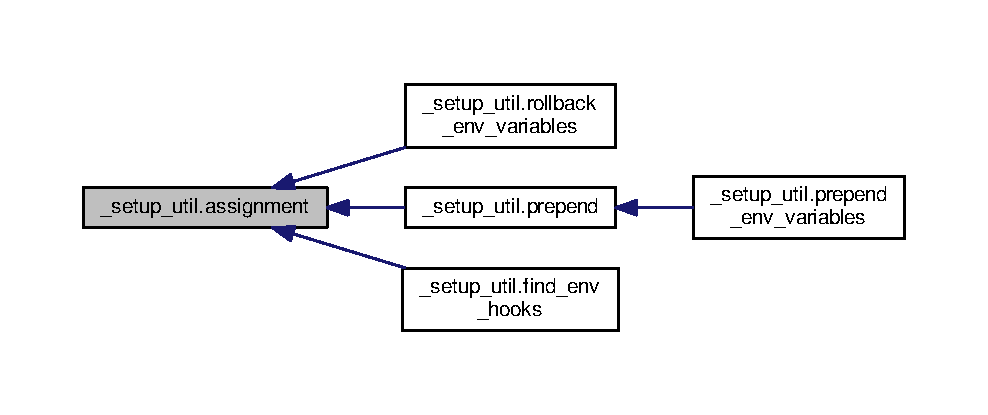
\includegraphics[width=350pt]{namespace__setup__util_ad56c24837fa4eddc63c03fbc7035628f_icgraph}
\end{center}
\end{figure}


\index{\+\_\+setup\+\_\+util@{\+\_\+setup\+\_\+util}!comment@{comment}}
\index{comment@{comment}!\+\_\+setup\+\_\+util@{\+\_\+setup\+\_\+util}}
\subsubsection[{\texorpdfstring{comment(msg)}{comment(msg)}}]{\setlength{\rightskip}{0pt plus 5cm}def \+\_\+setup\+\_\+util.\+comment (
\begin{DoxyParamCaption}
\item[{}]{msg}
\end{DoxyParamCaption}
)}\hypertarget{namespace__setup__util_abe8c95c4cfe8b1374dacd5f91d984353}{}\label{namespace__setup__util_abe8c95c4cfe8b1374dacd5f91d984353}


Definition at line 182 of file \+\_\+setup\+\_\+util.\+py.



Here is the caller graph for this function\+:
\nopagebreak
\begin{figure}[H]
\begin{center}
\leavevmode
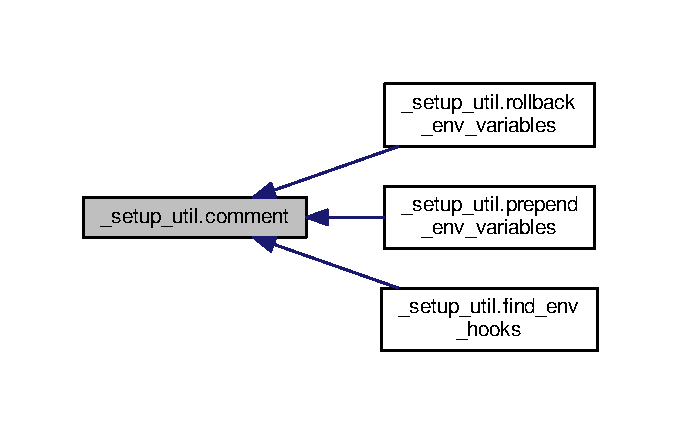
\includegraphics[width=327pt]{namespace__setup__util_abe8c95c4cfe8b1374dacd5f91d984353_icgraph}
\end{center}
\end{figure}


\index{\+\_\+setup\+\_\+util@{\+\_\+setup\+\_\+util}!find\+\_\+env\+\_\+hooks@{find\+\_\+env\+\_\+hooks}}
\index{find\+\_\+env\+\_\+hooks@{find\+\_\+env\+\_\+hooks}!\+\_\+setup\+\_\+util@{\+\_\+setup\+\_\+util}}
\subsubsection[{\texorpdfstring{find\+\_\+env\+\_\+hooks(environ, cmake\+\_\+prefix\+\_\+path)}{find_env_hooks(environ, cmake_prefix_path)}}]{\setlength{\rightskip}{0pt plus 5cm}def \+\_\+setup\+\_\+util.\+find\+\_\+env\+\_\+hooks (
\begin{DoxyParamCaption}
\item[{}]{environ, }
\item[{}]{cmake\+\_\+prefix\+\_\+path}
\end{DoxyParamCaption}
)}\hypertarget{namespace__setup__util_a73de35ca77f260af6691470342ab49ce}{}\label{namespace__setup__util_a73de35ca77f260af6691470342ab49ce}
\begin{DoxyVerb}Generate shell code with found environment hooks
for the all workspaces.
\end{DoxyVerb}
 

Definition at line 198 of file \+\_\+setup\+\_\+util.\+py.



Here is the call graph for this function\+:
\nopagebreak
\begin{figure}[H]
\begin{center}
\leavevmode
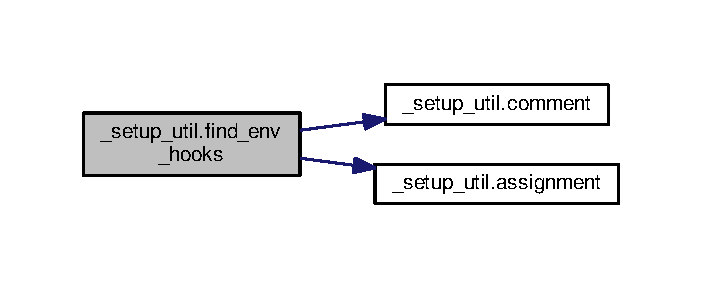
\includegraphics[width=337pt]{namespace__setup__util_a73de35ca77f260af6691470342ab49ce_cgraph}
\end{center}
\end{figure}


\index{\+\_\+setup\+\_\+util@{\+\_\+setup\+\_\+util}!prepend@{prepend}}
\index{prepend@{prepend}!\+\_\+setup\+\_\+util@{\+\_\+setup\+\_\+util}}
\subsubsection[{\texorpdfstring{prepend(environ, key, prefix)}{prepend(environ, key, prefix)}}]{\setlength{\rightskip}{0pt plus 5cm}def \+\_\+setup\+\_\+util.\+prepend (
\begin{DoxyParamCaption}
\item[{}]{environ, }
\item[{}]{key, }
\item[{}]{prefix}
\end{DoxyParamCaption}
)}\hypertarget{namespace__setup__util_ae78d86b2c4279f5b8b1acaa146c35802}{}\label{namespace__setup__util_ae78d86b2c4279f5b8b1acaa146c35802}


Definition at line 189 of file \+\_\+setup\+\_\+util.\+py.



Here is the call graph for this function\+:
\nopagebreak
\begin{figure}[H]
\begin{center}
\leavevmode
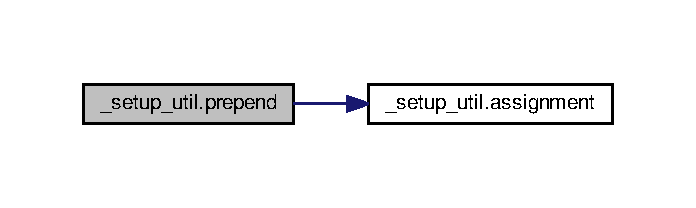
\includegraphics[width=334pt]{namespace__setup__util_ae78d86b2c4279f5b8b1acaa146c35802_cgraph}
\end{center}
\end{figure}




Here is the caller graph for this function\+:
\nopagebreak
\begin{figure}[H]
\begin{center}
\leavevmode
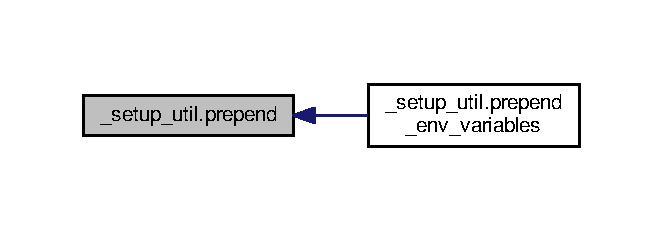
\includegraphics[width=318pt]{namespace__setup__util_ae78d86b2c4279f5b8b1acaa146c35802_icgraph}
\end{center}
\end{figure}


\index{\+\_\+setup\+\_\+util@{\+\_\+setup\+\_\+util}!prepend\+\_\+env\+\_\+variables@{prepend\+\_\+env\+\_\+variables}}
\index{prepend\+\_\+env\+\_\+variables@{prepend\+\_\+env\+\_\+variables}!\+\_\+setup\+\_\+util@{\+\_\+setup\+\_\+util}}
\subsubsection[{\texorpdfstring{prepend\+\_\+env\+\_\+variables(environ, env\+\_\+var\+\_\+subfolders, workspaces)}{prepend_env_variables(environ, env_var_subfolders, workspaces)}}]{\setlength{\rightskip}{0pt plus 5cm}def \+\_\+setup\+\_\+util.\+prepend\+\_\+env\+\_\+variables (
\begin{DoxyParamCaption}
\item[{}]{environ, }
\item[{}]{env\+\_\+var\+\_\+subfolders, }
\item[{}]{workspaces}
\end{DoxyParamCaption}
)}\hypertarget{namespace__setup__util_a832417d18b85bd1d276a87547e86f860}{}\label{namespace__setup__util_a832417d18b85bd1d276a87547e86f860}
\begin{DoxyVerb}Generate shell code to prepend environment variables
for the all workspaces.
\end{DoxyVerb}
 

Definition at line 129 of file \+\_\+setup\+\_\+util.\+py.



Here is the call graph for this function\+:
\nopagebreak
\begin{figure}[H]
\begin{center}
\leavevmode
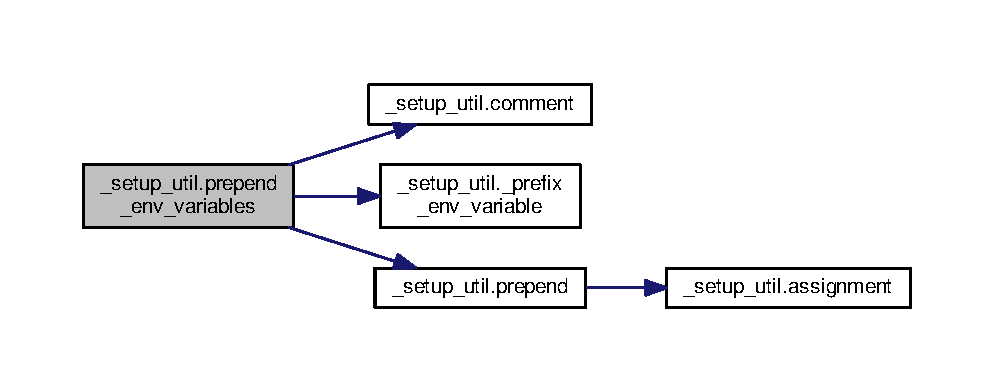
\includegraphics[width=350pt]{namespace__setup__util_a832417d18b85bd1d276a87547e86f860_cgraph}
\end{center}
\end{figure}


\index{\+\_\+setup\+\_\+util@{\+\_\+setup\+\_\+util}!rollback\+\_\+env\+\_\+variables@{rollback\+\_\+env\+\_\+variables}}
\index{rollback\+\_\+env\+\_\+variables@{rollback\+\_\+env\+\_\+variables}!\+\_\+setup\+\_\+util@{\+\_\+setup\+\_\+util}}
\subsubsection[{\texorpdfstring{rollback\+\_\+env\+\_\+variables(environ, env\+\_\+var\+\_\+subfolders)}{rollback_env_variables(environ, env_var_subfolders)}}]{\setlength{\rightskip}{0pt plus 5cm}def \+\_\+setup\+\_\+util.\+rollback\+\_\+env\+\_\+variables (
\begin{DoxyParamCaption}
\item[{}]{environ, }
\item[{}]{env\+\_\+var\+\_\+subfolders}
\end{DoxyParamCaption}
)}\hypertarget{namespace__setup__util_af3030db6102b5aa35cd354a2fb6cca03}{}\label{namespace__setup__util_af3030db6102b5aa35cd354a2fb6cca03}
\begin{DoxyVerb}Generate shell code to reset environment variables
by unrolling modifications based on all workspaces in CMAKE_PREFIX_PATH.
This does not cover modifications performed by environment hooks.
\end{DoxyVerb}
 

Definition at line 62 of file \+\_\+setup\+\_\+util.\+py.



Here is the call graph for this function\+:
\nopagebreak
\begin{figure}[H]
\begin{center}
\leavevmode
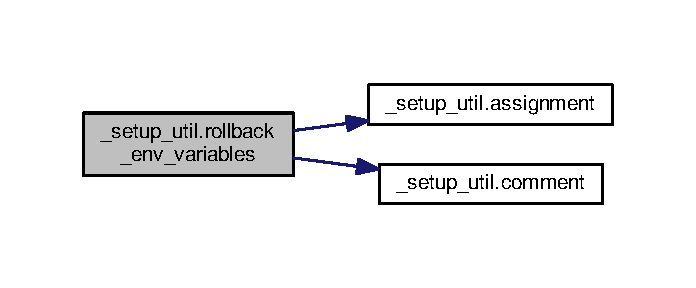
\includegraphics[width=334pt]{namespace__setup__util_af3030db6102b5aa35cd354a2fb6cca03_cgraph}
\end{center}
\end{figure}




\subsection{Variable Documentation}
\index{\+\_\+setup\+\_\+util@{\+\_\+setup\+\_\+util}!args@{args}}
\index{args@{args}!\+\_\+setup\+\_\+util@{\+\_\+setup\+\_\+util}}
\subsubsection[{\texorpdfstring{args}{args}}]{\setlength{\rightskip}{0pt plus 5cm}\+\_\+setup\+\_\+util.\+args = \+\_\+parse\+\_\+arguments()}\hypertarget{namespace__setup__util_a547963d07c6371df1c51b1384a2dec28}{}\label{namespace__setup__util_a547963d07c6371df1c51b1384a2dec28}


Definition at line 259 of file \+\_\+setup\+\_\+util.\+py.

\index{\+\_\+setup\+\_\+util@{\+\_\+setup\+\_\+util}!base\+\_\+path@{base\+\_\+path}}
\index{base\+\_\+path@{base\+\_\+path}!\+\_\+setup\+\_\+util@{\+\_\+setup\+\_\+util}}
\subsubsection[{\texorpdfstring{base\+\_\+path}{base_path}}]{\setlength{\rightskip}{0pt plus 5cm}\+\_\+setup\+\_\+util.\+base\+\_\+path = os.\+path.\+dirname(\+\_\+\+\_\+file\+\_\+\+\_\+)}\hypertarget{namespace__setup__util_a83d25140acd7788bbcb95843fe38e639}{}\label{namespace__setup__util_a83d25140acd7788bbcb95843fe38e639}


Definition at line 267 of file \+\_\+setup\+\_\+util.\+py.

\index{\+\_\+setup\+\_\+util@{\+\_\+setup\+\_\+util}!C\+A\+T\+K\+I\+N\+\_\+\+M\+A\+R\+K\+E\+R\+\_\+\+F\+I\+LE@{C\+A\+T\+K\+I\+N\+\_\+\+M\+A\+R\+K\+E\+R\+\_\+\+F\+I\+LE}}
\index{C\+A\+T\+K\+I\+N\+\_\+\+M\+A\+R\+K\+E\+R\+\_\+\+F\+I\+LE@{C\+A\+T\+K\+I\+N\+\_\+\+M\+A\+R\+K\+E\+R\+\_\+\+F\+I\+LE}!\+\_\+setup\+\_\+util@{\+\_\+setup\+\_\+util}}
\subsubsection[{\texorpdfstring{C\+A\+T\+K\+I\+N\+\_\+\+M\+A\+R\+K\+E\+R\+\_\+\+F\+I\+LE}{CATKIN_MARKER_FILE}}]{\setlength{\rightskip}{0pt plus 5cm}string \+\_\+setup\+\_\+util.\+C\+A\+T\+K\+I\+N\+\_\+\+M\+A\+R\+K\+E\+R\+\_\+\+F\+I\+LE = \textquotesingle{}.catkin\textquotesingle{}}\hypertarget{namespace__setup__util_a3fa0ca5a460a71a43cbc3d4954ab1f10}{}\label{namespace__setup__util_a3fa0ca5a460a71a43cbc3d4954ab1f10}


Definition at line 46 of file \+\_\+setup\+\_\+util.\+py.

\index{\+\_\+setup\+\_\+util@{\+\_\+setup\+\_\+util}!C\+M\+A\+K\+E\+\_\+\+P\+R\+E\+F\+I\+X\+\_\+\+P\+A\+TH@{C\+M\+A\+K\+E\+\_\+\+P\+R\+E\+F\+I\+X\+\_\+\+P\+A\+TH}}
\index{C\+M\+A\+K\+E\+\_\+\+P\+R\+E\+F\+I\+X\+\_\+\+P\+A\+TH@{C\+M\+A\+K\+E\+\_\+\+P\+R\+E\+F\+I\+X\+\_\+\+P\+A\+TH}!\+\_\+setup\+\_\+util@{\+\_\+setup\+\_\+util}}
\subsubsection[{\texorpdfstring{C\+M\+A\+K\+E\+\_\+\+P\+R\+E\+F\+I\+X\+\_\+\+P\+A\+TH}{CMAKE_PREFIX_PATH}}]{\setlength{\rightskip}{0pt plus 5cm}string \+\_\+setup\+\_\+util.\+C\+M\+A\+K\+E\+\_\+\+P\+R\+E\+F\+I\+X\+\_\+\+P\+A\+TH = \textquotesingle{}/home/jbs/catkin\+\_\+ws/devel;/opt/ros/kinetic\textquotesingle{}}\hypertarget{namespace__setup__util_a57afd3d2c076955fb715f3e72ef098eb}{}\label{namespace__setup__util_a57afd3d2c076955fb715f3e72ef098eb}


Definition at line 265 of file \+\_\+setup\+\_\+util.\+py.

\index{\+\_\+setup\+\_\+util@{\+\_\+setup\+\_\+util}!e@{e}}
\index{e@{e}!\+\_\+setup\+\_\+util@{\+\_\+setup\+\_\+util}}
\subsubsection[{\texorpdfstring{e}{e}}]{\setlength{\rightskip}{0pt plus 5cm}\+\_\+setup\+\_\+util.\+e}\hypertarget{namespace__setup__util_acdce690b925de33d6249bbbfa1109d61}{}\label{namespace__setup__util_acdce690b925de33d6249bbbfa1109d61}


Definition at line 261 of file \+\_\+setup\+\_\+util.\+py.

\index{\+\_\+setup\+\_\+util@{\+\_\+setup\+\_\+util}!E\+N\+V\+\_\+\+V\+A\+R\+\_\+\+S\+U\+B\+F\+O\+L\+D\+E\+RS@{E\+N\+V\+\_\+\+V\+A\+R\+\_\+\+S\+U\+B\+F\+O\+L\+D\+E\+RS}}
\index{E\+N\+V\+\_\+\+V\+A\+R\+\_\+\+S\+U\+B\+F\+O\+L\+D\+E\+RS@{E\+N\+V\+\_\+\+V\+A\+R\+\_\+\+S\+U\+B\+F\+O\+L\+D\+E\+RS}!\+\_\+setup\+\_\+util@{\+\_\+setup\+\_\+util}}
\subsubsection[{\texorpdfstring{E\+N\+V\+\_\+\+V\+A\+R\+\_\+\+S\+U\+B\+F\+O\+L\+D\+E\+RS}{ENV_VAR_SUBFOLDERS}}]{\setlength{\rightskip}{0pt plus 5cm}dictionary \+\_\+setup\+\_\+util.\+E\+N\+V\+\_\+\+V\+A\+R\+\_\+\+S\+U\+B\+F\+O\+L\+D\+E\+RS}\hypertarget{namespace__setup__util_aa31804f1be8660156ce9394b33c68dc4}{}\label{namespace__setup__util_aa31804f1be8660156ce9394b33c68dc4}
{\bfseries Initial value\+:}
\begin{DoxyCode}
1 = \{
2     \textcolor{stringliteral}{'CMAKE\_PREFIX\_PATH'}: \textcolor{stringliteral}{''},
3     \textcolor{stringliteral}{'LD\_LIBRARY\_PATH'} \textcolor{keywordflow}{if} \textcolor{keywordflow}{not} IS\_DARWIN \textcolor{keywordflow}{else} \textcolor{stringliteral}{'DYLD\_LIBRARY\_PATH'}: [\textcolor{stringliteral}{'lib'}, os.path.join(\textcolor{stringliteral}{'lib'}, \textcolor{stringliteral}{'
      x86\_64-linux-gnu'})],
4     \textcolor{stringliteral}{'PATH'}: \textcolor{stringliteral}{'bin'},
5     \textcolor{stringliteral}{'PKG\_CONFIG\_PATH'}: [os.path.join(\textcolor{stringliteral}{'lib'}, \textcolor{stringliteral}{'pkgconfig'}), os.path.join(\textcolor{stringliteral}{'lib'}, \textcolor{stringliteral}{'x86\_64-linux-gnu'}, \textcolor{stringliteral}{'
      pkgconfig'})],
6     \textcolor{stringliteral}{'PYTHONPATH'}: \textcolor{stringliteral}{'lib/python2.7/dist-packages'},
7 \}
\end{DoxyCode}


Definition at line 53 of file \+\_\+setup\+\_\+util.\+py.

\index{\+\_\+setup\+\_\+util@{\+\_\+setup\+\_\+util}!environ@{environ}}
\index{environ@{environ}!\+\_\+setup\+\_\+util@{\+\_\+setup\+\_\+util}}
\subsubsection[{\texorpdfstring{environ}{environ}}]{\setlength{\rightskip}{0pt plus 5cm}\+\_\+setup\+\_\+util.\+environ = dict(os.\+environ)}\hypertarget{namespace__setup__util_a9a935bdd9ee1aa0327161025bb18c136}{}\label{namespace__setup__util_a9a935bdd9ee1aa0327161025bb18c136}


Definition at line 272 of file \+\_\+setup\+\_\+util.\+py.

\index{\+\_\+setup\+\_\+util@{\+\_\+setup\+\_\+util}!file@{file}}
\index{file@{file}!\+\_\+setup\+\_\+util@{\+\_\+setup\+\_\+util}}
\subsubsection[{\texorpdfstring{file}{file}}]{\setlength{\rightskip}{0pt plus 5cm}\+\_\+setup\+\_\+util.\+file}\hypertarget{namespace__setup__util_aea63a1b32cc79bc3d872ab7cb30dd07e}{}\label{namespace__setup__util_aea63a1b32cc79bc3d872ab7cb30dd07e}


Definition at line 261 of file \+\_\+setup\+\_\+util.\+py.

\index{\+\_\+setup\+\_\+util@{\+\_\+setup\+\_\+util}!I\+S\+\_\+\+D\+A\+R\+W\+IN@{I\+S\+\_\+\+D\+A\+R\+W\+IN}}
\index{I\+S\+\_\+\+D\+A\+R\+W\+IN@{I\+S\+\_\+\+D\+A\+R\+W\+IN}!\+\_\+setup\+\_\+util@{\+\_\+setup\+\_\+util}}
\subsubsection[{\texorpdfstring{I\+S\+\_\+\+D\+A\+R\+W\+IN}{IS_DARWIN}}]{\setlength{\rightskip}{0pt plus 5cm}tuple \+\_\+setup\+\_\+util.\+I\+S\+\_\+\+D\+A\+R\+W\+IN = ({\bf system} == \textquotesingle{}Darwin\textquotesingle{})}\hypertarget{namespace__setup__util_aecbb100ce6f94bb3c7e16d58fde05f96}{}\label{namespace__setup__util_aecbb100ce6f94bb3c7e16d58fde05f96}


Definition at line 49 of file \+\_\+setup\+\_\+util.\+py.

\index{\+\_\+setup\+\_\+util@{\+\_\+setup\+\_\+util}!I\+S\+\_\+\+W\+I\+N\+D\+O\+WS@{I\+S\+\_\+\+W\+I\+N\+D\+O\+WS}}
\index{I\+S\+\_\+\+W\+I\+N\+D\+O\+WS@{I\+S\+\_\+\+W\+I\+N\+D\+O\+WS}!\+\_\+setup\+\_\+util@{\+\_\+setup\+\_\+util}}
\subsubsection[{\texorpdfstring{I\+S\+\_\+\+W\+I\+N\+D\+O\+WS}{IS_WINDOWS}}]{\setlength{\rightskip}{0pt plus 5cm}tuple \+\_\+setup\+\_\+util.\+I\+S\+\_\+\+W\+I\+N\+D\+O\+WS = ({\bf system} == \textquotesingle{}Windows\textquotesingle{})}\hypertarget{namespace__setup__util_a6fe69c2dbd92959b6651a28cbb846e6e}{}\label{namespace__setup__util_a6fe69c2dbd92959b6651a28cbb846e6e}


Definition at line 50 of file \+\_\+setup\+\_\+util.\+py.

\index{\+\_\+setup\+\_\+util@{\+\_\+setup\+\_\+util}!lines@{lines}}
\index{lines@{lines}!\+\_\+setup\+\_\+util@{\+\_\+setup\+\_\+util}}
\subsubsection[{\texorpdfstring{lines}{lines}}]{\setlength{\rightskip}{0pt plus 5cm}list \+\_\+setup\+\_\+util.\+lines = \mbox{[}$\,$\mbox{]}}\hypertarget{namespace__setup__util_a8618d8be5f729d4c9696daa5e083a001}{}\label{namespace__setup__util_a8618d8be5f729d4c9696daa5e083a001}


Definition at line 273 of file \+\_\+setup\+\_\+util.\+py.

\index{\+\_\+setup\+\_\+util@{\+\_\+setup\+\_\+util}!system@{system}}
\index{system@{system}!\+\_\+setup\+\_\+util@{\+\_\+setup\+\_\+util}}
\subsubsection[{\texorpdfstring{system}{system}}]{\setlength{\rightskip}{0pt plus 5cm}\+\_\+setup\+\_\+util.\+system = platform.\+system()}\hypertarget{namespace__setup__util_ae9fca6a80a6923f4580be72f68fee325}{}\label{namespace__setup__util_ae9fca6a80a6923f4580be72f68fee325}


Definition at line 48 of file \+\_\+setup\+\_\+util.\+py.


\hypertarget{namespacechaser}{}\section{chaser Namespace Reference}
\label{namespacechaser}\index{chaser@{chaser}}
\subsection*{Classes}
\begin{DoxyCompactItemize}
\item 
struct \hyperlink{structchaser_1_1_preplanner_params}{Preplanner\+Params}
\item 
struct \hyperlink{structchaser_1_1_smoothplanner_params}{Smoothplanner\+Params}
\end{DoxyCompactItemize}

\hypertarget{namespacegenerate__cached__setup}{}\section{generate\+\_\+cached\+\_\+setup Namespace Reference}
\label{namespacegenerate__cached__setup}\index{generate\+\_\+cached\+\_\+setup@{generate\+\_\+cached\+\_\+setup}}
\subsection*{Variables}
\begin{DoxyCompactItemize}
\item 
\hyperlink{namespacegenerate__cached__setup_a72579fd01529a79bab20d99291889d3f}{python\+\_\+path} = os.\+path.\+join(workspace, \textquotesingle{}lib/python2.\+7/dist-\/packages\textquotesingle{})
\item 
\hyperlink{namespacegenerate__cached__setup_a52601295006f2366a311c4453d8f2f2e}{code} = generate\+\_\+environment\+\_\+script(\textquotesingle{}/home/jbs/catkin\+\_\+ws/src/auto\+\_\+chaser/build/devel/env.\+sh\textquotesingle{})
\item 
string \hyperlink{namespacegenerate__cached__setup_a0265aee5075ee1eb701ff69c98ad6793}{output\+\_\+filename} = \textquotesingle{}/home/jbs/catkin\+\_\+ws/src/auto\+\_\+chaser/build/catkin\+\_\+generated/setup\+\_\+cached.\+sh\textquotesingle{}
\item 
\hyperlink{namespacegenerate__cached__setup_a10081e5abedae9bd46dd91202096e789}{mode} = os.\+stat(\hyperlink{namespacegenerate__cached__setup_a0265aee5075ee1eb701ff69c98ad6793}{output\+\_\+filename}).st\+\_\+mode
\end{DoxyCompactItemize}


\subsection{Variable Documentation}
\index{generate\+\_\+cached\+\_\+setup@{generate\+\_\+cached\+\_\+setup}!code@{code}}
\index{code@{code}!generate\+\_\+cached\+\_\+setup@{generate\+\_\+cached\+\_\+setup}}
\subsubsection[{\texorpdfstring{code}{code}}]{\setlength{\rightskip}{0pt plus 5cm}generate\+\_\+cached\+\_\+setup.\+code = generate\+\_\+environment\+\_\+script(\textquotesingle{}/home/jbs/catkin\+\_\+ws/src/auto\+\_\+chaser/build/devel/env.\+sh\textquotesingle{})}\hypertarget{namespacegenerate__cached__setup_a52601295006f2366a311c4453d8f2f2e}{}\label{namespacegenerate__cached__setup_a52601295006f2366a311c4453d8f2f2e}
\index{generate\+\_\+cached\+\_\+setup@{generate\+\_\+cached\+\_\+setup}!mode@{mode}}
\index{mode@{mode}!generate\+\_\+cached\+\_\+setup@{generate\+\_\+cached\+\_\+setup}}
\subsubsection[{\texorpdfstring{mode}{mode}}]{\setlength{\rightskip}{0pt plus 5cm}generate\+\_\+cached\+\_\+setup.\+mode = os.\+stat({\bf output\+\_\+filename}).st\+\_\+mode}\hypertarget{namespacegenerate__cached__setup_a10081e5abedae9bd46dd91202096e789}{}\label{namespacegenerate__cached__setup_a10081e5abedae9bd46dd91202096e789}
\index{generate\+\_\+cached\+\_\+setup@{generate\+\_\+cached\+\_\+setup}!output\+\_\+filename@{output\+\_\+filename}}
\index{output\+\_\+filename@{output\+\_\+filename}!generate\+\_\+cached\+\_\+setup@{generate\+\_\+cached\+\_\+setup}}
\subsubsection[{\texorpdfstring{output\+\_\+filename}{output_filename}}]{\setlength{\rightskip}{0pt plus 5cm}string generate\+\_\+cached\+\_\+setup.\+output\+\_\+filename = \textquotesingle{}/home/jbs/catkin\+\_\+ws/src/auto\+\_\+chaser/build/catkin\+\_\+generated/setup\+\_\+cached.\+sh\textquotesingle{}}\hypertarget{namespacegenerate__cached__setup_a0265aee5075ee1eb701ff69c98ad6793}{}\label{namespacegenerate__cached__setup_a0265aee5075ee1eb701ff69c98ad6793}
\index{generate\+\_\+cached\+\_\+setup@{generate\+\_\+cached\+\_\+setup}!python\+\_\+path@{python\+\_\+path}}
\index{python\+\_\+path@{python\+\_\+path}!generate\+\_\+cached\+\_\+setup@{generate\+\_\+cached\+\_\+setup}}
\subsubsection[{\texorpdfstring{python\+\_\+path}{python_path}}]{\setlength{\rightskip}{0pt plus 5cm}generate\+\_\+cached\+\_\+setup.\+python\+\_\+path = os.\+path.\+join(workspace, \textquotesingle{}lib/python2.\+7/dist-\/packages\textquotesingle{})}\hypertarget{namespacegenerate__cached__setup_a72579fd01529a79bab20d99291889d3f}{}\label{namespacegenerate__cached__setup_a72579fd01529a79bab20d99291889d3f}

\hypertarget{namespacepkg}{}\section{pkg Namespace Reference}
\label{namespacepkg}\index{pkg@{pkg}}
\subsection*{Variables}
\begin{DoxyCompactItemize}
\item 
string \hyperlink{namespacepkg_ae26c7a5a06b7d738f4d210ca449e6bee}{C\+A\+T\+K\+I\+N\+\_\+\+P\+A\+C\+K\+A\+G\+E\+\_\+\+P\+R\+E\+F\+IX} = \char`\"{}\char`\"{}
\item 
string \hyperlink{namespacepkg_a2760bf8266ff58da440f65ee91b203ab}{P\+R\+O\+J\+E\+C\+T\+\_\+\+P\+K\+G\+\_\+\+C\+O\+N\+F\+I\+G\+\_\+\+I\+N\+C\+L\+U\+D\+E\+\_\+\+D\+I\+RS} = \char`\"{}/home/jbs/catkin\+\_\+ws/src/auto\+\_\+chaser/include\char`\"{}
\item 
string \hyperlink{namespacepkg_a17c18447fad253ee1c0d76deec88028c}{P\+R\+O\+J\+E\+C\+T\+\_\+\+C\+A\+T\+K\+I\+N\+\_\+\+D\+E\+P\+E\+N\+DS} = \char`\"{}\char`\"{}
\item 
string \hyperlink{namespacepkg_a433e30cecb4a0123a7c4b384d168e336}{P\+K\+G\+\_\+\+C\+O\+N\+F\+I\+G\+\_\+\+L\+I\+B\+R\+A\+R\+I\+E\+S\+\_\+\+W\+I\+T\+H\+\_\+\+P\+R\+E\+F\+IX} = \char`\"{}-\/ltraj\+\_\+gen\+\_\+chasing\char`\"{}
\item 
string \hyperlink{namespacepkg_a7dfbe99257c26f5e4a3a5483995d9ddc}{P\+R\+O\+J\+E\+C\+T\+\_\+\+N\+A\+ME} = \char`\"{}auto\+\_\+chaser\char`\"{}
\item 
string \hyperlink{namespacepkg_a3f0f1b4bc03c596525e025539ca4332f}{P\+R\+O\+J\+E\+C\+T\+\_\+\+S\+P\+A\+C\+E\+\_\+\+D\+IR} = \char`\"{}/home/jbs/catkin\+\_\+ws/src/auto\+\_\+chaser/build/devel\char`\"{}
\item 
string \hyperlink{namespacepkg_ab1037914b9286bb61855131c06149648}{P\+R\+O\+J\+E\+C\+T\+\_\+\+V\+E\+R\+S\+I\+ON} = \char`\"{}0.\+0.\+0\char`\"{}
\end{DoxyCompactItemize}


\subsection{Variable Documentation}
\index{pkg@{pkg}!C\+A\+T\+K\+I\+N\+\_\+\+P\+A\+C\+K\+A\+G\+E\+\_\+\+P\+R\+E\+F\+IX@{C\+A\+T\+K\+I\+N\+\_\+\+P\+A\+C\+K\+A\+G\+E\+\_\+\+P\+R\+E\+F\+IX}}
\index{C\+A\+T\+K\+I\+N\+\_\+\+P\+A\+C\+K\+A\+G\+E\+\_\+\+P\+R\+E\+F\+IX@{C\+A\+T\+K\+I\+N\+\_\+\+P\+A\+C\+K\+A\+G\+E\+\_\+\+P\+R\+E\+F\+IX}!pkg@{pkg}}
\subsubsection[{\texorpdfstring{C\+A\+T\+K\+I\+N\+\_\+\+P\+A\+C\+K\+A\+G\+E\+\_\+\+P\+R\+E\+F\+IX}{CATKIN_PACKAGE_PREFIX}}]{\setlength{\rightskip}{0pt plus 5cm}string pkg.\+C\+A\+T\+K\+I\+N\+\_\+\+P\+A\+C\+K\+A\+G\+E\+\_\+\+P\+R\+E\+F\+IX = \char`\"{}\char`\"{}}\hypertarget{namespacepkg_ae26c7a5a06b7d738f4d210ca449e6bee}{}\label{namespacepkg_ae26c7a5a06b7d738f4d210ca449e6bee}


Definition at line 2 of file pkg.\+develspace.\+context.\+pc.\+py.

\index{pkg@{pkg}!P\+K\+G\+\_\+\+C\+O\+N\+F\+I\+G\+\_\+\+L\+I\+B\+R\+A\+R\+I\+E\+S\+\_\+\+W\+I\+T\+H\+\_\+\+P\+R\+E\+F\+IX@{P\+K\+G\+\_\+\+C\+O\+N\+F\+I\+G\+\_\+\+L\+I\+B\+R\+A\+R\+I\+E\+S\+\_\+\+W\+I\+T\+H\+\_\+\+P\+R\+E\+F\+IX}}
\index{P\+K\+G\+\_\+\+C\+O\+N\+F\+I\+G\+\_\+\+L\+I\+B\+R\+A\+R\+I\+E\+S\+\_\+\+W\+I\+T\+H\+\_\+\+P\+R\+E\+F\+IX@{P\+K\+G\+\_\+\+C\+O\+N\+F\+I\+G\+\_\+\+L\+I\+B\+R\+A\+R\+I\+E\+S\+\_\+\+W\+I\+T\+H\+\_\+\+P\+R\+E\+F\+IX}!pkg@{pkg}}
\subsubsection[{\texorpdfstring{P\+K\+G\+\_\+\+C\+O\+N\+F\+I\+G\+\_\+\+L\+I\+B\+R\+A\+R\+I\+E\+S\+\_\+\+W\+I\+T\+H\+\_\+\+P\+R\+E\+F\+IX}{PKG_CONFIG_LIBRARIES_WITH_PREFIX}}]{\setlength{\rightskip}{0pt plus 5cm}string pkg.\+P\+K\+G\+\_\+\+C\+O\+N\+F\+I\+G\+\_\+\+L\+I\+B\+R\+A\+R\+I\+E\+S\+\_\+\+W\+I\+T\+H\+\_\+\+P\+R\+E\+F\+IX = \char`\"{}-\/ltraj\+\_\+gen\+\_\+chasing\char`\"{}}\hypertarget{namespacepkg_a433e30cecb4a0123a7c4b384d168e336}{}\label{namespacepkg_a433e30cecb4a0123a7c4b384d168e336}


Definition at line 5 of file pkg.\+develspace.\+context.\+pc.\+py.

\index{pkg@{pkg}!P\+R\+O\+J\+E\+C\+T\+\_\+\+C\+A\+T\+K\+I\+N\+\_\+\+D\+E\+P\+E\+N\+DS@{P\+R\+O\+J\+E\+C\+T\+\_\+\+C\+A\+T\+K\+I\+N\+\_\+\+D\+E\+P\+E\+N\+DS}}
\index{P\+R\+O\+J\+E\+C\+T\+\_\+\+C\+A\+T\+K\+I\+N\+\_\+\+D\+E\+P\+E\+N\+DS@{P\+R\+O\+J\+E\+C\+T\+\_\+\+C\+A\+T\+K\+I\+N\+\_\+\+D\+E\+P\+E\+N\+DS}!pkg@{pkg}}
\subsubsection[{\texorpdfstring{P\+R\+O\+J\+E\+C\+T\+\_\+\+C\+A\+T\+K\+I\+N\+\_\+\+D\+E\+P\+E\+N\+DS}{PROJECT_CATKIN_DEPENDS}}]{\setlength{\rightskip}{0pt plus 5cm}string pkg.\+P\+R\+O\+J\+E\+C\+T\+\_\+\+C\+A\+T\+K\+I\+N\+\_\+\+D\+E\+P\+E\+N\+DS = \char`\"{}\char`\"{}}\hypertarget{namespacepkg_a17c18447fad253ee1c0d76deec88028c}{}\label{namespacepkg_a17c18447fad253ee1c0d76deec88028c}


Definition at line 4 of file pkg.\+develspace.\+context.\+pc.\+py.

\index{pkg@{pkg}!P\+R\+O\+J\+E\+C\+T\+\_\+\+N\+A\+ME@{P\+R\+O\+J\+E\+C\+T\+\_\+\+N\+A\+ME}}
\index{P\+R\+O\+J\+E\+C\+T\+\_\+\+N\+A\+ME@{P\+R\+O\+J\+E\+C\+T\+\_\+\+N\+A\+ME}!pkg@{pkg}}
\subsubsection[{\texorpdfstring{P\+R\+O\+J\+E\+C\+T\+\_\+\+N\+A\+ME}{PROJECT_NAME}}]{\setlength{\rightskip}{0pt plus 5cm}string pkg.\+P\+R\+O\+J\+E\+C\+T\+\_\+\+N\+A\+ME = \char`\"{}auto\+\_\+chaser\char`\"{}}\hypertarget{namespacepkg_a7dfbe99257c26f5e4a3a5483995d9ddc}{}\label{namespacepkg_a7dfbe99257c26f5e4a3a5483995d9ddc}


Definition at line 6 of file pkg.\+develspace.\+context.\+pc.\+py.

\index{pkg@{pkg}!P\+R\+O\+J\+E\+C\+T\+\_\+\+P\+K\+G\+\_\+\+C\+O\+N\+F\+I\+G\+\_\+\+I\+N\+C\+L\+U\+D\+E\+\_\+\+D\+I\+RS@{P\+R\+O\+J\+E\+C\+T\+\_\+\+P\+K\+G\+\_\+\+C\+O\+N\+F\+I\+G\+\_\+\+I\+N\+C\+L\+U\+D\+E\+\_\+\+D\+I\+RS}}
\index{P\+R\+O\+J\+E\+C\+T\+\_\+\+P\+K\+G\+\_\+\+C\+O\+N\+F\+I\+G\+\_\+\+I\+N\+C\+L\+U\+D\+E\+\_\+\+D\+I\+RS@{P\+R\+O\+J\+E\+C\+T\+\_\+\+P\+K\+G\+\_\+\+C\+O\+N\+F\+I\+G\+\_\+\+I\+N\+C\+L\+U\+D\+E\+\_\+\+D\+I\+RS}!pkg@{pkg}}
\subsubsection[{\texorpdfstring{P\+R\+O\+J\+E\+C\+T\+\_\+\+P\+K\+G\+\_\+\+C\+O\+N\+F\+I\+G\+\_\+\+I\+N\+C\+L\+U\+D\+E\+\_\+\+D\+I\+RS}{PROJECT_PKG_CONFIG_INCLUDE_DIRS}}]{\setlength{\rightskip}{0pt plus 5cm}string pkg.\+P\+R\+O\+J\+E\+C\+T\+\_\+\+P\+K\+G\+\_\+\+C\+O\+N\+F\+I\+G\+\_\+\+I\+N\+C\+L\+U\+D\+E\+\_\+\+D\+I\+RS = \char`\"{}/home/jbs/catkin\+\_\+ws/src/auto\+\_\+chaser/include\char`\"{}}\hypertarget{namespacepkg_a2760bf8266ff58da440f65ee91b203ab}{}\label{namespacepkg_a2760bf8266ff58da440f65ee91b203ab}


Definition at line 3 of file pkg.\+develspace.\+context.\+pc.\+py.

\index{pkg@{pkg}!P\+R\+O\+J\+E\+C\+T\+\_\+\+S\+P\+A\+C\+E\+\_\+\+D\+IR@{P\+R\+O\+J\+E\+C\+T\+\_\+\+S\+P\+A\+C\+E\+\_\+\+D\+IR}}
\index{P\+R\+O\+J\+E\+C\+T\+\_\+\+S\+P\+A\+C\+E\+\_\+\+D\+IR@{P\+R\+O\+J\+E\+C\+T\+\_\+\+S\+P\+A\+C\+E\+\_\+\+D\+IR}!pkg@{pkg}}
\subsubsection[{\texorpdfstring{P\+R\+O\+J\+E\+C\+T\+\_\+\+S\+P\+A\+C\+E\+\_\+\+D\+IR}{PROJECT_SPACE_DIR}}]{\setlength{\rightskip}{0pt plus 5cm}string pkg.\+P\+R\+O\+J\+E\+C\+T\+\_\+\+S\+P\+A\+C\+E\+\_\+\+D\+IR = \char`\"{}/home/jbs/catkin\+\_\+ws/src/auto\+\_\+chaser/build/devel\char`\"{}}\hypertarget{namespacepkg_a3f0f1b4bc03c596525e025539ca4332f}{}\label{namespacepkg_a3f0f1b4bc03c596525e025539ca4332f}


Definition at line 7 of file pkg.\+develspace.\+context.\+pc.\+py.

\index{pkg@{pkg}!P\+R\+O\+J\+E\+C\+T\+\_\+\+V\+E\+R\+S\+I\+ON@{P\+R\+O\+J\+E\+C\+T\+\_\+\+V\+E\+R\+S\+I\+ON}}
\index{P\+R\+O\+J\+E\+C\+T\+\_\+\+V\+E\+R\+S\+I\+ON@{P\+R\+O\+J\+E\+C\+T\+\_\+\+V\+E\+R\+S\+I\+ON}!pkg@{pkg}}
\subsubsection[{\texorpdfstring{P\+R\+O\+J\+E\+C\+T\+\_\+\+V\+E\+R\+S\+I\+ON}{PROJECT_VERSION}}]{\setlength{\rightskip}{0pt plus 5cm}string pkg.\+P\+R\+O\+J\+E\+C\+T\+\_\+\+V\+E\+R\+S\+I\+ON = \char`\"{}0.\+0.\+0\char`\"{}}\hypertarget{namespacepkg_ab1037914b9286bb61855131c06149648}{}\label{namespacepkg_ab1037914b9286bb61855131c06149648}


Definition at line 8 of file pkg.\+develspace.\+context.\+pc.\+py.


\hypertarget{namespace_ui}{}\section{Ui Namespace Reference}
\label{namespace_ui}\index{Ui@{Ui}}
\subsection*{Classes}
\begin{DoxyCompactItemize}
\item 
class \hyperlink{class_ui_1_1_main_window}{Main\+Window}
\end{DoxyCompactItemize}

\chapter{Class Documentation}
\hypertarget{class_chaser}{}\section{Chaser Class Reference}
\label{class_chaser}\index{Chaser@{Chaser}}


{\ttfamily \#include $<$Chaser.\+h$>$}

\subsection*{Public Member Functions}
\begin{DoxyCompactItemize}
\item 
\hyperlink{class_chaser_ae1179fa7b77db9c80468f88222e32f09}{Chaser} ()
\item 
void \hyperlink{class_chaser_a3538485980643e885755608e4297d1f6}{init} (ros\+::\+Node\+Handle nh)
\item 
bool \hyperlink{class_chaser_a8feeca68466b9b4576ee9c99b624dfc5}{chase\+\_\+update} (\hyperlink{struct_grid_field}{Grid\+Field} $\ast$global\+\_\+edf, vector$<$ Point $>$ target\+\_\+pnts, Point chaser\+\_\+x0, Twist chaser\+\_\+v0, Twist chaser\+\_\+a0, Time\+Series knots)
\item 
void \hyperlink{class_chaser_a7d736728bb5327acf0d334d7d4b1b844}{session} (double t)
\item 
Point \hyperlink{class_chaser_a6dca60b8af1c63eff3235515255cf355}{eval\+\_\+point} (double t\+\_\+eval)
\item 
Twist \hyperlink{class_chaser_a208374e7b85f9a35c1c00ec4f1ec65c3}{eval\+\_\+velocity} (double t\+\_\+eval)
\item 
Twist \hyperlink{class_chaser_a2fe36102d5a9befcb4c6ada3375260ed}{eval\+\_\+acceleration} (double t\+\_\+eval)
\item 
Point \hyperlink{class_chaser_a7a42e3dd3ca45e343652318e591f87d1}{get\+\_\+control\+\_\+point} (double t\+\_\+eval)
\begin{DoxyCompactList}\small\item\em obtains the latest control point. yaw will be selected from wrapper with information of target \end{DoxyCompactList}\item 
double \hyperlink{class_chaser_aaa7ce7ea18761dd1513cf9e85c6b4e48}{get\+\_\+hovering\+\_\+z} ()
\end{DoxyCompactItemize}
\subsection*{Public Attributes}
\begin{DoxyCompactItemize}
\item 
bool \hyperlink{class_chaser_a53af032471ad6bdc828c4eae78085813}{is\+\_\+complete\+\_\+chasing\+\_\+path}
\item 
bool \hyperlink{class_chaser_a33b880dd48d1d983001fa93ba1a1184f}{is\+\_\+log}
\item 
string \hyperlink{class_chaser_a9d9ad4c7ca00bcda38d2bc809f3e7654}{log\+\_\+dir}
\end{DoxyCompactItemize}


\subsection{Detailed Description}


Definition at line 5 of file Chaser.\+h.



\subsection{Constructor \& Destructor Documentation}
\index{Chaser@{Chaser}!Chaser@{Chaser}}
\index{Chaser@{Chaser}!Chaser@{Chaser}}
\subsubsection[{\texorpdfstring{Chaser()}{Chaser()}}]{\setlength{\rightskip}{0pt plus 5cm}Chaser\+::\+Chaser (
\begin{DoxyParamCaption}
{}
\end{DoxyParamCaption}
)}\hypertarget{class_chaser_ae1179fa7b77db9c80468f88222e32f09}{}\label{class_chaser_ae1179fa7b77db9c80468f88222e32f09}


Definition at line 3 of file Chaser.\+cpp.



\subsection{Member Function Documentation}
\index{Chaser@{Chaser}!chase\+\_\+update@{chase\+\_\+update}}
\index{chase\+\_\+update@{chase\+\_\+update}!Chaser@{Chaser}}
\subsubsection[{\texorpdfstring{chase\+\_\+update(\+Grid\+Field $\ast$global\+\_\+edf, vector$<$ Point $>$ target\+\_\+pnts, Point chaser\+\_\+x0, Twist chaser\+\_\+v0, Twist chaser\+\_\+a0, Time\+Series knots)}{chase_update(GridField *global_edf, vector< Point > target_pnts, Point chaser_x0, Twist chaser_v0, Twist chaser_a0, TimeSeries knots)}}]{\setlength{\rightskip}{0pt plus 5cm}bool Chaser\+::chase\+\_\+update (
\begin{DoxyParamCaption}
\item[{{\bf Grid\+Field} $\ast$}]{global\+\_\+edf, }
\item[{vector$<$ Point $>$}]{target\+\_\+pnts, }
\item[{Point}]{chaser\+\_\+x0, }
\item[{Twist}]{chaser\+\_\+v0, }
\item[{Twist}]{chaser\+\_\+a0, }
\item[{Time\+Series}]{knots}
\end{DoxyParamCaption}
)}\hypertarget{class_chaser_a8feeca68466b9b4576ee9c99b624dfc5}{}\label{class_chaser_a8feeca68466b9b4576ee9c99b624dfc5}


Definition at line 26 of file Chaser.\+cpp.



Here is the call graph for this function\+:
\nopagebreak
\begin{figure}[H]
\begin{center}
\leavevmode
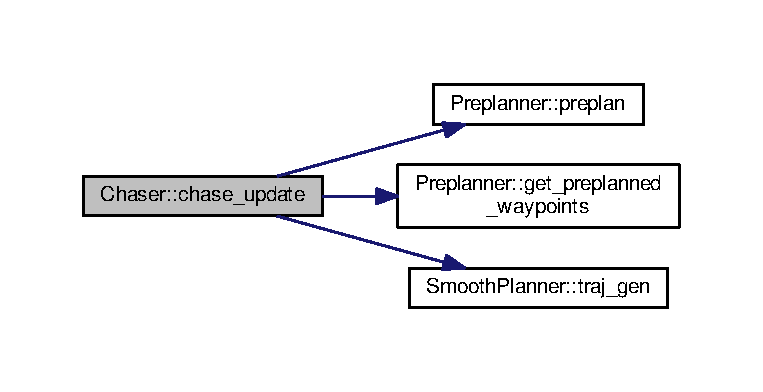
\includegraphics[width=350pt]{class_chaser_a8feeca68466b9b4576ee9c99b624dfc5_cgraph}
\end{center}
\end{figure}


\index{Chaser@{Chaser}!eval\+\_\+acceleration@{eval\+\_\+acceleration}}
\index{eval\+\_\+acceleration@{eval\+\_\+acceleration}!Chaser@{Chaser}}
\subsubsection[{\texorpdfstring{eval\+\_\+acceleration(double t\+\_\+eval)}{eval_acceleration(double t_eval)}}]{\setlength{\rightskip}{0pt plus 5cm}Twist Chaser\+::eval\+\_\+acceleration (
\begin{DoxyParamCaption}
\item[{double}]{t\+\_\+eval}
\end{DoxyParamCaption}
)}\hypertarget{class_chaser_a2fe36102d5a9befcb4c6ada3375260ed}{}\label{class_chaser_a2fe36102d5a9befcb4c6ada3375260ed}


Definition at line 86 of file Chaser.\+cpp.

\index{Chaser@{Chaser}!eval\+\_\+point@{eval\+\_\+point}}
\index{eval\+\_\+point@{eval\+\_\+point}!Chaser@{Chaser}}
\subsubsection[{\texorpdfstring{eval\+\_\+point(double t\+\_\+eval)}{eval_point(double t_eval)}}]{\setlength{\rightskip}{0pt plus 5cm}Point Chaser\+::eval\+\_\+point (
\begin{DoxyParamCaption}
\item[{double}]{t\+\_\+eval}
\end{DoxyParamCaption}
)}\hypertarget{class_chaser_a6dca60b8af1c63eff3235515255cf355}{}\label{class_chaser_a6dca60b8af1c63eff3235515255cf355}


Definition at line 77 of file Chaser.\+cpp.

\index{Chaser@{Chaser}!eval\+\_\+velocity@{eval\+\_\+velocity}}
\index{eval\+\_\+velocity@{eval\+\_\+velocity}!Chaser@{Chaser}}
\subsubsection[{\texorpdfstring{eval\+\_\+velocity(double t\+\_\+eval)}{eval_velocity(double t_eval)}}]{\setlength{\rightskip}{0pt plus 5cm}Twist Chaser\+::eval\+\_\+velocity (
\begin{DoxyParamCaption}
\item[{double}]{t\+\_\+eval}
\end{DoxyParamCaption}
)}\hypertarget{class_chaser_a208374e7b85f9a35c1c00ec4f1ec65c3}{}\label{class_chaser_a208374e7b85f9a35c1c00ec4f1ec65c3}


Definition at line 82 of file Chaser.\+cpp.

\index{Chaser@{Chaser}!get\+\_\+control\+\_\+point@{get\+\_\+control\+\_\+point}}
\index{get\+\_\+control\+\_\+point@{get\+\_\+control\+\_\+point}!Chaser@{Chaser}}
\subsubsection[{\texorpdfstring{get\+\_\+control\+\_\+point(double t\+\_\+eval)}{get_control_point(double t_eval)}}]{\setlength{\rightskip}{0pt plus 5cm}Point Chaser\+::get\+\_\+control\+\_\+point (
\begin{DoxyParamCaption}
\item[{double}]{t\+\_\+eval}
\end{DoxyParamCaption}
)}\hypertarget{class_chaser_a7a42e3dd3ca45e343652318e591f87d1}{}\label{class_chaser_a7a42e3dd3ca45e343652318e591f87d1}


obtains the latest control point. yaw will be selected from wrapper with information of target 


\begin{DoxyParams}{Parameters}
{\em t\+\_\+eval} & evaluation time \\
\hline
\end{DoxyParams}
\begin{DoxyReturn}{Returns}
Point the control point 
\end{DoxyReturn}


Definition at line 97 of file Chaser.\+cpp.

\index{Chaser@{Chaser}!get\+\_\+hovering\+\_\+z@{get\+\_\+hovering\+\_\+z}}
\index{get\+\_\+hovering\+\_\+z@{get\+\_\+hovering\+\_\+z}!Chaser@{Chaser}}
\subsubsection[{\texorpdfstring{get\+\_\+hovering\+\_\+z()}{get_hovering_z()}}]{\setlength{\rightskip}{0pt plus 5cm}double Chaser\+::get\+\_\+hovering\+\_\+z (
\begin{DoxyParamCaption}
{}
\end{DoxyParamCaption}
)}\hypertarget{class_chaser_aaa7ce7ea18761dd1513cf9e85c6b4e48}{}\label{class_chaser_aaa7ce7ea18761dd1513cf9e85c6b4e48}


Definition at line 22 of file Chaser.\+cpp.

\index{Chaser@{Chaser}!init@{init}}
\index{init@{init}!Chaser@{Chaser}}
\subsubsection[{\texorpdfstring{init(ros\+::\+Node\+Handle nh)}{init(ros::NodeHandle nh)}}]{\setlength{\rightskip}{0pt plus 5cm}void Chaser\+::init (
\begin{DoxyParamCaption}
\item[{ros\+::\+Node\+Handle}]{nh}
\end{DoxyParamCaption}
)}\hypertarget{class_chaser_a3538485980643e885755608e4297d1f6}{}\label{class_chaser_a3538485980643e885755608e4297d1f6}


Definition at line 5 of file Chaser.\+cpp.



Here is the call graph for this function\+:
\nopagebreak
\begin{figure}[H]
\begin{center}
\leavevmode
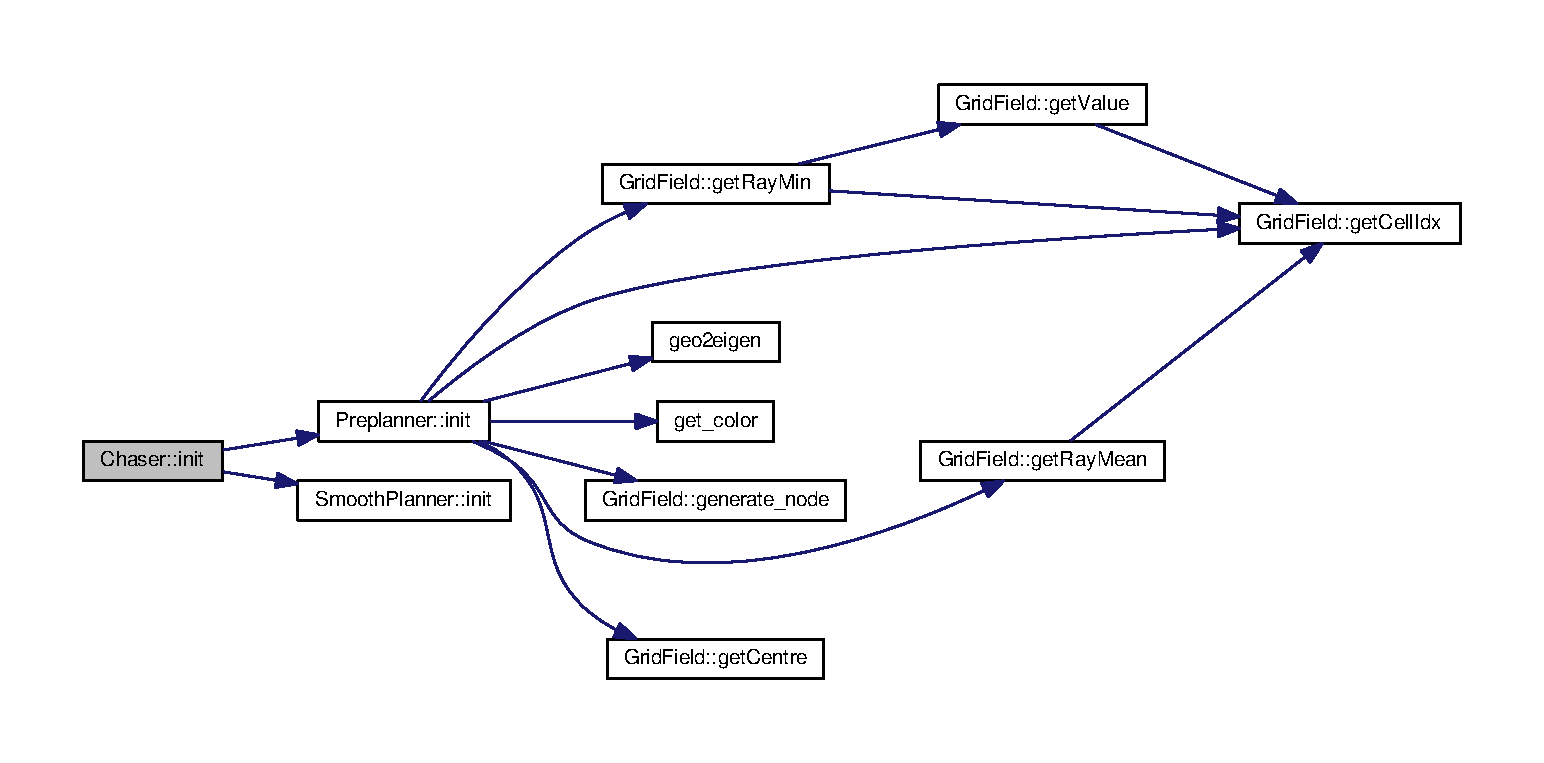
\includegraphics[width=350pt]{class_chaser_a3538485980643e885755608e4297d1f6_cgraph}
\end{center}
\end{figure}


\index{Chaser@{Chaser}!session@{session}}
\index{session@{session}!Chaser@{Chaser}}
\subsubsection[{\texorpdfstring{session(double t)}{session(double t)}}]{\setlength{\rightskip}{0pt plus 5cm}void Chaser\+::session (
\begin{DoxyParamCaption}
\item[{double}]{t}
\end{DoxyParamCaption}
)}\hypertarget{class_chaser_a7d736728bb5327acf0d334d7d4b1b844}{}\label{class_chaser_a7d736728bb5327acf0d334d7d4b1b844}


Definition at line 71 of file Chaser.\+cpp.



Here is the call graph for this function\+:
\nopagebreak
\begin{figure}[H]
\begin{center}
\leavevmode
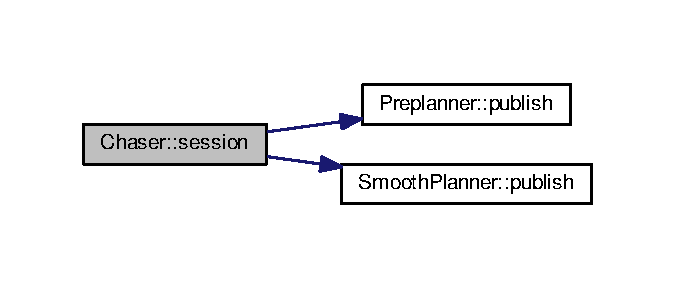
\includegraphics[width=324pt]{class_chaser_a7d736728bb5327acf0d334d7d4b1b844_cgraph}
\end{center}
\end{figure}




\subsection{Member Data Documentation}
\index{Chaser@{Chaser}!is\+\_\+complete\+\_\+chasing\+\_\+path@{is\+\_\+complete\+\_\+chasing\+\_\+path}}
\index{is\+\_\+complete\+\_\+chasing\+\_\+path@{is\+\_\+complete\+\_\+chasing\+\_\+path}!Chaser@{Chaser}}
\subsubsection[{\texorpdfstring{is\+\_\+complete\+\_\+chasing\+\_\+path}{is_complete_chasing_path}}]{\setlength{\rightskip}{0pt plus 5cm}bool Chaser\+::is\+\_\+complete\+\_\+chasing\+\_\+path}\hypertarget{class_chaser_a53af032471ad6bdc828c4eae78085813}{}\label{class_chaser_a53af032471ad6bdc828c4eae78085813}


Definition at line 18 of file Chaser.\+h.

\index{Chaser@{Chaser}!is\+\_\+log@{is\+\_\+log}}
\index{is\+\_\+log@{is\+\_\+log}!Chaser@{Chaser}}
\subsubsection[{\texorpdfstring{is\+\_\+log}{is_log}}]{\setlength{\rightskip}{0pt plus 5cm}bool Chaser\+::is\+\_\+log}\hypertarget{class_chaser_a33b880dd48d1d983001fa93ba1a1184f}{}\label{class_chaser_a33b880dd48d1d983001fa93ba1a1184f}


Definition at line 19 of file Chaser.\+h.

\index{Chaser@{Chaser}!log\+\_\+dir@{log\+\_\+dir}}
\index{log\+\_\+dir@{log\+\_\+dir}!Chaser@{Chaser}}
\subsubsection[{\texorpdfstring{log\+\_\+dir}{log_dir}}]{\setlength{\rightskip}{0pt plus 5cm}string Chaser\+::log\+\_\+dir}\hypertarget{class_chaser_a9d9ad4c7ca00bcda38d2bc809f3e7654}{}\label{class_chaser_a9d9ad4c7ca00bcda38d2bc809f3e7654}


Definition at line 20 of file Chaser.\+h.



The documentation for this class was generated from the following files\+:\begin{DoxyCompactItemize}
\item 
include/auto\+\_\+chaser/\hyperlink{_chaser_8h}{Chaser.\+h}\item 
src/auto\+\_\+chaser/\hyperlink{_chaser_8cpp}{Chaser.\+cpp}\end{DoxyCompactItemize}

\hypertarget{struct_field_params}{}\section{Field\+Params Struct Reference}
\label{struct_field_params}\index{Field\+Params@{Field\+Params}}


{\ttfamily \#include $<$Common.\+h$>$}

\subsection*{Public Attributes}
\begin{DoxyCompactItemize}
\item 
double \hyperlink{struct_field_params_ae702824fca4d3a4b4bbf4ac90084e3a7}{x0}
\item 
double \hyperlink{struct_field_params_ae9d400dadcfaaff44706adae06664c83}{y0}
\item 
double \hyperlink{struct_field_params_a51178f64cc93a37d6d8f774228c24a0f}{z0}
\item 
double \hyperlink{struct_field_params_a9738077907a76512e49cb284ee3f1949}{lx}
\item 
double \hyperlink{struct_field_params_afb39ded77b5714992e9b2f8c5d735d30}{ly}
\item 
double \hyperlink{struct_field_params_ae7532b58aed59f5b47233e57b67acc1a}{lz}
\item 
double \hyperlink{struct_field_params_a520406c76b3abf392401626bc2161370}{resolution}
\item 
double \hyperlink{struct_field_params_ae6eabaa6e593c9dbac48b2f96bea80ec}{ray\+\_\+stride\+\_\+res}
\end{DoxyCompactItemize}


\subsection{Detailed Description}


Definition at line 104 of file Common.\+h.



\subsection{Member Data Documentation}
\index{Field\+Params@{Field\+Params}!lx@{lx}}
\index{lx@{lx}!Field\+Params@{Field\+Params}}
\subsubsection[{\texorpdfstring{lx}{lx}}]{\setlength{\rightskip}{0pt plus 5cm}double Field\+Params\+::lx}\hypertarget{struct_field_params_a9738077907a76512e49cb284ee3f1949}{}\label{struct_field_params_a9738077907a76512e49cb284ee3f1949}


Definition at line 106 of file Common.\+h.

\index{Field\+Params@{Field\+Params}!ly@{ly}}
\index{ly@{ly}!Field\+Params@{Field\+Params}}
\subsubsection[{\texorpdfstring{ly}{ly}}]{\setlength{\rightskip}{0pt plus 5cm}double Field\+Params\+::ly}\hypertarget{struct_field_params_afb39ded77b5714992e9b2f8c5d735d30}{}\label{struct_field_params_afb39ded77b5714992e9b2f8c5d735d30}


Definition at line 106 of file Common.\+h.

\index{Field\+Params@{Field\+Params}!lz@{lz}}
\index{lz@{lz}!Field\+Params@{Field\+Params}}
\subsubsection[{\texorpdfstring{lz}{lz}}]{\setlength{\rightskip}{0pt plus 5cm}double Field\+Params\+::lz}\hypertarget{struct_field_params_ae7532b58aed59f5b47233e57b67acc1a}{}\label{struct_field_params_ae7532b58aed59f5b47233e57b67acc1a}


Definition at line 106 of file Common.\+h.

\index{Field\+Params@{Field\+Params}!ray\+\_\+stride\+\_\+res@{ray\+\_\+stride\+\_\+res}}
\index{ray\+\_\+stride\+\_\+res@{ray\+\_\+stride\+\_\+res}!Field\+Params@{Field\+Params}}
\subsubsection[{\texorpdfstring{ray\+\_\+stride\+\_\+res}{ray_stride_res}}]{\setlength{\rightskip}{0pt plus 5cm}double Field\+Params\+::ray\+\_\+stride\+\_\+res}\hypertarget{struct_field_params_ae6eabaa6e593c9dbac48b2f96bea80ec}{}\label{struct_field_params_ae6eabaa6e593c9dbac48b2f96bea80ec}


Definition at line 108 of file Common.\+h.

\index{Field\+Params@{Field\+Params}!resolution@{resolution}}
\index{resolution@{resolution}!Field\+Params@{Field\+Params}}
\subsubsection[{\texorpdfstring{resolution}{resolution}}]{\setlength{\rightskip}{0pt plus 5cm}double Field\+Params\+::resolution}\hypertarget{struct_field_params_a520406c76b3abf392401626bc2161370}{}\label{struct_field_params_a520406c76b3abf392401626bc2161370}


Definition at line 107 of file Common.\+h.

\index{Field\+Params@{Field\+Params}!x0@{x0}}
\index{x0@{x0}!Field\+Params@{Field\+Params}}
\subsubsection[{\texorpdfstring{x0}{x0}}]{\setlength{\rightskip}{0pt plus 5cm}double Field\+Params\+::x0}\hypertarget{struct_field_params_ae702824fca4d3a4b4bbf4ac90084e3a7}{}\label{struct_field_params_ae702824fca4d3a4b4bbf4ac90084e3a7}


Definition at line 105 of file Common.\+h.

\index{Field\+Params@{Field\+Params}!y0@{y0}}
\index{y0@{y0}!Field\+Params@{Field\+Params}}
\subsubsection[{\texorpdfstring{y0}{y0}}]{\setlength{\rightskip}{0pt plus 5cm}double Field\+Params\+::y0}\hypertarget{struct_field_params_ae9d400dadcfaaff44706adae06664c83}{}\label{struct_field_params_ae9d400dadcfaaff44706adae06664c83}


Definition at line 105 of file Common.\+h.

\index{Field\+Params@{Field\+Params}!z0@{z0}}
\index{z0@{z0}!Field\+Params@{Field\+Params}}
\subsubsection[{\texorpdfstring{z0}{z0}}]{\setlength{\rightskip}{0pt plus 5cm}double Field\+Params\+::z0}\hypertarget{struct_field_params_a51178f64cc93a37d6d8f774228c24a0f}{}\label{struct_field_params_a51178f64cc93a37d6d8f774228c24a0f}


Definition at line 105 of file Common.\+h.



The documentation for this struct was generated from the following file\+:\begin{DoxyCompactItemize}
\item 
include/auto\+\_\+chaser/\hyperlink{_common_8h}{Common.\+h}\end{DoxyCompactItemize}

\hypertarget{struct_grid_field}{}\section{Grid\+Field Struct Reference}
\label{struct_grid_field}\index{Grid\+Field@{Grid\+Field}}


{\ttfamily \#include $<$Common.\+h$>$}



Collaboration diagram for Grid\+Field\+:
\nopagebreak
\begin{figure}[H]
\begin{center}
\leavevmode
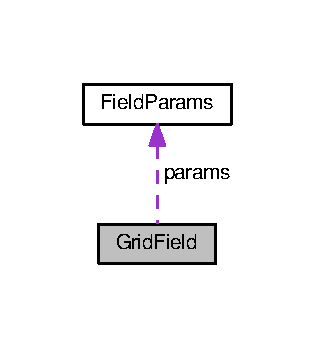
\includegraphics[width=152pt]{struct_grid_field__coll__graph}
\end{center}
\end{figure}
\subsection*{Public Member Functions}
\begin{DoxyCompactItemize}
\item 
\hyperlink{struct_grid_field_a1c755284583cf0070cb3dbed9b5fe925}{Grid\+Field} ()
\item 
\hyperlink{struct_grid_field_ad1542bce01b2a0f0a5860e20ced0e24d}{Grid\+Field} (\hyperlink{struct_field_params}{Field\+Params} param)
\item 
vector$<$ \hyperlink{struct_node}{Node}$<$ Point $>$ $>$ \hyperlink{struct_grid_field_acd8fd9f0893ad94aa4f20b4b4d81802a}{generate\+\_\+node} (int prefix)
\item 
void \hyperlink{struct_grid_field_aa50e5e42c9932e52be3d1d9a38ebf28b}{set\+Origin} (Point X0)
\item 
Point \hyperlink{struct_grid_field_ab0d5ba92ad35ab9b7bdd29506b6753de}{get\+Origin} ()
\item 
Point \hyperlink{struct_grid_field_aacd39f9388090694e5c428cc612fd887}{get\+Centre} ()
\item 
Point \hyperlink{struct_grid_field_ab1a81e68d9e761cfb901c726bd9b0518}{get\+Cell\+Pnt} (Vector3i idx)
\item 
float \hyperlink{struct_grid_field_a9b1f94c44fc47953c38b8e2fe815860d}{get\+Value} (Point pnt)
\item 
Vector3i \hyperlink{struct_grid_field_a1a70c2de6239c1b086d01dc89b161b7c}{get\+Cell\+Idx} (Point pnt)
\item 
vector$<$ Vector3i $>$ \hyperlink{struct_grid_field_a7827c27a1d3b08f930c7f828eef14f0d}{get\+Ray\+Idx} (Point pnt1, Point pnt2)
\item 
float \hyperlink{struct_grid_field_af9f5144af2f0cdb99784ea54c42a8516}{get\+Ray\+Min} (Point pnt1, Point pnt2, float clamping\+\_\+val)
\item 
float \hyperlink{struct_grid_field_a3e49ca50129cb18db833bd4168c5d254}{get\+Ray\+Mean} (Point pnt1, Point pnt2)
\item 
void \hyperlink{struct_grid_field_a5f9debacee6e66e30a30ad7e0759ff15}{update\+Cell} (Point pnt, float val)
\item 
void \hyperlink{struct_grid_field_aeec99711fdc1486528b34fddff21c33f}{update\+Cell} (Vector3i idx, float val)
\item 
int \hyperlink{struct_grid_field_ae838908e288e110c7d1d680fadc6b2ba}{get\+Num\+Cell} ()
\end{DoxyCompactItemize}
\subsection*{Public Attributes}
\begin{DoxyCompactItemize}
\item 
\hyperlink{struct_field_params}{Field\+Params} \hyperlink{struct_grid_field_a735e3033049d10f084e74083ae44dd21}{params}
\item 
Vector\+Xf \hyperlink{struct_grid_field_a14f0f8f41ce92d7e5ab4c539ef9bc495}{node\+\_\+xs}
\item 
Vector\+Xf \hyperlink{struct_grid_field_a07e209546d687dd58557871744f7a9a6}{node\+\_\+ys}
\item 
Vector\+Xf \hyperlink{struct_grid_field_ab97e893cedd450d502165bcb7e3ed7ca}{node\+\_\+zs}
\item 
vector$<$ Point $>$ \hyperlink{struct_grid_field_a76901c3a463e8cbe456c8f73bc264380}{pnts\+\_\+list}
\item 
int \hyperlink{struct_grid_field_a7777c8b5bf6db312fcceecdfd012c9ca}{Nx}
\item 
int \hyperlink{struct_grid_field_a4cc2cac3066c31f0e6af9745cf994674}{Ny}
\item 
int \hyperlink{struct_grid_field_ae624c780496411e632ca5581b84a6177}{Nz}
\item 
vector$<$ Point $>$ \hyperlink{struct_grid_field_ad5dc16fb46eef17df3a554f5b5604611}{saved\+\_\+points}
\item 
float $\ast$$\ast$$\ast$ \hyperlink{struct_grid_field_a46802a85d9533d4371d12597f0247c7d}{field\+\_\+vals}
\end{DoxyCompactItemize}


\subsection{Detailed Description}


Definition at line 137 of file Common.\+h.



\subsection{Constructor \& Destructor Documentation}
\index{Grid\+Field@{Grid\+Field}!Grid\+Field@{Grid\+Field}}
\index{Grid\+Field@{Grid\+Field}!Grid\+Field@{Grid\+Field}}
\subsubsection[{\texorpdfstring{Grid\+Field()}{GridField()}}]{\setlength{\rightskip}{0pt plus 5cm}Grid\+Field\+::\+Grid\+Field (
\begin{DoxyParamCaption}
{}
\end{DoxyParamCaption}
)}\hypertarget{struct_grid_field_a1c755284583cf0070cb3dbed9b5fe925}{}\label{struct_grid_field_a1c755284583cf0070cb3dbed9b5fe925}


Definition at line 90 of file Common.\+cpp.

\index{Grid\+Field@{Grid\+Field}!Grid\+Field@{Grid\+Field}}
\index{Grid\+Field@{Grid\+Field}!Grid\+Field@{Grid\+Field}}
\subsubsection[{\texorpdfstring{Grid\+Field(\+Field\+Params param)}{GridField(FieldParams param)}}]{\setlength{\rightskip}{0pt plus 5cm}Grid\+Field\+::\+Grid\+Field (
\begin{DoxyParamCaption}
\item[{{\bf Field\+Params}}]{param}
\end{DoxyParamCaption}
)}\hypertarget{struct_grid_field_ad1542bce01b2a0f0a5860e20ced0e24d}{}\label{struct_grid_field_ad1542bce01b2a0f0a5860e20ced0e24d}


Definition at line 91 of file Common.\+cpp.



\subsection{Member Function Documentation}
\index{Grid\+Field@{Grid\+Field}!generate\+\_\+node@{generate\+\_\+node}}
\index{generate\+\_\+node@{generate\+\_\+node}!Grid\+Field@{Grid\+Field}}
\subsubsection[{\texorpdfstring{generate\+\_\+node(int prefix)}{generate_node(int prefix)}}]{\setlength{\rightskip}{0pt plus 5cm}vector$<$ {\bf Node}$<$ Point $>$ $>$ Grid\+Field\+::generate\+\_\+node (
\begin{DoxyParamCaption}
\item[{int}]{prefix}
\end{DoxyParamCaption}
)}\hypertarget{struct_grid_field_acd8fd9f0893ad94aa4f20b4b4d81802a}{}\label{struct_grid_field_acd8fd9f0893ad94aa4f20b4b4d81802a}


Definition at line 137 of file Common.\+cpp.



Here is the caller graph for this function\+:
\nopagebreak
\begin{figure}[H]
\begin{center}
\leavevmode
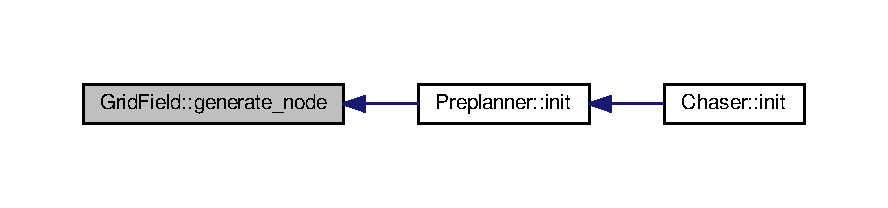
\includegraphics[width=350pt]{struct_grid_field_acd8fd9f0893ad94aa4f20b4b4d81802a_icgraph}
\end{center}
\end{figure}


\index{Grid\+Field@{Grid\+Field}!get\+Cell\+Idx@{get\+Cell\+Idx}}
\index{get\+Cell\+Idx@{get\+Cell\+Idx}!Grid\+Field@{Grid\+Field}}
\subsubsection[{\texorpdfstring{get\+Cell\+Idx(\+Point pnt)}{getCellIdx(Point pnt)}}]{\setlength{\rightskip}{0pt plus 5cm}Vector3i Grid\+Field\+::get\+Cell\+Idx (
\begin{DoxyParamCaption}
\item[{Point}]{pnt}
\end{DoxyParamCaption}
)}\hypertarget{struct_grid_field_a1a70c2de6239c1b086d01dc89b161b7c}{}\label{struct_grid_field_a1a70c2de6239c1b086d01dc89b161b7c}


Definition at line 205 of file Common.\+cpp.



Here is the caller graph for this function\+:
\nopagebreak
\begin{figure}[H]
\begin{center}
\leavevmode
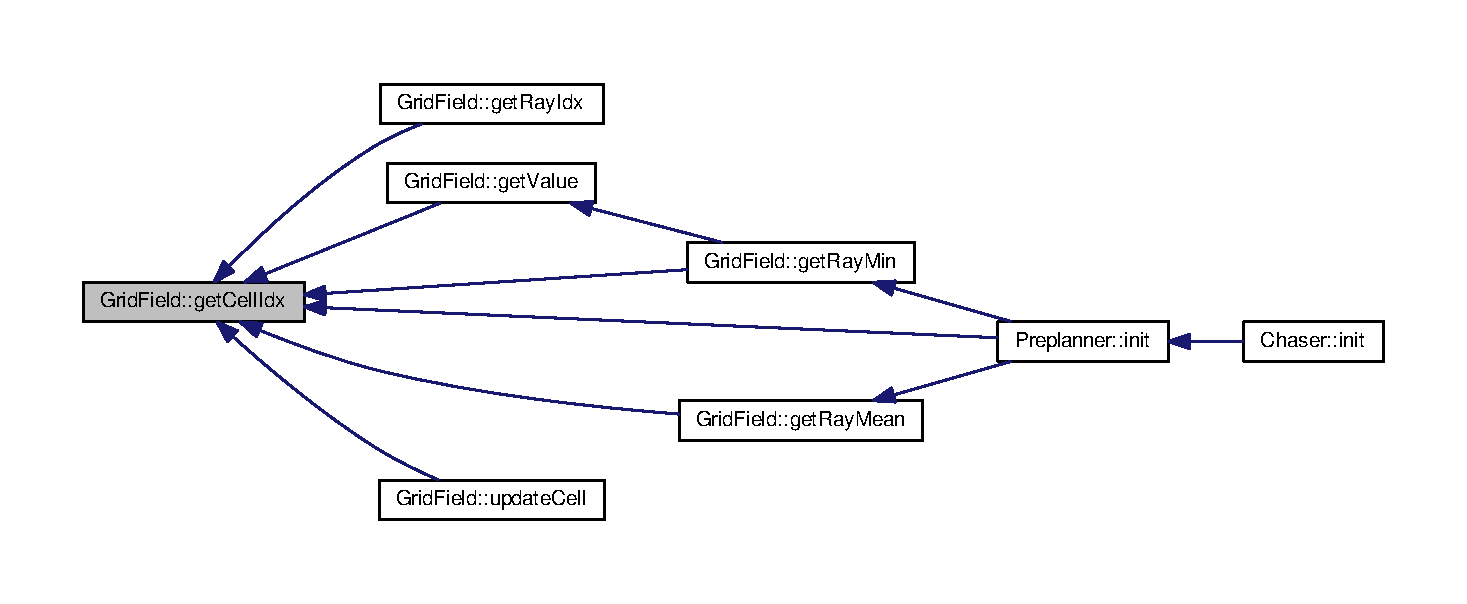
\includegraphics[width=350pt]{struct_grid_field_a1a70c2de6239c1b086d01dc89b161b7c_icgraph}
\end{center}
\end{figure}


\index{Grid\+Field@{Grid\+Field}!get\+Cell\+Pnt@{get\+Cell\+Pnt}}
\index{get\+Cell\+Pnt@{get\+Cell\+Pnt}!Grid\+Field@{Grid\+Field}}
\subsubsection[{\texorpdfstring{get\+Cell\+Pnt(\+Vector3i idx)}{getCellPnt(Vector3i idx)}}]{\setlength{\rightskip}{0pt plus 5cm}Point Grid\+Field\+::get\+Cell\+Pnt (
\begin{DoxyParamCaption}
\item[{Vector3i}]{idx}
\end{DoxyParamCaption}
)}\hypertarget{struct_grid_field_ab1a81e68d9e761cfb901c726bd9b0518}{}\label{struct_grid_field_ab1a81e68d9e761cfb901c726bd9b0518}


Definition at line 184 of file Common.\+cpp.

\index{Grid\+Field@{Grid\+Field}!get\+Centre@{get\+Centre}}
\index{get\+Centre@{get\+Centre}!Grid\+Field@{Grid\+Field}}
\subsubsection[{\texorpdfstring{get\+Centre()}{getCentre()}}]{\setlength{\rightskip}{0pt plus 5cm}Point Grid\+Field\+::get\+Centre (
\begin{DoxyParamCaption}
{}
\end{DoxyParamCaption}
)}\hypertarget{struct_grid_field_aacd39f9388090694e5c428cc612fd887}{}\label{struct_grid_field_aacd39f9388090694e5c428cc612fd887}


Definition at line 176 of file Common.\+cpp.



Here is the caller graph for this function\+:
\nopagebreak
\begin{figure}[H]
\begin{center}
\leavevmode
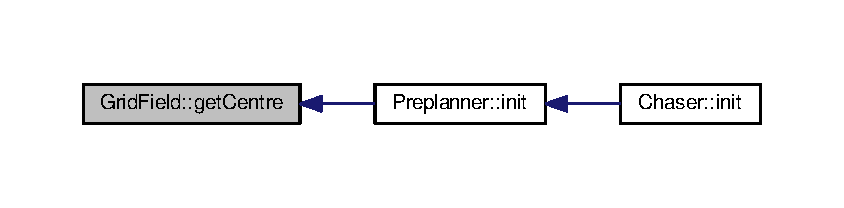
\includegraphics[width=350pt]{struct_grid_field_aacd39f9388090694e5c428cc612fd887_icgraph}
\end{center}
\end{figure}


\index{Grid\+Field@{Grid\+Field}!get\+Num\+Cell@{get\+Num\+Cell}}
\index{get\+Num\+Cell@{get\+Num\+Cell}!Grid\+Field@{Grid\+Field}}
\subsubsection[{\texorpdfstring{get\+Num\+Cell()}{getNumCell()}}]{\setlength{\rightskip}{0pt plus 5cm}int Grid\+Field\+::get\+Num\+Cell (
\begin{DoxyParamCaption}
{}
\end{DoxyParamCaption}
)\hspace{0.3cm}{\ttfamily [inline]}}\hypertarget{struct_grid_field_ae838908e288e110c7d1d680fadc6b2ba}{}\label{struct_grid_field_ae838908e288e110c7d1d680fadc6b2ba}


Definition at line 168 of file Common.\+h.

\index{Grid\+Field@{Grid\+Field}!get\+Origin@{get\+Origin}}
\index{get\+Origin@{get\+Origin}!Grid\+Field@{Grid\+Field}}
\subsubsection[{\texorpdfstring{get\+Origin()}{getOrigin()}}]{\setlength{\rightskip}{0pt plus 5cm}Point Grid\+Field\+::get\+Origin (
\begin{DoxyParamCaption}
{}
\end{DoxyParamCaption}
)}\hypertarget{struct_grid_field_ab0d5ba92ad35ab9b7bdd29506b6753de}{}\label{struct_grid_field_ab0d5ba92ad35ab9b7bdd29506b6753de}


Definition at line 167 of file Common.\+cpp.

\index{Grid\+Field@{Grid\+Field}!get\+Ray\+Idx@{get\+Ray\+Idx}}
\index{get\+Ray\+Idx@{get\+Ray\+Idx}!Grid\+Field@{Grid\+Field}}
\subsubsection[{\texorpdfstring{get\+Ray\+Idx(\+Point pnt1, Point pnt2)}{getRayIdx(Point pnt1, Point pnt2)}}]{\setlength{\rightskip}{0pt plus 5cm}vector$<$ Vector3i $>$ Grid\+Field\+::get\+Ray\+Idx (
\begin{DoxyParamCaption}
\item[{Point}]{pnt1, }
\item[{Point}]{pnt2}
\end{DoxyParamCaption}
)}\hypertarget{struct_grid_field_a7827c27a1d3b08f930c7f828eef14f0d}{}\label{struct_grid_field_a7827c27a1d3b08f930c7f828eef14f0d}


Definition at line 226 of file Common.\+cpp.



Here is the call graph for this function\+:
\nopagebreak
\begin{figure}[H]
\begin{center}
\leavevmode
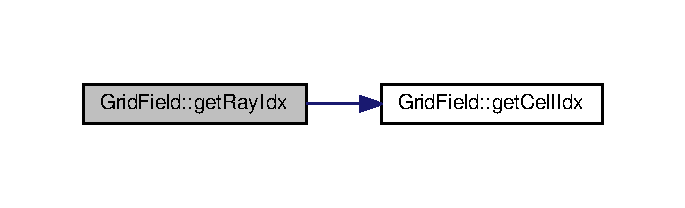
\includegraphics[width=329pt]{struct_grid_field_a7827c27a1d3b08f930c7f828eef14f0d_cgraph}
\end{center}
\end{figure}


\index{Grid\+Field@{Grid\+Field}!get\+Ray\+Mean@{get\+Ray\+Mean}}
\index{get\+Ray\+Mean@{get\+Ray\+Mean}!Grid\+Field@{Grid\+Field}}
\subsubsection[{\texorpdfstring{get\+Ray\+Mean(\+Point pnt1, Point pnt2)}{getRayMean(Point pnt1, Point pnt2)}}]{\setlength{\rightskip}{0pt plus 5cm}float Grid\+Field\+::get\+Ray\+Mean (
\begin{DoxyParamCaption}
\item[{Point}]{pnt1, }
\item[{Point}]{pnt2}
\end{DoxyParamCaption}
)}\hypertarget{struct_grid_field_a3e49ca50129cb18db833bd4168c5d254}{}\label{struct_grid_field_a3e49ca50129cb18db833bd4168c5d254}


Definition at line 303 of file Common.\+cpp.



Here is the call graph for this function\+:
\nopagebreak
\begin{figure}[H]
\begin{center}
\leavevmode
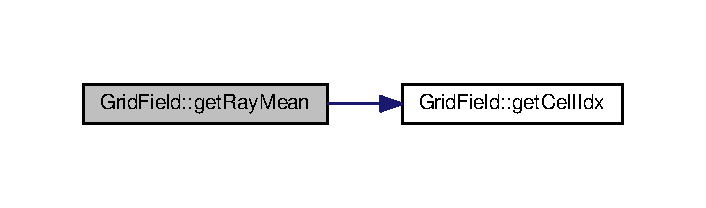
\includegraphics[width=339pt]{struct_grid_field_a3e49ca50129cb18db833bd4168c5d254_cgraph}
\end{center}
\end{figure}




Here is the caller graph for this function\+:
\nopagebreak
\begin{figure}[H]
\begin{center}
\leavevmode
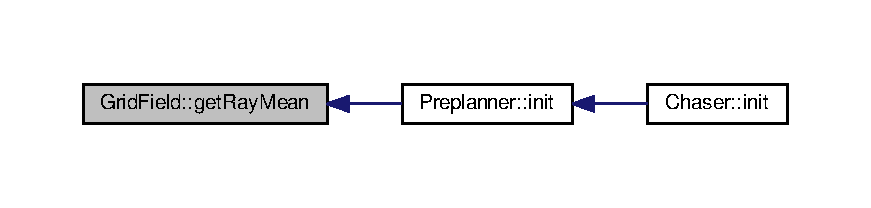
\includegraphics[width=350pt]{struct_grid_field_a3e49ca50129cb18db833bd4168c5d254_icgraph}
\end{center}
\end{figure}


\index{Grid\+Field@{Grid\+Field}!get\+Ray\+Min@{get\+Ray\+Min}}
\index{get\+Ray\+Min@{get\+Ray\+Min}!Grid\+Field@{Grid\+Field}}
\subsubsection[{\texorpdfstring{get\+Ray\+Min(\+Point pnt1, Point pnt2, float clamping\+\_\+val)}{getRayMin(Point pnt1, Point pnt2, float clamping_val)}}]{\setlength{\rightskip}{0pt plus 5cm}float Grid\+Field\+::get\+Ray\+Min (
\begin{DoxyParamCaption}
\item[{Point}]{pnt1, }
\item[{Point}]{pnt2, }
\item[{float}]{clamping\+\_\+val}
\end{DoxyParamCaption}
)}\hypertarget{struct_grid_field_af9f5144af2f0cdb99784ea54c42a8516}{}\label{struct_grid_field_af9f5144af2f0cdb99784ea54c42a8516}


Definition at line 259 of file Common.\+cpp.



Here is the call graph for this function\+:
\nopagebreak
\begin{figure}[H]
\begin{center}
\leavevmode
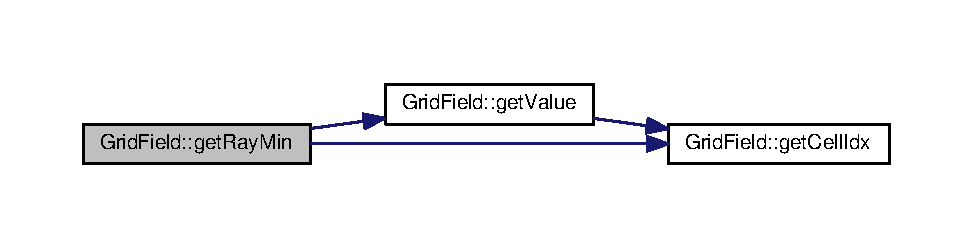
\includegraphics[width=350pt]{struct_grid_field_af9f5144af2f0cdb99784ea54c42a8516_cgraph}
\end{center}
\end{figure}




Here is the caller graph for this function\+:
\nopagebreak
\begin{figure}[H]
\begin{center}
\leavevmode
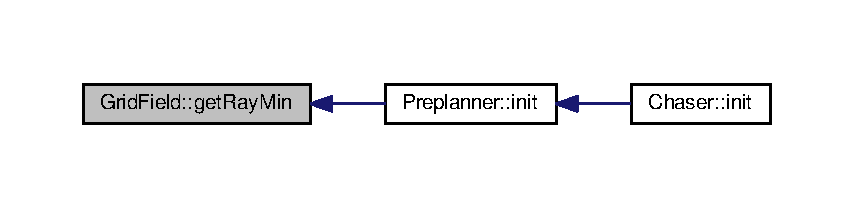
\includegraphics[width=350pt]{struct_grid_field_af9f5144af2f0cdb99784ea54c42a8516_icgraph}
\end{center}
\end{figure}


\index{Grid\+Field@{Grid\+Field}!get\+Value@{get\+Value}}
\index{get\+Value@{get\+Value}!Grid\+Field@{Grid\+Field}}
\subsubsection[{\texorpdfstring{get\+Value(\+Point pnt)}{getValue(Point pnt)}}]{\setlength{\rightskip}{0pt plus 5cm}float Grid\+Field\+::get\+Value (
\begin{DoxyParamCaption}
\item[{Point}]{pnt}
\end{DoxyParamCaption}
)}\hypertarget{struct_grid_field_a9b1f94c44fc47953c38b8e2fe815860d}{}\label{struct_grid_field_a9b1f94c44fc47953c38b8e2fe815860d}


Definition at line 253 of file Common.\+cpp.



Here is the call graph for this function\+:
\nopagebreak
\begin{figure}[H]
\begin{center}
\leavevmode
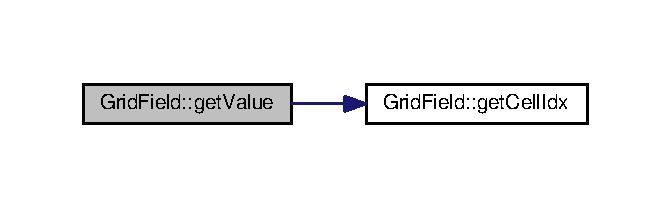
\includegraphics[width=322pt]{struct_grid_field_a9b1f94c44fc47953c38b8e2fe815860d_cgraph}
\end{center}
\end{figure}




Here is the caller graph for this function\+:
\nopagebreak
\begin{figure}[H]
\begin{center}
\leavevmode
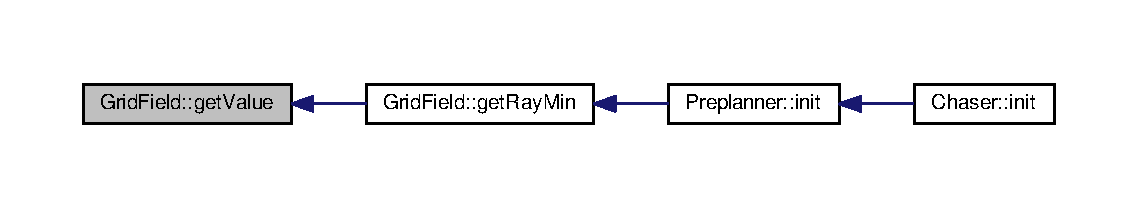
\includegraphics[width=350pt]{struct_grid_field_a9b1f94c44fc47953c38b8e2fe815860d_icgraph}
\end{center}
\end{figure}


\index{Grid\+Field@{Grid\+Field}!set\+Origin@{set\+Origin}}
\index{set\+Origin@{set\+Origin}!Grid\+Field@{Grid\+Field}}
\subsubsection[{\texorpdfstring{set\+Origin(\+Point X0)}{setOrigin(Point X0)}}]{\setlength{\rightskip}{0pt plus 5cm}void Grid\+Field\+::set\+Origin (
\begin{DoxyParamCaption}
\item[{Point}]{X0}
\end{DoxyParamCaption}
)}\hypertarget{struct_grid_field_aa50e5e42c9932e52be3d1d9a38ebf28b}{}\label{struct_grid_field_aa50e5e42c9932e52be3d1d9a38ebf28b}


Definition at line 155 of file Common.\+cpp.

\index{Grid\+Field@{Grid\+Field}!update\+Cell@{update\+Cell}}
\index{update\+Cell@{update\+Cell}!Grid\+Field@{Grid\+Field}}
\subsubsection[{\texorpdfstring{update\+Cell(\+Point pnt, float val)}{updateCell(Point pnt, float val)}}]{\setlength{\rightskip}{0pt plus 5cm}void Grid\+Field\+::update\+Cell (
\begin{DoxyParamCaption}
\item[{Point}]{pnt, }
\item[{float}]{val}
\end{DoxyParamCaption}
)}\hypertarget{struct_grid_field_a5f9debacee6e66e30a30ad7e0759ff15}{}\label{struct_grid_field_a5f9debacee6e66e30a30ad7e0759ff15}


Definition at line 347 of file Common.\+cpp.



Here is the call graph for this function\+:
\nopagebreak
\begin{figure}[H]
\begin{center}
\leavevmode
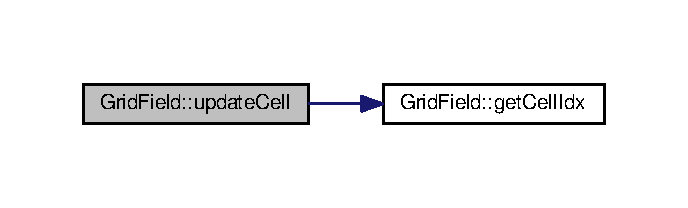
\includegraphics[width=330pt]{struct_grid_field_a5f9debacee6e66e30a30ad7e0759ff15_cgraph}
\end{center}
\end{figure}


\index{Grid\+Field@{Grid\+Field}!update\+Cell@{update\+Cell}}
\index{update\+Cell@{update\+Cell}!Grid\+Field@{Grid\+Field}}
\subsubsection[{\texorpdfstring{update\+Cell(\+Vector3i idx, float val)}{updateCell(Vector3i idx, float val)}}]{\setlength{\rightskip}{0pt plus 5cm}void Grid\+Field\+::update\+Cell (
\begin{DoxyParamCaption}
\item[{Vector3i}]{idx, }
\item[{float}]{val}
\end{DoxyParamCaption}
)}\hypertarget{struct_grid_field_aeec99711fdc1486528b34fddff21c33f}{}\label{struct_grid_field_aeec99711fdc1486528b34fddff21c33f}


Definition at line 356 of file Common.\+cpp.



\subsection{Member Data Documentation}
\index{Grid\+Field@{Grid\+Field}!field\+\_\+vals@{field\+\_\+vals}}
\index{field\+\_\+vals@{field\+\_\+vals}!Grid\+Field@{Grid\+Field}}
\subsubsection[{\texorpdfstring{field\+\_\+vals}{field_vals}}]{\setlength{\rightskip}{0pt plus 5cm}float$\ast$$\ast$$\ast$ Grid\+Field\+::field\+\_\+vals}\hypertarget{struct_grid_field_a46802a85d9533d4371d12597f0247c7d}{}\label{struct_grid_field_a46802a85d9533d4371d12597f0247c7d}


Definition at line 143 of file Common.\+h.

\index{Grid\+Field@{Grid\+Field}!node\+\_\+xs@{node\+\_\+xs}}
\index{node\+\_\+xs@{node\+\_\+xs}!Grid\+Field@{Grid\+Field}}
\subsubsection[{\texorpdfstring{node\+\_\+xs}{node_xs}}]{\setlength{\rightskip}{0pt plus 5cm}Vector\+Xf Grid\+Field\+::node\+\_\+xs}\hypertarget{struct_grid_field_a14f0f8f41ce92d7e5ab4c539ef9bc495}{}\label{struct_grid_field_a14f0f8f41ce92d7e5ab4c539ef9bc495}


Definition at line 139 of file Common.\+h.

\index{Grid\+Field@{Grid\+Field}!node\+\_\+ys@{node\+\_\+ys}}
\index{node\+\_\+ys@{node\+\_\+ys}!Grid\+Field@{Grid\+Field}}
\subsubsection[{\texorpdfstring{node\+\_\+ys}{node_ys}}]{\setlength{\rightskip}{0pt plus 5cm}Vector\+Xf Grid\+Field\+::node\+\_\+ys}\hypertarget{struct_grid_field_a07e209546d687dd58557871744f7a9a6}{}\label{struct_grid_field_a07e209546d687dd58557871744f7a9a6}


Definition at line 139 of file Common.\+h.

\index{Grid\+Field@{Grid\+Field}!node\+\_\+zs@{node\+\_\+zs}}
\index{node\+\_\+zs@{node\+\_\+zs}!Grid\+Field@{Grid\+Field}}
\subsubsection[{\texorpdfstring{node\+\_\+zs}{node_zs}}]{\setlength{\rightskip}{0pt plus 5cm}Vector\+Xf Grid\+Field\+::node\+\_\+zs}\hypertarget{struct_grid_field_ab97e893cedd450d502165bcb7e3ed7ca}{}\label{struct_grid_field_ab97e893cedd450d502165bcb7e3ed7ca}


Definition at line 139 of file Common.\+h.

\index{Grid\+Field@{Grid\+Field}!Nx@{Nx}}
\index{Nx@{Nx}!Grid\+Field@{Grid\+Field}}
\subsubsection[{\texorpdfstring{Nx}{Nx}}]{\setlength{\rightskip}{0pt plus 5cm}int Grid\+Field\+::\+Nx}\hypertarget{struct_grid_field_a7777c8b5bf6db312fcceecdfd012c9ca}{}\label{struct_grid_field_a7777c8b5bf6db312fcceecdfd012c9ca}


Definition at line 141 of file Common.\+h.

\index{Grid\+Field@{Grid\+Field}!Ny@{Ny}}
\index{Ny@{Ny}!Grid\+Field@{Grid\+Field}}
\subsubsection[{\texorpdfstring{Ny}{Ny}}]{\setlength{\rightskip}{0pt plus 5cm}int Grid\+Field\+::\+Ny}\hypertarget{struct_grid_field_a4cc2cac3066c31f0e6af9745cf994674}{}\label{struct_grid_field_a4cc2cac3066c31f0e6af9745cf994674}


Definition at line 141 of file Common.\+h.

\index{Grid\+Field@{Grid\+Field}!Nz@{Nz}}
\index{Nz@{Nz}!Grid\+Field@{Grid\+Field}}
\subsubsection[{\texorpdfstring{Nz}{Nz}}]{\setlength{\rightskip}{0pt plus 5cm}int Grid\+Field\+::\+Nz}\hypertarget{struct_grid_field_ae624c780496411e632ca5581b84a6177}{}\label{struct_grid_field_ae624c780496411e632ca5581b84a6177}


Definition at line 141 of file Common.\+h.

\index{Grid\+Field@{Grid\+Field}!params@{params}}
\index{params@{params}!Grid\+Field@{Grid\+Field}}
\subsubsection[{\texorpdfstring{params}{params}}]{\setlength{\rightskip}{0pt plus 5cm}{\bf Field\+Params} Grid\+Field\+::params}\hypertarget{struct_grid_field_a735e3033049d10f084e74083ae44dd21}{}\label{struct_grid_field_a735e3033049d10f084e74083ae44dd21}


Definition at line 138 of file Common.\+h.

\index{Grid\+Field@{Grid\+Field}!pnts\+\_\+list@{pnts\+\_\+list}}
\index{pnts\+\_\+list@{pnts\+\_\+list}!Grid\+Field@{Grid\+Field}}
\subsubsection[{\texorpdfstring{pnts\+\_\+list}{pnts_list}}]{\setlength{\rightskip}{0pt plus 5cm}vector$<$Point$>$ Grid\+Field\+::pnts\+\_\+list}\hypertarget{struct_grid_field_a76901c3a463e8cbe456c8f73bc264380}{}\label{struct_grid_field_a76901c3a463e8cbe456c8f73bc264380}


Definition at line 140 of file Common.\+h.

\index{Grid\+Field@{Grid\+Field}!saved\+\_\+points@{saved\+\_\+points}}
\index{saved\+\_\+points@{saved\+\_\+points}!Grid\+Field@{Grid\+Field}}
\subsubsection[{\texorpdfstring{saved\+\_\+points}{saved_points}}]{\setlength{\rightskip}{0pt plus 5cm}vector$<$Point$>$ Grid\+Field\+::saved\+\_\+points}\hypertarget{struct_grid_field_ad5dc16fb46eef17df3a554f5b5604611}{}\label{struct_grid_field_ad5dc16fb46eef17df3a554f5b5604611}


Definition at line 142 of file Common.\+h.



The documentation for this struct was generated from the following files\+:\begin{DoxyCompactItemize}
\item 
include/auto\+\_\+chaser/\hyperlink{_common_8h}{Common.\+h}\item 
src/auto\+\_\+chaser/\hyperlink{_common_8cpp}{Common.\+cpp}\end{DoxyCompactItemize}

\hypertarget{class_ui_1_1_main_window}{}\section{Ui\+:\+:Main\+Window Class Reference}
\label{class_ui_1_1_main_window}\index{Ui\+::\+Main\+Window@{Ui\+::\+Main\+Window}}


{\ttfamily \#include $<$ui\+\_\+mainwindow.\+h$>$}



Inheritance diagram for Ui\+:\+:Main\+Window\+:\nopagebreak
\begin{figure}[H]
\begin{center}
\leavevmode
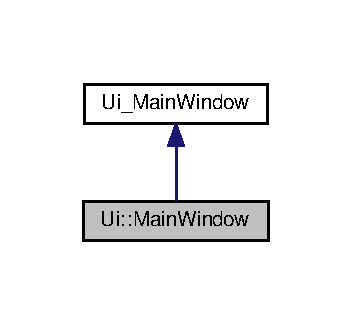
\includegraphics[width=169pt]{class_ui_1_1_main_window__inherit__graph}
\end{center}
\end{figure}


Collaboration diagram for Ui\+:\+:Main\+Window\+:\nopagebreak
\begin{figure}[H]
\begin{center}
\leavevmode
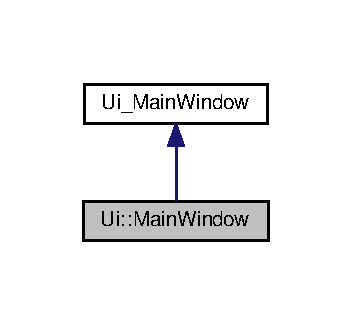
\includegraphics[width=169pt]{class_ui_1_1_main_window__coll__graph}
\end{center}
\end{figure}
\subsection*{Additional Inherited Members}


\subsection{Detailed Description}


The documentation for this class was generated from the following file\+:\begin{DoxyCompactItemize}
\item 
/home/jbs/catkin\+\_\+ws/src/traj\+\_\+gen\+\_\+vis\+\_\+developing/src/build-\/qt\+\_\+ui-\/\+Desktop-\/\+Debug/\hyperlink{ui__mainwindow_8h}{ui\+\_\+mainwindow.\+h}\end{DoxyCompactItemize}

\hypertarget{class_main_window}{}\section{Main\+Window Class Reference}
\label{class_main_window}\index{Main\+Window@{Main\+Window}}


{\ttfamily \#include $<$mainwindow.\+h$>$}



Inheritance diagram for Main\+Window\+:\nopagebreak
\begin{figure}[H]
\begin{center}
\leavevmode
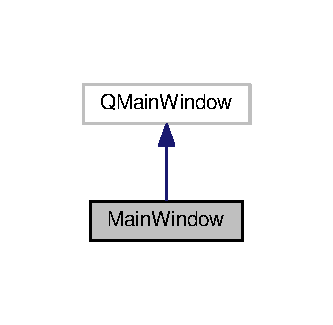
\includegraphics[width=160pt]{class_main_window__inherit__graph}
\end{center}
\end{figure}


Collaboration diagram for Main\+Window\+:
\nopagebreak
\begin{figure}[H]
\begin{center}
\leavevmode
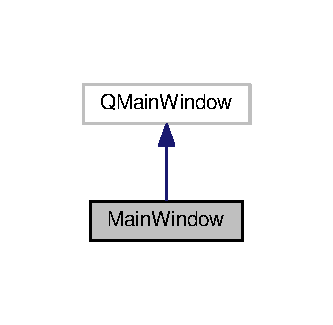
\includegraphics[width=350pt]{class_main_window__coll__graph}
\end{center}
\end{figure}
\subsection*{Public Member Functions}
\begin{DoxyCompactItemize}
\item 
\hyperlink{class_main_window_a6f0a90213d93b861d43c09dd01c52962}{Main\+Window} (\hyperlink{class_q_node}{Q\+Node} $\ast$\hyperlink{class_main_window_ac9d45be6e40fe6917339119e15c1b120}{qnode}, Q\+Widget $\ast$parent=0)
\item 
\hyperlink{class_main_window_ae98d00a93bc118200eeef9f9bba1dba7}{$\sim$\+Main\+Window} ()
\item 
void \hyperlink{class_main_window_a4e20a4a065fbb0e4d3532a45a0a91425}{close\+Event} (Q\+Close\+Event $\ast$event)
\item 
void \hyperlink{class_main_window_a4abba2c52f756524c0f388d0d3e6d6ec}{Read\+Settings} ()
\item 
void \hyperlink{class_main_window_a56a5e4d5e0a022e8c1ecf350d2916ade}{Write\+Settings} ()
\end{DoxyCompactItemize}
\subsection*{Private Slots}
\begin{DoxyCompactItemize}
\item 
void \hyperlink{class_main_window_a996e7b8e246db04a9931ea8c058eedf8}{on\+\_\+push\+Button\+\_\+chaser\+\_\+clicked} ()
\item 
void \hyperlink{class_main_window_a9aebdb686fc8f44bc84454443b094ef7}{on\+\_\+push\+Button\+\_\+ros\+\_\+clicked} ()
\item 
void \hyperlink{class_main_window_a543d311321e5dcb7a42384dd67c6bff4}{on\+\_\+push\+Button\+\_\+waypoint\+\_\+clicked} ()
\item 
void \hyperlink{class_main_window_a3cdeb477328d4aaeac315f62c632a4f2}{on\+\_\+push\+Button\+\_\+trajectory\+\_\+clicked} ()
\item 
void \hyperlink{class_main_window_aec26150ce3a1688a40230b79b088921d}{on\+\_\+push\+Button\+\_\+simulation\+\_\+clicked} ()
\item 
void \hyperlink{class_main_window_a5f2b259d7c85d5d32c1207a34d8b9af4}{on\+\_\+push\+Button\+\_\+save\+\_\+clicked} ()
\item 
void \hyperlink{class_main_window_a9c676468f012e842cd443d8029f8a242}{on\+\_\+push\+Button\+\_\+load\+\_\+clicked} ()
\item 
void \hyperlink{class_main_window_af777763ec745a8eeffe3f9925005fac1}{on\+\_\+push\+Button\+\_\+clear\+\_\+clicked} ()
\item 
void \hyperlink{class_main_window_a41e769472d468772dd3851cbd20ca9fb}{on\+\_\+push\+Button\+\_\+undo\+\_\+clicked} ()
\item 
void \hyperlink{class_main_window_a00ace1276164789fa5383e80ecbf8c6f}{on\+\_\+push\+Button\+\_\+one\+\_\+shot\+\_\+clicked} ()
\item 
void \hyperlink{class_main_window_a4513ffcd68256d01c44fa2602d4c6880}{text\+Edit\+\_\+write} (Q\+String)
\end{DoxyCompactItemize}
\subsection*{Private Attributes}
\begin{DoxyCompactItemize}
\item 
\hyperlink{class_ui_1_1_main_window}{Ui\+::\+Main\+Window} $\ast$ \hyperlink{class_main_window_a35466a70ed47252a0191168126a352a5}{ui}
\item 
\hyperlink{class_q_node}{Q\+Node} $\ast$ \hyperlink{class_main_window_ac9d45be6e40fe6917339119e15c1b120}{qnode}
\end{DoxyCompactItemize}


\subsection{Detailed Description}


\subsection{Constructor \& Destructor Documentation}
\index{Main\+Window@{Main\+Window}!Main\+Window@{Main\+Window}}
\index{Main\+Window@{Main\+Window}!Main\+Window@{Main\+Window}}
\subsubsection[{\texorpdfstring{Main\+Window(\+Q\+Node $\ast$qnode, Q\+Widget $\ast$parent=0)}{MainWindow(QNode *qnode, QWidget *parent=0)}}]{\setlength{\rightskip}{0pt plus 5cm}Main\+Window\+::\+Main\+Window (
\begin{DoxyParamCaption}
\item[{{\bf Q\+Node} $\ast$}]{qnode, }
\item[{Q\+Widget $\ast$}]{parent = {\ttfamily 0}}
\end{DoxyParamCaption}
)\hspace{0.3cm}{\ttfamily [explicit]}}\hypertarget{class_main_window_a6f0a90213d93b861d43c09dd01c52962}{}\label{class_main_window_a6f0a90213d93b861d43c09dd01c52962}

\begin{DoxyCode}
5                                                    :
6     QMainWindow(parent),\hyperlink{class_main_window_ac9d45be6e40fe6917339119e15c1b120}{qnode}(qnode),
7     \hyperlink{class_main_window_a35466a70ed47252a0191168126a352a5}{ui}(\textcolor{keyword}{new} \hyperlink{class_ui_1_1_main_window}{Ui::MainWindow})
8 \{
9     \hyperlink{class_main_window_a35466a70ed47252a0191168126a352a5}{ui}->\hyperlink{class_ui___main_window_acf4a0872c4c77d8f43a2ec66ed849b58}{setupUi}(\textcolor{keyword}{this});
10 
11 
12     \textcolor{comment}{// intial configuration}
13 
14     \textcolor{comment}{// logos}
15     \textcolor{keywordtype}{string} cd = \_\_FILE\_\_;
16     cd.erase(cd.end()-14,cd.end());
17     cout<<\textcolor{stringliteral}{"current directory: "}<<cd<<endl;
18 
19     QPixmap pix\_larr((cd + \textcolor{stringliteral}{"/resources/LARR.jpg"}).c\_str());
20     \textcolor{keywordtype}{int} w = \hyperlink{class_main_window_a35466a70ed47252a0191168126a352a5}{ui}->\hyperlink{class_ui___main_window_a32587f1e879f5b685d375d2daa20f7a6}{label\_larr}->width();
21     \textcolor{keywordtype}{int} h = \hyperlink{class_main_window_a35466a70ed47252a0191168126a352a5}{ui}->\hyperlink{class_ui___main_window_a32587f1e879f5b685d375d2daa20f7a6}{label\_larr}->height();
22     \hyperlink{class_main_window_a35466a70ed47252a0191168126a352a5}{ui}->\hyperlink{class_ui___main_window_a32587f1e879f5b685d375d2daa20f7a6}{label\_larr}->setPixmap(pix\_larr.scaled(w,h,Qt::KeepAspectRatio));
23 
24     QPixmap pix\_larr2((cd +\textcolor{stringliteral}{"/resources/maxresdefault.jpg"}).c\_str());
25     \textcolor{keywordtype}{int} w2 = \hyperlink{class_main_window_a35466a70ed47252a0191168126a352a5}{ui}->\hyperlink{class_ui___main_window_a06fc1a01ac3ba3d4d1f75a0e8ab06684}{label\_larr2}->width();
26     \textcolor{keywordtype}{int} h2 = \hyperlink{class_main_window_a35466a70ed47252a0191168126a352a5}{ui}->\hyperlink{class_ui___main_window_a06fc1a01ac3ba3d4d1f75a0e8ab06684}{label\_larr2}->height();
27     \hyperlink{class_main_window_a35466a70ed47252a0191168126a352a5}{ui}->\hyperlink{class_ui___main_window_a06fc1a01ac3ba3d4d1f75a0e8ab06684}{label\_larr2}->setPixmap(pix\_larr2.scaled(w2,h2,Qt::KeepAspectRatio));
28 
29     \textcolor{comment}{// checkable }
30     \hyperlink{class_main_window_a35466a70ed47252a0191168126a352a5}{ui}->\hyperlink{class_ui___main_window_afd109ead0ad1ae7ae67ad1df803c9c38}{pushButton\_simulation}->setStyleSheet(\textcolor{stringliteral}{"QPushButton:checked\{background-color:
       rgba(100, 20, 20,50); \}"});
31     
32     QObject::connect(qnode, SIGNAL(rosShutdown()), \textcolor{keyword}{this}, SLOT(close()));
33     QObject::connect(qnode,SIGNAL(writeOnBoard(QString)),\textcolor{keyword}{this},SLOT(
      \hyperlink{class_main_window_a4513ffcd68256d01c44fa2602d4c6880}{textEdit\_write}(QString)));
34 
35     \textcolor{comment}{// load settings }
36     \hyperlink{class_main_window_a4abba2c52f756524c0f388d0d3e6d6ec}{ReadSettings}();
37 
38 \}
\end{DoxyCode}
\index{Main\+Window@{Main\+Window}!````~Main\+Window@{$\sim$\+Main\+Window}}
\index{````~Main\+Window@{$\sim$\+Main\+Window}!Main\+Window@{Main\+Window}}
\subsubsection[{\texorpdfstring{$\sim$\+Main\+Window()}{~MainWindow()}}]{\setlength{\rightskip}{0pt plus 5cm}Main\+Window\+::$\sim$\+Main\+Window (
\begin{DoxyParamCaption}
{}
\end{DoxyParamCaption}
)}\hypertarget{class_main_window_ae98d00a93bc118200eeef9f9bba1dba7}{}\label{class_main_window_ae98d00a93bc118200eeef9f9bba1dba7}

\begin{DoxyCode}
41 \{
42     \textcolor{keyword}{delete} \hyperlink{class_main_window_a35466a70ed47252a0191168126a352a5}{ui};
43 \}
\end{DoxyCode}


\subsection{Member Function Documentation}
\index{Main\+Window@{Main\+Window}!close\+Event@{close\+Event}}
\index{close\+Event@{close\+Event}!Main\+Window@{Main\+Window}}
\subsubsection[{\texorpdfstring{close\+Event(\+Q\+Close\+Event $\ast$event)}{closeEvent(QCloseEvent *event)}}]{\setlength{\rightskip}{0pt plus 5cm}void Main\+Window\+::close\+Event (
\begin{DoxyParamCaption}
\item[{Q\+Close\+Event $\ast$}]{event}
\end{DoxyParamCaption}
)}\hypertarget{class_main_window_a4e20a4a065fbb0e4d3532a45a0a91425}{}\label{class_main_window_a4e20a4a065fbb0e4d3532a45a0a91425}

\begin{DoxyCode}
234                                              \{
235 
236         \hyperlink{class_main_window_ac9d45be6e40fe6917339119e15c1b120}{qnode}->\hyperlink{class_q_node_a770568addece696138f515d38408ff5c}{shutdown}();
237         \hyperlink{class_main_window_a56a5e4d5e0a022e8c1ecf350d2916ade}{WriteSettings}();
238         QMainWindow::closeEvent(event);
239 \}
\end{DoxyCode}
\index{Main\+Window@{Main\+Window}!on\+\_\+push\+Button\+\_\+chaser\+\_\+clicked@{on\+\_\+push\+Button\+\_\+chaser\+\_\+clicked}}
\index{on\+\_\+push\+Button\+\_\+chaser\+\_\+clicked@{on\+\_\+push\+Button\+\_\+chaser\+\_\+clicked}!Main\+Window@{Main\+Window}}
\subsubsection[{\texorpdfstring{on\+\_\+push\+Button\+\_\+chaser\+\_\+clicked}{on_pushButton_chaser_clicked}}]{\setlength{\rightskip}{0pt plus 5cm}void Main\+Window\+::on\+\_\+push\+Button\+\_\+chaser\+\_\+clicked (
\begin{DoxyParamCaption}
{}
\end{DoxyParamCaption}
)\hspace{0.3cm}{\ttfamily [private]}, {\ttfamily [slot]}}\hypertarget{class_main_window_a996e7b8e246db04a9931ea8c058eedf8}{}\label{class_main_window_a996e7b8e246db04a9931ea8c058eedf8}

\begin{DoxyCode}
70                                              \{
71 
72     \textcolor{keywordflow}{if}(\hyperlink{class_main_window_a35466a70ed47252a0191168126a352a5}{ui}->\hyperlink{class_ui___main_window_a9e8499b7c9a9717499abde993da72ed5}{pushButton\_chaser}->isChecked())\{      
73         \hyperlink{class_main_window_ac9d45be6e40fe6917339119e15c1b120}{qnode}->\hyperlink{class_q_node_ad2d828488fb632a008c7d3ee0e1d1fa2}{chaser\_wrapper}.\hyperlink{class_wrapper_a8cddd5ffbaeb5ab0b5d8d8d0c74f810f}{objects\_handler}.
      \hyperlink{class_objects_handler_acaefe98eb412d4c32cda2bf0bd602ae7}{is\_insert\_permit} = \textcolor{keyword}{true};  
74         \hyperlink{class_main_window_a35466a70ed47252a0191168126a352a5}{ui}->\hyperlink{class_ui___main_window_af13441b9fd874f1aeb2ec5cefaeb0bce}{textEdit\_board}->append(\textcolor{stringliteral}{"please select chaser init pose: /chaser\_init\_pose"});
75     \}\textcolor{keywordflow}{else}\{
76         \hyperlink{class_main_window_a35466a70ed47252a0191168126a352a5}{ui}->\hyperlink{class_ui___main_window_af13441b9fd874f1aeb2ec5cefaeb0bce}{textEdit\_board}->append(\textcolor{stringliteral}{"finishing chaser spawning selection"});
77         \hyperlink{class_main_window_ac9d45be6e40fe6917339119e15c1b120}{qnode}->\hyperlink{class_q_node_ad2d828488fb632a008c7d3ee0e1d1fa2}{chaser\_wrapper}.\hyperlink{class_wrapper_a8cddd5ffbaeb5ab0b5d8d8d0c74f810f}{objects\_handler}.
      \hyperlink{class_objects_handler_acaefe98eb412d4c32cda2bf0bd602ae7}{is\_insert\_permit} = \textcolor{keyword}{false};  
78 
79     \}
80 
81 \}
\end{DoxyCode}
\index{Main\+Window@{Main\+Window}!on\+\_\+push\+Button\+\_\+clear\+\_\+clicked@{on\+\_\+push\+Button\+\_\+clear\+\_\+clicked}}
\index{on\+\_\+push\+Button\+\_\+clear\+\_\+clicked@{on\+\_\+push\+Button\+\_\+clear\+\_\+clicked}!Main\+Window@{Main\+Window}}
\subsubsection[{\texorpdfstring{on\+\_\+push\+Button\+\_\+clear\+\_\+clicked}{on_pushButton_clear_clicked}}]{\setlength{\rightskip}{0pt plus 5cm}void Main\+Window\+::on\+\_\+push\+Button\+\_\+clear\+\_\+clicked (
\begin{DoxyParamCaption}
{}
\end{DoxyParamCaption}
)\hspace{0.3cm}{\ttfamily [private]}, {\ttfamily [slot]}}\hypertarget{class_main_window_af777763ec745a8eeffe3f9925005fac1}{}\label{class_main_window_af777763ec745a8eeffe3f9925005fac1}

\begin{DoxyCode}
181 \{
182     \hyperlink{class_main_window_ac9d45be6e40fe6917339119e15c1b120}{qnode}->\hyperlink{class_q_node_adc66765125dfd755d5e7f0c0eb6e6395}{target\_manager}.\hyperlink{class_target_manager_a13242c4a8b96b97cfeddea19aabc1181}{clear\_waypoint}();
183 \}
\end{DoxyCode}
\index{Main\+Window@{Main\+Window}!on\+\_\+push\+Button\+\_\+load\+\_\+clicked@{on\+\_\+push\+Button\+\_\+load\+\_\+clicked}}
\index{on\+\_\+push\+Button\+\_\+load\+\_\+clicked@{on\+\_\+push\+Button\+\_\+load\+\_\+clicked}!Main\+Window@{Main\+Window}}
\subsubsection[{\texorpdfstring{on\+\_\+push\+Button\+\_\+load\+\_\+clicked}{on_pushButton_load_clicked}}]{\setlength{\rightskip}{0pt plus 5cm}void Main\+Window\+::on\+\_\+push\+Button\+\_\+load\+\_\+clicked (
\begin{DoxyParamCaption}
{}
\end{DoxyParamCaption}
)\hspace{0.3cm}{\ttfamily [private]}, {\ttfamily [slot]}}\hypertarget{class_main_window_a9c676468f012e842cd443d8029f8a242}{}\label{class_main_window_a9c676468f012e842cd443d8029f8a242}

\begin{DoxyCode}
137 \{
138     \textcolor{comment}{// file read : queue wil be filled with these}
139 
140     \textcolor{keywordtype}{string} filename = \hyperlink{class_main_window_a35466a70ed47252a0191168126a352a5}{ui}->\hyperlink{class_ui___main_window_a4a75bfb754049f89fccef822cad712d6}{lineEdit\_target\_trajectory}->text().toStdString();
141     std::ifstream infile;
142     infile.open(filename);
143     \textcolor{keywordflow}{if}(infile.is\_open())
144         \hyperlink{class_main_window_a35466a70ed47252a0191168126a352a5}{ui}->\hyperlink{class_ui___main_window_af13441b9fd874f1aeb2ec5cefaeb0bce}{textEdit\_board}->append(QString(\textcolor{stringliteral}{"pnts reading.."}));
145     \textcolor{keywordflow}{else}
146     \{
147         \hyperlink{class_main_window_a35466a70ed47252a0191168126a352a5}{ui}->\hyperlink{class_ui___main_window_af13441b9fd874f1aeb2ec5cefaeb0bce}{textEdit\_board}->append(QString(\textcolor{stringliteral}{"could not open file."}));
148         \textcolor{keywordflow}{return};
149     \}
150 
151     std::vector<geometry\_msgs::PoseStamped> queue\_replace;
152 
153     \textcolor{keywordflow}{while} (! infile.eof())\{
154         std::string line;
155         getline(infile, line); \textcolor{comment}{// if no delimiter given, new line is that}
156         \textcolor{comment}{// std::cout<<line<<std::endl;}
157         std::stringstream stream(line);
158         std::string val;
159         \textcolor{keywordtype}{int} xyz\_idx = 0;
160         geometry\_msgs::PoseStamped wpnt;
161 
162         \textcolor{keywordflow}{while}(! stream.eof()) \{
163             getline(stream, val, \textcolor{charliteral}{','});
164             \textcolor{keywordflow}{if}(xyz\_idx == 0)
165                 wpnt.pose.position.x = atof(val.c\_str());
166             \textcolor{keywordflow}{else} \textcolor{keywordflow}{if}(xyz\_idx == 1)
167                 wpnt.pose.position.y = atof(val.c\_str());
168             \textcolor{keywordflow}{else}
169                 wpnt.pose.position.z = atof(val.c\_str());
170             xyz\_idx ++;
171         \}
172         queue\_replace.push\_back(wpnt);
173         \textcolor{comment}{// std::cout<< wpnt.pose.position.x <<" , "<< wpnt.pose.position.y <<" ,
       "<<wpnt.pose.position.z<<std::endl;}
174     \}
175 
176     queue\_replace.pop\_back();
177     \hyperlink{class_main_window_ac9d45be6e40fe6917339119e15c1b120}{qnode}->\hyperlink{class_q_node_adc66765125dfd755d5e7f0c0eb6e6395}{target\_manager}.\hyperlink{class_target_manager_a8b96689879cecac3d9109914eb6230ef}{queue\_file\_load}(queue\_replace);
178 \}
\end{DoxyCode}
\index{Main\+Window@{Main\+Window}!on\+\_\+push\+Button\+\_\+one\+\_\+shot\+\_\+clicked@{on\+\_\+push\+Button\+\_\+one\+\_\+shot\+\_\+clicked}}
\index{on\+\_\+push\+Button\+\_\+one\+\_\+shot\+\_\+clicked@{on\+\_\+push\+Button\+\_\+one\+\_\+shot\+\_\+clicked}!Main\+Window@{Main\+Window}}
\subsubsection[{\texorpdfstring{on\+\_\+push\+Button\+\_\+one\+\_\+shot\+\_\+clicked}{on_pushButton_one_shot_clicked}}]{\setlength{\rightskip}{0pt plus 5cm}void Main\+Window\+::on\+\_\+push\+Button\+\_\+one\+\_\+shot\+\_\+clicked (
\begin{DoxyParamCaption}
{}
\end{DoxyParamCaption}
)\hspace{0.3cm}{\ttfamily [private]}, {\ttfamily [slot]}}\hypertarget{class_main_window_a00ace1276164789fa5383e80ecbf8c6f}{}\label{class_main_window_a00ace1276164789fa5383e80ecbf8c6f}

\begin{DoxyCode}
190                                                \{
191     \hyperlink{class_main_window_a35466a70ed47252a0191168126a352a5}{ui}->\hyperlink{class_ui___main_window_af13441b9fd874f1aeb2ec5cefaeb0bce}{textEdit\_board}->append(\textcolor{stringliteral}{"one shot simulatoin requested."});
192     \textcolor{keywordtype}{double} tf = atoi(\hyperlink{class_main_window_a35466a70ed47252a0191168126a352a5}{ui}->\hyperlink{class_ui___main_window_afc0d94ce5096c619c413cfae9b62014c}{lineEdit\_tf}->text().toStdString().c\_str());    
193     \textcolor{keywordflow}{if} (\hyperlink{class_main_window_ac9d45be6e40fe6917339119e15c1b120}{qnode}->\hyperlink{class_q_node_a65f0fc9f27f336150f33b53a7c51d80b}{trigger\_one\_shot}(tf))
194         \hyperlink{class_main_window_a35466a70ed47252a0191168126a352a5}{ui}->\hyperlink{class_ui___main_window_af13441b9fd874f1aeb2ec5cefaeb0bce}{textEdit\_board}->append(\textcolor{stringliteral}{"chasing path obtained"});
195     \textcolor{keywordflow}{else} 
196         \hyperlink{class_main_window_a35466a70ed47252a0191168126a352a5}{ui}->\hyperlink{class_ui___main_window_af13441b9fd874f1aeb2ec5cefaeb0bce}{textEdit\_board}->append(\textcolor{stringliteral}{"chasing failed"});    
197 \};
\end{DoxyCode}
\index{Main\+Window@{Main\+Window}!on\+\_\+push\+Button\+\_\+ros\+\_\+clicked@{on\+\_\+push\+Button\+\_\+ros\+\_\+clicked}}
\index{on\+\_\+push\+Button\+\_\+ros\+\_\+clicked@{on\+\_\+push\+Button\+\_\+ros\+\_\+clicked}!Main\+Window@{Main\+Window}}
\subsubsection[{\texorpdfstring{on\+\_\+push\+Button\+\_\+ros\+\_\+clicked}{on_pushButton_ros_clicked}}]{\setlength{\rightskip}{0pt plus 5cm}void Main\+Window\+::on\+\_\+push\+Button\+\_\+ros\+\_\+clicked (
\begin{DoxyParamCaption}
{}
\end{DoxyParamCaption}
)\hspace{0.3cm}{\ttfamily [private]}, {\ttfamily [slot]}}\hypertarget{class_main_window_a9aebdb686fc8f44bc84454443b094ef7}{}\label{class_main_window_a9aebdb686fc8f44bc84454443b094ef7}

\begin{DoxyCode}
46 \{
47     \textcolor{keywordflow}{if}(\hyperlink{class_main_window_ac9d45be6e40fe6917339119e15c1b120}{qnode}->\hyperlink{class_q_node_a32d00dbcf15c277e08caabf95af04f6e}{on\_init}())\{
48         \hyperlink{class_main_window_a35466a70ed47252a0191168126a352a5}{ui}->\hyperlink{class_ui___main_window_af13441b9fd874f1aeb2ec5cefaeb0bce}{textEdit\_board}->append(\textcolor{stringliteral}{"ros connected."});
49         \hyperlink{class_main_window_ac9d45be6e40fe6917339119e15c1b120}{qnode}->\hyperlink{class_q_node_a98b08e7704b00df8648f8c08dffe950c}{is\_connected} = \textcolor{keyword}{true};
50 
51     \}\textcolor{keywordflow}{else}\{
52         \hyperlink{class_main_window_a35466a70ed47252a0191168126a352a5}{ui}->\hyperlink{class_ui___main_window_af13441b9fd874f1aeb2ec5cefaeb0bce}{textEdit\_board}->append(\textcolor{stringliteral}{"failed. retry"});
53     \}
54 \}
\end{DoxyCode}
\index{Main\+Window@{Main\+Window}!on\+\_\+push\+Button\+\_\+save\+\_\+clicked@{on\+\_\+push\+Button\+\_\+save\+\_\+clicked}}
\index{on\+\_\+push\+Button\+\_\+save\+\_\+clicked@{on\+\_\+push\+Button\+\_\+save\+\_\+clicked}!Main\+Window@{Main\+Window}}
\subsubsection[{\texorpdfstring{on\+\_\+push\+Button\+\_\+save\+\_\+clicked}{on_pushButton_save_clicked}}]{\setlength{\rightskip}{0pt plus 5cm}void Main\+Window\+::on\+\_\+push\+Button\+\_\+save\+\_\+clicked (
\begin{DoxyParamCaption}
{}
\end{DoxyParamCaption}
)\hspace{0.3cm}{\ttfamily [private]}, {\ttfamily [slot]}}\hypertarget{class_main_window_a5f2b259d7c85d5d32c1207a34d8b9af4}{}\label{class_main_window_a5f2b259d7c85d5d32c1207a34d8b9af4}

\begin{DoxyCode}
115 \{
116 
117     \textcolor{comment}{// file write}
118     std::ofstream wnpt\_file;
119     \textcolor{keywordtype}{string} filename = \hyperlink{class_main_window_a35466a70ed47252a0191168126a352a5}{ui}->\hyperlink{class_ui___main_window_a4a75bfb754049f89fccef822cad712d6}{lineEdit\_target\_trajectory}->text().toStdString();
120     wnpt\_file.open(filename);
121 
122     \textcolor{keywordflow}{if}(wnpt\_file.is\_open())\{
123         \textcolor{keywordflow}{for}(\textcolor{keyword}{auto} it = \hyperlink{class_main_window_ac9d45be6e40fe6917339119e15c1b120}{qnode}->\hyperlink{class_q_node_adc66765125dfd755d5e7f0c0eb6e6395}{target\_manager}.\hyperlink{class_target_manager_a0bbcb1981504e3bc587c3a98f41a91e9}{queue}.begin();it<
      \hyperlink{class_main_window_ac9d45be6e40fe6917339119e15c1b120}{qnode}->\hyperlink{class_q_node_adc66765125dfd755d5e7f0c0eb6e6395}{target\_manager}.\hyperlink{class_target_manager_a0bbcb1981504e3bc587c3a98f41a91e9}{queue}.end();it++)\{
124             wnpt\_file<<std::to\_string(it->pose.position.x)<<\textcolor{stringliteral}{","}<<std::to\_string(it->pose.position.y)<<\textcolor{stringliteral}{","}<<
      std::to\_string(it->pose.position.z)<<\textcolor{stringliteral}{"\(\backslash\)n"};
125         \}
126         wnpt\_file.close();
127 
128         
129         \hyperlink{class_main_window_a35466a70ed47252a0191168126a352a5}{ui}->\hyperlink{class_ui___main_window_af13441b9fd874f1aeb2ec5cefaeb0bce}{textEdit\_board}->append(QString((\textcolor{keywordtype}{string}(\textcolor{stringliteral}{"to "}) + 
      \hyperlink{_common_8h_a7770cb36d4f4c6e78ff68516ecb2123c}{GetCurrentWorkingDir}()+\textcolor{stringliteral}{"/"} + filename + \textcolor{keywordtype}{string}(\textcolor{stringliteral}{", written"})).data()));
130 
131     \}\textcolor{keywordflow}{else}
132         \hyperlink{class_main_window_a35466a70ed47252a0191168126a352a5}{ui}->\hyperlink{class_ui___main_window_af13441b9fd874f1aeb2ec5cefaeb0bce}{textEdit\_board}->append(QString(\textcolor{stringliteral}{"file not written."}));
133 
134 \}
\end{DoxyCode}
\index{Main\+Window@{Main\+Window}!on\+\_\+push\+Button\+\_\+simulation\+\_\+clicked@{on\+\_\+push\+Button\+\_\+simulation\+\_\+clicked}}
\index{on\+\_\+push\+Button\+\_\+simulation\+\_\+clicked@{on\+\_\+push\+Button\+\_\+simulation\+\_\+clicked}!Main\+Window@{Main\+Window}}
\subsubsection[{\texorpdfstring{on\+\_\+push\+Button\+\_\+simulation\+\_\+clicked}{on_pushButton_simulation_clicked}}]{\setlength{\rightskip}{0pt plus 5cm}void Main\+Window\+::on\+\_\+push\+Button\+\_\+simulation\+\_\+clicked (
\begin{DoxyParamCaption}
{}
\end{DoxyParamCaption}
)\hspace{0.3cm}{\ttfamily [private]}, {\ttfamily [slot]}}\hypertarget{class_main_window_aec26150ce3a1688a40230b79b088921d}{}\label{class_main_window_aec26150ce3a1688a40230b79b088921d}

\begin{DoxyCode}
94 \{
95     \textcolor{keywordflow}{if}(\hyperlink{class_main_window_a35466a70ed47252a0191168126a352a5}{ui}->\hyperlink{class_ui___main_window_afd109ead0ad1ae7ae67ad1df803c9c38}{pushButton\_simulation}->isChecked())\{ 
96 
97         \textcolor{keywordflow}{if}(\hyperlink{class_main_window_ac9d45be6e40fe6917339119e15c1b120}{qnode}->\hyperlink{class_q_node_ad2d828488fb632a008c7d3ee0e1d1fa2}{chaser\_wrapper}.\hyperlink{class_wrapper_a8cddd5ffbaeb5ab0b5d8d8d0c74f810f}{objects\_handler}.
      \hyperlink{class_objects_handler_a16165ae7c0167ba8d2a0151a8a4fbfd5}{is\_chaser\_spawned} and \hyperlink{class_main_window_ac9d45be6e40fe6917339119e15c1b120}{qnode}->\hyperlink{class_q_node_adc66765125dfd755d5e7f0c0eb6e6395}{target\_manager}.
      \hyperlink{class_target_manager_a507af7ce1ac562510c1b907553a2e596}{is\_path})\{
98             \hyperlink{class_main_window_a35466a70ed47252a0191168126a352a5}{ui}->\hyperlink{class_ui___main_window_af13441b9fd874f1aeb2ec5cefaeb0bce}{textEdit\_board}->append(\textcolor{stringliteral}{"move target.."});
99             \textcolor{comment}{// simulation end time }
100             \hyperlink{class_main_window_ac9d45be6e40fe6917339119e15c1b120}{qnode}->\hyperlink{class_q_node_a7a127726e48aa5bde733d715af7a744c}{simulation\_end\_time} = atof(\hyperlink{class_main_window_a35466a70ed47252a0191168126a352a5}{ui}->
      \hyperlink{class_ui___main_window_afc0d94ce5096c619c413cfae9b62014c}{lineEdit\_tf}->text().toStdString().c\_str());
101             \hyperlink{class_main_window_ac9d45be6e40fe6917339119e15c1b120}{qnode}->\hyperlink{class_q_node_a6ace2d0aa89adecfe699b3f1c3ce0b0f}{is\_in\_session} = \textcolor{keyword}{true};
102             \hyperlink{class_main_window_ac9d45be6e40fe6917339119e15c1b120}{qnode}->\hyperlink{class_q_node_a96e6599c14732ded065ae6a5b004f872}{button\_click\_time} = ros::Time::now();        
103         \}
104         \textcolor{keywordflow}{else}\{
105             \hyperlink{class_main_window_a35466a70ed47252a0191168126a352a5}{ui}->\hyperlink{class_ui___main_window_af13441b9fd874f1aeb2ec5cefaeb0bce}{textEdit\_board}->append(\textcolor{stringliteral}{"target path not obtained or no chaser spawned."});
106         \}
107     \}\textcolor{keywordflow}{else}\{
108         \hyperlink{class_main_window_a35466a70ed47252a0191168126a352a5}{ui}->\hyperlink{class_ui___main_window_af13441b9fd874f1aeb2ec5cefaeb0bce}{textEdit\_board}->append(\textcolor{stringliteral}{"stop target."});
109         \hyperlink{class_main_window_ac9d45be6e40fe6917339119e15c1b120}{qnode}->\hyperlink{class_q_node_a6ace2d0aa89adecfe699b3f1c3ce0b0f}{is\_in\_session} = \textcolor{keyword}{false};
110         \hyperlink{class_main_window_ac9d45be6e40fe6917339119e15c1b120}{qnode}->\hyperlink{class_q_node_a4b5f0a40821fbb176de620cb5a3921f7}{previous\_elapsed} = (ros::Time::now() - \hyperlink{class_main_window_ac9d45be6e40fe6917339119e15c1b120}{qnode}->
      \hyperlink{class_q_node_a96e6599c14732ded065ae6a5b004f872}{button\_click\_time}).toSec() + \hyperlink{class_main_window_ac9d45be6e40fe6917339119e15c1b120}{qnode}->\hyperlink{class_q_node_a4b5f0a40821fbb176de620cb5a3921f7}{previous\_elapsed}; \textcolor{comment}{// total
       elasped time}
111     \}
112 \}
\end{DoxyCode}
\index{Main\+Window@{Main\+Window}!on\+\_\+push\+Button\+\_\+trajectory\+\_\+clicked@{on\+\_\+push\+Button\+\_\+trajectory\+\_\+clicked}}
\index{on\+\_\+push\+Button\+\_\+trajectory\+\_\+clicked@{on\+\_\+push\+Button\+\_\+trajectory\+\_\+clicked}!Main\+Window@{Main\+Window}}
\subsubsection[{\texorpdfstring{on\+\_\+push\+Button\+\_\+trajectory\+\_\+clicked}{on_pushButton_trajectory_clicked}}]{\setlength{\rightskip}{0pt plus 5cm}void Main\+Window\+::on\+\_\+push\+Button\+\_\+trajectory\+\_\+clicked (
\begin{DoxyParamCaption}
{}
\end{DoxyParamCaption}
)\hspace{0.3cm}{\ttfamily [private]}, {\ttfamily [slot]}}\hypertarget{class_main_window_a3cdeb477328d4aaeac315f62c632a4f2}{}\label{class_main_window_a3cdeb477328d4aaeac315f62c632a4f2}

\begin{DoxyCode}
84 \{
85     
86     \textcolor{keywordtype}{double} tf = atof(\hyperlink{class_main_window_a35466a70ed47252a0191168126a352a5}{ui}->\hyperlink{class_ui___main_window_afc0d94ce5096c619c413cfae9b62014c}{lineEdit\_tf}->text().toStdString().c\_str());
87     \textcolor{keywordflow}{if}(\hyperlink{class_main_window_ac9d45be6e40fe6917339119e15c1b120}{qnode}->\hyperlink{class_q_node_adc66765125dfd755d5e7f0c0eb6e6395}{target\_manager}.\hyperlink{class_target_manager_a1c0e48d7a623e8b7caa11c6b1832956b}{global\_path\_generate}(tf))
88         \hyperlink{class_main_window_a4513ffcd68256d01c44fa2602d4c6880}{textEdit\_write}(\textcolor{stringliteral}{"target trajectory obtainted"});
89     \textcolor{keywordflow}{else}
90         \hyperlink{class_main_window_a4513ffcd68256d01c44fa2602d4c6880}{textEdit\_write}(\textcolor{stringliteral}{"target trajectory failed"});    
91 \}
\end{DoxyCode}
\index{Main\+Window@{Main\+Window}!on\+\_\+push\+Button\+\_\+undo\+\_\+clicked@{on\+\_\+push\+Button\+\_\+undo\+\_\+clicked}}
\index{on\+\_\+push\+Button\+\_\+undo\+\_\+clicked@{on\+\_\+push\+Button\+\_\+undo\+\_\+clicked}!Main\+Window@{Main\+Window}}
\subsubsection[{\texorpdfstring{on\+\_\+push\+Button\+\_\+undo\+\_\+clicked}{on_pushButton_undo_clicked}}]{\setlength{\rightskip}{0pt plus 5cm}void Main\+Window\+::on\+\_\+push\+Button\+\_\+undo\+\_\+clicked (
\begin{DoxyParamCaption}
{}
\end{DoxyParamCaption}
)\hspace{0.3cm}{\ttfamily [private]}, {\ttfamily [slot]}}\hypertarget{class_main_window_a41e769472d468772dd3851cbd20ca9fb}{}\label{class_main_window_a41e769472d468772dd3851cbd20ca9fb}

\begin{DoxyCode}
186 \{
187     \hyperlink{class_main_window_ac9d45be6e40fe6917339119e15c1b120}{qnode}->\hyperlink{class_q_node_adc66765125dfd755d5e7f0c0eb6e6395}{target\_manager}.\hyperlink{class_target_manager_af362d78ae6b0cc0a3ea288b2c138f482}{pop\_waypoint}();
188 \};
\end{DoxyCode}
\index{Main\+Window@{Main\+Window}!on\+\_\+push\+Button\+\_\+waypoint\+\_\+clicked@{on\+\_\+push\+Button\+\_\+waypoint\+\_\+clicked}}
\index{on\+\_\+push\+Button\+\_\+waypoint\+\_\+clicked@{on\+\_\+push\+Button\+\_\+waypoint\+\_\+clicked}!Main\+Window@{Main\+Window}}
\subsubsection[{\texorpdfstring{on\+\_\+push\+Button\+\_\+waypoint\+\_\+clicked}{on_pushButton_waypoint_clicked}}]{\setlength{\rightskip}{0pt plus 5cm}void Main\+Window\+::on\+\_\+push\+Button\+\_\+waypoint\+\_\+clicked (
\begin{DoxyParamCaption}
{}
\end{DoxyParamCaption}
)\hspace{0.3cm}{\ttfamily [private]}, {\ttfamily [slot]}}\hypertarget{class_main_window_a543d311321e5dcb7a42384dd67c6bff4}{}\label{class_main_window_a543d311321e5dcb7a42384dd67c6bff4}

\begin{DoxyCode}
57 \{
58     \textcolor{keywordflow}{if}(\hyperlink{class_main_window_a35466a70ed47252a0191168126a352a5}{ui}->\hyperlink{class_ui___main_window_a6b5d7c0f96cdb3276a33746fbcd7e8c7}{pushButton\_waypoint}->isChecked())\{        
59         \hyperlink{class_main_window_a35466a70ed47252a0191168126a352a5}{ui}->\hyperlink{class_ui___main_window_af13441b9fd874f1aeb2ec5cefaeb0bce}{textEdit\_board}->append(\textcolor{stringliteral}{"please select waypoints : /target\_waypoints "});
60         \hyperlink{class_main_window_ac9d45be6e40fe6917339119e15c1b120}{qnode}->\hyperlink{class_q_node_adc66765125dfd755d5e7f0c0eb6e6395}{target\_manager}.\hyperlink{class_target_manager_adf8a01c0942c3aac0445403d8f0f4cce}{is\_insert\_permit} = \textcolor{keyword}{true};
61 
62     \}\textcolor{keywordflow}{else}\{
63 
64         \hyperlink{class_main_window_a35466a70ed47252a0191168126a352a5}{ui}->\hyperlink{class_ui___main_window_af13441b9fd874f1aeb2ec5cefaeb0bce}{textEdit\_board}->append(\textcolor{stringliteral}{"finishing waypoints selection"});
65         \hyperlink{class_main_window_ac9d45be6e40fe6917339119e15c1b120}{qnode}->\hyperlink{class_q_node_adc66765125dfd755d5e7f0c0eb6e6395}{target\_manager}.\hyperlink{class_target_manager_adf8a01c0942c3aac0445403d8f0f4cce}{is\_insert\_permit} = \textcolor{keyword}{false};
66     \}
67 
68 \}
\end{DoxyCode}
\index{Main\+Window@{Main\+Window}!Read\+Settings@{Read\+Settings}}
\index{Read\+Settings@{Read\+Settings}!Main\+Window@{Main\+Window}}
\subsubsection[{\texorpdfstring{Read\+Settings()}{ReadSettings()}}]{\setlength{\rightskip}{0pt plus 5cm}void Main\+Window\+::\+Read\+Settings (
\begin{DoxyParamCaption}
{}
\end{DoxyParamCaption}
)}\hypertarget{class_main_window_a4abba2c52f756524c0f388d0d3e6d6ec}{}\label{class_main_window_a4abba2c52f756524c0f388d0d3e6d6ec}

\begin{DoxyCode}
204                              \{
205     QSettings settings(\textcolor{stringliteral}{"auto\_chaser"}, \hyperlink{class_main_window_ac9d45be6e40fe6917339119e15c1b120}{qnode}->\hyperlink{class_q_node_ac21ae24311df97ac0e15c97179763b0e}{nodeName}().c\_str());
206 
207     \textcolor{comment}{// setting names    }
208     QString filename\_logging = settings.value(\textcolor{stringliteral}{"filename\_logging"},QString(\textcolor{stringliteral}{"path\_saved.txt"})).toString();
209     QString filename\_waypoints = settings.value(\textcolor{stringliteral}{"filename\_waypoints"},QString(\textcolor{stringliteral}{"path\_saved.txt"})).toString();
210     QString simulation\_tf = settings.value(\textcolor{stringliteral}{"tf"}, QString(\textcolor{stringliteral}{"20"})).toString();
211 
212     
213     \textcolor{comment}{// fill with previous settings }
214     \hyperlink{class_main_window_a35466a70ed47252a0191168126a352a5}{ui}->\hyperlink{class_ui___main_window_a7ab71242b81ef9d13f83c16f6328f35d}{lineEdit\_logging\_dir}->setText(filename\_logging);
215     \hyperlink{class_main_window_a35466a70ed47252a0191168126a352a5}{ui}->\hyperlink{class_ui___main_window_afc0d94ce5096c619c413cfae9b62014c}{lineEdit\_tf}->setText(simulation\_tf);
216     \hyperlink{class_main_window_a35466a70ed47252a0191168126a352a5}{ui}->\hyperlink{class_ui___main_window_a4a75bfb754049f89fccef822cad712d6}{lineEdit\_target\_trajectory}->setText(filename\_waypoints);
217     
218 \}
\end{DoxyCode}
\index{Main\+Window@{Main\+Window}!text\+Edit\+\_\+write@{text\+Edit\+\_\+write}}
\index{text\+Edit\+\_\+write@{text\+Edit\+\_\+write}!Main\+Window@{Main\+Window}}
\subsubsection[{\texorpdfstring{text\+Edit\+\_\+write}{textEdit_write}}]{\setlength{\rightskip}{0pt plus 5cm}void Main\+Window\+::text\+Edit\+\_\+write (
\begin{DoxyParamCaption}
\item[{Q\+String}]{line}
\end{DoxyParamCaption}
)\hspace{0.3cm}{\ttfamily [private]}, {\ttfamily [slot]}}\hypertarget{class_main_window_a4513ffcd68256d01c44fa2602d4c6880}{}\label{class_main_window_a4513ffcd68256d01c44fa2602d4c6880}

\begin{DoxyCode}
199                                            \{    
200     \hyperlink{class_main_window_a35466a70ed47252a0191168126a352a5}{ui}->\hyperlink{class_ui___main_window_af13441b9fd874f1aeb2ec5cefaeb0bce}{textEdit\_board}->append(line);
201 \};
\end{DoxyCode}
\index{Main\+Window@{Main\+Window}!Write\+Settings@{Write\+Settings}}
\index{Write\+Settings@{Write\+Settings}!Main\+Window@{Main\+Window}}
\subsubsection[{\texorpdfstring{Write\+Settings()}{WriteSettings()}}]{\setlength{\rightskip}{0pt plus 5cm}void Main\+Window\+::\+Write\+Settings (
\begin{DoxyParamCaption}
{}
\end{DoxyParamCaption}
)}\hypertarget{class_main_window_a56a5e4d5e0a022e8c1ecf350d2916ade}{}\label{class_main_window_a56a5e4d5e0a022e8c1ecf350d2916ade}

\begin{DoxyCode}
220                               \{
221 
222     QSettings settings(\textcolor{stringliteral}{"auto\_chaser"}, \hyperlink{class_main_window_ac9d45be6e40fe6917339119e15c1b120}{qnode}->\hyperlink{class_q_node_ac21ae24311df97ac0e15c97179763b0e}{nodeName}().c\_str());
223     
224     settings.setValue(\textcolor{stringliteral}{"geometry"}, geometry());
225     settings.setValue(\textcolor{stringliteral}{"windowState"}, saveState());
226 
227     settings.setValue(\textcolor{stringliteral}{"filename\_logging"},\hyperlink{class_main_window_a35466a70ed47252a0191168126a352a5}{ui}->\hyperlink{class_ui___main_window_a7ab71242b81ef9d13f83c16f6328f35d}{lineEdit\_logging\_dir}->text());
228     settings.setValue(\textcolor{stringliteral}{"tf"},\hyperlink{class_main_window_a35466a70ed47252a0191168126a352a5}{ui}->\hyperlink{class_ui___main_window_afc0d94ce5096c619c413cfae9b62014c}{lineEdit\_tf}->text());
229     settings.setValue(\textcolor{stringliteral}{"filename\_waypoints"},\hyperlink{class_main_window_a35466a70ed47252a0191168126a352a5}{ui}->\hyperlink{class_ui___main_window_a4a75bfb754049f89fccef822cad712d6}{lineEdit\_target\_trajectory}->text
      ());
230 
231 
232 \}
\end{DoxyCode}


\subsection{Member Data Documentation}
\index{Main\+Window@{Main\+Window}!qnode@{qnode}}
\index{qnode@{qnode}!Main\+Window@{Main\+Window}}
\subsubsection[{\texorpdfstring{qnode}{qnode}}]{\setlength{\rightskip}{0pt plus 5cm}{\bf Q\+Node}$\ast$ Main\+Window\+::qnode\hspace{0.3cm}{\ttfamily [private]}}\hypertarget{class_main_window_ac9d45be6e40fe6917339119e15c1b120}{}\label{class_main_window_ac9d45be6e40fe6917339119e15c1b120}
\index{Main\+Window@{Main\+Window}!ui@{ui}}
\index{ui@{ui}!Main\+Window@{Main\+Window}}
\subsubsection[{\texorpdfstring{ui}{ui}}]{\setlength{\rightskip}{0pt plus 5cm}{\bf Ui\+::\+Main\+Window}$\ast$ Main\+Window\+::ui\hspace{0.3cm}{\ttfamily [private]}}\hypertarget{class_main_window_a35466a70ed47252a0191168126a352a5}{}\label{class_main_window_a35466a70ed47252a0191168126a352a5}


The documentation for this class was generated from the following files\+:\begin{DoxyCompactItemize}
\item 
/home/jbs/catkin\+\_\+ws/src/traj\+\_\+gen\+\_\+vis\+\_\+developing/src/qt\+\_\+ui/\hyperlink{mainwindow_8h}{mainwindow.\+h}\item 
/home/jbs/catkin\+\_\+ws/src/traj\+\_\+gen\+\_\+vis\+\_\+developing/src/qt\+\_\+ui/\hyperlink{mainwindow_8cpp}{mainwindow.\+cpp}\end{DoxyCompactItemize}

\hypertarget{struct_node}{}\section{Node$<$ T $>$ Struct Template Reference}
\label{struct_node}\index{Node$<$ T $>$@{Node$<$ T $>$}}


{\ttfamily \#include $<$Common.\+h$>$}

\subsection*{Public Attributes}
\begin{DoxyCompactItemize}
\item 
T \hyperlink{struct_node_a01b9071c0de774c720b64583262d1559}{value}
\item 
string \hyperlink{struct_node_a795bdc93cbf63ccddcdf2168d858492c}{name}
\end{DoxyCompactItemize}


\subsection{Detailed Description}
\subsubsection*{template$<$typename T$>$\\*
struct Node$<$ T $>$}

Structure 

\subsection{Member Data Documentation}
\index{Node@{Node}!name@{name}}
\index{name@{name}!Node@{Node}}
\subsubsection[{\texorpdfstring{name}{name}}]{\setlength{\rightskip}{0pt plus 5cm}template$<$typename T$>$ string {\bf Node}$<$ T $>$\+::name}\hypertarget{struct_node_a795bdc93cbf63ccddcdf2168d858492c}{}\label{struct_node_a795bdc93cbf63ccddcdf2168d858492c}
\index{Node@{Node}!value@{value}}
\index{value@{value}!Node@{Node}}
\subsubsection[{\texorpdfstring{value}{value}}]{\setlength{\rightskip}{0pt plus 5cm}template$<$typename T$>$ T {\bf Node}$<$ T $>$\+::value}\hypertarget{struct_node_a01b9071c0de774c720b64583262d1559}{}\label{struct_node_a01b9071c0de774c720b64583262d1559}


The documentation for this struct was generated from the following file\+:\begin{DoxyCompactItemize}
\item 
include/auto\+\_\+chaser/\hyperlink{_common_8h}{Common.\+h}\end{DoxyCompactItemize}

\hypertarget{class_objects_handler}{}\section{Objects\+Handler Class Reference}
\label{class_objects_handler}\index{Objects\+Handler@{Objects\+Handler}}


{\ttfamily \#include $<$Object\+Handler.\+h$>$}



Collaboration diagram for Objects\+Handler\+:\nopagebreak
\begin{figure}[H]
\begin{center}
\leavevmode
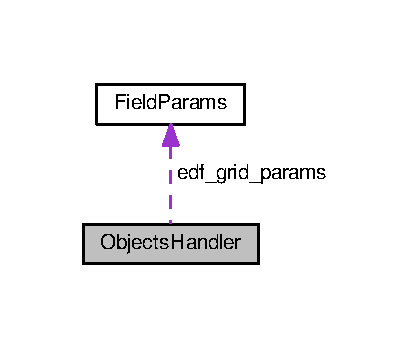
\includegraphics[width=198pt]{class_objects_handler__coll__graph}
\end{center}
\end{figure}
\subsection*{Public Member Functions}
\begin{DoxyCompactItemize}
\item 
\hyperlink{class_objects_handler_a932c6bc722daa78f4f8e31894911c4c7}{Objects\+Handler} ()
\item 
void \hyperlink{class_objects_handler_a1ac7fcad5fa6033c2435ac49f2f9dff5}{init} (ros\+::\+Node\+Handle nh)
\item 
void \hyperlink{class_objects_handler_ae6da4f0f0a265c75722e02d68d519f07}{compute\+\_\+edf} ()
\item 
\hyperlink{class_objects_handler_a5d3298d7029619c1931d3dda34278e05}{Objects\+Handler} (ros\+::\+Node\+Handle nh)
\item 
Pose\+Stamped \hyperlink{class_objects_handler_a2b9e69afe54afea0380431d8f1f5142d}{get\+\_\+target\+\_\+pose} ()
\item 
Pose\+Stamped \hyperlink{class_objects_handler_a4ac7a7bb712575c2ff6ffbf37144cf56}{get\+\_\+chaser\+\_\+pose} ()
\item 
Twist \hyperlink{class_objects_handler_aa1af309b0e964ccb6df8dede045fa32b}{get\+\_\+chaser\+\_\+velocity} ()
\item 
Twist \hyperlink{class_objects_handler_a41d48832b07a4d4276147a99dd1d31bc}{get\+\_\+chaser\+\_\+acceleration} ()
\item 
string \hyperlink{class_objects_handler_a07e9d105db04be181661dc979314de3c}{get\+\_\+world\+\_\+frame\+\_\+id} ()
\item 
octomap\+::\+Oc\+Tree $\ast$ \hyperlink{class_objects_handler_a988bdf05045c40348b34ae8beecd8884}{get\+\_\+octree\+\_\+obj\+\_\+ptr} ()
\item 
\hyperlink{struct_grid_field}{Grid\+Field} $\ast$ \hyperlink{class_objects_handler_afe849882d1feeef8316a45632381da54}{get\+\_\+edf\+\_\+grid\+\_\+ptr} ()
\item 
void \hyperlink{class_objects_handler_a5744110d979850b3e2d8896793435d0c}{octomap\+\_\+callback} (const octomap\+\_\+msgs\+::\+Octomap \&msg)
\item 
void \hyperlink{class_objects_handler_a968feba95e0707919b6c3632781510ba}{chaser\+\_\+spawn} (Pose\+Stamped spawn\+\_\+pose)
\item 
void \hyperlink{class_objects_handler_a4c56416d3583b70d181d69d900b884b5}{callback\+\_\+chaser\+\_\+init\+\_\+pose} (const geometry\+\_\+msgs\+::\+Pose\+Stamped\+Const\+Ptr \&chaser\+\_\+init\+\_\+pose)
\item 
void \hyperlink{class_objects_handler_a28ac9c7ef998a413825cddca78324f61}{callback\+\_\+chaser\+\_\+control\+\_\+pose} (const geometry\+\_\+msgs\+::\+Pose\+Stamped\+Const\+Ptr \&chaser\+\_\+control\+\_\+pose)
\begin{DoxyCompactList}\small\item\em callback function for control pose from wrapper. This is intended to replace the currnet chaser pose directly with desired pose \end{DoxyCompactList}\item 
void \hyperlink{class_objects_handler_a6896e4f9863bd1a4fbc8498d0cb20f09}{tf\+\_\+update} ()
\item 
void \hyperlink{class_objects_handler_a16cf7fca3059a03da4ec795f2af7fb74}{publish} ()
\item 
vector$<$ Point $>$ \hyperlink{class_objects_handler_a4793f1ed257c849b28f0386f635ee714}{get\+\_\+prediction\+\_\+seq} ()
\end{DoxyCompactItemize}
\subsection*{Public Attributes}
\begin{DoxyCompactItemize}
\item 
bool \hyperlink{class_objects_handler_a56f70ac04c01e8b948a4b44fa5670f49}{is\+\_\+octomap\+\_\+full} = false
\item 
bool \hyperlink{class_objects_handler_a86f8528ff5697c87fc6a3fcd6ba0f42c}{is\+\_\+chaser\+\_\+recieved} = false
\item 
bool \hyperlink{class_objects_handler_acf1ef1b318defc2a39d87cea72689478}{is\+\_\+map\+\_\+recieved} = false
\item 
bool \hyperlink{class_objects_handler_a7691f3e1ec58e55ead30c50c555f169a}{is\+\_\+target\+\_\+recieved} = false
\item 
bool \hyperlink{class_objects_handler_a88fb913340c535df81f3b7ae5f06df61}{is\+\_\+control\+\_\+received} = false
\item 
bool \hyperlink{class_objects_handler_a16165ae7c0167ba8d2a0151a8a4fbfd5}{is\+\_\+chaser\+\_\+spawned} = false
\item 
bool \hyperlink{class_objects_handler_acaefe98eb412d4c32cda2bf0bd602ae7}{is\+\_\+insert\+\_\+permit} = false
\item 
bool \hyperlink{class_objects_handler_ad8d1ea6646024f0a03e154a7c2c07682}{is\+\_\+path\+\_\+solved} = false
\end{DoxyCompactItemize}
\subsection*{Private Attributes}
\begin{DoxyCompactItemize}
\item 
ros\+::\+Subscriber \hyperlink{class_objects_handler_a3b384ae3f8f66557b1c1ac04523fb330}{sub\+\_\+octomap}
\item 
ros\+::\+Subscriber \hyperlink{class_objects_handler_a9a2e098b85260b71c88b81dadd6ca58a}{sub\+\_\+chaser\+\_\+init\+\_\+pose}
\item 
ros\+::\+Subscriber \hyperlink{class_objects_handler_adc3a2895e97bb2349fb5cb71d4eec191}{sub\+\_\+chaser\+\_\+control\+\_\+pose}
\item 
ros\+::\+Publisher \hyperlink{class_objects_handler_a86a1f98983b533f77bf17867affb5251}{pub\+\_\+edf}
\item 
visualization\+\_\+msgs\+::\+Marker \hyperlink{class_objects_handler_ad6904dcaaad790234569760df0fb0ac2}{markers\+\_\+edf}
\item 
tf\+::\+Transform\+Listener $\ast$ \hyperlink{class_objects_handler_aea45bba31aa769008386100725bda66b}{tf\+\_\+listener}
\item 
tf\+::\+Transform\+Broadcaster $\ast$ \hyperlink{class_objects_handler_af49de4eabb124e2ee6c9e12ebb31bca3}{tf\+\_\+talker}
\item 
string \hyperlink{class_objects_handler_a1c0586ae7467bb8a3df8ad247ac7b10b}{world\+\_\+frame\+\_\+id}
\item 
string \hyperlink{class_objects_handler_a3e8d08bf5d76d69f1768b53fd799953c}{chaser\+\_\+frame\+\_\+id}
\item 
string \hyperlink{class_objects_handler_a7a616768386c4c7da9af4da3d07bd936}{target\+\_\+frame\+\_\+id}
\item 
string \hyperlink{class_objects_handler_a70b5e252a180d919653c7b53aff6f534}{octomap\+\_\+topic\+\_\+name}
\item 
Pose\+Stamped \hyperlink{class_objects_handler_ad436bfd8b262f473f0e4ca92b3c3402b}{target\+\_\+pose}
\item 
Pose\+Stamped \hyperlink{class_objects_handler_a79fd5f872a40cca5ea599f1e83dcb3ad}{chaser\+\_\+pose}
\item 
Twist \hyperlink{class_objects_handler_a74e3f3b4bf263711c389190a595368e2}{chaser\+\_\+vel}
\item 
Twist \hyperlink{class_objects_handler_a36db60068ada56b9142b3d6ef0437749}{chaser\+\_\+acc}
\item 
shared\+\_\+ptr$<$ octomap\+::\+Oc\+Tree $>$ \hyperlink{class_objects_handler_a76ad7ca7513755408c02dd36dea94c6e}{octree\+\_\+ptr}
\item 
Dynamic\+E\+D\+T\+Octomap $\ast$ \hyperlink{class_objects_handler_aa96d8c71f5e8c6423c88d3302220d4cf}{edf\+\_\+ptr}
\item 
shared\+\_\+ptr$<$ \hyperlink{struct_grid_field}{Grid\+Field} $>$ \hyperlink{class_objects_handler_af2063609510d5ad8f136a275b0d127c1}{edf\+\_\+grid\+\_\+ptr}
\item 
double \hyperlink{class_objects_handler_ac8c10c7a10aeb8abf1a44b7361f646e6}{min\+\_\+z}
\item 
double \hyperlink{class_objects_handler_aa991434e17ca1144c80633ff7530534c}{chaser\+\_\+init\+\_\+z}
\item 
double \hyperlink{class_objects_handler_a577e8b62f1e55d36330048fb9fd3a432}{edf\+\_\+max\+\_\+viz\+\_\+dist}
\item 
double \hyperlink{class_objects_handler_ae71885df3c4e28f45be7bb0e5a383293}{edf\+\_\+max\+\_\+dist}
\item 
\hyperlink{struct_field_params}{Field\+Params} \hyperlink{class_objects_handler_a46ed8cfd250b183909a7d3a1f56cee6b}{edf\+\_\+grid\+\_\+params}
\item 
int \hyperlink{class_objects_handler_a95908d5b00f62b629dc7f20acb714292}{run\+\_\+mode}
\end{DoxyCompactItemize}


\subsection{Detailed Description}


\subsection{Constructor \& Destructor Documentation}
\index{Objects\+Handler@{Objects\+Handler}!Objects\+Handler@{Objects\+Handler}}
\index{Objects\+Handler@{Objects\+Handler}!Objects\+Handler@{Objects\+Handler}}
\subsubsection[{\texorpdfstring{Objects\+Handler()}{ObjectsHandler()}}]{\setlength{\rightskip}{0pt plus 5cm}Objects\+Handler\+::\+Objects\+Handler (
\begin{DoxyParamCaption}
{}
\end{DoxyParamCaption}
)\hspace{0.3cm}{\ttfamily [inline]}}\hypertarget{class_objects_handler_a932c6bc722daa78f4f8e31894911c4c7}{}\label{class_objects_handler_a932c6bc722daa78f4f8e31894911c4c7}

\begin{DoxyCode}
56 \{\};
\end{DoxyCode}
\index{Objects\+Handler@{Objects\+Handler}!Objects\+Handler@{Objects\+Handler}}
\index{Objects\+Handler@{Objects\+Handler}!Objects\+Handler@{Objects\+Handler}}
\subsubsection[{\texorpdfstring{Objects\+Handler(ros\+::\+Node\+Handle nh)}{ObjectsHandler(ros::NodeHandle nh)}}]{\setlength{\rightskip}{0pt plus 5cm}Objects\+Handler\+::\+Objects\+Handler (
\begin{DoxyParamCaption}
\item[{ros\+::\+Node\+Handle}]{nh}
\end{DoxyParamCaption}
)}\hypertarget{class_objects_handler_a5d3298d7029619c1931d3dda34278e05}{}\label{class_objects_handler_a5d3298d7029619c1931d3dda34278e05}

\begin{DoxyCode}
3 \{\};
\end{DoxyCode}


\subsection{Member Function Documentation}
\index{Objects\+Handler@{Objects\+Handler}!callback\+\_\+chaser\+\_\+control\+\_\+pose@{callback\+\_\+chaser\+\_\+control\+\_\+pose}}
\index{callback\+\_\+chaser\+\_\+control\+\_\+pose@{callback\+\_\+chaser\+\_\+control\+\_\+pose}!Objects\+Handler@{Objects\+Handler}}
\subsubsection[{\texorpdfstring{callback\+\_\+chaser\+\_\+control\+\_\+pose(const geometry\+\_\+msgs\+::\+Pose\+Stamped\+Const\+Ptr \&chaser\+\_\+control\+\_\+pose)}{callback_chaser_control_pose(const geometry_msgs::PoseStampedConstPtr &chaser_control_pose)}}]{\setlength{\rightskip}{0pt plus 5cm}void Objects\+Handler\+::callback\+\_\+chaser\+\_\+control\+\_\+pose (
\begin{DoxyParamCaption}
\item[{const geometry\+\_\+msgs\+::\+Pose\+Stamped\+Const\+Ptr \&}]{chaser\+\_\+control\+\_\+pose}
\end{DoxyParamCaption}
)}\hypertarget{class_objects_handler_a28ac9c7ef998a413825cddca78324f61}{}\label{class_objects_handler_a28ac9c7ef998a413825cddca78324f61}


callback function for control pose from wrapper. This is intended to replace the currnet chaser pose directly with desired pose 


\begin{DoxyParams}{Parameters}
{\em chaser\+\_\+control\+\_\+pose} & \\
\hline
\end{DoxyParams}

\begin{DoxyCode}
278                                                                                                            
       \{
279     \textcolor{keywordflow}{if}(\hyperlink{class_objects_handler_a95908d5b00f62b629dc7f20acb714292}{run\_mode} == 0 and \hyperlink{class_objects_handler_ad8d1ea6646024f0a03e154a7c2c07682}{is\_path\_solved})\{
280         \hyperlink{class_objects_handler_a79fd5f872a40cca5ea599f1e83dcb3ad}{chaser\_pose} = *chaser\_control\_pose;
281     \}
282     
283 \}
\end{DoxyCode}
\index{Objects\+Handler@{Objects\+Handler}!callback\+\_\+chaser\+\_\+init\+\_\+pose@{callback\+\_\+chaser\+\_\+init\+\_\+pose}}
\index{callback\+\_\+chaser\+\_\+init\+\_\+pose@{callback\+\_\+chaser\+\_\+init\+\_\+pose}!Objects\+Handler@{Objects\+Handler}}
\subsubsection[{\texorpdfstring{callback\+\_\+chaser\+\_\+init\+\_\+pose(const geometry\+\_\+msgs\+::\+Pose\+Stamped\+Const\+Ptr \&chaser\+\_\+init\+\_\+pose)}{callback_chaser_init_pose(const geometry_msgs::PoseStampedConstPtr &chaser_init_pose)}}]{\setlength{\rightskip}{0pt plus 5cm}void Objects\+Handler\+::callback\+\_\+chaser\+\_\+init\+\_\+pose (
\begin{DoxyParamCaption}
\item[{const geometry\+\_\+msgs\+::\+Pose\+Stamped\+Const\+Ptr \&}]{chaser\+\_\+init\+\_\+pose}
\end{DoxyParamCaption}
)}\hypertarget{class_objects_handler_a4c56416d3583b70d181d69d900b884b5}{}\label{class_objects_handler_a4c56416d3583b70d181d69d900b884b5}

\begin{DoxyCode}
269                                                                                                       \{
270 
271     \hyperlink{class_objects_handler_a968feba95e0707919b6c3632781510ba}{chaser\_spawn}(*chaser\_init\_pose);    
272 \}
\end{DoxyCode}
\index{Objects\+Handler@{Objects\+Handler}!chaser\+\_\+spawn@{chaser\+\_\+spawn}}
\index{chaser\+\_\+spawn@{chaser\+\_\+spawn}!Objects\+Handler@{Objects\+Handler}}
\subsubsection[{\texorpdfstring{chaser\+\_\+spawn(\+Pose\+Stamped spawn\+\_\+pose)}{chaser_spawn(PoseStamped spawn_pose)}}]{\setlength{\rightskip}{0pt plus 5cm}void Objects\+Handler\+::chaser\+\_\+spawn (
\begin{DoxyParamCaption}
\item[{Pose\+Stamped}]{spawn\+\_\+pose}
\end{DoxyParamCaption}
)}\hypertarget{class_objects_handler_a968feba95e0707919b6c3632781510ba}{}\label{class_objects_handler_a968feba95e0707919b6c3632781510ba}

\begin{DoxyCode}
253                                                        \{
254     ROS\_INFO\_ONCE(\textcolor{stringliteral}{"[Objects handler] spawning chaser."}); 
255     
256     \hyperlink{class_objects_handler_a86f8528ff5697c87fc6a3fcd6ba0f42c}{is\_chaser\_recieved} = \textcolor{keyword}{true};
257     \hyperlink{class_objects_handler_a16165ae7c0167ba8d2a0151a8a4fbfd5}{is\_chaser\_spawned} = \textcolor{keyword}{true};    
258     
259     \textcolor{keywordflow}{if}(\hyperlink{class_objects_handler_a95908d5b00f62b629dc7f20acb714292}{run\_mode} == 0)\{ \textcolor{comment}{// without gazebo : update chaser pose}
260         \hyperlink{class_objects_handler_a79fd5f872a40cca5ea599f1e83dcb3ad}{chaser\_pose} = spawn\_pose;
261         \hyperlink{class_objects_handler_a79fd5f872a40cca5ea599f1e83dcb3ad}{chaser\_pose}.pose.position.z = \hyperlink{class_objects_handler_aa991434e17ca1144c80633ff7530534c}{chaser\_init\_z};
262 
263     \}\textcolor{keywordflow}{else}\{ \textcolor{comment}{// with gazebo : nothing happen }
264         ROS\_WARN(\textcolor{stringliteral}{"[Object Handler] gazebo mode. No virtual spawning happens"});        
265     \}
266 
267 \}
\end{DoxyCode}
\index{Objects\+Handler@{Objects\+Handler}!compute\+\_\+edf@{compute\+\_\+edf}}
\index{compute\+\_\+edf@{compute\+\_\+edf}!Objects\+Handler@{Objects\+Handler}}
\subsubsection[{\texorpdfstring{compute\+\_\+edf()}{compute_edf()}}]{\setlength{\rightskip}{0pt plus 5cm}void Objects\+Handler\+::compute\+\_\+edf (
\begin{DoxyParamCaption}
{}
\end{DoxyParamCaption}
)}\hypertarget{class_objects_handler_ae6da4f0f0a265c75722e02d68d519f07}{}\label{class_objects_handler_ae6da4f0f0a265c75722e02d68d519f07}

\begin{DoxyCode}
222                                 \{
223 
224     \textcolor{keywordflow}{for}(\textcolor{keywordtype}{int} ix = 0 ; ix<\hyperlink{class_objects_handler_af2063609510d5ad8f136a275b0d127c1}{edf\_grid\_ptr}.get()->Nx ; ix++)
225         \textcolor{keywordflow}{for}(\textcolor{keywordtype}{int} iy = 0 ; iy<\hyperlink{class_objects_handler_af2063609510d5ad8f136a275b0d127c1}{edf\_grid\_ptr}.get()->Ny ; iy++)
226             \textcolor{keywordflow}{for}(\textcolor{keywordtype}{int} iz = 0 ; iz<\hyperlink{class_objects_handler_af2063609510d5ad8f136a275b0d127c1}{edf\_grid\_ptr}.get()->Nz ; iz++)\{
227                 Point eval\_pnt = \hyperlink{class_objects_handler_af2063609510d5ad8f136a275b0d127c1}{edf\_grid\_ptr}.get()->getCellPnt(Vector3i(ix,iy,iz));  
228                 \textcolor{comment}{// query edf value from edf mapper                       }
229                 \textcolor{keywordtype}{float} dist\_val = \hyperlink{class_objects_handler_aa96d8c71f5e8c6423c88d3302220d4cf}{edf\_ptr}->getDistance(octomap::point3d(eval\_pnt.x,eval\_pnt.y,
      eval\_pnt.z));
230 
231                 \textcolor{comment}{// edf value assign to homogenous grid  }
232                 \hyperlink{class_objects_handler_af2063609510d5ad8f136a275b0d127c1}{edf\_grid\_ptr}.get()->field\_vals[ix][iy][iz] = dist\_val;
233 
234                 \textcolor{comment}{// marker generation}
235                 \textcolor{keywordflow}{if}(dist\_val<\hyperlink{class_objects_handler_a577e8b62f1e55d36330048fb9fd3a432}{edf\_max\_viz\_dist})\{                
236                     \textcolor{comment}{// color }
237                     std\_msgs::ColorRGBA color;                    
238                     \hyperlink{_common_8h_a4b2e4b6698ff92678b23392dc111b36d}{get\_color\_dist}(dist\_val,color,\hyperlink{class_objects_handler_a577e8b62f1e55d36330048fb9fd3a432}{edf\_max\_viz\_dist});
239 
240                     \textcolor{comment}{// marker }
241                     \hyperlink{class_objects_handler_ad6904dcaaad790234569760df0fb0ac2}{markers\_edf}.points.push\_back(eval\_pnt);
242                     \hyperlink{class_objects_handler_ad6904dcaaad790234569760df0fb0ac2}{markers\_edf}.colors.push\_back(color);                    
243                 \}
244             \}    
245 
246 \}
\end{DoxyCode}
\index{Objects\+Handler@{Objects\+Handler}!get\+\_\+chaser\+\_\+acceleration@{get\+\_\+chaser\+\_\+acceleration}}
\index{get\+\_\+chaser\+\_\+acceleration@{get\+\_\+chaser\+\_\+acceleration}!Objects\+Handler@{Objects\+Handler}}
\subsubsection[{\texorpdfstring{get\+\_\+chaser\+\_\+acceleration()}{get_chaser_acceleration()}}]{\setlength{\rightskip}{0pt plus 5cm}Twist Objects\+Handler\+::get\+\_\+chaser\+\_\+acceleration (
\begin{DoxyParamCaption}
{}
\end{DoxyParamCaption}
)}\hypertarget{class_objects_handler_a41d48832b07a4d4276147a99dd1d31bc}{}\label{class_objects_handler_a41d48832b07a4d4276147a99dd1d31bc}

\begin{DoxyCode}
120 \{\textcolor{keywordflow}{return} \hyperlink{class_objects_handler_a36db60068ada56b9142b3d6ef0437749}{chaser\_acc};\};
\end{DoxyCode}
\index{Objects\+Handler@{Objects\+Handler}!get\+\_\+chaser\+\_\+pose@{get\+\_\+chaser\+\_\+pose}}
\index{get\+\_\+chaser\+\_\+pose@{get\+\_\+chaser\+\_\+pose}!Objects\+Handler@{Objects\+Handler}}
\subsubsection[{\texorpdfstring{get\+\_\+chaser\+\_\+pose()}{get_chaser_pose()}}]{\setlength{\rightskip}{0pt plus 5cm}Pose\+Stamped Objects\+Handler\+::get\+\_\+chaser\+\_\+pose (
\begin{DoxyParamCaption}
{}
\end{DoxyParamCaption}
)}\hypertarget{class_objects_handler_a4ac7a7bb712575c2ff6ffbf37144cf56}{}\label{class_objects_handler_a4ac7a7bb712575c2ff6ffbf37144cf56}

\begin{DoxyCode}
118 \{\textcolor{keywordflow}{return} \hyperlink{class_objects_handler_a79fd5f872a40cca5ea599f1e83dcb3ad}{chaser\_pose};\};
\end{DoxyCode}
\index{Objects\+Handler@{Objects\+Handler}!get\+\_\+chaser\+\_\+velocity@{get\+\_\+chaser\+\_\+velocity}}
\index{get\+\_\+chaser\+\_\+velocity@{get\+\_\+chaser\+\_\+velocity}!Objects\+Handler@{Objects\+Handler}}
\subsubsection[{\texorpdfstring{get\+\_\+chaser\+\_\+velocity()}{get_chaser_velocity()}}]{\setlength{\rightskip}{0pt plus 5cm}Twist Objects\+Handler\+::get\+\_\+chaser\+\_\+velocity (
\begin{DoxyParamCaption}
{}
\end{DoxyParamCaption}
)}\hypertarget{class_objects_handler_aa1af309b0e964ccb6df8dede045fa32b}{}\label{class_objects_handler_aa1af309b0e964ccb6df8dede045fa32b}

\begin{DoxyCode}
119 \{\textcolor{keywordflow}{return} \hyperlink{class_objects_handler_a74e3f3b4bf263711c389190a595368e2}{chaser\_vel};\};
\end{DoxyCode}
\index{Objects\+Handler@{Objects\+Handler}!get\+\_\+edf\+\_\+grid\+\_\+ptr@{get\+\_\+edf\+\_\+grid\+\_\+ptr}}
\index{get\+\_\+edf\+\_\+grid\+\_\+ptr@{get\+\_\+edf\+\_\+grid\+\_\+ptr}!Objects\+Handler@{Objects\+Handler}}
\subsubsection[{\texorpdfstring{get\+\_\+edf\+\_\+grid\+\_\+ptr()}{get_edf_grid_ptr()}}]{\setlength{\rightskip}{0pt plus 5cm}{\bf Grid\+Field} $\ast$ Objects\+Handler\+::get\+\_\+edf\+\_\+grid\+\_\+ptr (
\begin{DoxyParamCaption}
{}
\end{DoxyParamCaption}
)}\hypertarget{class_objects_handler_afe849882d1feeef8316a45632381da54}{}\label{class_objects_handler_afe849882d1feeef8316a45632381da54}

\begin{DoxyCode}
123 \{\textcolor{keywordflow}{return} \hyperlink{class_objects_handler_af2063609510d5ad8f136a275b0d127c1}{edf\_grid\_ptr}.get();\};
\end{DoxyCode}
\index{Objects\+Handler@{Objects\+Handler}!get\+\_\+octree\+\_\+obj\+\_\+ptr@{get\+\_\+octree\+\_\+obj\+\_\+ptr}}
\index{get\+\_\+octree\+\_\+obj\+\_\+ptr@{get\+\_\+octree\+\_\+obj\+\_\+ptr}!Objects\+Handler@{Objects\+Handler}}
\subsubsection[{\texorpdfstring{get\+\_\+octree\+\_\+obj\+\_\+ptr()}{get_octree_obj_ptr()}}]{\setlength{\rightskip}{0pt plus 5cm}octomap\+::\+Oc\+Tree $\ast$ Objects\+Handler\+::get\+\_\+octree\+\_\+obj\+\_\+ptr (
\begin{DoxyParamCaption}
{}
\end{DoxyParamCaption}
)}\hypertarget{class_objects_handler_a988bdf05045c40348b34ae8beecd8884}{}\label{class_objects_handler_a988bdf05045c40348b34ae8beecd8884}

\begin{DoxyCode}
122 \{\textcolor{keywordflow}{return} \hyperlink{class_objects_handler_a76ad7ca7513755408c02dd36dea94c6e}{octree\_ptr}.get();\};
\end{DoxyCode}
\index{Objects\+Handler@{Objects\+Handler}!get\+\_\+prediction\+\_\+seq@{get\+\_\+prediction\+\_\+seq}}
\index{get\+\_\+prediction\+\_\+seq@{get\+\_\+prediction\+\_\+seq}!Objects\+Handler@{Objects\+Handler}}
\subsubsection[{\texorpdfstring{get\+\_\+prediction\+\_\+seq()}{get_prediction_seq()}}]{\setlength{\rightskip}{0pt plus 5cm}vector$<$ Point $>$ Objects\+Handler\+::get\+\_\+prediction\+\_\+seq (
\begin{DoxyParamCaption}
{}
\end{DoxyParamCaption}
)}\hypertarget{class_objects_handler_a4793f1ed257c849b28f0386f635ee714}{}\label{class_objects_handler_a4793f1ed257c849b28f0386f635ee714}

\begin{DoxyCode}
286                                                 \{
287     
288     
289 \}
\end{DoxyCode}
\index{Objects\+Handler@{Objects\+Handler}!get\+\_\+target\+\_\+pose@{get\+\_\+target\+\_\+pose}}
\index{get\+\_\+target\+\_\+pose@{get\+\_\+target\+\_\+pose}!Objects\+Handler@{Objects\+Handler}}
\subsubsection[{\texorpdfstring{get\+\_\+target\+\_\+pose()}{get_target_pose()}}]{\setlength{\rightskip}{0pt plus 5cm}Pose\+Stamped Objects\+Handler\+::get\+\_\+target\+\_\+pose (
\begin{DoxyParamCaption}
{}
\end{DoxyParamCaption}
)}\hypertarget{class_objects_handler_a2b9e69afe54afea0380431d8f1f5142d}{}\label{class_objects_handler_a2b9e69afe54afea0380431d8f1f5142d}

\begin{DoxyCode}
111                                             \{
112     PoseStamped pose(\hyperlink{class_objects_handler_ad436bfd8b262f473f0e4ca92b3c3402b}{target\_pose}); 
113     pose.pose.position.z = \hyperlink{class_objects_handler_ac8c10c7a10aeb8abf1a44b7361f646e6}{min\_z}; 
114     \textcolor{keywordflow}{return} pose;
115 \};
\end{DoxyCode}
\index{Objects\+Handler@{Objects\+Handler}!get\+\_\+world\+\_\+frame\+\_\+id@{get\+\_\+world\+\_\+frame\+\_\+id}}
\index{get\+\_\+world\+\_\+frame\+\_\+id@{get\+\_\+world\+\_\+frame\+\_\+id}!Objects\+Handler@{Objects\+Handler}}
\subsubsection[{\texorpdfstring{get\+\_\+world\+\_\+frame\+\_\+id()}{get_world_frame_id()}}]{\setlength{\rightskip}{0pt plus 5cm}string Objects\+Handler\+::get\+\_\+world\+\_\+frame\+\_\+id (
\begin{DoxyParamCaption}
{}
\end{DoxyParamCaption}
)}\hypertarget{class_objects_handler_a07e9d105db04be181661dc979314de3c}{}\label{class_objects_handler_a07e9d105db04be181661dc979314de3c}

\begin{DoxyCode}
121 \{\textcolor{keywordflow}{return} \hyperlink{class_objects_handler_a1c0586ae7467bb8a3df8ad247ac7b10b}{world\_frame\_id};\};
\end{DoxyCode}
\index{Objects\+Handler@{Objects\+Handler}!init@{init}}
\index{init@{init}!Objects\+Handler@{Objects\+Handler}}
\subsubsection[{\texorpdfstring{init(ros\+::\+Node\+Handle nh)}{init(ros::NodeHandle nh)}}]{\setlength{\rightskip}{0pt plus 5cm}void Objects\+Handler\+::init (
\begin{DoxyParamCaption}
\item[{ros\+::\+Node\+Handle}]{nh}
\end{DoxyParamCaption}
)}\hypertarget{class_objects_handler_a1ac7fcad5fa6033c2435ac49f2f9dff5}{}\label{class_objects_handler_a1ac7fcad5fa6033c2435ac49f2f9dff5}

\begin{DoxyCode}
5                                          \{
6 
7     \textcolor{comment}{// parameters}
8     nh.param<\textcolor{keywordtype}{string}>(\textcolor{stringliteral}{"world\_frame\_id"},this->\hyperlink{class_objects_handler_a1c0586ae7467bb8a3df8ad247ac7b10b}{world\_frame\_id},\textcolor{stringliteral}{"/world"});
9     nh.param<\textcolor{keywordtype}{string}>(\textcolor{stringliteral}{"target\_frame\_id"},this->\hyperlink{class_objects_handler_a7a616768386c4c7da9af4da3d07bd936}{target\_frame\_id},\textcolor{stringliteral}{"/target\_\_base\_footprint"});
10     nh.param<\textcolor{keywordtype}{string}>(\textcolor{stringliteral}{"chaser\_frame\_id"},this->\hyperlink{class_objects_handler_a3e8d08bf5d76d69f1768b53fd799953c}{chaser\_frame\_id},\textcolor{stringliteral}{"/firefly/base\_link"}); 
11 
12     \textcolor{comment}{// for chaser spawning }
13      
14     \textcolor{comment}{// edf grid param}
15     nh.param(\textcolor{stringliteral}{"min\_z"},\hyperlink{class_objects_handler_ac8c10c7a10aeb8abf1a44b7361f646e6}{min\_z},0.4);   
16     nh.param(\textcolor{stringliteral}{"chaser\_init\_z"},\hyperlink{class_objects_handler_aa991434e17ca1144c80633ff7530534c}{chaser\_init\_z},1.0);             
17     nh.param(\textcolor{stringliteral}{"edf\_max\_dist"},\hyperlink{class_objects_handler_ae71885df3c4e28f45be7bb0e5a383293}{edf\_max\_dist},2.0);  
18     nh.param(\textcolor{stringliteral}{"edf\_max\_plot\_dist"},\hyperlink{class_objects_handler_a577e8b62f1e55d36330048fb9fd3a432}{edf\_max\_viz\_dist},0.5);  
19     nh.param(\textcolor{stringliteral}{"edf\_resolution"},\hyperlink{class_objects_handler_a46ed8cfd250b183909a7d3a1f56cee6b}{edf\_grid\_params}.\hyperlink{struct_field_params_a520406c76b3abf392401626bc2161370}{resolution},0.5);  
20     nh.param(\textcolor{stringliteral}{"edf\_stride\_resolution"},\hyperlink{class_objects_handler_a46ed8cfd250b183909a7d3a1f56cee6b}{edf\_grid\_params}.
      \hyperlink{struct_field_params_ae6eabaa6e593c9dbac48b2f96bea80ec}{ray\_stride\_res},0.3);  
21     nh.param(\textcolor{stringliteral}{"run\_mode"},\hyperlink{class_objects_handler_a95908d5b00f62b629dc7f20acb714292}{run\_mode},0);  
22 
23 
24     \hyperlink{class_objects_handler_ad436bfd8b262f473f0e4ca92b3c3402b}{target\_pose}.header.frame\_id = \hyperlink{class_objects_handler_a1c0586ae7467bb8a3df8ad247ac7b10b}{world\_frame\_id};
25     \hyperlink{class_objects_handler_a79fd5f872a40cca5ea599f1e83dcb3ad}{chaser\_pose}.header.frame\_id = \hyperlink{class_objects_handler_a1c0586ae7467bb8a3df8ad247ac7b10b}{world\_frame\_id};
26     \hyperlink{class_objects_handler_ad6904dcaaad790234569760df0fb0ac2}{markers\_edf}.header.frame\_id = \hyperlink{class_objects_handler_a1c0586ae7467bb8a3df8ad247ac7b10b}{world\_frame\_id};
27 
28     \hyperlink{class_objects_handler_ad6904dcaaad790234569760df0fb0ac2}{markers\_edf}.action = visualization\_msgs::Marker::ADD;
29     \hyperlink{class_objects_handler_ad6904dcaaad790234569760df0fb0ac2}{markers\_edf}.type = visualization\_msgs::Marker::CUBE\_LIST;      
30     \hyperlink{class_objects_handler_ad6904dcaaad790234569760df0fb0ac2}{markers\_edf}.pose.orientation.x = 0;
31     \hyperlink{class_objects_handler_ad6904dcaaad790234569760df0fb0ac2}{markers\_edf}.pose.orientation.y = 0;
32     \hyperlink{class_objects_handler_ad6904dcaaad790234569760df0fb0ac2}{markers\_edf}.pose.orientation.z = 0;
33     \hyperlink{class_objects_handler_ad6904dcaaad790234569760df0fb0ac2}{markers\_edf}.pose.orientation.w = 1;                  
34     \hyperlink{class_objects_handler_ad6904dcaaad790234569760df0fb0ac2}{markers\_edf}.scale.x = \hyperlink{class_objects_handler_a46ed8cfd250b183909a7d3a1f56cee6b}{edf\_grid\_params}.\hyperlink{struct_field_params_a520406c76b3abf392401626bc2161370}{resolution};
35     \hyperlink{class_objects_handler_ad6904dcaaad790234569760df0fb0ac2}{markers\_edf}.scale.y = \hyperlink{class_objects_handler_a46ed8cfd250b183909a7d3a1f56cee6b}{edf\_grid\_params}.\hyperlink{struct_field_params_a520406c76b3abf392401626bc2161370}{resolution};
36     \hyperlink{class_objects_handler_ad6904dcaaad790234569760df0fb0ac2}{markers\_edf}.scale.z = \hyperlink{class_objects_handler_a46ed8cfd250b183909a7d3a1f56cee6b}{edf\_grid\_params}.\hyperlink{struct_field_params_a520406c76b3abf392401626bc2161370}{resolution};
37     
38     
39     \textcolor{comment}{// topics }
40     \hyperlink{class_objects_handler_aea45bba31aa769008386100725bda66b}{tf\_listener} = \textcolor{keyword}{new} (tf::TransformListener);
41     \hyperlink{class_objects_handler_af49de4eabb124e2ee6c9e12ebb31bca3}{tf\_talker} = \textcolor{keyword}{new} (tf::TransformBroadcaster);
42 
43     \hyperlink{class_objects_handler_a86a1f98983b533f77bf17867affb5251}{pub\_edf} = nh.advertise<visualization\_msgs::Marker>(\textcolor{stringliteral}{"edf\_grid"},1);
44 
45     \textcolor{comment}{// octomap            }
46     nh.param(\textcolor{stringliteral}{"is\_octomap\_full"},this->\hyperlink{class_objects_handler_a56f70ac04c01e8b948a4b44fa5670f49}{is\_octomap\_full},\textcolor{keyword}{true});
47     \hyperlink{class_objects_handler_a76ad7ca7513755408c02dd36dea94c6e}{octree\_ptr}.reset(\textcolor{keyword}{new} octomap::OcTree(0.1)); \textcolor{comment}{// arbitrary init}
48     \textcolor{keywordflow}{if} (\hyperlink{class_objects_handler_a56f70ac04c01e8b948a4b44fa5670f49}{is\_octomap\_full})
49         \hyperlink{class_objects_handler_a3b384ae3f8f66557b1c1ac04523fb330}{sub\_octomap} = nh.subscribe(\textcolor{stringliteral}{"/octomap\_full"},1,&
      \hyperlink{class_objects_handler_a5744110d979850b3e2d8896793435d0c}{ObjectsHandler::octomap\_callback},\textcolor{keyword}{this});   
50     \textcolor{keywordflow}{else}
51         \hyperlink{class_objects_handler_a3b384ae3f8f66557b1c1ac04523fb330}{sub\_octomap} = nh.subscribe(\textcolor{stringliteral}{"/octomap\_binary"},1,&
      \hyperlink{class_objects_handler_a5744110d979850b3e2d8896793435d0c}{ObjectsHandler::octomap\_callback},\textcolor{keyword}{this});   
52 
53     \hyperlink{class_objects_handler_a9a2e098b85260b71c88b81dadd6ca58a}{sub\_chaser\_init\_pose} = nh.subscribe(\textcolor{stringliteral}{"/chaser\_init\_pose"},1,&
      \hyperlink{class_objects_handler_a4c56416d3583b70d181d69d900b884b5}{ObjectsHandler::callback\_chaser\_init\_pose},\textcolor{keyword}{this});
54     \hyperlink{class_objects_handler_adc3a2895e97bb2349fb5cb71d4eec191}{sub\_chaser\_control\_pose} = nh.subscribe(\textcolor{stringliteral}{"mav\_pose\_desired"},1,&
      \hyperlink{class_objects_handler_a28ac9c7ef998a413825cddca78324f61}{ObjectsHandler::callback\_chaser\_control\_pose},\textcolor{keyword}{this});
55     
56     ROS\_INFO(\textcolor{stringliteral}{"Object handler initialized."}); 
57 \}
\end{DoxyCode}
\index{Objects\+Handler@{Objects\+Handler}!octomap\+\_\+callback@{octomap\+\_\+callback}}
\index{octomap\+\_\+callback@{octomap\+\_\+callback}!Objects\+Handler@{Objects\+Handler}}
\subsubsection[{\texorpdfstring{octomap\+\_\+callback(const octomap\+\_\+msgs\+::\+Octomap \&msg)}{octomap_callback(const octomap_msgs::Octomap &msg)}}]{\setlength{\rightskip}{0pt plus 5cm}void Objects\+Handler\+::octomap\+\_\+callback (
\begin{DoxyParamCaption}
\item[{const octomap\+\_\+msgs\+::\+Octomap \&}]{msg}
\end{DoxyParamCaption}
)}\hypertarget{class_objects_handler_a5744110d979850b3e2d8896793435d0c}{}\label{class_objects_handler_a5744110d979850b3e2d8896793435d0c}

\begin{DoxyCode}
59                                                                    \{
60     \textcolor{comment}{// we receive only once from octoamp server}
61     \textcolor{keywordflow}{if} (not \hyperlink{class_objects_handler_acf1ef1b318defc2a39d87cea72689478}{is\_map\_recieved})\{
62 
63         \textcolor{comment}{// octomap subscribing }
64         octomap::AbstractOcTree* octree;
65 
66         \textcolor{keywordflow}{if}(\hyperlink{class_objects_handler_a56f70ac04c01e8b948a4b44fa5670f49}{is\_octomap\_full})
67             octree=octomap\_msgs::fullMsgToMap(msg);
68         \textcolor{keywordflow}{else}
69             octree=octomap\_msgs::binaryMsgToMap(msg);
70 
71         this->\hyperlink{class_objects_handler_a76ad7ca7513755408c02dd36dea94c6e}{octree\_ptr}.reset((dynamic\_cast<octomap::OcTree*>(octree)));
72 
73         ROS\_INFO\_ONCE(\textcolor{stringliteral}{"[Objects handler] octomap received."});
74         \textcolor{keywordtype}{double} x,y,z;
75         \hyperlink{class_objects_handler_a76ad7ca7513755408c02dd36dea94c6e}{octree\_ptr}.get()->getMetricMin(x,y,z);
76         octomap::point3d boundary\_min(x,y,z); 
77         boundary\_min.z() = \hyperlink{class_objects_handler_ac8c10c7a10aeb8abf1a44b7361f646e6}{min\_z};
78         \hyperlink{class_objects_handler_a76ad7ca7513755408c02dd36dea94c6e}{octree\_ptr}.get()->getMetricMax(x,y,z);
79         octomap::point3d boundary\_max(x,y,z); 
80 
81         \textcolor{keywordtype}{bool} unknownAsOccupied = \textcolor{keyword}{false};
82 
83 
84         std::chrono::steady\_clock::time\_point begin = std::chrono::steady\_clock::now();
85 
86         \textcolor{comment}{// Euclidean distance transform  }
87         \hyperlink{class_objects_handler_aa96d8c71f5e8c6423c88d3302220d4cf}{edf\_ptr} = \textcolor{keyword}{new} DynamicEDTOctomap(\hyperlink{class_objects_handler_ae71885df3c4e28f45be7bb0e5a383293}{edf\_max\_dist},
      \hyperlink{class_objects_handler_a76ad7ca7513755408c02dd36dea94c6e}{octree\_ptr}.get(),
88         boundary\_min,
89         boundary\_max,unknownAsOccupied);
90         \hyperlink{class_objects_handler_aa96d8c71f5e8c6423c88d3302220d4cf}{edf\_ptr}->update();    
91 
92         std::chrono::steady\_clock::time\_point end = std::chrono::steady\_clock::now();
93         \textcolor{keywordtype}{double} diff = std::chrono::duration\_cast<chrono::nanoseconds>( end - begin ).count()*1
      \hyperlink{namespace__setup__util_acdce690b925de33d6249bbbfa1109d61}{e}-9;
94         ROS\_INFO(\textcolor{stringliteral}{"[Objects handler] dynamic EDT computed in %f [sec]"},diff);
95 
96         \textcolor{comment}{// generate homogenous grid }
97         \hyperlink{class_objects_handler_a46ed8cfd250b183909a7d3a1f56cee6b}{edf\_grid\_params}.\hyperlink{struct_field_params_ae702824fca4d3a4b4bbf4ac90084e3a7}{x0} = boundary\_min.x();
98         \hyperlink{class_objects_handler_a46ed8cfd250b183909a7d3a1f56cee6b}{edf\_grid\_params}.\hyperlink{struct_field_params_ae9d400dadcfaaff44706adae06664c83}{y0} = boundary\_min.y();
99         \hyperlink{class_objects_handler_a46ed8cfd250b183909a7d3a1f56cee6b}{edf\_grid\_params}.\hyperlink{struct_field_params_a51178f64cc93a37d6d8f774228c24a0f}{z0} = \hyperlink{class_objects_handler_ac8c10c7a10aeb8abf1a44b7361f646e6}{min\_z};
100         \hyperlink{class_objects_handler_a46ed8cfd250b183909a7d3a1f56cee6b}{edf\_grid\_params}.\hyperlink{struct_field_params_a9738077907a76512e49cb284ee3f1949}{lx} = boundary\_max.x() - boundary\_min.x();
101         \hyperlink{class_objects_handler_a46ed8cfd250b183909a7d3a1f56cee6b}{edf\_grid\_params}.\hyperlink{struct_field_params_afb39ded77b5714992e9b2f8c5d735d30}{ly} = boundary\_max.y() - boundary\_min.y();
102         \hyperlink{class_objects_handler_a46ed8cfd250b183909a7d3a1f56cee6b}{edf\_grid\_params}.\hyperlink{struct_field_params_ae7532b58aed59f5b47233e57b67acc1a}{lz} = (boundary\_max.z() - \hyperlink{class_objects_handler_ac8c10c7a10aeb8abf1a44b7361f646e6}{min\_z});
103         \hyperlink{class_objects_handler_af2063609510d5ad8f136a275b0d127c1}{edf\_grid\_ptr}.reset(\textcolor{keyword}{new} \hyperlink{struct_grid_field}{GridField}(\hyperlink{class_objects_handler_a46ed8cfd250b183909a7d3a1f56cee6b}{edf\_grid\_params}));
104         \hyperlink{class_objects_handler_ae6da4f0f0a265c75722e02d68d519f07}{compute\_edf}();
105 
106         is\_map\_recieved = \textcolor{keyword}{true};
107     \}
108 \};
\end{DoxyCode}
\index{Objects\+Handler@{Objects\+Handler}!publish@{publish}}
\index{publish@{publish}!Objects\+Handler@{Objects\+Handler}}
\subsubsection[{\texorpdfstring{publish()}{publish()}}]{\setlength{\rightskip}{0pt plus 5cm}void Objects\+Handler\+::publish (
\begin{DoxyParamCaption}
{}
\end{DoxyParamCaption}
)}\hypertarget{class_objects_handler_a16cf7fca3059a03da4ec795f2af7fb74}{}\label{class_objects_handler_a16cf7fca3059a03da4ec795f2af7fb74}

\begin{DoxyCode}
248                             \{
249 
250     \hyperlink{class_objects_handler_a86a1f98983b533f77bf17867affb5251}{pub\_edf}.publish(\hyperlink{class_objects_handler_ad6904dcaaad790234569760df0fb0ac2}{markers\_edf});
251 \}
\end{DoxyCode}
\index{Objects\+Handler@{Objects\+Handler}!tf\+\_\+update@{tf\+\_\+update}}
\index{tf\+\_\+update@{tf\+\_\+update}!Objects\+Handler@{Objects\+Handler}}
\subsubsection[{\texorpdfstring{tf\+\_\+update()}{tf_update()}}]{\setlength{\rightskip}{0pt plus 5cm}void Objects\+Handler\+::tf\+\_\+update (
\begin{DoxyParamCaption}
{}
\end{DoxyParamCaption}
)}\hypertarget{class_objects_handler_a6896e4f9863bd1a4fbc8498d0cb20f09}{}\label{class_objects_handler_a6896e4f9863bd1a4fbc8498d0cb20f09}

\begin{DoxyCode}
126                               \{
127     
128     
129     \textcolor{keywordflow}{if}(\hyperlink{class_objects_handler_a95908d5b00f62b629dc7f20acb714292}{run\_mode} == 1)\{
130         \textcolor{comment}{// mode 1 : gazebo simulation mode }
131         \textcolor{comment}{// chaser(from gazebo) and target(from target manager) to be listened.  }
132         \textcolor{keywordtype}{string} objects\_frame\_id[2];
133         objects\_frame\_id[0] = \hyperlink{class_objects_handler_a7a616768386c4c7da9af4da3d07bd936}{target\_frame\_id};
134         objects\_frame\_id[1] = \hyperlink{class_objects_handler_a3e8d08bf5d76d69f1768b53fd799953c}{chaser\_frame\_id};
135         
136         \textcolor{keywordflow}{for} (\textcolor{keywordtype}{int} i=0;i<2;i++)\{            
137             tf::StampedTransform transform;    
138             \textcolor{comment}{// }
139             \textcolor{keywordflow}{try}\{
140                 \hyperlink{class_objects_handler_aea45bba31aa769008386100725bda66b}{tf\_listener}->lookupTransform(\hyperlink{class_objects_handler_a1c0586ae7467bb8a3df8ad247ac7b10b}{world\_frame\_id},objects\_frame\_id[i],
      ros::Time(0), transform);
141                 PoseStamped pose\_stamped;
142                 pose\_stamped.header.stamp = ros::Time::now();
143                 pose\_stamped.header.frame\_id = \hyperlink{class_objects_handler_a1c0586ae7467bb8a3df8ad247ac7b10b}{world\_frame\_id};
144 
145                 pose\_stamped.pose.position.x = transform.getOrigin().getX();
146                 pose\_stamped.pose.position.y = transform.getOrigin().getY();
147                 pose\_stamped.pose.position.z = transform.getOrigin().getZ();
148 
149                 pose\_stamped.pose.orientation.x = transform.getRotation().getX();
150                 pose\_stamped.pose.orientation.y = transform.getRotation().getY();
151                 pose\_stamped.pose.orientation.z = transform.getRotation().getZ();
152                 pose\_stamped.pose.orientation.w = transform.getRotation().getW();
153 
154 
155 
156                 \textcolor{keywordflow}{if} (i==0)
157                     \{ROS\_INFO\_ONCE(\textcolor{stringliteral}{"[Objects handler] tf of target received. "}); 
      \hyperlink{class_objects_handler_a7691f3e1ec58e55ead30c50c555f169a}{is\_target\_recieved} = \textcolor{keyword}{true}; \hyperlink{class_objects_handler_ad436bfd8b262f473f0e4ca92b3c3402b}{target\_pose} = pose\_stamped;\} 
158                 \textcolor{keywordflow}{else}
159                     \{ROS\_INFO\_ONCE(\textcolor{stringliteral}{"[Objects handler] tf of chaser received. "}); 
      \hyperlink{class_objects_handler_a86f8528ff5697c87fc6a3fcd6ba0f42c}{is\_chaser\_recieved} = \textcolor{keyword}{true};
160                              \hyperlink{class_objects_handler_a79fd5f872a40cca5ea599f1e83dcb3ad}{chaser\_pose} = pose\_stamped; 
      \hyperlink{class_objects_handler_a16165ae7c0167ba8d2a0151a8a4fbfd5}{is\_chaser\_spawned} = \textcolor{keyword}{true};\}  
161 
162             \}
163             \textcolor{keywordflow}{catch} (tf::TransformException ex)\{
164                 \textcolor{keywordflow}{if} (i==0)
165                     ROS\_ERROR\_ONCE(\textcolor{stringliteral}{"[Objects handler] tf of target does not exist. "},ex.what());  
166                 \textcolor{keywordflow}{else}
167                     ROS\_ERROR\_ONCE(\textcolor{stringliteral}{"[Objects handler] tf of chaser does not exist. "},ex.what());  
168             
169             \}
170         \}
171 
172     \}
173     \textcolor{keywordflow}{else}\{
174         \textcolor{comment}{// mode 0 : no gazebo mode  }
175         \textcolor{comment}{// target to be listened and chaser to be broadcast  }
176 
177         \textcolor{comment}{// 1) target tf listen from target manager  }
178         tf::StampedTransform transform;    
179         \textcolor{keywordflow}{try}\{
180             \hyperlink{class_objects_handler_aea45bba31aa769008386100725bda66b}{tf\_listener}->lookupTransform(\hyperlink{class_objects_handler_a1c0586ae7467bb8a3df8ad247ac7b10b}{world\_frame\_id},
      \hyperlink{class_objects_handler_a7a616768386c4c7da9af4da3d07bd936}{target\_frame\_id},ros::Time(0), transform);
181             PoseStamped pose\_stamped;
182             pose\_stamped.header.stamp = ros::Time::now();
183             pose\_stamped.header.frame\_id = \hyperlink{class_objects_handler_a1c0586ae7467bb8a3df8ad247ac7b10b}{world\_frame\_id};
184 
185             pose\_stamped.pose.position.x = transform.getOrigin().getX();
186             pose\_stamped.pose.position.y = transform.getOrigin().getY();
187             pose\_stamped.pose.position.z = transform.getOrigin().getZ();
188 
189             pose\_stamped.pose.orientation.x = transform.getRotation().getX();
190             pose\_stamped.pose.orientation.y = transform.getRotation().getY();
191             pose\_stamped.pose.orientation.z = transform.getRotation().getZ();
192             pose\_stamped.pose.orientation.w = transform.getRotation().getW();        
193 
194             ROS\_INFO\_ONCE(\textcolor{stringliteral}{"[Objects handler] tf of target received. "}); 
      \hyperlink{class_objects_handler_a7691f3e1ec58e55ead30c50c555f169a}{is\_target\_recieved} = \textcolor{keyword}{true}; \hyperlink{class_objects_handler_ad436bfd8b262f473f0e4ca92b3c3402b}{target\_pose} = pose\_stamped;
195         \}
196         \textcolor{keywordflow}{catch} (tf::TransformException ex)\{
197             ROS\_ERROR\_ONCE(\textcolor{stringliteral}{"[Objects handler] tf of target does not exist. "},ex.what());  
198         \}    
199             
200         \textcolor{keywordflow}{if}(\hyperlink{class_objects_handler_a16165ae7c0167ba8d2a0151a8a4fbfd5}{is\_chaser\_spawned})\{
201 
202             \textcolor{comment}{// 2) chaser tf broadcasting}
203             tf::Quaternion q;
204             q.setX(\hyperlink{class_objects_handler_a79fd5f872a40cca5ea599f1e83dcb3ad}{chaser\_pose}.pose.orientation.x);
205             q.setY(\hyperlink{class_objects_handler_a79fd5f872a40cca5ea599f1e83dcb3ad}{chaser\_pose}.pose.orientation.y);
206             q.setZ(\hyperlink{class_objects_handler_a79fd5f872a40cca5ea599f1e83dcb3ad}{chaser\_pose}.pose.orientation.z);
207             q.setW(\hyperlink{class_objects_handler_a79fd5f872a40cca5ea599f1e83dcb3ad}{chaser\_pose}.pose.orientation.w);
208             
209             transform.setOrigin(tf::Vector3(\hyperlink{class_objects_handler_a79fd5f872a40cca5ea599f1e83dcb3ad}{chaser\_pose}.pose.position.x,
      \hyperlink{class_objects_handler_a79fd5f872a40cca5ea599f1e83dcb3ad}{chaser\_pose}.pose.position.y,\hyperlink{class_objects_handler_a79fd5f872a40cca5ea599f1e83dcb3ad}{chaser\_pose}.pose.position.z));
210             transform.setRotation(q);
211             \hyperlink{class_objects_handler_af49de4eabb124e2ee6c9e12ebb31bca3}{tf\_talker}->sendTransform(tf::StampedTransform(transform,ros::Time::now(),
      \hyperlink{class_objects_handler_a1c0586ae7467bb8a3df8ad247ac7b10b}{world\_frame\_id},\hyperlink{class_objects_handler_a3e8d08bf5d76d69f1768b53fd799953c}{chaser\_frame\_id}));        
212         \}
213         \textcolor{keywordflow}{else}\{
214             ROS\_INFO\_ONCE(\textcolor{stringliteral}{"[Objects handler] please spawn target. "});  
215         \}
216      
217     \}   
218 
219 
220 \}
\end{DoxyCode}


\subsection{Member Data Documentation}
\index{Objects\+Handler@{Objects\+Handler}!chaser\+\_\+acc@{chaser\+\_\+acc}}
\index{chaser\+\_\+acc@{chaser\+\_\+acc}!Objects\+Handler@{Objects\+Handler}}
\subsubsection[{\texorpdfstring{chaser\+\_\+acc}{chaser_acc}}]{\setlength{\rightskip}{0pt plus 5cm}Twist Objects\+Handler\+::chaser\+\_\+acc\hspace{0.3cm}{\ttfamily [private]}}\hypertarget{class_objects_handler_a36db60068ada56b9142b3d6ef0437749}{}\label{class_objects_handler_a36db60068ada56b9142b3d6ef0437749}
\index{Objects\+Handler@{Objects\+Handler}!chaser\+\_\+frame\+\_\+id@{chaser\+\_\+frame\+\_\+id}}
\index{chaser\+\_\+frame\+\_\+id@{chaser\+\_\+frame\+\_\+id}!Objects\+Handler@{Objects\+Handler}}
\subsubsection[{\texorpdfstring{chaser\+\_\+frame\+\_\+id}{chaser_frame_id}}]{\setlength{\rightskip}{0pt plus 5cm}string Objects\+Handler\+::chaser\+\_\+frame\+\_\+id\hspace{0.3cm}{\ttfamily [private]}}\hypertarget{class_objects_handler_a3e8d08bf5d76d69f1768b53fd799953c}{}\label{class_objects_handler_a3e8d08bf5d76d69f1768b53fd799953c}
\index{Objects\+Handler@{Objects\+Handler}!chaser\+\_\+init\+\_\+z@{chaser\+\_\+init\+\_\+z}}
\index{chaser\+\_\+init\+\_\+z@{chaser\+\_\+init\+\_\+z}!Objects\+Handler@{Objects\+Handler}}
\subsubsection[{\texorpdfstring{chaser\+\_\+init\+\_\+z}{chaser_init_z}}]{\setlength{\rightskip}{0pt plus 5cm}double Objects\+Handler\+::chaser\+\_\+init\+\_\+z\hspace{0.3cm}{\ttfamily [private]}}\hypertarget{class_objects_handler_aa991434e17ca1144c80633ff7530534c}{}\label{class_objects_handler_aa991434e17ca1144c80633ff7530534c}
\index{Objects\+Handler@{Objects\+Handler}!chaser\+\_\+pose@{chaser\+\_\+pose}}
\index{chaser\+\_\+pose@{chaser\+\_\+pose}!Objects\+Handler@{Objects\+Handler}}
\subsubsection[{\texorpdfstring{chaser\+\_\+pose}{chaser_pose}}]{\setlength{\rightskip}{0pt plus 5cm}Pose\+Stamped Objects\+Handler\+::chaser\+\_\+pose\hspace{0.3cm}{\ttfamily [private]}}\hypertarget{class_objects_handler_a79fd5f872a40cca5ea599f1e83dcb3ad}{}\label{class_objects_handler_a79fd5f872a40cca5ea599f1e83dcb3ad}
\index{Objects\+Handler@{Objects\+Handler}!chaser\+\_\+vel@{chaser\+\_\+vel}}
\index{chaser\+\_\+vel@{chaser\+\_\+vel}!Objects\+Handler@{Objects\+Handler}}
\subsubsection[{\texorpdfstring{chaser\+\_\+vel}{chaser_vel}}]{\setlength{\rightskip}{0pt plus 5cm}Twist Objects\+Handler\+::chaser\+\_\+vel\hspace{0.3cm}{\ttfamily [private]}}\hypertarget{class_objects_handler_a74e3f3b4bf263711c389190a595368e2}{}\label{class_objects_handler_a74e3f3b4bf263711c389190a595368e2}
\index{Objects\+Handler@{Objects\+Handler}!edf\+\_\+grid\+\_\+params@{edf\+\_\+grid\+\_\+params}}
\index{edf\+\_\+grid\+\_\+params@{edf\+\_\+grid\+\_\+params}!Objects\+Handler@{Objects\+Handler}}
\subsubsection[{\texorpdfstring{edf\+\_\+grid\+\_\+params}{edf_grid_params}}]{\setlength{\rightskip}{0pt plus 5cm}{\bf Field\+Params} Objects\+Handler\+::edf\+\_\+grid\+\_\+params\hspace{0.3cm}{\ttfamily [private]}}\hypertarget{class_objects_handler_a46ed8cfd250b183909a7d3a1f56cee6b}{}\label{class_objects_handler_a46ed8cfd250b183909a7d3a1f56cee6b}
\index{Objects\+Handler@{Objects\+Handler}!edf\+\_\+grid\+\_\+ptr@{edf\+\_\+grid\+\_\+ptr}}
\index{edf\+\_\+grid\+\_\+ptr@{edf\+\_\+grid\+\_\+ptr}!Objects\+Handler@{Objects\+Handler}}
\subsubsection[{\texorpdfstring{edf\+\_\+grid\+\_\+ptr}{edf_grid_ptr}}]{\setlength{\rightskip}{0pt plus 5cm}shared\+\_\+ptr$<${\bf Grid\+Field}$>$ Objects\+Handler\+::edf\+\_\+grid\+\_\+ptr\hspace{0.3cm}{\ttfamily [private]}}\hypertarget{class_objects_handler_af2063609510d5ad8f136a275b0d127c1}{}\label{class_objects_handler_af2063609510d5ad8f136a275b0d127c1}
\index{Objects\+Handler@{Objects\+Handler}!edf\+\_\+max\+\_\+dist@{edf\+\_\+max\+\_\+dist}}
\index{edf\+\_\+max\+\_\+dist@{edf\+\_\+max\+\_\+dist}!Objects\+Handler@{Objects\+Handler}}
\subsubsection[{\texorpdfstring{edf\+\_\+max\+\_\+dist}{edf_max_dist}}]{\setlength{\rightskip}{0pt plus 5cm}double Objects\+Handler\+::edf\+\_\+max\+\_\+dist\hspace{0.3cm}{\ttfamily [private]}}\hypertarget{class_objects_handler_ae71885df3c4e28f45be7bb0e5a383293}{}\label{class_objects_handler_ae71885df3c4e28f45be7bb0e5a383293}
\index{Objects\+Handler@{Objects\+Handler}!edf\+\_\+max\+\_\+viz\+\_\+dist@{edf\+\_\+max\+\_\+viz\+\_\+dist}}
\index{edf\+\_\+max\+\_\+viz\+\_\+dist@{edf\+\_\+max\+\_\+viz\+\_\+dist}!Objects\+Handler@{Objects\+Handler}}
\subsubsection[{\texorpdfstring{edf\+\_\+max\+\_\+viz\+\_\+dist}{edf_max_viz_dist}}]{\setlength{\rightskip}{0pt plus 5cm}double Objects\+Handler\+::edf\+\_\+max\+\_\+viz\+\_\+dist\hspace{0.3cm}{\ttfamily [private]}}\hypertarget{class_objects_handler_a577e8b62f1e55d36330048fb9fd3a432}{}\label{class_objects_handler_a577e8b62f1e55d36330048fb9fd3a432}
\index{Objects\+Handler@{Objects\+Handler}!edf\+\_\+ptr@{edf\+\_\+ptr}}
\index{edf\+\_\+ptr@{edf\+\_\+ptr}!Objects\+Handler@{Objects\+Handler}}
\subsubsection[{\texorpdfstring{edf\+\_\+ptr}{edf_ptr}}]{\setlength{\rightskip}{0pt plus 5cm}Dynamic\+E\+D\+T\+Octomap$\ast$ Objects\+Handler\+::edf\+\_\+ptr\hspace{0.3cm}{\ttfamily [private]}}\hypertarget{class_objects_handler_aa96d8c71f5e8c6423c88d3302220d4cf}{}\label{class_objects_handler_aa96d8c71f5e8c6423c88d3302220d4cf}
\index{Objects\+Handler@{Objects\+Handler}!is\+\_\+chaser\+\_\+recieved@{is\+\_\+chaser\+\_\+recieved}}
\index{is\+\_\+chaser\+\_\+recieved@{is\+\_\+chaser\+\_\+recieved}!Objects\+Handler@{Objects\+Handler}}
\subsubsection[{\texorpdfstring{is\+\_\+chaser\+\_\+recieved}{is_chaser_recieved}}]{\setlength{\rightskip}{0pt plus 5cm}bool Objects\+Handler\+::is\+\_\+chaser\+\_\+recieved = false}\hypertarget{class_objects_handler_a86f8528ff5697c87fc6a3fcd6ba0f42c}{}\label{class_objects_handler_a86f8528ff5697c87fc6a3fcd6ba0f42c}
\index{Objects\+Handler@{Objects\+Handler}!is\+\_\+chaser\+\_\+spawned@{is\+\_\+chaser\+\_\+spawned}}
\index{is\+\_\+chaser\+\_\+spawned@{is\+\_\+chaser\+\_\+spawned}!Objects\+Handler@{Objects\+Handler}}
\subsubsection[{\texorpdfstring{is\+\_\+chaser\+\_\+spawned}{is_chaser_spawned}}]{\setlength{\rightskip}{0pt plus 5cm}bool Objects\+Handler\+::is\+\_\+chaser\+\_\+spawned = false}\hypertarget{class_objects_handler_a16165ae7c0167ba8d2a0151a8a4fbfd5}{}\label{class_objects_handler_a16165ae7c0167ba8d2a0151a8a4fbfd5}
\index{Objects\+Handler@{Objects\+Handler}!is\+\_\+control\+\_\+received@{is\+\_\+control\+\_\+received}}
\index{is\+\_\+control\+\_\+received@{is\+\_\+control\+\_\+received}!Objects\+Handler@{Objects\+Handler}}
\subsubsection[{\texorpdfstring{is\+\_\+control\+\_\+received}{is_control_received}}]{\setlength{\rightskip}{0pt plus 5cm}bool Objects\+Handler\+::is\+\_\+control\+\_\+received = false}\hypertarget{class_objects_handler_a88fb913340c535df81f3b7ae5f06df61}{}\label{class_objects_handler_a88fb913340c535df81f3b7ae5f06df61}
\index{Objects\+Handler@{Objects\+Handler}!is\+\_\+insert\+\_\+permit@{is\+\_\+insert\+\_\+permit}}
\index{is\+\_\+insert\+\_\+permit@{is\+\_\+insert\+\_\+permit}!Objects\+Handler@{Objects\+Handler}}
\subsubsection[{\texorpdfstring{is\+\_\+insert\+\_\+permit}{is_insert_permit}}]{\setlength{\rightskip}{0pt plus 5cm}bool Objects\+Handler\+::is\+\_\+insert\+\_\+permit = false}\hypertarget{class_objects_handler_acaefe98eb412d4c32cda2bf0bd602ae7}{}\label{class_objects_handler_acaefe98eb412d4c32cda2bf0bd602ae7}
\index{Objects\+Handler@{Objects\+Handler}!is\+\_\+map\+\_\+recieved@{is\+\_\+map\+\_\+recieved}}
\index{is\+\_\+map\+\_\+recieved@{is\+\_\+map\+\_\+recieved}!Objects\+Handler@{Objects\+Handler}}
\subsubsection[{\texorpdfstring{is\+\_\+map\+\_\+recieved}{is_map_recieved}}]{\setlength{\rightskip}{0pt plus 5cm}bool Objects\+Handler\+::is\+\_\+map\+\_\+recieved = false}\hypertarget{class_objects_handler_acf1ef1b318defc2a39d87cea72689478}{}\label{class_objects_handler_acf1ef1b318defc2a39d87cea72689478}
\index{Objects\+Handler@{Objects\+Handler}!is\+\_\+octomap\+\_\+full@{is\+\_\+octomap\+\_\+full}}
\index{is\+\_\+octomap\+\_\+full@{is\+\_\+octomap\+\_\+full}!Objects\+Handler@{Objects\+Handler}}
\subsubsection[{\texorpdfstring{is\+\_\+octomap\+\_\+full}{is_octomap_full}}]{\setlength{\rightskip}{0pt plus 5cm}bool Objects\+Handler\+::is\+\_\+octomap\+\_\+full = false}\hypertarget{class_objects_handler_a56f70ac04c01e8b948a4b44fa5670f49}{}\label{class_objects_handler_a56f70ac04c01e8b948a4b44fa5670f49}
\index{Objects\+Handler@{Objects\+Handler}!is\+\_\+path\+\_\+solved@{is\+\_\+path\+\_\+solved}}
\index{is\+\_\+path\+\_\+solved@{is\+\_\+path\+\_\+solved}!Objects\+Handler@{Objects\+Handler}}
\subsubsection[{\texorpdfstring{is\+\_\+path\+\_\+solved}{is_path_solved}}]{\setlength{\rightskip}{0pt plus 5cm}bool Objects\+Handler\+::is\+\_\+path\+\_\+solved = false}\hypertarget{class_objects_handler_ad8d1ea6646024f0a03e154a7c2c07682}{}\label{class_objects_handler_ad8d1ea6646024f0a03e154a7c2c07682}
\index{Objects\+Handler@{Objects\+Handler}!is\+\_\+target\+\_\+recieved@{is\+\_\+target\+\_\+recieved}}
\index{is\+\_\+target\+\_\+recieved@{is\+\_\+target\+\_\+recieved}!Objects\+Handler@{Objects\+Handler}}
\subsubsection[{\texorpdfstring{is\+\_\+target\+\_\+recieved}{is_target_recieved}}]{\setlength{\rightskip}{0pt plus 5cm}bool Objects\+Handler\+::is\+\_\+target\+\_\+recieved = false}\hypertarget{class_objects_handler_a7691f3e1ec58e55ead30c50c555f169a}{}\label{class_objects_handler_a7691f3e1ec58e55ead30c50c555f169a}
\index{Objects\+Handler@{Objects\+Handler}!markers\+\_\+edf@{markers\+\_\+edf}}
\index{markers\+\_\+edf@{markers\+\_\+edf}!Objects\+Handler@{Objects\+Handler}}
\subsubsection[{\texorpdfstring{markers\+\_\+edf}{markers_edf}}]{\setlength{\rightskip}{0pt plus 5cm}visualization\+\_\+msgs\+::\+Marker Objects\+Handler\+::markers\+\_\+edf\hspace{0.3cm}{\ttfamily [private]}}\hypertarget{class_objects_handler_ad6904dcaaad790234569760df0fb0ac2}{}\label{class_objects_handler_ad6904dcaaad790234569760df0fb0ac2}
\index{Objects\+Handler@{Objects\+Handler}!min\+\_\+z@{min\+\_\+z}}
\index{min\+\_\+z@{min\+\_\+z}!Objects\+Handler@{Objects\+Handler}}
\subsubsection[{\texorpdfstring{min\+\_\+z}{min_z}}]{\setlength{\rightskip}{0pt plus 5cm}double Objects\+Handler\+::min\+\_\+z\hspace{0.3cm}{\ttfamily [private]}}\hypertarget{class_objects_handler_ac8c10c7a10aeb8abf1a44b7361f646e6}{}\label{class_objects_handler_ac8c10c7a10aeb8abf1a44b7361f646e6}
\index{Objects\+Handler@{Objects\+Handler}!octomap\+\_\+topic\+\_\+name@{octomap\+\_\+topic\+\_\+name}}
\index{octomap\+\_\+topic\+\_\+name@{octomap\+\_\+topic\+\_\+name}!Objects\+Handler@{Objects\+Handler}}
\subsubsection[{\texorpdfstring{octomap\+\_\+topic\+\_\+name}{octomap_topic_name}}]{\setlength{\rightskip}{0pt plus 5cm}string Objects\+Handler\+::octomap\+\_\+topic\+\_\+name\hspace{0.3cm}{\ttfamily [private]}}\hypertarget{class_objects_handler_a70b5e252a180d919653c7b53aff6f534}{}\label{class_objects_handler_a70b5e252a180d919653c7b53aff6f534}
\index{Objects\+Handler@{Objects\+Handler}!octree\+\_\+ptr@{octree\+\_\+ptr}}
\index{octree\+\_\+ptr@{octree\+\_\+ptr}!Objects\+Handler@{Objects\+Handler}}
\subsubsection[{\texorpdfstring{octree\+\_\+ptr}{octree_ptr}}]{\setlength{\rightskip}{0pt plus 5cm}shared\+\_\+ptr$<$octomap\+::\+Oc\+Tree$>$ Objects\+Handler\+::octree\+\_\+ptr\hspace{0.3cm}{\ttfamily [private]}}\hypertarget{class_objects_handler_a76ad7ca7513755408c02dd36dea94c6e}{}\label{class_objects_handler_a76ad7ca7513755408c02dd36dea94c6e}
\index{Objects\+Handler@{Objects\+Handler}!pub\+\_\+edf@{pub\+\_\+edf}}
\index{pub\+\_\+edf@{pub\+\_\+edf}!Objects\+Handler@{Objects\+Handler}}
\subsubsection[{\texorpdfstring{pub\+\_\+edf}{pub_edf}}]{\setlength{\rightskip}{0pt plus 5cm}ros\+::\+Publisher Objects\+Handler\+::pub\+\_\+edf\hspace{0.3cm}{\ttfamily [private]}}\hypertarget{class_objects_handler_a86a1f98983b533f77bf17867affb5251}{}\label{class_objects_handler_a86a1f98983b533f77bf17867affb5251}
\index{Objects\+Handler@{Objects\+Handler}!run\+\_\+mode@{run\+\_\+mode}}
\index{run\+\_\+mode@{run\+\_\+mode}!Objects\+Handler@{Objects\+Handler}}
\subsubsection[{\texorpdfstring{run\+\_\+mode}{run_mode}}]{\setlength{\rightskip}{0pt plus 5cm}int Objects\+Handler\+::run\+\_\+mode\hspace{0.3cm}{\ttfamily [private]}}\hypertarget{class_objects_handler_a95908d5b00f62b629dc7f20acb714292}{}\label{class_objects_handler_a95908d5b00f62b629dc7f20acb714292}
\index{Objects\+Handler@{Objects\+Handler}!sub\+\_\+chaser\+\_\+control\+\_\+pose@{sub\+\_\+chaser\+\_\+control\+\_\+pose}}
\index{sub\+\_\+chaser\+\_\+control\+\_\+pose@{sub\+\_\+chaser\+\_\+control\+\_\+pose}!Objects\+Handler@{Objects\+Handler}}
\subsubsection[{\texorpdfstring{sub\+\_\+chaser\+\_\+control\+\_\+pose}{sub_chaser_control_pose}}]{\setlength{\rightskip}{0pt plus 5cm}ros\+::\+Subscriber Objects\+Handler\+::sub\+\_\+chaser\+\_\+control\+\_\+pose\hspace{0.3cm}{\ttfamily [private]}}\hypertarget{class_objects_handler_adc3a2895e97bb2349fb5cb71d4eec191}{}\label{class_objects_handler_adc3a2895e97bb2349fb5cb71d4eec191}
\index{Objects\+Handler@{Objects\+Handler}!sub\+\_\+chaser\+\_\+init\+\_\+pose@{sub\+\_\+chaser\+\_\+init\+\_\+pose}}
\index{sub\+\_\+chaser\+\_\+init\+\_\+pose@{sub\+\_\+chaser\+\_\+init\+\_\+pose}!Objects\+Handler@{Objects\+Handler}}
\subsubsection[{\texorpdfstring{sub\+\_\+chaser\+\_\+init\+\_\+pose}{sub_chaser_init_pose}}]{\setlength{\rightskip}{0pt plus 5cm}ros\+::\+Subscriber Objects\+Handler\+::sub\+\_\+chaser\+\_\+init\+\_\+pose\hspace{0.3cm}{\ttfamily [private]}}\hypertarget{class_objects_handler_a9a2e098b85260b71c88b81dadd6ca58a}{}\label{class_objects_handler_a9a2e098b85260b71c88b81dadd6ca58a}
\index{Objects\+Handler@{Objects\+Handler}!sub\+\_\+octomap@{sub\+\_\+octomap}}
\index{sub\+\_\+octomap@{sub\+\_\+octomap}!Objects\+Handler@{Objects\+Handler}}
\subsubsection[{\texorpdfstring{sub\+\_\+octomap}{sub_octomap}}]{\setlength{\rightskip}{0pt plus 5cm}ros\+::\+Subscriber Objects\+Handler\+::sub\+\_\+octomap\hspace{0.3cm}{\ttfamily [private]}}\hypertarget{class_objects_handler_a3b384ae3f8f66557b1c1ac04523fb330}{}\label{class_objects_handler_a3b384ae3f8f66557b1c1ac04523fb330}
\index{Objects\+Handler@{Objects\+Handler}!target\+\_\+frame\+\_\+id@{target\+\_\+frame\+\_\+id}}
\index{target\+\_\+frame\+\_\+id@{target\+\_\+frame\+\_\+id}!Objects\+Handler@{Objects\+Handler}}
\subsubsection[{\texorpdfstring{target\+\_\+frame\+\_\+id}{target_frame_id}}]{\setlength{\rightskip}{0pt plus 5cm}string Objects\+Handler\+::target\+\_\+frame\+\_\+id\hspace{0.3cm}{\ttfamily [private]}}\hypertarget{class_objects_handler_a7a616768386c4c7da9af4da3d07bd936}{}\label{class_objects_handler_a7a616768386c4c7da9af4da3d07bd936}
\index{Objects\+Handler@{Objects\+Handler}!target\+\_\+pose@{target\+\_\+pose}}
\index{target\+\_\+pose@{target\+\_\+pose}!Objects\+Handler@{Objects\+Handler}}
\subsubsection[{\texorpdfstring{target\+\_\+pose}{target_pose}}]{\setlength{\rightskip}{0pt plus 5cm}Pose\+Stamped Objects\+Handler\+::target\+\_\+pose\hspace{0.3cm}{\ttfamily [private]}}\hypertarget{class_objects_handler_ad436bfd8b262f473f0e4ca92b3c3402b}{}\label{class_objects_handler_ad436bfd8b262f473f0e4ca92b3c3402b}
\index{Objects\+Handler@{Objects\+Handler}!tf\+\_\+listener@{tf\+\_\+listener}}
\index{tf\+\_\+listener@{tf\+\_\+listener}!Objects\+Handler@{Objects\+Handler}}
\subsubsection[{\texorpdfstring{tf\+\_\+listener}{tf_listener}}]{\setlength{\rightskip}{0pt plus 5cm}tf\+::\+Transform\+Listener$\ast$ Objects\+Handler\+::tf\+\_\+listener\hspace{0.3cm}{\ttfamily [private]}}\hypertarget{class_objects_handler_aea45bba31aa769008386100725bda66b}{}\label{class_objects_handler_aea45bba31aa769008386100725bda66b}
\index{Objects\+Handler@{Objects\+Handler}!tf\+\_\+talker@{tf\+\_\+talker}}
\index{tf\+\_\+talker@{tf\+\_\+talker}!Objects\+Handler@{Objects\+Handler}}
\subsubsection[{\texorpdfstring{tf\+\_\+talker}{tf_talker}}]{\setlength{\rightskip}{0pt plus 5cm}tf\+::\+Transform\+Broadcaster$\ast$ Objects\+Handler\+::tf\+\_\+talker\hspace{0.3cm}{\ttfamily [private]}}\hypertarget{class_objects_handler_af49de4eabb124e2ee6c9e12ebb31bca3}{}\label{class_objects_handler_af49de4eabb124e2ee6c9e12ebb31bca3}
\index{Objects\+Handler@{Objects\+Handler}!world\+\_\+frame\+\_\+id@{world\+\_\+frame\+\_\+id}}
\index{world\+\_\+frame\+\_\+id@{world\+\_\+frame\+\_\+id}!Objects\+Handler@{Objects\+Handler}}
\subsubsection[{\texorpdfstring{world\+\_\+frame\+\_\+id}{world_frame_id}}]{\setlength{\rightskip}{0pt plus 5cm}string Objects\+Handler\+::world\+\_\+frame\+\_\+id\hspace{0.3cm}{\ttfamily [private]}}\hypertarget{class_objects_handler_a1c0586ae7467bb8a3df8ad247ac7b10b}{}\label{class_objects_handler_a1c0586ae7467bb8a3df8ad247ac7b10b}


The documentation for this class was generated from the following files\+:\begin{DoxyCompactItemize}
\item 
/home/jbs/catkin\+\_\+ws/src/traj\+\_\+gen\+\_\+vis\+\_\+developing/include/auto\+\_\+chaser/\hyperlink{_object_handler_8h}{Object\+Handler.\+h}\item 
/home/jbs/catkin\+\_\+ws/src/traj\+\_\+gen\+\_\+vis\+\_\+developing/src/auto\+\_\+chaser/\hyperlink{_object_handler_8cpp}{Object\+Handler.\+cpp}\end{DoxyCompactItemize}

\hypertarget{class_preplanner}{}\section{Preplanner Class Reference}
\label{class_preplanner}\index{Preplanner@{Preplanner}}


{\ttfamily \#include $<$Preplanner.\+h$>$}



Collaboration diagram for Preplanner\+:
\nopagebreak
\begin{figure}[H]
\begin{center}
\leavevmode
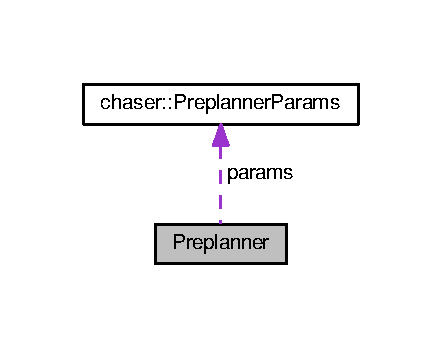
\includegraphics[width=212pt]{class_preplanner__coll__graph}
\end{center}
\end{figure}
\subsection*{Public Member Functions}
\begin{DoxyCompactItemize}
\item 
\hyperlink{class_preplanner_a4314b705278a0e3e070d5389dbb8196e}{Preplanner} ()
\item 
void \hyperlink{class_preplanner_aecde07364cbd05e2e46c95f4f5fd4951}{init} (ros\+::\+Node\+Handle nh)
\item 
void \hyperlink{class_preplanner_a6f0b709012500a44679facf0e18b985a}{preplan} (\hyperlink{struct_grid_field}{Grid\+Field} $\ast$global\+\_\+edf\+\_\+ptr, vector$<$ Point $>$ target\+\_\+pnts, Point chaser\+\_\+init)
\item 
void \hyperlink{class_preplanner_a35f3bfb85ba14d7f0c72bda1522df69e}{publish} ()
\item 
nav\+\_\+msgs\+::\+Path \hyperlink{class_preplanner_a1debbaa8e7ee64b2c22c514f89801cd1}{get\+\_\+preplanned\+\_\+waypoints} ()
\end{DoxyCompactItemize}
\subsection*{Private Member Functions}
\begin{DoxyCompactItemize}
\item 
\hyperlink{_common_8h_a225da2de31d0161f43841ed31cac064c}{Vertex\+Path} \hyperlink{class_preplanner_adff9209bb0422e7105f8bd3ed577fffd}{dijkstra} (\hyperlink{_common_8h_a1f671d518f573b692b5efa57ed576f36}{Vertex\+\_\+d} v0, \hyperlink{_common_8h_a1f671d518f573b692b5efa57ed576f36}{Vertex\+\_\+d} vf)
\item 
\hyperlink{struct_field_params}{Field\+Params} \hyperlink{class_preplanner_a5b038984427471115b1f4be24abf43b0}{get\+\_\+local\+\_\+vsf\+\_\+param\+\_\+around\+\_\+target} (Point target\+\_\+pnt)
\item 
void \hyperlink{class_preplanner_a1482068998b627fb8e2093e1eafbffd8}{compute\+\_\+visibility\+\_\+field\+\_\+seq} (\hyperlink{struct_grid_field}{Grid\+Field} $\ast$global\+\_\+edf, vector$<$ Point $>$ target\+\_\+pnts)
\item 
void \hyperlink{class_preplanner_a9404e790bfccf6563a7d947e6d11afb7}{graph\+\_\+construct} (\hyperlink{struct_grid_field}{Grid\+Field} $\ast$global\+\_\+edf, Point x0)
\item 
void \hyperlink{class_preplanner_a02321bc5136138f8aebebc494b774374}{compute\+\_\+shortest\+\_\+path} ()
\end{DoxyCompactItemize}
\subsection*{Private Attributes}
\begin{DoxyCompactItemize}
\item 
\hyperlink{structchaser_1_1_preplanner_params}{chaser\+::\+Preplanner\+Params} \hyperlink{class_preplanner_a679cc4b70f041aff73769e7ec92dc5d0}{params}
\item 
string \hyperlink{class_preplanner_a08cb79c25bd4ded139a572672e4492cd}{world\+\_\+frame\+\_\+id}
\item 
vector$<$ shared\+\_\+ptr$<$ \hyperlink{struct_grid_field}{Grid\+Field} $>$ $>$ \hyperlink{class_preplanner_aab0f91e34b86eaa581c7642ba5059308}{vsf\+\_\+field\+\_\+ptr\+\_\+seq}
\item 
\hyperlink{_common_8h_a45f376d452c699e18013842e64602733}{Graph} \hyperlink{class_preplanner_af588e8495d5e78dd5a746f7c640daa4d}{di\+\_\+graph}
\item 
\hyperlink{_common_8h_a25b10a034823d9ab576650719f0d331c}{Descriptor\+Map} \hyperlink{class_preplanner_a45603cfb24429584c4fc8bc42474e1ff}{descriptor\+\_\+map}
\item 
ros\+::\+Publisher \hyperlink{class_preplanner_a8dafcd99dc50e89404c4f33a688eba6c}{pub\+\_\+vsf\+\_\+vis}
\item 
ros\+::\+Publisher \hyperlink{class_preplanner_a9655e452a9d0e228b8c2d8cdeac8ce6b}{pub\+\_\+preplanned\+\_\+path}
\item 
ros\+::\+Publisher \hyperlink{class_preplanner_a87dc12e474ee43c9e2b095ec64ab08ce}{pub\+\_\+waypoints}
\item 
visualization\+\_\+msgs\+::\+Marker \hyperlink{class_preplanner_a9c4d6a5e43241831b0ad11bdaf99ab16}{markers\+\_\+visibility\+\_\+field\+\_\+base}
\item 
visualization\+\_\+msgs\+::\+Marker\+Array \hyperlink{class_preplanner_abcee90044b5d5935168ed132e3dfc8a6}{markers\+\_\+visibility\+\_\+field\+\_\+seq}
\item 
visualization\+\_\+msgs\+::\+Marker \hyperlink{class_preplanner_adcc96f6ec12d7cb9980aa0c889b4ccd1}{marker\+\_\+wpnts}
\item 
nav\+\_\+msgs\+::\+Path \hyperlink{class_preplanner_ace035c98e9dc23739402d346976d567b}{preplanned\+\_\+path}
\end{DoxyCompactItemize}


\subsection{Detailed Description}


\subsection{Constructor \& Destructor Documentation}
\index{Preplanner@{Preplanner}!Preplanner@{Preplanner}}
\index{Preplanner@{Preplanner}!Preplanner@{Preplanner}}
\subsubsection[{\texorpdfstring{Preplanner()}{Preplanner()}}]{\setlength{\rightskip}{0pt plus 5cm}Preplanner\+::\+Preplanner (
\begin{DoxyParamCaption}
{}
\end{DoxyParamCaption}
)}\hypertarget{class_preplanner_a4314b705278a0e3e070d5389dbb8196e}{}\label{class_preplanner_a4314b705278a0e3e070d5389dbb8196e}

\begin{DoxyCode}
3 \{\};
\end{DoxyCode}


\subsection{Member Function Documentation}
\index{Preplanner@{Preplanner}!compute\+\_\+shortest\+\_\+path@{compute\+\_\+shortest\+\_\+path}}
\index{compute\+\_\+shortest\+\_\+path@{compute\+\_\+shortest\+\_\+path}!Preplanner@{Preplanner}}
\subsubsection[{\texorpdfstring{compute\+\_\+shortest\+\_\+path()}{compute_shortest_path()}}]{\setlength{\rightskip}{0pt plus 5cm}void Preplanner\+::compute\+\_\+shortest\+\_\+path (
\begin{DoxyParamCaption}
{}
\end{DoxyParamCaption}
)\hspace{0.3cm}{\ttfamily [private]}}\hypertarget{class_preplanner_a02321bc5136138f8aebebc494b774374}{}\label{class_preplanner_a02321bc5136138f8aebebc494b774374}

\begin{DoxyCode}
303                                       \{
304 
305     ROS\_INFO(\textcolor{stringliteral}{"shortest path requested."});
306     \hyperlink{_common_8h_a225da2de31d0161f43841ed31cac064c}{VertexPath} solution\_seq = \hyperlink{class_preplanner_adff9209bb0422e7105f8bd3ed577fffd}{dijkstra}(\hyperlink{class_preplanner_a45603cfb24429584c4fc8bc42474e1ff}{descriptor\_map}[\textcolor{stringliteral}{"x0"}],
      \hyperlink{class_preplanner_a45603cfb24429584c4fc8bc42474e1ff}{descriptor\_map}[\textcolor{stringliteral}{"xf"}]);
307     \textcolor{comment}{// if path exist }
308     \textcolor{keywordflow}{if}(solution\_seq.size())\{
309 
310         solution\_seq.pop\_back();
311 
312         \textcolor{comment}{// from graph path to real path }
313         \hyperlink{class_preplanner_ace035c98e9dc23739402d346976d567b}{preplanned\_path}.poses.clear();
314         \textcolor{comment}{// marker update  }
315         \hyperlink{class_preplanner_adcc96f6ec12d7cb9980aa0c889b4ccd1}{marker\_wpnts}.points.resize(solution\_seq.size());
316         \hyperlink{class_preplanner_adcc96f6ec12d7cb9980aa0c889b4ccd1}{marker\_wpnts}.colors.resize(solution\_seq.size());  
317 
318 
319         \textcolor{keywordflow}{for}(\textcolor{keyword}{auto} it = solution\_seq.begin();it<solution\_seq.end();it++)\{
320             geometry\_msgs::PoseStamped pose\_stamped;
321 
322             pose\_stamped.pose.position = *it;
323             \hyperlink{class_preplanner_ace035c98e9dc23739402d346976d567b}{preplanned\_path}.poses.push\_back(pose\_stamped);
324 
325             \hyperlink{class_preplanner_adcc96f6ec12d7cb9980aa0c889b4ccd1}{marker\_wpnts}.colors.push\_back(\hyperlink{class_preplanner_adcc96f6ec12d7cb9980aa0c889b4ccd1}{marker\_wpnts}.color);
326             \hyperlink{class_preplanner_adcc96f6ec12d7cb9980aa0c889b4ccd1}{marker\_wpnts}.points.push\_back(*it);
327         \}
328     
329     \}
330     \textcolor{keywordflow}{else}
331         ROS\_WARN(\textcolor{stringliteral}{"[Preplanner] The preplanning couldn't be updated. (smooth planner may try to make path on
       old preplan.) "});
332     
333     
334 \}
\end{DoxyCode}
\index{Preplanner@{Preplanner}!compute\+\_\+visibility\+\_\+field\+\_\+seq@{compute\+\_\+visibility\+\_\+field\+\_\+seq}}
\index{compute\+\_\+visibility\+\_\+field\+\_\+seq@{compute\+\_\+visibility\+\_\+field\+\_\+seq}!Preplanner@{Preplanner}}
\subsubsection[{\texorpdfstring{compute\+\_\+visibility\+\_\+field\+\_\+seq(\+Grid\+Field $\ast$global\+\_\+edf, vector$<$ Point $>$ target\+\_\+pnts)}{compute_visibility_field_seq(GridField *global_edf, vector< Point > target_pnts)}}]{\setlength{\rightskip}{0pt plus 5cm}void Preplanner\+::compute\+\_\+visibility\+\_\+field\+\_\+seq (
\begin{DoxyParamCaption}
\item[{{\bf Grid\+Field} $\ast$}]{global\+\_\+edf, }
\item[{vector$<$ Point $>$}]{target\+\_\+pnts}
\end{DoxyParamCaption}
)\hspace{0.3cm}{\ttfamily [private]}}\hypertarget{class_preplanner_a1482068998b627fb8e2093e1eafbffd8}{}\label{class_preplanner_a1482068998b627fb8e2093e1eafbffd8}

\begin{DoxyCode}
92                                                                                             \{
93     \hyperlink{class_preplanner_aab0f91e34b86eaa581c7642ba5059308}{vsf\_field\_ptr\_seq}.resize(target\_pnts.size());
94     \textcolor{keywordtype}{float} numeric\_threshold = 1\hyperlink{namespace__setup__util_acdce690b925de33d6249bbbfa1109d61}{e}-2;
95     \textcolor{keywordtype}{int} t = 1;
96     \textcolor{keywordtype}{float} max\_score = -1;  \textcolor{comment}{// for visualization }
97     \textcolor{comment}{// for each target pnt}
98     \textcolor{keywordflow}{for} (\textcolor{keyword}{auto} it = target\_pnts.begin();it<target\_pnts.end();it++,t++)\{
99         
100         \textcolor{comment}{// get local conservative grid map around the current target point}
101         \textcolor{keywordtype}{int} VSF\_MODE = 1;
102         \hyperlink{class_preplanner_aab0f91e34b86eaa581c7642ba5059308}{vsf\_field\_ptr\_seq}[t-1].reset(\textcolor{keyword}{new} \hyperlink{struct_grid_field}{GridField}(
      \hyperlink{class_preplanner_a5b038984427471115b1f4be24abf43b0}{get\_local\_vsf\_param\_around\_target}(*it))); 
103         
104         \textcolor{comment}{// field value update with edf grid }
105         \textcolor{keywordflow}{for}(\textcolor{keywordtype}{int} ix = 0 ; ix<\hyperlink{class_preplanner_aab0f91e34b86eaa581c7642ba5059308}{vsf\_field\_ptr\_seq}[t-1].get()->Nx ; ix++)
106             \textcolor{keywordflow}{for}(\textcolor{keywordtype}{int} iy = 0 ; iy<\hyperlink{class_preplanner_aab0f91e34b86eaa581c7642ba5059308}{vsf\_field\_ptr\_seq}[t-1].get()->Ny ; iy++)
107                 \textcolor{keywordflow}{for}(\textcolor{keywordtype}{int} iz = 0 ; iz<\hyperlink{class_preplanner_aab0f91e34b86eaa581c7642ba5059308}{vsf\_field\_ptr\_seq}[t-1].get()->Nz ; iz++)\{
108                     
109                     \textcolor{comment}{// assign visibilty value with minimum clamping to evaluated node }
110                     Point eval\_pnt = \hyperlink{class_preplanner_aab0f91e34b86eaa581c7642ba5059308}{vsf\_field\_ptr\_seq}[t-1].get()->getCellPnt(Vector3i(ix,
      iy,iz));      
111                     \textcolor{keywordtype}{float} vs = global\_edf->\hyperlink{struct_grid_field_af9f5144af2f0cdb99784ea54c42a8516}{getRayMin}(*it,eval\_pnt,
      \hyperlink{class_preplanner_a679cc4b70f041aff73769e7ec92dc5d0}{params}.\hyperlink{structchaser_1_1_preplanner_params_a2abe7915546a5d2ebde667a1d5ccfb44}{vs\_min}); \textcolor{comment}{// visibility score from distance field                    }
112                     \hyperlink{class_preplanner_aab0f91e34b86eaa581c7642ba5059308}{vsf\_field\_ptr\_seq}[t-1].get()->field\_vals[ix][iy][iz] = vs;
113 
114                     \textcolor{comment}{// let's save the point if certain condition is satified (for graph construction)      
                }
115                     
116                     Vector3i pnt\_idx\_in\_edf = global\_edf->\hyperlink{struct_grid_field_a1a70c2de6239c1b086d01dc89b161b7c}{getCellIdx}(eval\_pnt);
117                     \textcolor{keywordtype}{float} edf\_val = global\_edf->\hyperlink{struct_grid_field_a46802a85d9533d4371d12597f0247c7d}{field\_vals}[pnt\_idx\_in\_edf(0)][pnt\_idx\_in\_edf(1)][
      pnt\_idx\_in\_edf(2)];  
118                     Vector3f bearing\_vec =(\hyperlink{_common_8h_a3e35de4eb7396984c2c5018768885d91}{geo2eigen}(eval\_pnt) - 
      \hyperlink{_common_8h_a3e35de4eb7396984c2c5018768885d91}{geo2eigen}(*it)); 
119                     \textcolor{keywordtype}{float} relative\_dist = bearing\_vec.norm();                      
120                     \textcolor{keywordtype}{float} azim = atan2(bearing\_vec(2),Vector2f(bearing\_vec(0),bearing\_vec(1)).norm());
121                     
122                     \textcolor{keywordflow}{if}(edf\_val > \hyperlink{class_preplanner_a679cc4b70f041aff73769e7ec92dc5d0}{params}.\hyperlink{structchaser_1_1_preplanner_params_a409be3b01b1b4853919d5b34e529c49a}{r\_safe} && \textcolor{comment}{// safe }
123                         relative\_dist > \hyperlink{class_preplanner_a679cc4b70f041aff73769e7ec92dc5d0}{params}.\hyperlink{structchaser_1_1_preplanner_params_aeef51c9ac61b5fa70c853463a27ff879}{d\_trakcing\_min} && \textcolor{comment}{// tracking spec}
124                         relative\_dist < \hyperlink{class_preplanner_a679cc4b70f041aff73769e7ec92dc5d0}{params}.\hyperlink{structchaser_1_1_preplanner_params_ad6659842d3039da7b064532a090651d3}{d\_trakcing\_max} && \textcolor{comment}{// tracking spec}
125                         vs > \hyperlink{class_preplanner_a679cc4b70f041aff73769e7ec92dc5d0}{params}.\hyperlink{structchaser_1_1_preplanner_params_a2abe7915546a5d2ebde667a1d5ccfb44}{vs\_min} + numeric\_threshold  && \textcolor{comment}{// non-occlusion}
126                         azim < \hyperlink{class_preplanner_a679cc4b70f041aff73769e7ec92dc5d0}{params}.\hyperlink{structchaser_1_1_preplanner_params_ab357e30646928070cd553ccf14be0beb}{max\_azim})  \textcolor{comment}{// tracking spec }
127                         \textcolor{comment}{// save}
128                         \hyperlink{class_preplanner_aab0f91e34b86eaa581c7642ba5059308}{vsf\_field\_ptr\_seq}[t-1].get()->saved\_points.push\_back(eval\_pnt);
129                     
130                     \textcolor{keywordflow}{if} (vs >= max\_score)
131                         max\_score = vs;
132 
133                 \}
134         std::cout<<\textcolor{stringliteral}{"[Preplanner] nodes at time "}<<t<<\textcolor{stringliteral}{" are "}<<\hyperlink{class_preplanner_aab0f91e34b86eaa581c7642ba5059308}{vsf\_field\_ptr\_seq}[t-1].get()
      ->saved\_points.size()<<std::endl;
135     \}
136 
137     \textcolor{comment}{// save the markers}
138 
139     \textcolor{comment}{// marker initialization     }
140     \hyperlink{class_preplanner_abcee90044b5d5935168ed132e3dfc8a6}{markers\_visibility\_field\_seq}.markers.clear();    
141 
142     \hyperlink{class_preplanner_a9c4d6a5e43241831b0ad11bdaf99ab16}{markers\_visibility\_field\_base}.header.stamp = ros::Time::now();
143     \hyperlink{class_preplanner_a9c4d6a5e43241831b0ad11bdaf99ab16}{markers\_visibility\_field\_base}.header.frame\_id = 
      \hyperlink{class_preplanner_a08cb79c25bd4ded139a572672e4492cd}{world\_frame\_id};
144     \hyperlink{class_preplanner_a9c4d6a5e43241831b0ad11bdaf99ab16}{markers\_visibility\_field\_base}.points.clear();
145     \hyperlink{class_preplanner_a9c4d6a5e43241831b0ad11bdaf99ab16}{markers\_visibility\_field\_base}.colors.clear();
146     t = 1;
147 
148     \textcolor{keywordflow}{for} (\textcolor{keyword}{auto} it = target\_pnts.begin();it<target\_pnts.end();it++,t++)\{ \textcolor{comment}{// for time}
149         \textcolor{keywordtype}{int} idx = 0;
150         \hyperlink{class_preplanner_a9c4d6a5e43241831b0ad11bdaf99ab16}{markers\_visibility\_field\_base}.ns = \textcolor{stringliteral}{"time\_"}+to\_string(t);
151 
152         \textcolor{comment}{// we draw only saved points from above }
153         \textcolor{keywordflow}{for} (\textcolor{keyword}{auto} it\_node = \hyperlink{class_preplanner_aab0f91e34b86eaa581c7642ba5059308}{vsf\_field\_ptr\_seq}[t-1].\textcolor{keyword}{get}()->saved\_points.begin() ; it\_node <
       \hyperlink{class_preplanner_aab0f91e34b86eaa581c7642ba5059308}{vsf\_field\_ptr\_seq}[t-1].get()->saved\_points.end() ; it\_node++,idx++)\{
154             Vector3i key = \hyperlink{class_preplanner_aab0f91e34b86eaa581c7642ba5059308}{vsf\_field\_ptr\_seq}[t-1].get()->getCellIdx(*it\_node);
155             \textcolor{keywordtype}{float} vs = \hyperlink{class_preplanner_aab0f91e34b86eaa581c7642ba5059308}{vsf\_field\_ptr\_seq}[t-1].get()->field\_vals[key(0)][key(1)][key(2)];
156             \textcolor{comment}{// std::cout<<vs<<std::endl;}
157             \textcolor{comment}{// marker update}
158             std\_msgs::ColorRGBA color;
159             \hyperlink{_common_8h_a75aaebf1a8b822524cc6af51a0cd83ef}{get\_color}((vs-\hyperlink{class_preplanner_a679cc4b70f041aff73769e7ec92dc5d0}{params}.\hyperlink{structchaser_1_1_preplanner_params_a2abe7915546a5d2ebde667a1d5ccfb44}{vs\_min})/(max\_score-\hyperlink{class_preplanner_a679cc4b70f041aff73769e7ec92dc5d0}{params}.
      \hyperlink{structchaser_1_1_preplanner_params_a2abe7915546a5d2ebde667a1d5ccfb44}{vs\_min}),color.r,color.g,color.b);            
160             color.a = 0.1;
161 
162             \hyperlink{class_preplanner_a9c4d6a5e43241831b0ad11bdaf99ab16}{markers\_visibility\_field\_base}.colors.push\_back(color);
163             \hyperlink{class_preplanner_a9c4d6a5e43241831b0ad11bdaf99ab16}{markers\_visibility\_field\_base}.points.push\_back(*it\_node);
164             idx ++;
165         \}
166 
167         \hyperlink{class_preplanner_abcee90044b5d5935168ed132e3dfc8a6}{markers\_visibility\_field\_seq}.markers.push\_back(
      \hyperlink{class_preplanner_a9c4d6a5e43241831b0ad11bdaf99ab16}{markers\_visibility\_field\_base});
168         \hyperlink{class_preplanner_a9c4d6a5e43241831b0ad11bdaf99ab16}{markers\_visibility\_field\_base}.points.clear();
169         \hyperlink{class_preplanner_a9c4d6a5e43241831b0ad11bdaf99ab16}{markers\_visibility\_field\_base}.colors.clear();
170         
171     \}
172 \}
\end{DoxyCode}
\index{Preplanner@{Preplanner}!dijkstra@{dijkstra}}
\index{dijkstra@{dijkstra}!Preplanner@{Preplanner}}
\subsubsection[{\texorpdfstring{dijkstra(\+Vertex\+\_\+d v0, Vertex\+\_\+d vf)}{dijkstra(Vertex_d v0, Vertex_d vf)}}]{\setlength{\rightskip}{0pt plus 5cm}{\bf Vertex\+Path} Preplanner\+::dijkstra (
\begin{DoxyParamCaption}
\item[{{\bf Vertex\+\_\+d}}]{v0, }
\item[{{\bf Vertex\+\_\+d}}]{vf}
\end{DoxyParamCaption}
)\hspace{0.3cm}{\ttfamily [private]}}\hypertarget{class_preplanner_adff9209bb0422e7105f8bd3ed577fffd}{}\label{class_preplanner_adff9209bb0422e7105f8bd3ed577fffd}

\begin{DoxyCode}
247                                                       \{
248     
249 
250 
251     \textcolor{comment}{// Create things for Dijkstra}
252     std::vector<Vertex\_d> predecessors(boost::num\_vertices(\hyperlink{class_preplanner_af588e8495d5e78dd5a746f7c640daa4d}{di\_graph})); \textcolor{comment}{// To store parents}
253     std::vector<Weight> distances(boost::num\_vertices(\hyperlink{class_preplanner_af588e8495d5e78dd5a746f7c640daa4d}{di\_graph})); \textcolor{comment}{// To store distances}
254 
255     \hyperlink{_common_8h_a7fb6309a04472de0c8cb8c74ebf92c5e}{IndexMap} indexMap = boost::get(boost::vertex\_index, \hyperlink{class_preplanner_af588e8495d5e78dd5a746f7c640daa4d}{di\_graph});
256     \hyperlink{_common_8h_a7a347729377841627777cbe0a6becbf9}{NameMap} nameMap = boost::get(boost::vertex\_name, \hyperlink{class_preplanner_af588e8495d5e78dd5a746f7c640daa4d}{di\_graph});
257 
258     \hyperlink{_common_8h_a3e372f12838999c89bb6fafe2c9b4363}{PredecessorMap} predecessorMap(&predecessors[0], indexMap);
259     \hyperlink{_common_8h_acab893c91ba1c4e4415b652ccebeea6a}{DistanceMap} distanceMap(&distances[0], indexMap);    
260 
261     boost::dijkstra\_shortest\_paths(\hyperlink{class_preplanner_af588e8495d5e78dd5a746f7c640daa4d}{di\_graph}, v0, boost::distance\_map(distanceMap).predecessor\_map(
      predecessorMap));
262 
263     \textcolor{keyword}{typedef} std::vector<Graph::edge\_descriptor> PathType;
264 
265     PathType path;
266     \hyperlink{_common_8h_a1f671d518f573b692b5efa57ed576f36}{Vertex\_d} v = vf; \textcolor{comment}{// We want to start at the destination and work our way back to the source}
267     \textcolor{keywordflow}{for}(\hyperlink{_common_8h_a1f671d518f573b692b5efa57ed576f36}{Vertex\_d} u = predecessorMap[v]; \textcolor{comment}{// Start by setting 'u' to the destintaion node's
       predecessor}
268         u != v; \textcolor{comment}{// Keep tracking the path until we get to the source}
269         v = u, u = predecessorMap[v]) \textcolor{comment}{// Set the current vertex to the current predecessor, and the
       predecessor to one level up}
270     \{
271         std::pair<Graph::edge\_descriptor, bool> edgePair = boost::edge(u, v, 
      \hyperlink{class_preplanner_af588e8495d5e78dd5a746f7c640daa4d}{di\_graph});
272         Graph::edge\_descriptor edge = edgePair.first;
273 
274         path.push\_back( edge );
275     \}
276 
277     \textcolor{keywordflow}{if} (path.size())
278     \{
279        ROS\_INFO(\textcolor{stringliteral}{"path exist"});
280         \textcolor{comment}{// Write shortest path}
281         \textcolor{keywordtype}{float} totalDistance = 0;
282 
283         \hyperlink{_common_8h_a225da2de31d0161f43841ed31cac064c}{VertexPath} vertex\_path1;
284         \hyperlink{_common_8h_a225da2de31d0161f43841ed31cac064c}{VertexPath} vertex\_path2;
285         \textcolor{keywordflow}{for}(PathType::reverse\_iterator pathIterator = path.rbegin(); pathIterator != path.rend(); ++
      pathIterator)
286         \{
287 
288 \textcolor{comment}{//            ROS\_INFO("path insertion");}
289             vertex\_path1.push\_back(nameMap[boost::source(*pathIterator, \hyperlink{class_preplanner_af588e8495d5e78dd5a746f7c640daa4d}{di\_graph})]);
290             vertex\_path2.push\_back(nameMap[boost::target(*pathIterator, \hyperlink{class_preplanner_af588e8495d5e78dd5a746f7c640daa4d}{di\_graph})]);
291         \}
292 
293         vertex\_path1.push\_back(vertex\_path2.back());
294         \textcolor{keywordflow}{return} vertex\_path1;
295     \}
296     \textcolor{keywordflow}{else}\{
297         ROS\_WARN(\textcolor{stringliteral}{"[Preplanner] path does not exist. returning zero length path. "});
298         \textcolor{keywordflow}{return} \hyperlink{_common_8h_a225da2de31d0161f43841ed31cac064c}{VertexPath}();
299     \}    
300 \}
\end{DoxyCode}
\index{Preplanner@{Preplanner}!get\+\_\+local\+\_\+vsf\+\_\+param\+\_\+around\+\_\+target@{get\+\_\+local\+\_\+vsf\+\_\+param\+\_\+around\+\_\+target}}
\index{get\+\_\+local\+\_\+vsf\+\_\+param\+\_\+around\+\_\+target@{get\+\_\+local\+\_\+vsf\+\_\+param\+\_\+around\+\_\+target}!Preplanner@{Preplanner}}
\subsubsection[{\texorpdfstring{get\+\_\+local\+\_\+vsf\+\_\+param\+\_\+around\+\_\+target(\+Point target\+\_\+pnt)}{get_local_vsf_param_around_target(Point target_pnt)}}]{\setlength{\rightskip}{0pt plus 5cm}{\bf Field\+Params} Preplanner\+::get\+\_\+local\+\_\+vsf\+\_\+param\+\_\+around\+\_\+target (
\begin{DoxyParamCaption}
\item[{Point}]{target\+\_\+pnt}
\end{DoxyParamCaption}
)\hspace{0.3cm}{\ttfamily [private]}}\hypertarget{class_preplanner_a5b038984427471115b1f4be24abf43b0}{}\label{class_preplanner_a5b038984427471115b1f4be24abf43b0}

\begin{DoxyCode}
70                                                                          \{
71 
72     \hyperlink{struct_field_params}{FieldParams} vsf\_param;    
73     \textcolor{keywordtype}{double} lx,ly,lz;
74     \textcolor{comment}{// lx = ly = 2*params.d\_trakcing\_max * cos(params.max\_azim);}
75     lx = ly = 4*\hyperlink{class_preplanner_a679cc4b70f041aff73769e7ec92dc5d0}{params}.\hyperlink{structchaser_1_1_preplanner_params_ad6659842d3039da7b064532a090651d3}{d\_trakcing\_max} ;
76     lz = \hyperlink{class_preplanner_a679cc4b70f041aff73769e7ec92dc5d0}{params}.\hyperlink{structchaser_1_1_preplanner_params_ad6659842d3039da7b064532a090651d3}{d\_trakcing\_max} * sin(\hyperlink{class_preplanner_a679cc4b70f041aff73769e7ec92dc5d0}{params}.\hyperlink{structchaser_1_1_preplanner_params_ab357e30646928070cd553ccf14be0beb}{max\_azim}) - 
      \hyperlink{class_preplanner_a679cc4b70f041aff73769e7ec92dc5d0}{params}.\hyperlink{structchaser_1_1_preplanner_params_aeef51c9ac61b5fa70c853463a27ff879}{d\_trakcing\_min} * sin(\hyperlink{class_preplanner_a679cc4b70f041aff73769e7ec92dc5d0}{params}.\hyperlink{structchaser_1_1_preplanner_params_aa6846dd2e2d69d5f0d5a9b30710db6e1}{min\_azim}) ;
77 
78     vsf\_param.\hyperlink{struct_field_params_ae702824fca4d3a4b4bbf4ac90084e3a7}{x0} = target\_pnt.x - lx/2;
79     vsf\_param.\hyperlink{struct_field_params_ae9d400dadcfaaff44706adae06664c83}{y0} = target\_pnt.y - ly/2;
80     vsf\_param.\hyperlink{struct_field_params_a51178f64cc93a37d6d8f774228c24a0f}{z0} = target\_pnt.z;
81     vsf\_param.\hyperlink{struct_field_params_a9738077907a76512e49cb284ee3f1949}{lx} = lx;
82     vsf\_param.\hyperlink{struct_field_params_afb39ded77b5714992e9b2f8c5d735d30}{ly} = ly;
83     vsf\_param.\hyperlink{struct_field_params_ae7532b58aed59f5b47233e57b67acc1a}{lz} = lz;
84     
85     vsf\_param.\hyperlink{struct_field_params_a520406c76b3abf392401626bc2161370}{resolution} = \hyperlink{class_preplanner_a679cc4b70f041aff73769e7ec92dc5d0}{params}.\hyperlink{structchaser_1_1_preplanner_params_ac30a8ee32bae78f84b863234853f6497}{vsf\_resolution};
86     vsf\_param.\hyperlink{struct_field_params_ae6eabaa6e593c9dbac48b2f96bea80ec}{ray\_stride\_res} =  \hyperlink{class_preplanner_a679cc4b70f041aff73769e7ec92dc5d0}{params}.\hyperlink{structchaser_1_1_preplanner_params_ac30a8ee32bae78f84b863234853f6497}{vsf\_resolution}; \textcolor{comment}{// not used for
       vsf grid }
87 
88     \textcolor{keywordflow}{return} vsf\_param;
89 \};
\end{DoxyCode}
\index{Preplanner@{Preplanner}!get\+\_\+preplanned\+\_\+waypoints@{get\+\_\+preplanned\+\_\+waypoints}}
\index{get\+\_\+preplanned\+\_\+waypoints@{get\+\_\+preplanned\+\_\+waypoints}!Preplanner@{Preplanner}}
\subsubsection[{\texorpdfstring{get\+\_\+preplanned\+\_\+waypoints()}{get_preplanned_waypoints()}}]{\setlength{\rightskip}{0pt plus 5cm}nav\+\_\+msgs\+::\+Path Preplanner\+::get\+\_\+preplanned\+\_\+waypoints (
\begin{DoxyParamCaption}
{}
\end{DoxyParamCaption}
)}\hypertarget{class_preplanner_a1debbaa8e7ee64b2c22c514f89801cd1}{}\label{class_preplanner_a1debbaa8e7ee64b2c22c514f89801cd1}

\begin{DoxyCode}
350 \{\textcolor{keywordflow}{return} \hyperlink{class_preplanner_ace035c98e9dc23739402d346976d567b}{preplanned\_path};\}
\end{DoxyCode}
\index{Preplanner@{Preplanner}!graph\+\_\+construct@{graph\+\_\+construct}}
\index{graph\+\_\+construct@{graph\+\_\+construct}!Preplanner@{Preplanner}}
\subsubsection[{\texorpdfstring{graph\+\_\+construct(\+Grid\+Field $\ast$global\+\_\+edf, Point x0)}{graph_construct(GridField *global_edf, Point x0)}}]{\setlength{\rightskip}{0pt plus 5cm}void Preplanner\+::graph\+\_\+construct (
\begin{DoxyParamCaption}
\item[{{\bf Grid\+Field} $\ast$}]{global\+\_\+edf, }
\item[{Point}]{x0}
\end{DoxyParamCaption}
)\hspace{0.3cm}{\ttfamily [private]}}\hypertarget{class_preplanner_a9404e790bfccf6563a7d947e6d11afb7}{}\label{class_preplanner_a9404e790bfccf6563a7d947e6d11afb7}

\begin{DoxyCode}
175                                                               \{
176     
177     \textcolor{comment}{// init graph with the initial position of chaser }
178     \hyperlink{class_preplanner_af588e8495d5e78dd5a746f7c640daa4d}{di\_graph} = \hyperlink{_common_8h_a45f376d452c699e18013842e64602733}{Graph}();
179     \hyperlink{class_preplanner_a45603cfb24429584c4fc8bc42474e1ff}{descriptor\_map}.clear();
180     
181     vector<Node<Point>> prev\_layer;
182     \hyperlink{struct_node}{Node<Point>} initial\_node; initial\_node.\hyperlink{struct_node_a01b9071c0de774c720b64583262d1559}{value} = x0; initial\_node.
      \hyperlink{struct_node_a795bdc93cbf63ccddcdf2168d858492c}{name} = \textcolor{stringliteral}{"x0"};
183     prev\_layer.push\_back(initial\_node);
184     
185     \hyperlink{_common_8h_a1f671d518f573b692b5efa57ed576f36}{Vertex\_d} v0 = boost::add\_vertex(x0,\hyperlink{class_preplanner_af588e8495d5e78dd5a746f7c640daa4d}{di\_graph});
186     \hyperlink{class_preplanner_a45603cfb24429584c4fc8bc42474e1ff}{descriptor\_map}.insert(make\_pair(\hyperlink{_common_8h_a817e52d0171d1503034d4cbe7fd89a1b}{VertexName}(\textcolor{stringliteral}{"x0"}),v0));
187  
188     \textcolor{keywordtype}{int} H = \hyperlink{class_preplanner_aab0f91e34b86eaa581c7642ba5059308}{vsf\_field\_ptr\_seq}.size(); \textcolor{comment}{// total prediction horizon }
189     \textcolor{keywordtype}{int} N\_edge = 0; 
190     \textcolor{keywordtype}{int} N\_edge\_sub = 0;
191 
192     \textcolor{comment}{// in case of t = 0, we don't need (just current step). }
193     \textcolor{keywordflow}{for}(\textcolor{keywordtype}{int} t = 1; t<H;t++)\{
194         N\_edge\_sub = 0;
195         \hyperlink{struct_grid_field}{GridField}* cur\_vsf\_ptr = \hyperlink{class_preplanner_aab0f91e34b86eaa581c7642ba5059308}{vsf\_field\_ptr\_seq}[t].get();        
196         vector<Node<Point>> cur\_layer = cur\_vsf\_ptr->\hyperlink{struct_grid_field_acd8fd9f0893ad94aa4f20b4b4d81802a}{generate\_node}(t); \textcolor{comment}{// current layer   }
197 
198         \textcolor{keywordflow}{for} (\textcolor{keyword}{auto} it\_cur = cur\_layer.begin() ; it\_cur<cur\_layer.end(); it\_cur++)\{
199             
200             \textcolor{comment}{// step1 :  let's register the node(pnt,name) in the current layer into graph }
201             Point cur\_pnt = it\_cur->value; Vector3f cur\_vec = \hyperlink{_common_8h_a3e35de4eb7396984c2c5018768885d91}{geo2eigen}(cur\_pnt); 
202             \hyperlink{_common_8h_a1f671d518f573b692b5efa57ed576f36}{Vertex\_d} cur\_vert = boost::add\_vertex(cur\_pnt,\hyperlink{class_preplanner_af588e8495d5e78dd5a746f7c640daa4d}{di\_graph});
203             \hyperlink{class_preplanner_a45603cfb24429584c4fc8bc42474e1ff}{descriptor\_map}.insert(make\_pair(it\_cur->name,cur\_vert));
204             
205             \textcolor{comment}{// call the previous layer  }
206             \hyperlink{struct_grid_field}{GridField}* prev\_vsf\_ptr = \hyperlink{class_preplanner_aab0f91e34b86eaa581c7642ba5059308}{vsf\_field\_ptr\_seq}[t-1].get();              
                
207             
208             \textcolor{comment}{// step2 : let's connect with previous layer and add edges }
209             \textcolor{keywordflow}{for}(\textcolor{keyword}{auto} it\_prev = prev\_layer.begin(); it\_prev < prev\_layer.end();it\_prev++)\{ \textcolor{comment}{// prev\_layer }
210                 \hyperlink{_common_8h_a1f671d518f573b692b5efa57ed576f36}{Vertex\_d} prev\_vert = \hyperlink{class_preplanner_a45603cfb24429584c4fc8bc42474e1ff}{descriptor\_map}[it\_prev->name];
211                 Point prev\_pnt = it\_prev->value; Vector3f prev\_vec = \hyperlink{_common_8h_a3e35de4eb7396984c2c5018768885d91}{geo2eigen}(prev\_pnt);
212 
213                 \textcolor{comment}{// this condition should be satisfied to be connected }
214                 \textcolor{keywordflow}{if}(((cur\_vec-prev\_vec).norm() < \hyperlink{class_preplanner_a679cc4b70f041aff73769e7ec92dc5d0}{params}.\hyperlink{structchaser_1_1_preplanner_params_a90021bd30b7e88b50cf9317ff3673482}{d\_connect\_max}) && (global\_edf->
      \hyperlink{struct_grid_field_af9f5144af2f0cdb99784ea54c42a8516}{getRayMin}(cur\_pnt,prev\_pnt,0) > \hyperlink{class_preplanner_a679cc4b70f041aff73769e7ec92dc5d0}{params}.\hyperlink{structchaser_1_1_preplanner_params_a409be3b01b1b4853919d5b34e529c49a}{r\_safe}) )\{
215                     \textcolor{keywordtype}{float} weight = (cur\_vec-prev\_vec).norm() + 
216                             \hyperlink{class_preplanner_a679cc4b70f041aff73769e7ec92dc5d0}{params}.\hyperlink{structchaser_1_1_preplanner_params_a1778793e5b16806c867291c1a5471a04}{w\_v}*1/sqrt(cur\_vsf\_ptr->\hyperlink{struct_grid_field_a3e49ca50129cb18db833bd4168c5d254}{getRayMean}(cur\_pnt,prev\_pnt) 
      * prev\_vsf\_ptr->\hyperlink{struct_grid_field_a3e49ca50129cb18db833bd4168c5d254}{getRayMean}(prev\_pnt,cur\_pnt)) 
217                             + \hyperlink{class_preplanner_a679cc4b70f041aff73769e7ec92dc5d0}{params}.\hyperlink{structchaser_1_1_preplanner_params_ae443edaa7e2912a6a7643272305c91f5}{w\_d}*abs((\hyperlink{_common_8h_a3e35de4eb7396984c2c5018768885d91}{geo2eigen}(cur\_vsf\_ptr->
      \hyperlink{struct_grid_field_aacd39f9388090694e5c428cc612fd887}{getCentre}()) - cur\_vec).norm() - \hyperlink{class_preplanner_a679cc4b70f041aff73769e7ec92dc5d0}{params}.\hyperlink{structchaser_1_1_preplanner_params_a6a950244cbb256abb9a4e93388c0177f}{d\_trakcing\_des});                     
218                     boost::add\_edge(prev\_vert,cur\_vert,weight,\hyperlink{class_preplanner_af588e8495d5e78dd5a746f7c640daa4d}{di\_graph});
219                     \textcolor{keywordflow}{if}(weight <1\hyperlink{namespace__setup__util_acdce690b925de33d6249bbbfa1109d61}{e}-4)
220                         ROS\_WARN(\textcolor{stringliteral}{"weight is zero"});
221                     N\_edge ++;
222                     N\_edge\_sub++;
223                 \}
224             \}            
225         \}
226         prev\_layer = cur\_layer;
227         cout<<\textcolor{stringliteral}{"[Preplanner] connected edge to this layer: "}<<N\_edge\_sub<<std::endl;
228     \}
229     
230     cout<<\textcolor{stringliteral}{"[Preplanner] total number of edges "}<<N\_edge<<std::endl;
231 
232 
233     \textcolor{comment}{// graph finishing }
234 
235     \hyperlink{struct_grid_field}{GridField}* prev\_vsf\_ptr = \hyperlink{class_preplanner_aab0f91e34b86eaa581c7642ba5059308}{vsf\_field\_ptr\_seq}[H-1].get();
236     \hyperlink{_common_8h_a1f671d518f573b692b5efa57ed576f36}{Vertex\_d} vf = boost::add\_vertex(Point(),\hyperlink{class_preplanner_af588e8495d5e78dd5a746f7c640daa4d}{di\_graph});
237     \hyperlink{class_preplanner_a45603cfb24429584c4fc8bc42474e1ff}{descriptor\_map}.insert(make\_pair(\hyperlink{_common_8h_a817e52d0171d1503034d4cbe7fd89a1b}{VertexName}(\textcolor{stringliteral}{"xf"}),vf));
238 
239     \textcolor{comment}{// step2 : let's connect with previous layer }
240     \textcolor{keywordflow}{for}(\textcolor{keyword}{auto} it\_prev = prev\_layer.begin(); it\_prev < prev\_layer.end();it\_prev++)\{ \textcolor{comment}{// prev\_layer }
241         \hyperlink{_common_8h_a1f671d518f573b692b5efa57ed576f36}{Vertex\_d} prev\_vert = \hyperlink{class_preplanner_a45603cfb24429584c4fc8bc42474e1ff}{descriptor\_map}[it\_prev->name];
242         \textcolor{comment}{// this condition should be satisfied to be connected }
243             boost::add\_edge(prev\_vert,vf,0,\hyperlink{class_preplanner_af588e8495d5e78dd5a746f7c640daa4d}{di\_graph});
244     \}
245 \}
\end{DoxyCode}
\index{Preplanner@{Preplanner}!init@{init}}
\index{init@{init}!Preplanner@{Preplanner}}
\subsubsection[{\texorpdfstring{init(ros\+::\+Node\+Handle nh)}{init(ros::NodeHandle nh)}}]{\setlength{\rightskip}{0pt plus 5cm}void Preplanner\+::init (
\begin{DoxyParamCaption}
\item[{ros\+::\+Node\+Handle}]{nh}
\end{DoxyParamCaption}
)}\hypertarget{class_preplanner_aecde07364cbd05e2e46c95f4f5fd4951}{}\label{class_preplanner_aecde07364cbd05e2e46c95f4f5fd4951}

\begin{DoxyCode}
5                                      \{
6 
7     \textcolor{comment}{// preplanner params parsing }
8     nh.param(\textcolor{stringliteral}{"w\_v"},\hyperlink{class_preplanner_a679cc4b70f041aff73769e7ec92dc5d0}{params}.\hyperlink{structchaser_1_1_preplanner_params_a1778793e5b16806c867291c1a5471a04}{w\_v},5.0);       
9     nh.param(\textcolor{stringliteral}{"w\_d"},\hyperlink{class_preplanner_a679cc4b70f041aff73769e7ec92dc5d0}{params}.\hyperlink{structchaser_1_1_preplanner_params_ae443edaa7e2912a6a7643272305c91f5}{w\_d},1.5);            
10     nh.param(\textcolor{stringliteral}{"r\_safe"},\hyperlink{class_preplanner_a679cc4b70f041aff73769e7ec92dc5d0}{params}.\hyperlink{structchaser_1_1_preplanner_params_a409be3b01b1b4853919d5b34e529c49a}{r\_safe},0.5);
11     nh.param(\textcolor{stringliteral}{"min\_z"},\hyperlink{class_preplanner_a679cc4b70f041aff73769e7ec92dc5d0}{params}.\hyperlink{structchaser_1_1_preplanner_params_ad23cd70894c614834c2a80e35de3e373}{min\_z},0.4);
12     nh.param(\textcolor{stringliteral}{"vs\_min"},\hyperlink{class_preplanner_a679cc4b70f041aff73769e7ec92dc5d0}{params}.\hyperlink{structchaser_1_1_preplanner_params_a2abe7915546a5d2ebde667a1d5ccfb44}{vs\_min},0.3);
13     nh.param(\textcolor{stringliteral}{"vsf\_resolution"},\hyperlink{class_preplanner_a679cc4b70f041aff73769e7ec92dc5d0}{params}.\hyperlink{structchaser_1_1_preplanner_params_ac30a8ee32bae78f84b863234853f6497}{vsf\_resolution},0.7);
14     nh.param(\textcolor{stringliteral}{"d\_connect\_max"},\hyperlink{class_preplanner_a679cc4b70f041aff73769e7ec92dc5d0}{params}.\hyperlink{structchaser_1_1_preplanner_params_a90021bd30b7e88b50cf9317ff3673482}{d\_connect\_max},2.5);
15 
16     nh.param(\textcolor{stringliteral}{"max\_tracking\_distance"},\hyperlink{class_preplanner_a679cc4b70f041aff73769e7ec92dc5d0}{params}.\hyperlink{structchaser_1_1_preplanner_params_ad6659842d3039da7b064532a090651d3}{d\_trakcing\_max},4.0);
17     nh.param(\textcolor{stringliteral}{"min\_tracking\_distance"},\hyperlink{class_preplanner_a679cc4b70f041aff73769e7ec92dc5d0}{params}.\hyperlink{structchaser_1_1_preplanner_params_aeef51c9ac61b5fa70c853463a27ff879}{d\_trakcing\_min},1.0);
18     nh.param(\textcolor{stringliteral}{"des\_tracking\_distance"},\hyperlink{class_preplanner_a679cc4b70f041aff73769e7ec92dc5d0}{params}.\hyperlink{structchaser_1_1_preplanner_params_a6a950244cbb256abb9a4e93388c0177f}{d\_trakcing\_des},2.5);
19     nh.param(\textcolor{stringliteral}{"max\_azim"},\hyperlink{class_preplanner_a679cc4b70f041aff73769e7ec92dc5d0}{params}.\hyperlink{structchaser_1_1_preplanner_params_ab357e30646928070cd553ccf14be0beb}{max\_azim},(3.141592/4));
20     nh.param(\textcolor{stringliteral}{"min\_azim"},\hyperlink{class_preplanner_a679cc4b70f041aff73769e7ec92dc5d0}{params}.\hyperlink{structchaser_1_1_preplanner_params_aa6846dd2e2d69d5f0d5a9b30710db6e1}{min\_azim},(3.141592/7));
21 
22 
23     \textcolor{comment}{// world\_frame\_id }
24     nh.param<\textcolor{keywordtype}{string}>(\textcolor{stringliteral}{"world\_frame\_id"},\hyperlink{class_preplanner_a08cb79c25bd4ded139a572672e4492cd}{world\_frame\_id},\textcolor{stringliteral}{"/world"});
25     nh.param<\textcolor{keywordtype}{string}>(\textcolor{stringliteral}{"world\_frame\_id"},\hyperlink{class_preplanner_a9c4d6a5e43241831b0ad11bdaf99ab16}{markers\_visibility\_field\_base}.header.
      frame\_id,\textcolor{stringliteral}{"/world"});
26     nh.param<\textcolor{keywordtype}{string}>(\textcolor{stringliteral}{"world\_frame\_id"},\hyperlink{class_preplanner_ace035c98e9dc23739402d346976d567b}{preplanned\_path}.header.frame\_id,\textcolor{stringliteral}{"/world"});
27 
28     \textcolor{comment}{// marker initialize }
29     
30     \textcolor{comment}{// waypoints }
31     \hyperlink{class_preplanner_adcc96f6ec12d7cb9980aa0c889b4ccd1}{marker\_wpnts}.header.frame\_id = \hyperlink{class_preplanner_a9c4d6a5e43241831b0ad11bdaf99ab16}{markers\_visibility\_field\_base}.
      header.frame\_id;
32     \hyperlink{class_preplanner_adcc96f6ec12d7cb9980aa0c889b4ccd1}{marker\_wpnts}.ns = \textcolor{stringliteral}{"waypoints"};
33     \hyperlink{class_preplanner_adcc96f6ec12d7cb9980aa0c889b4ccd1}{marker\_wpnts}.id = 0;
34     \hyperlink{class_preplanner_adcc96f6ec12d7cb9980aa0c889b4ccd1}{marker\_wpnts}.type = visualization\_msgs::Marker::SPHERE\_LIST;
35     \hyperlink{class_preplanner_adcc96f6ec12d7cb9980aa0c889b4ccd1}{marker\_wpnts}.color.r = 14.0/255.0;
36     \hyperlink{class_preplanner_adcc96f6ec12d7cb9980aa0c889b4ccd1}{marker\_wpnts}.color.g = 50.0/255.0;
37     \hyperlink{class_preplanner_adcc96f6ec12d7cb9980aa0c889b4ccd1}{marker\_wpnts}.color.b = 1.0;
38     \hyperlink{class_preplanner_adcc96f6ec12d7cb9980aa0c889b4ccd1}{marker\_wpnts}.color.a = 0.3;
39     \hyperlink{class_preplanner_adcc96f6ec12d7cb9980aa0c889b4ccd1}{marker\_wpnts}.pose.orientation.w = 1.0;
40     \textcolor{keywordtype}{double} scale = 0.08; 
41     \hyperlink{class_preplanner_adcc96f6ec12d7cb9980aa0c889b4ccd1}{marker\_wpnts}.scale.x = scale;
42     \hyperlink{class_preplanner_adcc96f6ec12d7cb9980aa0c889b4ccd1}{marker\_wpnts}.scale.y = scale;
43     \hyperlink{class_preplanner_adcc96f6ec12d7cb9980aa0c889b4ccd1}{marker\_wpnts}.scale.z = scale;    
44 
45     \textcolor{comment}{// vsf\_grid\_seq }
46 
47     \textcolor{comment}{// marker base}
48     visualization\_msgs::Marker marker;
49     marker.header.frame\_id = \hyperlink{class_preplanner_a9c4d6a5e43241831b0ad11bdaf99ab16}{markers\_visibility\_field\_base}.header.frame\_id;;
50     marker.action = visualization\_msgs::Marker::ADD;
51     marker.type = visualization\_msgs::Marker::CUBE\_LIST;      
52     marker.pose.orientation.x = 0;
53     marker.pose.orientation.y = 0;
54     marker.pose.orientation.z = 0;
55     marker.pose.orientation.w = 1;                  
56     marker.scale.x = \hyperlink{class_preplanner_a679cc4b70f041aff73769e7ec92dc5d0}{params}.\hyperlink{structchaser_1_1_preplanner_params_ac30a8ee32bae78f84b863234853f6497}{vsf\_resolution};
57     marker.scale.y = \hyperlink{class_preplanner_a679cc4b70f041aff73769e7ec92dc5d0}{params}.\hyperlink{structchaser_1_1_preplanner_params_ac30a8ee32bae78f84b863234853f6497}{vsf\_resolution};
58     marker.scale.z = \hyperlink{class_preplanner_a679cc4b70f041aff73769e7ec92dc5d0}{params}.\hyperlink{structchaser_1_1_preplanner_params_ac30a8ee32bae78f84b863234853f6497}{vsf\_resolution};
59     \hyperlink{class_preplanner_a9c4d6a5e43241831b0ad11bdaf99ab16}{markers\_visibility\_field\_base} = marker; 
60 
61 
62     \textcolor{comment}{// ros initialize }
63     \hyperlink{class_preplanner_a8dafcd99dc50e89404c4f33a688eba6c}{pub\_vsf\_vis} = nh.advertise<visualization\_msgs::MarkerArray>(\textcolor{stringliteral}{"vsf\_grid\_seq"},1);
64     \hyperlink{class_preplanner_a87dc12e474ee43c9e2b095ec64ab08ce}{pub\_waypoints} = nh.advertise<visualization\_msgs::Marker>(\textcolor{stringliteral}{"preplanned\_waypoints"},1);    
65     \hyperlink{class_preplanner_a9655e452a9d0e228b8c2d8cdeac8ce6b}{pub\_preplanned\_path} = nh.advertise<nav\_msgs::Path>(\textcolor{stringliteral}{"preplanned\_path"},1);
66 
67 
68 \};
\end{DoxyCode}
\index{Preplanner@{Preplanner}!preplan@{preplan}}
\index{preplan@{preplan}!Preplanner@{Preplanner}}
\subsubsection[{\texorpdfstring{preplan(\+Grid\+Field $\ast$global\+\_\+edf\+\_\+ptr, vector$<$ Point $>$ target\+\_\+pnts, Point chaser\+\_\+init)}{preplan(GridField *global_edf_ptr, vector< Point > target_pnts, Point chaser_init)}}]{\setlength{\rightskip}{0pt plus 5cm}void Preplanner\+::preplan (
\begin{DoxyParamCaption}
\item[{{\bf Grid\+Field} $\ast$}]{global\+\_\+edf\+\_\+ptr, }
\item[{vector$<$ Point $>$}]{target\+\_\+pnts, }
\item[{Point}]{chaser\+\_\+init}
\end{DoxyParamCaption}
)}\hypertarget{class_preplanner_a6f0b709012500a44679facf0e18b985a}{}\label{class_preplanner_a6f0b709012500a44679facf0e18b985a}

\begin{DoxyCode}
337                                                                                          \{
338 
339 
340 
341     \textcolor{comment}{// set the height of the moving target }
342     \textcolor{keywordflow}{for}(\textcolor{keyword}{auto} it = target\_pnts.begin(); it<target\_pnts.end(); it++)
343         it->z = \hyperlink{class_preplanner_a679cc4b70f041aff73769e7ec92dc5d0}{params}.\hyperlink{structchaser_1_1_preplanner_params_ad23cd70894c614834c2a80e35de3e373}{min\_z} + 1\hyperlink{namespace__setup__util_acdce690b925de33d6249bbbfa1109d61}{e}-3;
344 
345     \hyperlink{class_preplanner_a1482068998b627fb8e2093e1eafbffd8}{compute\_visibility\_field\_seq}(global\_edf,target\_pnts);  
346     \hyperlink{class_preplanner_a9404e790bfccf6563a7d947e6d11afb7}{graph\_construct}(global\_edf,chaser\_init);        
347     \hyperlink{class_preplanner_a02321bc5136138f8aebebc494b774374}{compute\_shortest\_path}();   
348 \}
\end{DoxyCode}
\index{Preplanner@{Preplanner}!publish@{publish}}
\index{publish@{publish}!Preplanner@{Preplanner}}
\subsubsection[{\texorpdfstring{publish()}{publish()}}]{\setlength{\rightskip}{0pt plus 5cm}void Preplanner\+::publish (
\begin{DoxyParamCaption}
{}
\end{DoxyParamCaption}
)}\hypertarget{class_preplanner_a35f3bfb85ba14d7f0c72bda1522df69e}{}\label{class_preplanner_a35f3bfb85ba14d7f0c72bda1522df69e}

\begin{DoxyCode}
352                         \{
353     \textcolor{comment}{// vsf seq}
354     \hyperlink{class_preplanner_a8dafcd99dc50e89404c4f33a688eba6c}{pub\_vsf\_vis}.publish(\hyperlink{class_preplanner_abcee90044b5d5935168ed132e3dfc8a6}{markers\_visibility\_field\_seq});
355     \textcolor{comment}{// waypoints}
356     \hyperlink{class_preplanner_a87dc12e474ee43c9e2b095ec64ab08ce}{pub\_waypoints}.publish(\hyperlink{class_preplanner_adcc96f6ec12d7cb9980aa0c889b4ccd1}{marker\_wpnts});
357     \textcolor{comment}{// preplanned path }
358     \hyperlink{class_preplanner_a9655e452a9d0e228b8c2d8cdeac8ce6b}{pub\_preplanned\_path}.publish(\hyperlink{class_preplanner_ace035c98e9dc23739402d346976d567b}{preplanned\_path});
359 \}\end{DoxyCode}


\subsection{Member Data Documentation}
\index{Preplanner@{Preplanner}!descriptor\+\_\+map@{descriptor\+\_\+map}}
\index{descriptor\+\_\+map@{descriptor\+\_\+map}!Preplanner@{Preplanner}}
\subsubsection[{\texorpdfstring{descriptor\+\_\+map}{descriptor_map}}]{\setlength{\rightskip}{0pt plus 5cm}{\bf Descriptor\+Map} Preplanner\+::descriptor\+\_\+map\hspace{0.3cm}{\ttfamily [private]}}\hypertarget{class_preplanner_a45603cfb24429584c4fc8bc42474e1ff}{}\label{class_preplanner_a45603cfb24429584c4fc8bc42474e1ff}
\index{Preplanner@{Preplanner}!di\+\_\+graph@{di\+\_\+graph}}
\index{di\+\_\+graph@{di\+\_\+graph}!Preplanner@{Preplanner}}
\subsubsection[{\texorpdfstring{di\+\_\+graph}{di_graph}}]{\setlength{\rightskip}{0pt plus 5cm}{\bf Graph} Preplanner\+::di\+\_\+graph\hspace{0.3cm}{\ttfamily [private]}}\hypertarget{class_preplanner_af588e8495d5e78dd5a746f7c640daa4d}{}\label{class_preplanner_af588e8495d5e78dd5a746f7c640daa4d}
\index{Preplanner@{Preplanner}!marker\+\_\+wpnts@{marker\+\_\+wpnts}}
\index{marker\+\_\+wpnts@{marker\+\_\+wpnts}!Preplanner@{Preplanner}}
\subsubsection[{\texorpdfstring{marker\+\_\+wpnts}{marker_wpnts}}]{\setlength{\rightskip}{0pt plus 5cm}visualization\+\_\+msgs\+::\+Marker Preplanner\+::marker\+\_\+wpnts\hspace{0.3cm}{\ttfamily [private]}}\hypertarget{class_preplanner_adcc96f6ec12d7cb9980aa0c889b4ccd1}{}\label{class_preplanner_adcc96f6ec12d7cb9980aa0c889b4ccd1}
\index{Preplanner@{Preplanner}!markers\+\_\+visibility\+\_\+field\+\_\+base@{markers\+\_\+visibility\+\_\+field\+\_\+base}}
\index{markers\+\_\+visibility\+\_\+field\+\_\+base@{markers\+\_\+visibility\+\_\+field\+\_\+base}!Preplanner@{Preplanner}}
\subsubsection[{\texorpdfstring{markers\+\_\+visibility\+\_\+field\+\_\+base}{markers_visibility_field_base}}]{\setlength{\rightskip}{0pt plus 5cm}visualization\+\_\+msgs\+::\+Marker Preplanner\+::markers\+\_\+visibility\+\_\+field\+\_\+base\hspace{0.3cm}{\ttfamily [private]}}\hypertarget{class_preplanner_a9c4d6a5e43241831b0ad11bdaf99ab16}{}\label{class_preplanner_a9c4d6a5e43241831b0ad11bdaf99ab16}
\index{Preplanner@{Preplanner}!markers\+\_\+visibility\+\_\+field\+\_\+seq@{markers\+\_\+visibility\+\_\+field\+\_\+seq}}
\index{markers\+\_\+visibility\+\_\+field\+\_\+seq@{markers\+\_\+visibility\+\_\+field\+\_\+seq}!Preplanner@{Preplanner}}
\subsubsection[{\texorpdfstring{markers\+\_\+visibility\+\_\+field\+\_\+seq}{markers_visibility_field_seq}}]{\setlength{\rightskip}{0pt plus 5cm}visualization\+\_\+msgs\+::\+Marker\+Array Preplanner\+::markers\+\_\+visibility\+\_\+field\+\_\+seq\hspace{0.3cm}{\ttfamily [private]}}\hypertarget{class_preplanner_abcee90044b5d5935168ed132e3dfc8a6}{}\label{class_preplanner_abcee90044b5d5935168ed132e3dfc8a6}
\index{Preplanner@{Preplanner}!params@{params}}
\index{params@{params}!Preplanner@{Preplanner}}
\subsubsection[{\texorpdfstring{params}{params}}]{\setlength{\rightskip}{0pt plus 5cm}{\bf chaser\+::\+Preplanner\+Params} Preplanner\+::params\hspace{0.3cm}{\ttfamily [private]}}\hypertarget{class_preplanner_a679cc4b70f041aff73769e7ec92dc5d0}{}\label{class_preplanner_a679cc4b70f041aff73769e7ec92dc5d0}
\index{Preplanner@{Preplanner}!preplanned\+\_\+path@{preplanned\+\_\+path}}
\index{preplanned\+\_\+path@{preplanned\+\_\+path}!Preplanner@{Preplanner}}
\subsubsection[{\texorpdfstring{preplanned\+\_\+path}{preplanned_path}}]{\setlength{\rightskip}{0pt plus 5cm}nav\+\_\+msgs\+::\+Path Preplanner\+::preplanned\+\_\+path\hspace{0.3cm}{\ttfamily [private]}}\hypertarget{class_preplanner_ace035c98e9dc23739402d346976d567b}{}\label{class_preplanner_ace035c98e9dc23739402d346976d567b}
\index{Preplanner@{Preplanner}!pub\+\_\+preplanned\+\_\+path@{pub\+\_\+preplanned\+\_\+path}}
\index{pub\+\_\+preplanned\+\_\+path@{pub\+\_\+preplanned\+\_\+path}!Preplanner@{Preplanner}}
\subsubsection[{\texorpdfstring{pub\+\_\+preplanned\+\_\+path}{pub_preplanned_path}}]{\setlength{\rightskip}{0pt plus 5cm}ros\+::\+Publisher Preplanner\+::pub\+\_\+preplanned\+\_\+path\hspace{0.3cm}{\ttfamily [private]}}\hypertarget{class_preplanner_a9655e452a9d0e228b8c2d8cdeac8ce6b}{}\label{class_preplanner_a9655e452a9d0e228b8c2d8cdeac8ce6b}
\index{Preplanner@{Preplanner}!pub\+\_\+vsf\+\_\+vis@{pub\+\_\+vsf\+\_\+vis}}
\index{pub\+\_\+vsf\+\_\+vis@{pub\+\_\+vsf\+\_\+vis}!Preplanner@{Preplanner}}
\subsubsection[{\texorpdfstring{pub\+\_\+vsf\+\_\+vis}{pub_vsf_vis}}]{\setlength{\rightskip}{0pt plus 5cm}ros\+::\+Publisher Preplanner\+::pub\+\_\+vsf\+\_\+vis\hspace{0.3cm}{\ttfamily [private]}}\hypertarget{class_preplanner_a8dafcd99dc50e89404c4f33a688eba6c}{}\label{class_preplanner_a8dafcd99dc50e89404c4f33a688eba6c}
\index{Preplanner@{Preplanner}!pub\+\_\+waypoints@{pub\+\_\+waypoints}}
\index{pub\+\_\+waypoints@{pub\+\_\+waypoints}!Preplanner@{Preplanner}}
\subsubsection[{\texorpdfstring{pub\+\_\+waypoints}{pub_waypoints}}]{\setlength{\rightskip}{0pt plus 5cm}ros\+::\+Publisher Preplanner\+::pub\+\_\+waypoints\hspace{0.3cm}{\ttfamily [private]}}\hypertarget{class_preplanner_a87dc12e474ee43c9e2b095ec64ab08ce}{}\label{class_preplanner_a87dc12e474ee43c9e2b095ec64ab08ce}
\index{Preplanner@{Preplanner}!vsf\+\_\+field\+\_\+ptr\+\_\+seq@{vsf\+\_\+field\+\_\+ptr\+\_\+seq}}
\index{vsf\+\_\+field\+\_\+ptr\+\_\+seq@{vsf\+\_\+field\+\_\+ptr\+\_\+seq}!Preplanner@{Preplanner}}
\subsubsection[{\texorpdfstring{vsf\+\_\+field\+\_\+ptr\+\_\+seq}{vsf_field_ptr_seq}}]{\setlength{\rightskip}{0pt plus 5cm}vector$<$shared\+\_\+ptr$<${\bf Grid\+Field}$>$ $>$ Preplanner\+::vsf\+\_\+field\+\_\+ptr\+\_\+seq\hspace{0.3cm}{\ttfamily [private]}}\hypertarget{class_preplanner_aab0f91e34b86eaa581c7642ba5059308}{}\label{class_preplanner_aab0f91e34b86eaa581c7642ba5059308}
\index{Preplanner@{Preplanner}!world\+\_\+frame\+\_\+id@{world\+\_\+frame\+\_\+id}}
\index{world\+\_\+frame\+\_\+id@{world\+\_\+frame\+\_\+id}!Preplanner@{Preplanner}}
\subsubsection[{\texorpdfstring{world\+\_\+frame\+\_\+id}{world_frame_id}}]{\setlength{\rightskip}{0pt plus 5cm}string Preplanner\+::world\+\_\+frame\+\_\+id\hspace{0.3cm}{\ttfamily [private]}}\hypertarget{class_preplanner_a08cb79c25bd4ded139a572672e4492cd}{}\label{class_preplanner_a08cb79c25bd4ded139a572672e4492cd}


The documentation for this class was generated from the following files\+:\begin{DoxyCompactItemize}
\item 
include/auto\+\_\+chaser/\hyperlink{_preplanner_8h}{Preplanner.\+h}\item 
src/auto\+\_\+chaser/\hyperlink{_preplanner_8cpp}{Preplanner.\+cpp}\end{DoxyCompactItemize}

\hypertarget{structchaser_1_1_preplanner_params}{}\section{chaser\+:\+:Preplanner\+Params Struct Reference}
\label{structchaser_1_1_preplanner_params}\index{chaser\+::\+Preplanner\+Params@{chaser\+::\+Preplanner\+Params}}


{\ttfamily \#include $<$Common.\+h$>$}

\subsection*{Public Attributes}
\begin{DoxyCompactItemize}
\item 
double \hyperlink{structchaser_1_1_preplanner_params_ad6659842d3039da7b064532a090651d3}{d\+\_\+trakcing\+\_\+max}
\item 
double \hyperlink{structchaser_1_1_preplanner_params_aeef51c9ac61b5fa70c853463a27ff879}{d\+\_\+trakcing\+\_\+min}
\item 
double \hyperlink{structchaser_1_1_preplanner_params_a6a950244cbb256abb9a4e93388c0177f}{d\+\_\+trakcing\+\_\+des}
\item 
double \hyperlink{structchaser_1_1_preplanner_params_ab357e30646928070cd553ccf14be0beb}{max\+\_\+azim}
\item 
double \hyperlink{structchaser_1_1_preplanner_params_aa6846dd2e2d69d5f0d5a9b30710db6e1}{min\+\_\+azim}
\item 
double \hyperlink{structchaser_1_1_preplanner_params_a409be3b01b1b4853919d5b34e529c49a}{r\+\_\+safe}
\item 
double \hyperlink{structchaser_1_1_preplanner_params_ad23cd70894c614834c2a80e35de3e373}{min\+\_\+z}
\item 
double \hyperlink{structchaser_1_1_preplanner_params_a2abe7915546a5d2ebde667a1d5ccfb44}{vs\+\_\+min}
\item 
double \hyperlink{structchaser_1_1_preplanner_params_ac30a8ee32bae78f84b863234853f6497}{vsf\+\_\+resolution}
\item 
double \hyperlink{structchaser_1_1_preplanner_params_a90021bd30b7e88b50cf9317ff3673482}{d\+\_\+connect\+\_\+max}
\item 
double \hyperlink{structchaser_1_1_preplanner_params_ae443edaa7e2912a6a7643272305c91f5}{w\+\_\+d}
\item 
double \hyperlink{structchaser_1_1_preplanner_params_a1778793e5b16806c867291c1a5471a04}{w\+\_\+v}
\end{DoxyCompactItemize}


\subsection{Detailed Description}


\subsection{Member Data Documentation}
\index{chaser\+::\+Preplanner\+Params@{chaser\+::\+Preplanner\+Params}!d\+\_\+connect\+\_\+max@{d\+\_\+connect\+\_\+max}}
\index{d\+\_\+connect\+\_\+max@{d\+\_\+connect\+\_\+max}!chaser\+::\+Preplanner\+Params@{chaser\+::\+Preplanner\+Params}}
\subsubsection[{\texorpdfstring{d\+\_\+connect\+\_\+max}{d_connect_max}}]{\setlength{\rightskip}{0pt plus 5cm}double chaser\+::\+Preplanner\+Params\+::d\+\_\+connect\+\_\+max}\hypertarget{structchaser_1_1_preplanner_params_a90021bd30b7e88b50cf9317ff3673482}{}\label{structchaser_1_1_preplanner_params_a90021bd30b7e88b50cf9317ff3673482}
\index{chaser\+::\+Preplanner\+Params@{chaser\+::\+Preplanner\+Params}!d\+\_\+trakcing\+\_\+des@{d\+\_\+trakcing\+\_\+des}}
\index{d\+\_\+trakcing\+\_\+des@{d\+\_\+trakcing\+\_\+des}!chaser\+::\+Preplanner\+Params@{chaser\+::\+Preplanner\+Params}}
\subsubsection[{\texorpdfstring{d\+\_\+trakcing\+\_\+des}{d_trakcing_des}}]{\setlength{\rightskip}{0pt plus 5cm}double chaser\+::\+Preplanner\+Params\+::d\+\_\+trakcing\+\_\+des}\hypertarget{structchaser_1_1_preplanner_params_a6a950244cbb256abb9a4e93388c0177f}{}\label{structchaser_1_1_preplanner_params_a6a950244cbb256abb9a4e93388c0177f}
\index{chaser\+::\+Preplanner\+Params@{chaser\+::\+Preplanner\+Params}!d\+\_\+trakcing\+\_\+max@{d\+\_\+trakcing\+\_\+max}}
\index{d\+\_\+trakcing\+\_\+max@{d\+\_\+trakcing\+\_\+max}!chaser\+::\+Preplanner\+Params@{chaser\+::\+Preplanner\+Params}}
\subsubsection[{\texorpdfstring{d\+\_\+trakcing\+\_\+max}{d_trakcing_max}}]{\setlength{\rightskip}{0pt plus 5cm}double chaser\+::\+Preplanner\+Params\+::d\+\_\+trakcing\+\_\+max}\hypertarget{structchaser_1_1_preplanner_params_ad6659842d3039da7b064532a090651d3}{}\label{structchaser_1_1_preplanner_params_ad6659842d3039da7b064532a090651d3}
\index{chaser\+::\+Preplanner\+Params@{chaser\+::\+Preplanner\+Params}!d\+\_\+trakcing\+\_\+min@{d\+\_\+trakcing\+\_\+min}}
\index{d\+\_\+trakcing\+\_\+min@{d\+\_\+trakcing\+\_\+min}!chaser\+::\+Preplanner\+Params@{chaser\+::\+Preplanner\+Params}}
\subsubsection[{\texorpdfstring{d\+\_\+trakcing\+\_\+min}{d_trakcing_min}}]{\setlength{\rightskip}{0pt plus 5cm}double chaser\+::\+Preplanner\+Params\+::d\+\_\+trakcing\+\_\+min}\hypertarget{structchaser_1_1_preplanner_params_aeef51c9ac61b5fa70c853463a27ff879}{}\label{structchaser_1_1_preplanner_params_aeef51c9ac61b5fa70c853463a27ff879}
\index{chaser\+::\+Preplanner\+Params@{chaser\+::\+Preplanner\+Params}!max\+\_\+azim@{max\+\_\+azim}}
\index{max\+\_\+azim@{max\+\_\+azim}!chaser\+::\+Preplanner\+Params@{chaser\+::\+Preplanner\+Params}}
\subsubsection[{\texorpdfstring{max\+\_\+azim}{max_azim}}]{\setlength{\rightskip}{0pt plus 5cm}double chaser\+::\+Preplanner\+Params\+::max\+\_\+azim}\hypertarget{structchaser_1_1_preplanner_params_ab357e30646928070cd553ccf14be0beb}{}\label{structchaser_1_1_preplanner_params_ab357e30646928070cd553ccf14be0beb}
\index{chaser\+::\+Preplanner\+Params@{chaser\+::\+Preplanner\+Params}!min\+\_\+azim@{min\+\_\+azim}}
\index{min\+\_\+azim@{min\+\_\+azim}!chaser\+::\+Preplanner\+Params@{chaser\+::\+Preplanner\+Params}}
\subsubsection[{\texorpdfstring{min\+\_\+azim}{min_azim}}]{\setlength{\rightskip}{0pt plus 5cm}double chaser\+::\+Preplanner\+Params\+::min\+\_\+azim}\hypertarget{structchaser_1_1_preplanner_params_aa6846dd2e2d69d5f0d5a9b30710db6e1}{}\label{structchaser_1_1_preplanner_params_aa6846dd2e2d69d5f0d5a9b30710db6e1}
\index{chaser\+::\+Preplanner\+Params@{chaser\+::\+Preplanner\+Params}!min\+\_\+z@{min\+\_\+z}}
\index{min\+\_\+z@{min\+\_\+z}!chaser\+::\+Preplanner\+Params@{chaser\+::\+Preplanner\+Params}}
\subsubsection[{\texorpdfstring{min\+\_\+z}{min_z}}]{\setlength{\rightskip}{0pt plus 5cm}double chaser\+::\+Preplanner\+Params\+::min\+\_\+z}\hypertarget{structchaser_1_1_preplanner_params_ad23cd70894c614834c2a80e35de3e373}{}\label{structchaser_1_1_preplanner_params_ad23cd70894c614834c2a80e35de3e373}
\index{chaser\+::\+Preplanner\+Params@{chaser\+::\+Preplanner\+Params}!r\+\_\+safe@{r\+\_\+safe}}
\index{r\+\_\+safe@{r\+\_\+safe}!chaser\+::\+Preplanner\+Params@{chaser\+::\+Preplanner\+Params}}
\subsubsection[{\texorpdfstring{r\+\_\+safe}{r_safe}}]{\setlength{\rightskip}{0pt plus 5cm}double chaser\+::\+Preplanner\+Params\+::r\+\_\+safe}\hypertarget{structchaser_1_1_preplanner_params_a409be3b01b1b4853919d5b34e529c49a}{}\label{structchaser_1_1_preplanner_params_a409be3b01b1b4853919d5b34e529c49a}
\index{chaser\+::\+Preplanner\+Params@{chaser\+::\+Preplanner\+Params}!vs\+\_\+min@{vs\+\_\+min}}
\index{vs\+\_\+min@{vs\+\_\+min}!chaser\+::\+Preplanner\+Params@{chaser\+::\+Preplanner\+Params}}
\subsubsection[{\texorpdfstring{vs\+\_\+min}{vs_min}}]{\setlength{\rightskip}{0pt plus 5cm}double chaser\+::\+Preplanner\+Params\+::vs\+\_\+min}\hypertarget{structchaser_1_1_preplanner_params_a2abe7915546a5d2ebde667a1d5ccfb44}{}\label{structchaser_1_1_preplanner_params_a2abe7915546a5d2ebde667a1d5ccfb44}
\index{chaser\+::\+Preplanner\+Params@{chaser\+::\+Preplanner\+Params}!vsf\+\_\+resolution@{vsf\+\_\+resolution}}
\index{vsf\+\_\+resolution@{vsf\+\_\+resolution}!chaser\+::\+Preplanner\+Params@{chaser\+::\+Preplanner\+Params}}
\subsubsection[{\texorpdfstring{vsf\+\_\+resolution}{vsf_resolution}}]{\setlength{\rightskip}{0pt plus 5cm}double chaser\+::\+Preplanner\+Params\+::vsf\+\_\+resolution}\hypertarget{structchaser_1_1_preplanner_params_ac30a8ee32bae78f84b863234853f6497}{}\label{structchaser_1_1_preplanner_params_ac30a8ee32bae78f84b863234853f6497}
\index{chaser\+::\+Preplanner\+Params@{chaser\+::\+Preplanner\+Params}!w\+\_\+d@{w\+\_\+d}}
\index{w\+\_\+d@{w\+\_\+d}!chaser\+::\+Preplanner\+Params@{chaser\+::\+Preplanner\+Params}}
\subsubsection[{\texorpdfstring{w\+\_\+d}{w_d}}]{\setlength{\rightskip}{0pt plus 5cm}double chaser\+::\+Preplanner\+Params\+::w\+\_\+d}\hypertarget{structchaser_1_1_preplanner_params_ae443edaa7e2912a6a7643272305c91f5}{}\label{structchaser_1_1_preplanner_params_ae443edaa7e2912a6a7643272305c91f5}
\index{chaser\+::\+Preplanner\+Params@{chaser\+::\+Preplanner\+Params}!w\+\_\+v@{w\+\_\+v}}
\index{w\+\_\+v@{w\+\_\+v}!chaser\+::\+Preplanner\+Params@{chaser\+::\+Preplanner\+Params}}
\subsubsection[{\texorpdfstring{w\+\_\+v}{w_v}}]{\setlength{\rightskip}{0pt plus 5cm}double chaser\+::\+Preplanner\+Params\+::w\+\_\+v}\hypertarget{structchaser_1_1_preplanner_params_a1778793e5b16806c867291c1a5471a04}{}\label{structchaser_1_1_preplanner_params_a1778793e5b16806c867291c1a5471a04}


The documentation for this struct was generated from the following file\+:\begin{DoxyCompactItemize}
\item 
/home/jbs/catkin\+\_\+ws/src/traj\+\_\+gen\+\_\+vis\+\_\+developing/include/auto\+\_\+chaser/\hyperlink{_common_8h}{Common.\+h}\end{DoxyCompactItemize}

\hypertarget{class_q_node}{}\section{Q\+Node Class Reference}
\label{class_q_node}\index{Q\+Node@{Q\+Node}}


{\ttfamily \#include $<$qnode.\+h$>$}



Inheritance diagram for Q\+Node\+:\nopagebreak
\begin{figure}[H]
\begin{center}
\leavevmode
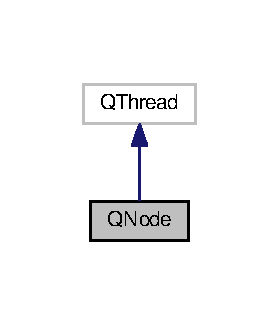
\includegraphics[width=134pt]{class_q_node__inherit__graph}
\end{center}
\end{figure}


Collaboration diagram for Q\+Node\+:
\nopagebreak
\begin{figure}[H]
\begin{center}
\leavevmode
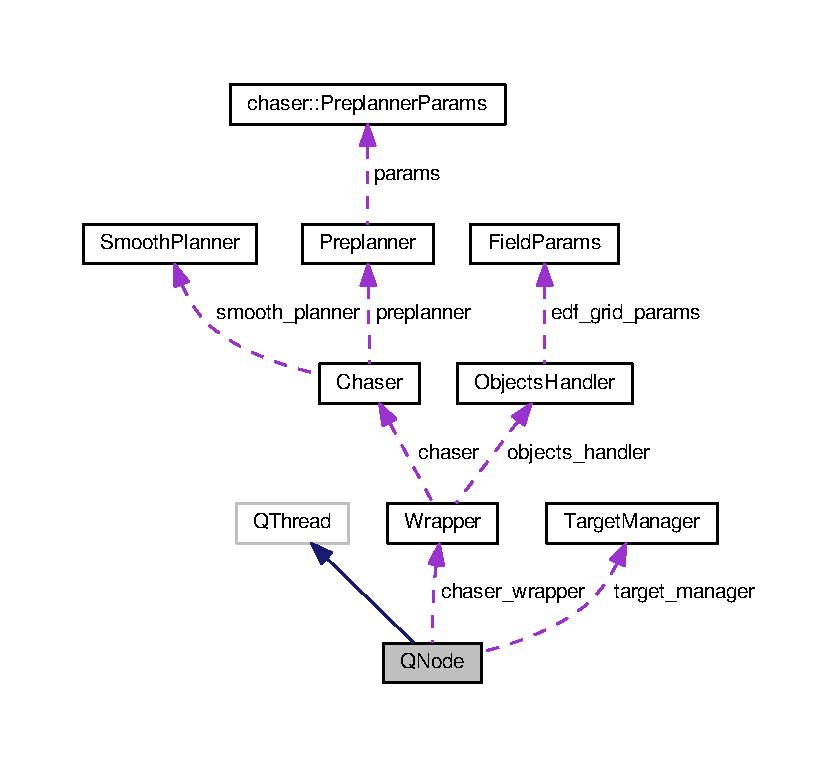
\includegraphics[width=350pt]{class_q_node__coll__graph}
\end{center}
\end{figure}
\subsection*{Signals}
\begin{DoxyCompactItemize}
\item 
void \hyperlink{class_q_node_abddcd4e0187f6d4513bbee7ba4656827}{logging\+Updated} ()
\item 
void \hyperlink{class_q_node_a7888b171c93c5f47334f5d2815adf445}{ros\+Shutdown} ()
\item 
void \hyperlink{class_q_node_a80d139522a1333db2c6ea33914c32378}{write\+On\+Board} (Q\+String)
\end{DoxyCompactItemize}
\subsection*{Public Member Functions}
\begin{DoxyCompactItemize}
\item 
\hyperlink{class_q_node_af26ee8c152283b4a1999dc5d4bd67908}{Q\+Node} (int argc, char $\ast$$\ast$argv, const std\+::string \&name)
\item 
\hyperlink{class_q_node_afed12669e9aed3e70721f507804778ca}{$\sim$\+Q\+Node} ()
\item 
bool \hyperlink{class_q_node_a32d00dbcf15c277e08caabf95af04f6e}{on\+\_\+init} ()
\item 
void \hyperlink{class_q_node_a770568addece696138f515d38408ff5c}{shutdown} ()
\item 
void \hyperlink{class_q_node_ae585b201389c51a177fa5e2fde252c84}{run} ()
\item 
bool \hyperlink{class_q_node_a65f0fc9f27f336150f33b53a7c51d80b}{trigger\+\_\+one\+\_\+shot} (double tf)
\item 
bool \hyperlink{class_q_node_a23bd7e0744ad4c7b5d5464485375bef1}{trigger} (double t\+\_\+cur)
\item 
Q\+String\+List\+Model $\ast$ \hyperlink{class_q_node_a0a6dae02f9e317488095367203fa8a58}{logging\+Model} ()
\item 
const std\+::string \& \hyperlink{class_q_node_ac21ae24311df97ac0e15c97179763b0e}{node\+Name} ()
\item 
void \hyperlink{class_q_node_a2b1b82bfd6e5e6187fe8216ba840bb09}{wpnts\+\_\+init} ()
\end{DoxyCompactItemize}
\subsection*{Public Attributes}
\begin{DoxyCompactItemize}
\item 
\hyperlink{class_target_manager}{Target\+Manager} \hyperlink{class_q_node_adc66765125dfd755d5e7f0c0eb6e6395}{target\+\_\+manager}
\item 
\hyperlink{class_wrapper}{Wrapper} \hyperlink{class_q_node_ad2d828488fb632a008c7d3ee0e1d1fa2}{chaser\+\_\+wrapper}
\item 
string \hyperlink{class_q_node_a0967d1922eeb7e39eedca309c7003d23}{write\+\_\+path}
\item 
bool \hyperlink{class_q_node_a98b08e7704b00df8648f8c08dffe950c}{is\+\_\+connected} = false
\item 
bool \hyperlink{class_q_node_a6ace2d0aa89adecfe699b3f1c3ce0b0f}{is\+\_\+in\+\_\+session} = false
\item 
bool \hyperlink{class_q_node_a9db73b60d8ffd6ac1e64ab5620f2db49}{is\+\_\+said\+\_\+edf} = false
\item 
double \hyperlink{class_q_node_a2893bbeba854c1cc89d2271804325b7b}{button\+\_\+elapsed} =0
\item 
double \hyperlink{class_q_node_ad1f3252201b932fc5d39b4f80349c7e2}{record\+\_\+dt} = 0.\+5
\item 
ros\+::\+Time \hyperlink{class_q_node_a96e6599c14732ded065ae6a5b004f872}{button\+\_\+click\+\_\+time}
\item 
double \hyperlink{class_q_node_a4b5f0a40821fbb176de620cb5a3921f7}{previous\+\_\+elapsed} = 0
\item 
double \hyperlink{class_q_node_a932e8eb11684f38ae2fb3f23639b7c70}{last\+\_\+tigger\+\_\+time} = 0
\item 
double \hyperlink{class_q_node_a7a127726e48aa5bde733d715af7a744c}{simulation\+\_\+end\+\_\+time}
\item 
double \hyperlink{class_q_node_a6e6b7e12d0d9bbc230cc9dc42a2bd087}{early\+\_\+end\+\_\+time} = 0.\+1
\item 
bool \hyperlink{class_q_node_ada91a6275708099206c452df47210045}{arrow\+\_\+record\+\_\+switch} = true
\item 
float \hyperlink{class_q_node_a3430f5db8c773c840b76794c82a9d58f}{pred\+\_\+horizon}
\item 
int \hyperlink{class_q_node_a5d5139bf1420415b2e0c2b0e52db957e}{prediction\+\_\+mode} = 0
\item 
int \hyperlink{class_q_node_aed4571afa880dc86a88b229c6517bfa1}{pred\+\_\+seq} = 4
\end{DoxyCompactItemize}
\subsection*{Protected Member Functions}
\begin{DoxyCompactItemize}
\item 
void \hyperlink{class_q_node_a498b0376fc75702fd8b61b91ef109769}{ros\+\_\+comms\+\_\+init} ()
\end{DoxyCompactItemize}
\subsection*{Protected Attributes}
\begin{DoxyCompactItemize}
\item 
int \hyperlink{class_q_node_aa0c7569195d8b9a6e568e98097f11d52}{init\+\_\+argc}
\item 
char $\ast$$\ast$ \hyperlink{class_q_node_a92c2972e3dd2a5de95d0edf8c75e1e5f}{init\+\_\+argv}
\item 
Q\+String\+List\+Model \hyperlink{class_q_node_aff2207dadd447d4c2554df19b6f7ce48}{logging}
\item 
const std\+::string \hyperlink{class_q_node_ae2a04cf101323be1e9b2be1e63a03b7f}{node\+\_\+name}
\end{DoxyCompactItemize}


\subsection{Detailed Description}


\subsection{Constructor \& Destructor Documentation}
\index{Q\+Node@{Q\+Node}!Q\+Node@{Q\+Node}}
\index{Q\+Node@{Q\+Node}!Q\+Node@{Q\+Node}}
\subsubsection[{\texorpdfstring{Q\+Node(int argc, char $\ast$$\ast$argv, const std\+::string \&name)}{QNode(int argc, char **argv, const std::string &name)}}]{\setlength{\rightskip}{0pt plus 5cm}Q\+Node\+::\+Q\+Node (
\begin{DoxyParamCaption}
\item[{int}]{argc, }
\item[{char $\ast$$\ast$}]{argv, }
\item[{const std\+::string \&}]{name}
\end{DoxyParamCaption}
)}\hypertarget{class_q_node_af26ee8c152283b4a1999dc5d4bd67908}{}\label{class_q_node_af26ee8c152283b4a1999dc5d4bd67908}

\begin{DoxyCode}
3                                                           :
4     \hyperlink{class_q_node_aa0c7569195d8b9a6e568e98097f11d52}{init\_argc}(argc),
5     \hyperlink{class_q_node_a92c2972e3dd2a5de95d0edf8c75e1e5f}{init\_argv}(argv),
6     \hyperlink{class_q_node_ae2a04cf101323be1e9b2be1e63a03b7f}{node\_name}(name)
7     \{
8         
9 \}
\end{DoxyCode}
\index{Q\+Node@{Q\+Node}!````~Q\+Node@{$\sim$\+Q\+Node}}
\index{````~Q\+Node@{$\sim$\+Q\+Node}!Q\+Node@{Q\+Node}}
\subsubsection[{\texorpdfstring{$\sim$\+Q\+Node()}{~QNode()}}]{\setlength{\rightskip}{0pt plus 5cm}Q\+Node\+::$\sim$\+Q\+Node (
\begin{DoxyParamCaption}
{}
\end{DoxyParamCaption}
)}\hypertarget{class_q_node_afed12669e9aed3e70721f507804778ca}{}\label{class_q_node_afed12669e9aed3e70721f507804778ca}

\begin{DoxyCode}
10 \{\}
\end{DoxyCode}


\subsection{Member Function Documentation}
\index{Q\+Node@{Q\+Node}!logging\+Model@{logging\+Model}}
\index{logging\+Model@{logging\+Model}!Q\+Node@{Q\+Node}}
\subsubsection[{\texorpdfstring{logging\+Model()}{loggingModel()}}]{\setlength{\rightskip}{0pt plus 5cm}Q\+String\+List\+Model$\ast$ Q\+Node\+::logging\+Model (
\begin{DoxyParamCaption}
{}
\end{DoxyParamCaption}
)\hspace{0.3cm}{\ttfamily [inline]}}\hypertarget{class_q_node_a0a6dae02f9e317488095367203fa8a58}{}\label{class_q_node_a0a6dae02f9e317488095367203fa8a58}

\begin{DoxyCode}
33 \{ \textcolor{keywordflow}{return} &\hyperlink{class_q_node_aff2207dadd447d4c2554df19b6f7ce48}{logging}; \}
\end{DoxyCode}
\index{Q\+Node@{Q\+Node}!logging\+Updated@{logging\+Updated}}
\index{logging\+Updated@{logging\+Updated}!Q\+Node@{Q\+Node}}
\subsubsection[{\texorpdfstring{logging\+Updated}{loggingUpdated}}]{\setlength{\rightskip}{0pt plus 5cm}void Q\+Node\+::logging\+Updated (
\begin{DoxyParamCaption}
{}
\end{DoxyParamCaption}
)\hspace{0.3cm}{\ttfamily [signal]}}\hypertarget{class_q_node_abddcd4e0187f6d4513bbee7ba4656827}{}\label{class_q_node_abddcd4e0187f6d4513bbee7ba4656827}
\index{Q\+Node@{Q\+Node}!node\+Name@{node\+Name}}
\index{node\+Name@{node\+Name}!Q\+Node@{Q\+Node}}
\subsubsection[{\texorpdfstring{node\+Name()}{nodeName()}}]{\setlength{\rightskip}{0pt plus 5cm}const std\+::string\& Q\+Node\+::node\+Name (
\begin{DoxyParamCaption}
{}
\end{DoxyParamCaption}
)\hspace{0.3cm}{\ttfamily [inline]}}\hypertarget{class_q_node_ac21ae24311df97ac0e15c97179763b0e}{}\label{class_q_node_ac21ae24311df97ac0e15c97179763b0e}

\begin{DoxyCode}
34 \{ \textcolor{keywordflow}{return} \hyperlink{class_q_node_ae2a04cf101323be1e9b2be1e63a03b7f}{node\_name}; \}
\end{DoxyCode}
\index{Q\+Node@{Q\+Node}!on\+\_\+init@{on\+\_\+init}}
\index{on\+\_\+init@{on\+\_\+init}!Q\+Node@{Q\+Node}}
\subsubsection[{\texorpdfstring{on\+\_\+init()}{on_init()}}]{\setlength{\rightskip}{0pt plus 5cm}bool Q\+Node\+::on\+\_\+init (
\begin{DoxyParamCaption}
{}
\end{DoxyParamCaption}
)}\hypertarget{class_q_node_a32d00dbcf15c277e08caabf95af04f6e}{}\label{class_q_node_a32d00dbcf15c277e08caabf95af04f6e}

\begin{DoxyCode}
34                    \{
35 
36     ros::init(\hyperlink{class_q_node_aa0c7569195d8b9a6e568e98097f11d52}{init\_argc},\hyperlink{class_q_node_a92c2972e3dd2a5de95d0edf8c75e1e5f}{init\_argv},\hyperlink{class_q_node_ae2a04cf101323be1e9b2be1e63a03b7f}{node\_name});
37     \textcolor{keywordflow}{if} ( ! ros::master::check() ) \{
38         \textcolor{keywordflow}{return} \textcolor{keyword}{false};
39     \}
40     ros::start(); \textcolor{comment}{// our node handles go out of scope, so we want to control shutdown explicitly.}
41     \hyperlink{class_q_node_a498b0376fc75702fd8b61b91ef109769}{ros\_comms\_init}();
42     start();
43     \textcolor{keywordflow}{return} \textcolor{keyword}{true};
44 \}
\end{DoxyCode}
\index{Q\+Node@{Q\+Node}!ros\+\_\+comms\+\_\+init@{ros\+\_\+comms\+\_\+init}}
\index{ros\+\_\+comms\+\_\+init@{ros\+\_\+comms\+\_\+init}!Q\+Node@{Q\+Node}}
\subsubsection[{\texorpdfstring{ros\+\_\+comms\+\_\+init()}{ros_comms_init()}}]{\setlength{\rightskip}{0pt plus 5cm}void Q\+Node\+::ros\+\_\+comms\+\_\+init (
\begin{DoxyParamCaption}
{}
\end{DoxyParamCaption}
)\hspace{0.3cm}{\ttfamily [protected]}}\hypertarget{class_q_node_a498b0376fc75702fd8b61b91ef109769}{}\label{class_q_node_a498b0376fc75702fd8b61b91ef109769}

\begin{DoxyCode}
11                           \{
12     
13     ros::NodeHandle nh(\textcolor{stringliteral}{"~"});
14     nh.param(\textcolor{stringliteral}{"pred\_horizon"},\hyperlink{class_q_node_a3430f5db8c773c840b76794c82a9d58f}{pred\_horizon},\textcolor{keywordtype}{float}(3.0));
15     nh.param(\textcolor{stringliteral}{"early\_end\_time"},\hyperlink{class_q_node_a6e6b7e12d0d9bbc230cc9dc42a2bd087}{early\_end\_time},0.1);
16     nh.param<\textcolor{keywordtype}{int}>(\textcolor{stringliteral}{"pred\_seq"},\hyperlink{class_q_node_aed4571afa880dc86a88b229c6517bfa1}{pred\_seq},4);
17 
18     \textcolor{comment}{// target manager init}
19     this->\hyperlink{class_q_node_adc66765125dfd755d5e7f0c0eb6e6395}{target\_manager}.\hyperlink{class_target_manager_a293bcb3b559c6e7c4ef549873791f092}{init}(nh);
20 
21     \textcolor{comment}{// wrapper init}
22     this->\hyperlink{class_q_node_ad2d828488fb632a008c7d3ee0e1d1fa2}{chaser\_wrapper}.\hyperlink{class_wrapper_af336781e7d75d525e7b152366a0e0d93}{init}(nh);
23 
24 \}
\end{DoxyCode}
\index{Q\+Node@{Q\+Node}!ros\+Shutdown@{ros\+Shutdown}}
\index{ros\+Shutdown@{ros\+Shutdown}!Q\+Node@{Q\+Node}}
\subsubsection[{\texorpdfstring{ros\+Shutdown}{rosShutdown}}]{\setlength{\rightskip}{0pt plus 5cm}void Q\+Node\+::ros\+Shutdown (
\begin{DoxyParamCaption}
{}
\end{DoxyParamCaption}
)\hspace{0.3cm}{\ttfamily [signal]}}\hypertarget{class_q_node_a7888b171c93c5f47334f5d2815adf445}{}\label{class_q_node_a7888b171c93c5f47334f5d2815adf445}
\index{Q\+Node@{Q\+Node}!run@{run}}
\index{run@{run}!Q\+Node@{Q\+Node}}
\subsubsection[{\texorpdfstring{run()}{run()}}]{\setlength{\rightskip}{0pt plus 5cm}void Q\+Node\+::run (
\begin{DoxyParamCaption}
{}
\end{DoxyParamCaption}
)}\hypertarget{class_q_node_ae585b201389c51a177fa5e2fde252c84}{}\label{class_q_node_ae585b201389c51a177fa5e2fde252c84}

\begin{DoxyCode}
46                \{
47     ros::Rate loop\_rate(50);
48     \hyperlink{class_q_node_a80d139522a1333db2c6ea33914c32378}{writeOnBoard}(\textcolor{stringliteral}{"waiting EDF computation..."});
49 
50     \textcolor{keywordflow}{while}(ros::ok())\{
51         \textcolor{keywordtype}{double} sim\_time;
52         
53         \textcolor{keywordflow}{if}(\hyperlink{class_q_node_a6ace2d0aa89adecfe699b3f1c3ce0b0f}{is\_in\_session})\{ \textcolor{comment}{// activated}
54             \textcolor{comment}{// current simulation time}
55             sim\_time = \hyperlink{class_q_node_a4b5f0a40821fbb176de620cb5a3921f7}{previous\_elapsed} + (ros::Time::now() - 
      \hyperlink{class_q_node_a96e6599c14732ded065ae6a5b004f872}{button\_click\_time}).toSec();
56             
57             \textcolor{comment}{// trigger condition }
58             \textcolor{keywordtype}{bool} trigger\_condition;
59             \textcolor{keywordflow}{if}(\hyperlink{class_q_node_a5d5139bf1420415b2e0c2b0e52db957e}{prediction\_mode} == 0)
60                 trigger\_condition = (\hyperlink{class_q_node_a932e8eb11684f38ae2fb3f23639b7c70}{last\_tigger\_time} == 0 or (sim\_time - 
      \hyperlink{class_q_node_a932e8eb11684f38ae2fb3f23639b7c70}{last\_tigger\_time}) > \hyperlink{class_q_node_a3430f5db8c773c840b76794c82a9d58f}{pred\_horizon} - \hyperlink{class_q_node_a6e6b7e12d0d9bbc230cc9dc42a2bd087}{early\_end\_time} ) and sim\_time 
      <\hyperlink{class_q_node_a7a127726e48aa5bde733d715af7a744c}{simulation\_end\_time};
61             \textcolor{keywordflow}{else} 
62                 trigger\_condition = \textcolor{keyword}{false}; \textcolor{comment}{// TODO for real prediction case }
63 
64             \textcolor{comment}{// if triggered do the followings }
65             \textcolor{keywordflow}{if}(trigger\_condition)                                
66                 \hyperlink{class_q_node_a23bd7e0744ad4c7b5d5464485375bef1}{trigger}(sim\_time);
67             
68        
69         \}\textcolor{keywordflow}{else}
70             sim\_time = \hyperlink{class_q_node_a4b5f0a40821fbb176de620cb5a3921f7}{previous\_elapsed}; 
71         
72         \textcolor{comment}{// session (publish the current information)        }
73         \hyperlink{class_q_node_adc66765125dfd755d5e7f0c0eb6e6395}{target\_manager}.\hyperlink{class_target_manager_a4af88c70bb8a0af0171ee9a49536d5c0}{session}(sim\_time);
74         \hyperlink{class_q_node_ad2d828488fb632a008c7d3ee0e1d1fa2}{chaser\_wrapper}.\hyperlink{class_wrapper_a009ee5c325926f92df42319d5469a376}{session}(sim\_time);
75         
76 
77         \textcolor{comment}{// chaser information board }
78         \textcolor{keywordflow}{if}(\hyperlink{class_q_node_ad2d828488fb632a008c7d3ee0e1d1fa2}{chaser\_wrapper}.\hyperlink{class_wrapper_a8cddd5ffbaeb5ab0b5d8d8d0c74f810f}{objects\_handler}.
      \hyperlink{class_objects_handler_acf1ef1b318defc2a39d87cea72689478}{is\_map\_recieved} and (not \hyperlink{class_q_node_a9db73b60d8ffd6ac1e64ab5620f2db49}{is\_said\_edf}))\{
79             \hyperlink{class_q_node_a80d139522a1333db2c6ea33914c32378}{writeOnBoard}(\textcolor{stringliteral}{"EDF loaded."});
80             is\_said\_edf = \textcolor{keyword}{true};
81         \}
82         
83         ros::spinOnce();
84         loop\_rate.sleep();
85     \}
86 
87 
88     Q\_EMIT \hyperlink{class_q_node_a7888b171c93c5f47334f5d2815adf445}{rosShutdown}();
89 
90 \}
\end{DoxyCode}
\index{Q\+Node@{Q\+Node}!shutdown@{shutdown}}
\index{shutdown@{shutdown}!Q\+Node@{Q\+Node}}
\subsubsection[{\texorpdfstring{shutdown()}{shutdown()}}]{\setlength{\rightskip}{0pt plus 5cm}void Q\+Node\+::shutdown (
\begin{DoxyParamCaption}
{}
\end{DoxyParamCaption}
)}\hypertarget{class_q_node_a770568addece696138f515d38408ff5c}{}\label{class_q_node_a770568addece696138f515d38408ff5c}

\begin{DoxyCode}
26                      \{
27     \textcolor{keywordflow}{if}(ros::isStarted()) \{
28       ros::shutdown(); \textcolor{comment}{// explicitly needed since we use ros::start();}
29       ros::waitForShutdown();
30     \}
31     wait();
32 \}
\end{DoxyCode}
\index{Q\+Node@{Q\+Node}!trigger@{trigger}}
\index{trigger@{trigger}!Q\+Node@{Q\+Node}}
\subsubsection[{\texorpdfstring{trigger(double t\+\_\+cur)}{trigger(double t_cur)}}]{\setlength{\rightskip}{0pt plus 5cm}bool Q\+Node\+::trigger (
\begin{DoxyParamCaption}
\item[{double}]{t\+\_\+cur}
\end{DoxyParamCaption}
)}\hypertarget{class_q_node_a23bd7e0744ad4c7b5d5464485375bef1}{}\label{class_q_node_a23bd7e0744ad4c7b5d5464485375bef1}

\begin{DoxyCode}
118                                \{
119 
120     \hyperlink{class_q_node_a932e8eb11684f38ae2fb3f23639b7c70}{last\_tigger\_time} = t\_cur;
121     VectorXd pred\_horizon\_vec(\hyperlink{class_q_node_aed4571afa880dc86a88b229c6517bfa1}{pred\_seq});
122     pred\_horizon\_vec.setLinSpaced(\hyperlink{class_q_node_aed4571afa880dc86a88b229c6517bfa1}{pred\_seq},t\_cur,t\_cur + \hyperlink{class_q_node_a3430f5db8c773c840b76794c82a9d58f}{pred\_horizon}); 
123     \textcolor{comment}{// if(t\_cur + pred\_horizon > simulation\_end\_time)\{}
124 
125     \textcolor{comment}{//     cout<<"almost there"<<endl;}
126     \textcolor{comment}{// \}}
127     \textcolor{comment}{// pred\_horizon\_vec = pred\_horizon\_vec.cwiseMin(simulation\_end\_time); // clamping with final time}
128     cout<<\textcolor{stringliteral}{"current horizon vector:\(\backslash\)n"}<<pred\_horizon\_vec<<endl; 
129     \textcolor{comment}{// we chase under this prediction }
130     vector<Point> target\_seq = \hyperlink{class_q_node_adc66765125dfd755d5e7f0c0eb6e6395}{target\_manager}.\hyperlink{class_target_manager_a63bbc724844890316a654380d0354e93}{eval\_time\_seq}(pred\_horizon\_vec);
131     
132     \textcolor{keywordflow}{if} (target\_seq.size() == 0)\{
133         this->\hyperlink{class_q_node_a80d139522a1333db2c6ea33914c32378}{writeOnBoard}(\textcolor{stringliteral}{"size of provided target sequence is zero. please generate target
       traj first."});
134         \textcolor{keywordflow}{return} \textcolor{keyword}{false};
135     \}
136     \textcolor{keywordflow}{if}(not \hyperlink{class_q_node_ad2d828488fb632a008c7d3ee0e1d1fa2}{chaser\_wrapper}.\hyperlink{class_wrapper_a8cddd5ffbaeb5ab0b5d8d8d0c74f810f}{objects\_handler}.
      \hyperlink{class_objects_handler_a16165ae7c0167ba8d2a0151a8a4fbfd5}{is\_chaser\_spawned})\{
137         this->\hyperlink{class_q_node_a80d139522a1333db2c6ea33914c32378}{writeOnBoard}(\textcolor{stringliteral}{"chaser has not been spawned."});
138         \textcolor{keywordflow}{return} \textcolor{keyword}{false};
139     \}
140 
141     \textcolor{keywordflow}{if}(not \hyperlink{class_q_node_ad2d828488fb632a008c7d3ee0e1d1fa2}{chaser\_wrapper}.\hyperlink{class_wrapper_a8cddd5ffbaeb5ab0b5d8d8d0c74f810f}{objects\_handler}.
      \hyperlink{class_objects_handler_acf1ef1b318defc2a39d87cea72689478}{is\_map\_recieved})\{
142         this->\hyperlink{class_q_node_a80d139522a1333db2c6ea33914c32378}{writeOnBoard}(\textcolor{stringliteral}{"octomap or edf has not been uploaded."});
143         \textcolor{keywordflow}{return} \textcolor{keyword}{false};
144     \}    
145 
146 
147     \textcolor{keywordflow}{return} \hyperlink{class_q_node_ad2d828488fb632a008c7d3ee0e1d1fa2}{chaser\_wrapper}.\hyperlink{class_wrapper_a21a0e115ea80e053e4f2defd1362b92f}{trigger\_chasing}(target\_seq,pred\_horizon\_vec); 
148 \}\end{DoxyCode}
\index{Q\+Node@{Q\+Node}!trigger\+\_\+one\+\_\+shot@{trigger\+\_\+one\+\_\+shot}}
\index{trigger\+\_\+one\+\_\+shot@{trigger\+\_\+one\+\_\+shot}!Q\+Node@{Q\+Node}}
\subsubsection[{\texorpdfstring{trigger\+\_\+one\+\_\+shot(double tf)}{trigger_one_shot(double tf)}}]{\setlength{\rightskip}{0pt plus 5cm}bool Q\+Node\+::trigger\+\_\+one\+\_\+shot (
\begin{DoxyParamCaption}
\item[{double}]{tf}
\end{DoxyParamCaption}
)}\hypertarget{class_q_node_a65f0fc9f27f336150f33b53a7c51d80b}{}\label{class_q_node_a65f0fc9f27f336150f33b53a7c51d80b}

\begin{DoxyCode}
92                                      \{
93     
94 
95 
96     \textcolor{comment}{// target global waypoitns  }
97     vector<Point> target\_seq = \hyperlink{_common_8h_a81915b091c29bc9aef6a74ab374f479a}{extract\_pnts\_from\_path}(
      \hyperlink{class_q_node_adc66765125dfd755d5e7f0c0eb6e6395}{target\_manager}.\hyperlink{class_target_manager_a747b82bf5cb4d1d3574dbc08a117538f}{get\_global\_waypoints}());
98     \textcolor{keywordflow}{if} (target\_seq.size() == 0)\{
99         this->\hyperlink{class_q_node_a80d139522a1333db2c6ea33914c32378}{writeOnBoard}(\textcolor{stringliteral}{"size of provided target sequence is zero. please generate target
       traj first."});
100         \textcolor{keywordflow}{return} \textcolor{keyword}{false};
101     \}
102     \textcolor{keywordflow}{if}(not \hyperlink{class_q_node_ad2d828488fb632a008c7d3ee0e1d1fa2}{chaser\_wrapper}.\hyperlink{class_wrapper_a8cddd5ffbaeb5ab0b5d8d8d0c74f810f}{objects\_handler}.
      \hyperlink{class_objects_handler_a16165ae7c0167ba8d2a0151a8a4fbfd5}{is\_chaser\_spawned})\{
103         this->\hyperlink{class_q_node_a80d139522a1333db2c6ea33914c32378}{writeOnBoard}(\textcolor{stringliteral}{"chaser has not been spawned."});
104         \textcolor{keywordflow}{return} \textcolor{keyword}{false};
105     \}
106 
107     \textcolor{keywordflow}{if}(not \hyperlink{class_q_node_ad2d828488fb632a008c7d3ee0e1d1fa2}{chaser\_wrapper}.\hyperlink{class_wrapper_a8cddd5ffbaeb5ab0b5d8d8d0c74f810f}{objects\_handler}.
      \hyperlink{class_objects_handler_acf1ef1b318defc2a39d87cea72689478}{is\_map\_recieved})\{
108         this->\hyperlink{class_q_node_a80d139522a1333db2c6ea33914c32378}{writeOnBoard}(\textcolor{stringliteral}{"octomap or edf has not been uploaded."});
109         \textcolor{keywordflow}{return} \textcolor{keyword}{false};
110     \}    
111 
112     \textcolor{comment}{// trigger chasing}
113     VectorXd knots;    
114     knots.setLinSpaced(\hyperlink{class_q_node_adc66765125dfd755d5e7f0c0eb6e6395}{target\_manager}.\hyperlink{class_target_manager_a0bbcb1981504e3bc587c3a98f41a91e9}{queue}.size(),0,tf); 
115     \textcolor{keywordtype}{bool} is\_success =  \hyperlink{class_q_node_ad2d828488fb632a008c7d3ee0e1d1fa2}{chaser\_wrapper}.\hyperlink{class_wrapper_a21a0e115ea80e053e4f2defd1362b92f}{trigger\_chasing}(target\_seq,knots);      
        
116 \}
\end{DoxyCode}
\index{Q\+Node@{Q\+Node}!wpnts\+\_\+init@{wpnts\+\_\+init}}
\index{wpnts\+\_\+init@{wpnts\+\_\+init}!Q\+Node@{Q\+Node}}
\subsubsection[{\texorpdfstring{wpnts\+\_\+init()}{wpnts_init()}}]{\setlength{\rightskip}{0pt plus 5cm}void Q\+Node\+::wpnts\+\_\+init (
\begin{DoxyParamCaption}
{}
\end{DoxyParamCaption}
)}\hypertarget{class_q_node_a2b1b82bfd6e5e6187fe8216ba840bb09}{}\label{class_q_node_a2b1b82bfd6e5e6187fe8216ba840bb09}
\index{Q\+Node@{Q\+Node}!write\+On\+Board@{write\+On\+Board}}
\index{write\+On\+Board@{write\+On\+Board}!Q\+Node@{Q\+Node}}
\subsubsection[{\texorpdfstring{write\+On\+Board}{writeOnBoard}}]{\setlength{\rightskip}{0pt plus 5cm}void Q\+Node\+::write\+On\+Board (
\begin{DoxyParamCaption}
\item[{Q\+String}]{}
\end{DoxyParamCaption}
)\hspace{0.3cm}{\ttfamily [signal]}}\hypertarget{class_q_node_a80d139522a1333db2c6ea33914c32378}{}\label{class_q_node_a80d139522a1333db2c6ea33914c32378}


\subsection{Member Data Documentation}
\index{Q\+Node@{Q\+Node}!arrow\+\_\+record\+\_\+switch@{arrow\+\_\+record\+\_\+switch}}
\index{arrow\+\_\+record\+\_\+switch@{arrow\+\_\+record\+\_\+switch}!Q\+Node@{Q\+Node}}
\subsubsection[{\texorpdfstring{arrow\+\_\+record\+\_\+switch}{arrow_record_switch}}]{\setlength{\rightskip}{0pt plus 5cm}bool Q\+Node\+::arrow\+\_\+record\+\_\+switch = true}\hypertarget{class_q_node_ada91a6275708099206c452df47210045}{}\label{class_q_node_ada91a6275708099206c452df47210045}
\index{Q\+Node@{Q\+Node}!button\+\_\+click\+\_\+time@{button\+\_\+click\+\_\+time}}
\index{button\+\_\+click\+\_\+time@{button\+\_\+click\+\_\+time}!Q\+Node@{Q\+Node}}
\subsubsection[{\texorpdfstring{button\+\_\+click\+\_\+time}{button_click_time}}]{\setlength{\rightskip}{0pt plus 5cm}ros\+::\+Time Q\+Node\+::button\+\_\+click\+\_\+time}\hypertarget{class_q_node_a96e6599c14732ded065ae6a5b004f872}{}\label{class_q_node_a96e6599c14732ded065ae6a5b004f872}
\index{Q\+Node@{Q\+Node}!button\+\_\+elapsed@{button\+\_\+elapsed}}
\index{button\+\_\+elapsed@{button\+\_\+elapsed}!Q\+Node@{Q\+Node}}
\subsubsection[{\texorpdfstring{button\+\_\+elapsed}{button_elapsed}}]{\setlength{\rightskip}{0pt plus 5cm}double Q\+Node\+::button\+\_\+elapsed =0}\hypertarget{class_q_node_a2893bbeba854c1cc89d2271804325b7b}{}\label{class_q_node_a2893bbeba854c1cc89d2271804325b7b}
\index{Q\+Node@{Q\+Node}!chaser\+\_\+wrapper@{chaser\+\_\+wrapper}}
\index{chaser\+\_\+wrapper@{chaser\+\_\+wrapper}!Q\+Node@{Q\+Node}}
\subsubsection[{\texorpdfstring{chaser\+\_\+wrapper}{chaser_wrapper}}]{\setlength{\rightskip}{0pt plus 5cm}{\bf Wrapper} Q\+Node\+::chaser\+\_\+wrapper}\hypertarget{class_q_node_ad2d828488fb632a008c7d3ee0e1d1fa2}{}\label{class_q_node_ad2d828488fb632a008c7d3ee0e1d1fa2}
\index{Q\+Node@{Q\+Node}!early\+\_\+end\+\_\+time@{early\+\_\+end\+\_\+time}}
\index{early\+\_\+end\+\_\+time@{early\+\_\+end\+\_\+time}!Q\+Node@{Q\+Node}}
\subsubsection[{\texorpdfstring{early\+\_\+end\+\_\+time}{early_end_time}}]{\setlength{\rightskip}{0pt plus 5cm}double Q\+Node\+::early\+\_\+end\+\_\+time = 0.\+1}\hypertarget{class_q_node_a6e6b7e12d0d9bbc230cc9dc42a2bd087}{}\label{class_q_node_a6e6b7e12d0d9bbc230cc9dc42a2bd087}
\index{Q\+Node@{Q\+Node}!init\+\_\+argc@{init\+\_\+argc}}
\index{init\+\_\+argc@{init\+\_\+argc}!Q\+Node@{Q\+Node}}
\subsubsection[{\texorpdfstring{init\+\_\+argc}{init_argc}}]{\setlength{\rightskip}{0pt plus 5cm}int Q\+Node\+::init\+\_\+argc\hspace{0.3cm}{\ttfamily [protected]}}\hypertarget{class_q_node_aa0c7569195d8b9a6e568e98097f11d52}{}\label{class_q_node_aa0c7569195d8b9a6e568e98097f11d52}
\index{Q\+Node@{Q\+Node}!init\+\_\+argv@{init\+\_\+argv}}
\index{init\+\_\+argv@{init\+\_\+argv}!Q\+Node@{Q\+Node}}
\subsubsection[{\texorpdfstring{init\+\_\+argv}{init_argv}}]{\setlength{\rightskip}{0pt plus 5cm}char$\ast$$\ast$ Q\+Node\+::init\+\_\+argv\hspace{0.3cm}{\ttfamily [protected]}}\hypertarget{class_q_node_a92c2972e3dd2a5de95d0edf8c75e1e5f}{}\label{class_q_node_a92c2972e3dd2a5de95d0edf8c75e1e5f}
\index{Q\+Node@{Q\+Node}!is\+\_\+connected@{is\+\_\+connected}}
\index{is\+\_\+connected@{is\+\_\+connected}!Q\+Node@{Q\+Node}}
\subsubsection[{\texorpdfstring{is\+\_\+connected}{is_connected}}]{\setlength{\rightskip}{0pt plus 5cm}bool Q\+Node\+::is\+\_\+connected = false}\hypertarget{class_q_node_a98b08e7704b00df8648f8c08dffe950c}{}\label{class_q_node_a98b08e7704b00df8648f8c08dffe950c}
\index{Q\+Node@{Q\+Node}!is\+\_\+in\+\_\+session@{is\+\_\+in\+\_\+session}}
\index{is\+\_\+in\+\_\+session@{is\+\_\+in\+\_\+session}!Q\+Node@{Q\+Node}}
\subsubsection[{\texorpdfstring{is\+\_\+in\+\_\+session}{is_in_session}}]{\setlength{\rightskip}{0pt plus 5cm}bool Q\+Node\+::is\+\_\+in\+\_\+session = false}\hypertarget{class_q_node_a6ace2d0aa89adecfe699b3f1c3ce0b0f}{}\label{class_q_node_a6ace2d0aa89adecfe699b3f1c3ce0b0f}
\index{Q\+Node@{Q\+Node}!is\+\_\+said\+\_\+edf@{is\+\_\+said\+\_\+edf}}
\index{is\+\_\+said\+\_\+edf@{is\+\_\+said\+\_\+edf}!Q\+Node@{Q\+Node}}
\subsubsection[{\texorpdfstring{is\+\_\+said\+\_\+edf}{is_said_edf}}]{\setlength{\rightskip}{0pt plus 5cm}bool Q\+Node\+::is\+\_\+said\+\_\+edf = false}\hypertarget{class_q_node_a9db73b60d8ffd6ac1e64ab5620f2db49}{}\label{class_q_node_a9db73b60d8ffd6ac1e64ab5620f2db49}
\index{Q\+Node@{Q\+Node}!last\+\_\+tigger\+\_\+time@{last\+\_\+tigger\+\_\+time}}
\index{last\+\_\+tigger\+\_\+time@{last\+\_\+tigger\+\_\+time}!Q\+Node@{Q\+Node}}
\subsubsection[{\texorpdfstring{last\+\_\+tigger\+\_\+time}{last_tigger_time}}]{\setlength{\rightskip}{0pt plus 5cm}double Q\+Node\+::last\+\_\+tigger\+\_\+time = 0}\hypertarget{class_q_node_a932e8eb11684f38ae2fb3f23639b7c70}{}\label{class_q_node_a932e8eb11684f38ae2fb3f23639b7c70}
\index{Q\+Node@{Q\+Node}!logging@{logging}}
\index{logging@{logging}!Q\+Node@{Q\+Node}}
\subsubsection[{\texorpdfstring{logging}{logging}}]{\setlength{\rightskip}{0pt plus 5cm}Q\+String\+List\+Model Q\+Node\+::logging\hspace{0.3cm}{\ttfamily [protected]}}\hypertarget{class_q_node_aff2207dadd447d4c2554df19b6f7ce48}{}\label{class_q_node_aff2207dadd447d4c2554df19b6f7ce48}
\index{Q\+Node@{Q\+Node}!node\+\_\+name@{node\+\_\+name}}
\index{node\+\_\+name@{node\+\_\+name}!Q\+Node@{Q\+Node}}
\subsubsection[{\texorpdfstring{node\+\_\+name}{node_name}}]{\setlength{\rightskip}{0pt plus 5cm}const std\+::string Q\+Node\+::node\+\_\+name\hspace{0.3cm}{\ttfamily [protected]}}\hypertarget{class_q_node_ae2a04cf101323be1e9b2be1e63a03b7f}{}\label{class_q_node_ae2a04cf101323be1e9b2be1e63a03b7f}
\index{Q\+Node@{Q\+Node}!pred\+\_\+horizon@{pred\+\_\+horizon}}
\index{pred\+\_\+horizon@{pred\+\_\+horizon}!Q\+Node@{Q\+Node}}
\subsubsection[{\texorpdfstring{pred\+\_\+horizon}{pred_horizon}}]{\setlength{\rightskip}{0pt plus 5cm}float Q\+Node\+::pred\+\_\+horizon}\hypertarget{class_q_node_a3430f5db8c773c840b76794c82a9d58f}{}\label{class_q_node_a3430f5db8c773c840b76794c82a9d58f}
\index{Q\+Node@{Q\+Node}!pred\+\_\+seq@{pred\+\_\+seq}}
\index{pred\+\_\+seq@{pred\+\_\+seq}!Q\+Node@{Q\+Node}}
\subsubsection[{\texorpdfstring{pred\+\_\+seq}{pred_seq}}]{\setlength{\rightskip}{0pt plus 5cm}int Q\+Node\+::pred\+\_\+seq = 4}\hypertarget{class_q_node_aed4571afa880dc86a88b229c6517bfa1}{}\label{class_q_node_aed4571afa880dc86a88b229c6517bfa1}
\index{Q\+Node@{Q\+Node}!prediction\+\_\+mode@{prediction\+\_\+mode}}
\index{prediction\+\_\+mode@{prediction\+\_\+mode}!Q\+Node@{Q\+Node}}
\subsubsection[{\texorpdfstring{prediction\+\_\+mode}{prediction_mode}}]{\setlength{\rightskip}{0pt plus 5cm}int Q\+Node\+::prediction\+\_\+mode = 0}\hypertarget{class_q_node_a5d5139bf1420415b2e0c2b0e52db957e}{}\label{class_q_node_a5d5139bf1420415b2e0c2b0e52db957e}
\index{Q\+Node@{Q\+Node}!previous\+\_\+elapsed@{previous\+\_\+elapsed}}
\index{previous\+\_\+elapsed@{previous\+\_\+elapsed}!Q\+Node@{Q\+Node}}
\subsubsection[{\texorpdfstring{previous\+\_\+elapsed}{previous_elapsed}}]{\setlength{\rightskip}{0pt plus 5cm}double Q\+Node\+::previous\+\_\+elapsed = 0}\hypertarget{class_q_node_a4b5f0a40821fbb176de620cb5a3921f7}{}\label{class_q_node_a4b5f0a40821fbb176de620cb5a3921f7}
\index{Q\+Node@{Q\+Node}!record\+\_\+dt@{record\+\_\+dt}}
\index{record\+\_\+dt@{record\+\_\+dt}!Q\+Node@{Q\+Node}}
\subsubsection[{\texorpdfstring{record\+\_\+dt}{record_dt}}]{\setlength{\rightskip}{0pt plus 5cm}double Q\+Node\+::record\+\_\+dt = 0.\+5}\hypertarget{class_q_node_ad1f3252201b932fc5d39b4f80349c7e2}{}\label{class_q_node_ad1f3252201b932fc5d39b4f80349c7e2}
\index{Q\+Node@{Q\+Node}!simulation\+\_\+end\+\_\+time@{simulation\+\_\+end\+\_\+time}}
\index{simulation\+\_\+end\+\_\+time@{simulation\+\_\+end\+\_\+time}!Q\+Node@{Q\+Node}}
\subsubsection[{\texorpdfstring{simulation\+\_\+end\+\_\+time}{simulation_end_time}}]{\setlength{\rightskip}{0pt plus 5cm}double Q\+Node\+::simulation\+\_\+end\+\_\+time}\hypertarget{class_q_node_a7a127726e48aa5bde733d715af7a744c}{}\label{class_q_node_a7a127726e48aa5bde733d715af7a744c}
\index{Q\+Node@{Q\+Node}!target\+\_\+manager@{target\+\_\+manager}}
\index{target\+\_\+manager@{target\+\_\+manager}!Q\+Node@{Q\+Node}}
\subsubsection[{\texorpdfstring{target\+\_\+manager}{target_manager}}]{\setlength{\rightskip}{0pt plus 5cm}{\bf Target\+Manager} Q\+Node\+::target\+\_\+manager}\hypertarget{class_q_node_adc66765125dfd755d5e7f0c0eb6e6395}{}\label{class_q_node_adc66765125dfd755d5e7f0c0eb6e6395}
\index{Q\+Node@{Q\+Node}!write\+\_\+path@{write\+\_\+path}}
\index{write\+\_\+path@{write\+\_\+path}!Q\+Node@{Q\+Node}}
\subsubsection[{\texorpdfstring{write\+\_\+path}{write_path}}]{\setlength{\rightskip}{0pt plus 5cm}string Q\+Node\+::write\+\_\+path}\hypertarget{class_q_node_a0967d1922eeb7e39eedca309c7003d23}{}\label{class_q_node_a0967d1922eeb7e39eedca309c7003d23}


The documentation for this class was generated from the following files\+:\begin{DoxyCompactItemize}
\item 
src/qt\+\_\+ui/\hyperlink{qnode_8h}{qnode.\+h}\item 
src/qt\+\_\+ui/\hyperlink{qnode_8cpp}{qnode.\+cpp}\end{DoxyCompactItemize}

\hypertarget{class_smooth_planner}{}\section{Smooth\+Planner Class Reference}
\label{class_smooth_planner}\index{Smooth\+Planner@{Smooth\+Planner}}


{\ttfamily \#include $<$Smooth\+Planner.\+h$>$}

\subsection*{Public Member Functions}
\begin{DoxyCompactItemize}
\item 
\hyperlink{class_smooth_planner_a84977f10ce3e96fac997076324ca2909}{Smooth\+Planner} ()
\item 
void \hyperlink{class_smooth_planner_a34508c873d458075880afbae0e9c933e}{init} (ros\+::\+Node\+Handle nh)
\item 
void \hyperlink{class_smooth_planner_afc03abbd5f6473f2bc952f70195326ac}{traj\+\_\+gen} (Time\+Series knots, nav\+\_\+msgs\+::\+Path waypoints, Twist v0, Twist a0)
\item 
void \hyperlink{class_smooth_planner_a2996c73522e93adff70eb68e18c55951}{publish} ()
\end{DoxyCompactItemize}
\subsection*{Public Attributes}
\begin{DoxyCompactItemize}
\item 
Path\+Planner \hyperlink{class_smooth_planner_aa9df69d4f514c7338ab2d066d38dd1a2}{planner}
\item 
Traj\+Gen\+Opts \hyperlink{class_smooth_planner_af0c954aea3c6b5b82a160ed4be93fb17}{option}
\item 
ros\+::\+Publisher \hyperlink{class_smooth_planner_a7b8400f711456291e567d0fc204c274b}{pub\+\_\+path}
\item 
ros\+::\+Publisher \hyperlink{class_smooth_planner_a7cd9de34963f445a21a6d0101346b071}{pub\+\_\+chasing\+\_\+corridor}
\item 
ros\+::\+Publisher \hyperlink{class_smooth_planner_a7ee67bceac6d60409542a2250b2ccd08}{pub\+\_\+knots}
\item 
string \hyperlink{class_smooth_planner_ade278c4209b962d8342a2ee30e718c8b}{world\+\_\+frame\+\_\+id}
\item 
visualization\+\_\+msgs\+::\+Marker \hyperlink{class_smooth_planner_addf7aab458c1407f23e3544bd76ac82b}{chasing\+\_\+corridor}
\item 
nav\+\_\+msgs\+::\+Path \hyperlink{class_smooth_planner_a6a33038c6041ff972bea7765780b56d0}{chasing\+\_\+smooth\+\_\+path}
\item 
visualization\+\_\+msgs\+::\+Marker \hyperlink{class_smooth_planner_afeeab9ce830d4960babdc84c82da94ea}{marker\+\_\+knots}
\end{DoxyCompactItemize}


\subsection{Detailed Description}


\subsection{Constructor \& Destructor Documentation}
\index{Smooth\+Planner@{Smooth\+Planner}!Smooth\+Planner@{Smooth\+Planner}}
\index{Smooth\+Planner@{Smooth\+Planner}!Smooth\+Planner@{Smooth\+Planner}}
\subsubsection[{\texorpdfstring{Smooth\+Planner()}{SmoothPlanner()}}]{\setlength{\rightskip}{0pt plus 5cm}Smooth\+Planner\+::\+Smooth\+Planner (
\begin{DoxyParamCaption}
{}
\end{DoxyParamCaption}
)}\hypertarget{class_smooth_planner_a84977f10ce3e96fac997076324ca2909}{}\label{class_smooth_planner_a84977f10ce3e96fac997076324ca2909}

\begin{DoxyCode}
3 \{\}
\end{DoxyCode}


\subsection{Member Function Documentation}
\index{Smooth\+Planner@{Smooth\+Planner}!init@{init}}
\index{init@{init}!Smooth\+Planner@{Smooth\+Planner}}
\subsubsection[{\texorpdfstring{init(ros\+::\+Node\+Handle nh)}{init(ros::NodeHandle nh)}}]{\setlength{\rightskip}{0pt plus 5cm}void Smooth\+Planner\+::init (
\begin{DoxyParamCaption}
\item[{ros\+::\+Node\+Handle}]{nh}
\end{DoxyParamCaption}
)}\hypertarget{class_smooth_planner_a34508c873d458075880afbae0e9c933e}{}\label{class_smooth_planner_a34508c873d458075880afbae0e9c933e}

\begin{DoxyCode}
5                                         \{
6 
7     \textcolor{comment}{// paramter parsing for option }
8     nh.param<\textcolor{keywordtype}{string}>(\textcolor{stringliteral}{"world\_frame\_id"},\hyperlink{class_smooth_planner_ade278c4209b962d8342a2ee30e718c8b}{world\_frame\_id},\textcolor{stringliteral}{"/world"});
9     nh.param<\textcolor{keywordtype}{double}>(\textcolor{stringliteral}{"chaser/safe\_corridor\_r"},\hyperlink{class_smooth_planner_af0c954aea3c6b5b82a160ed4be93fb17}{option}.safe\_r,0.5);
10     nh.param<\textcolor{keywordtype}{int}>(\textcolor{stringliteral}{"chaser/N\_safe\_pnts"},\hyperlink{class_smooth_planner_af0c954aea3c6b5b82a160ed4be93fb17}{option}.N\_safe\_pnts,3);
11     nh.param<\textcolor{keywordtype}{int}>(\textcolor{stringliteral}{"chaser/objective\_derivative"},\hyperlink{class_smooth_planner_af0c954aea3c6b5b82a160ed4be93fb17}{option}.objective\_derivative,3);
12     nh.param<\textcolor{keywordtype}{bool}>(\textcolor{stringliteral}{"chaser/is\_multi\_corridor"},\hyperlink{class_smooth_planner_af0c954aea3c6b5b82a160ed4be93fb17}{option}.is\_multi\_corridor,\textcolor{keyword}{true});
13     nh.param<\textcolor{keywordtype}{bool}>(\textcolor{stringliteral}{"chaser/is\_waypoint\_soft"},\hyperlink{class_smooth_planner_af0c954aea3c6b5b82a160ed4be93fb17}{option}.is\_waypoint\_soft,\textcolor{keyword}{true});
14     nh.param<\textcolor{keywordtype}{double}>(\textcolor{stringliteral}{"chaser/w\_deviation"},\hyperlink{class_smooth_planner_af0c954aea3c6b5b82a160ed4be93fb17}{option}.w\_d,0.5);
15     nh.param<\textcolor{keywordtype}{int}>(\textcolor{stringliteral}{"chaser/poly\_order"},\hyperlink{class_smooth_planner_af0c954aea3c6b5b82a160ed4be93fb17}{option}.poly\_order,6);
16     nh.param<\textcolor{keywordtype}{bool}>(\textcolor{stringliteral}{"chaser/verbose"},\hyperlink{class_smooth_planner_af0c954aea3c6b5b82a160ed4be93fb17}{option}.verbose,\textcolor{keyword}{true});
17 
18     \hyperlink{class_smooth_planner_a7cd9de34963f445a21a6d0101346b071}{pub\_chasing\_corridor} = nh.advertise<visualization\_msgs::Marker>(\textcolor{stringliteral}{"chasing\_corridor"},
      1); 
19     \hyperlink{class_smooth_planner_a7b8400f711456291e567d0fc204c274b}{pub\_path} = nh.advertise<nav\_msgs::Path>(\textcolor{stringliteral}{"smooth\_path"},1);
20     \hyperlink{class_smooth_planner_a7ee67bceac6d60409542a2250b2ccd08}{pub\_knots} = nh.advertise<visualization\_msgs::Marker>(\textcolor{stringliteral}{"smooth\_path\_knots"},1);
21 
22     \hyperlink{class_smooth_planner_addf7aab458c1407f23e3544bd76ac82b}{chasing\_corridor}.header.frame\_id = \hyperlink{class_smooth_planner_ade278c4209b962d8342a2ee30e718c8b}{world\_frame\_id};
23     \hyperlink{class_smooth_planner_a6a33038c6041ff972bea7765780b56d0}{chasing\_smooth\_path}.header.frame\_id = \hyperlink{class_smooth_planner_ade278c4209b962d8342a2ee30e718c8b}{world\_frame\_id};
24 
25 \};
\end{DoxyCode}
\index{Smooth\+Planner@{Smooth\+Planner}!publish@{publish}}
\index{publish@{publish}!Smooth\+Planner@{Smooth\+Planner}}
\subsubsection[{\texorpdfstring{publish()}{publish()}}]{\setlength{\rightskip}{0pt plus 5cm}void Smooth\+Planner\+::publish (
\begin{DoxyParamCaption}
{}
\end{DoxyParamCaption}
)}\hypertarget{class_smooth_planner_a2996c73522e93adff70eb68e18c55951}{}\label{class_smooth_planner_a2996c73522e93adff70eb68e18c55951}

\begin{DoxyCode}
44                            \{
45     \hyperlink{class_smooth_planner_a7b8400f711456291e567d0fc204c274b}{pub\_path}.publish(\hyperlink{class_smooth_planner_a6a33038c6041ff972bea7765780b56d0}{chasing\_smooth\_path});
46     \hyperlink{class_smooth_planner_a7cd9de34963f445a21a6d0101346b071}{pub\_chasing\_corridor}.publish(\hyperlink{class_smooth_planner_addf7aab458c1407f23e3544bd76ac82b}{chasing\_corridor});    
47     \hyperlink{class_smooth_planner_a7ee67bceac6d60409542a2250b2ccd08}{pub\_knots}.publish(\hyperlink{class_smooth_planner_afeeab9ce830d4960babdc84c82da94ea}{marker\_knots});
48 \}\end{DoxyCode}
\index{Smooth\+Planner@{Smooth\+Planner}!traj\+\_\+gen@{traj\+\_\+gen}}
\index{traj\+\_\+gen@{traj\+\_\+gen}!Smooth\+Planner@{Smooth\+Planner}}
\subsubsection[{\texorpdfstring{traj\+\_\+gen(\+Time\+Series knots, nav\+\_\+msgs\+::\+Path waypoints, Twist v0, Twist a0)}{traj_gen(TimeSeries knots, nav_msgs::Path waypoints, Twist v0, Twist a0)}}]{\setlength{\rightskip}{0pt plus 5cm}void Smooth\+Planner\+::traj\+\_\+gen (
\begin{DoxyParamCaption}
\item[{Time\+Series}]{knots, }
\item[{nav\+\_\+msgs\+::\+Path}]{waypoints, }
\item[{Twist}]{v0, }
\item[{Twist}]{a0}
\end{DoxyParamCaption}
)}\hypertarget{class_smooth_planner_afc03abbd5f6473f2bc952f70195326ac}{}\label{class_smooth_planner_afc03abbd5f6473f2bc952f70195326ac}

\begin{DoxyCode}
28                                                                                      \{
29 
30     \hyperlink{class_smooth_planner_aa9df69d4f514c7338ab2d066d38dd1a2}{planner}.path\_gen(knots,waypoints,v0,a0,\hyperlink{class_smooth_planner_af0c954aea3c6b5b82a160ed4be93fb17}{option});
31     
32     \textcolor{keywordflow}{if} (\hyperlink{class_smooth_planner_aa9df69d4f514c7338ab2d066d38dd1a2}{planner}.is\_spline\_valid())\{
33         \textcolor{comment}{// markers update }
34         \hyperlink{class_smooth_planner_addf7aab458c1407f23e3544bd76ac82b}{chasing\_corridor} = \hyperlink{class_smooth_planner_aa9df69d4f514c7338ab2d066d38dd1a2}{planner}.get\_safe\_corridor\_marker();
35         \hyperlink{class_smooth_planner_addf7aab458c1407f23e3544bd76ac82b}{chasing\_corridor}.header.frame\_id = \hyperlink{class_smooth_planner_ade278c4209b962d8342a2ee30e718c8b}{world\_frame\_id};
36         \hyperlink{class_smooth_planner_a6a33038c6041ff972bea7765780b56d0}{chasing\_smooth\_path} = \hyperlink{class_smooth_planner_aa9df69d4f514c7338ab2d066d38dd1a2}{planner}.get\_path();
37         \hyperlink{class_smooth_planner_a6a33038c6041ff972bea7765780b56d0}{chasing\_smooth\_path}.header.frame\_id = \hyperlink{class_smooth_planner_ade278c4209b962d8342a2ee30e718c8b}{world\_frame\_id};        
38         \hyperlink{class_smooth_planner_afeeab9ce830d4960babdc84c82da94ea}{marker\_knots} = \hyperlink{class_smooth_planner_aa9df69d4f514c7338ab2d066d38dd1a2}{planner}.get\_knots\_marker();
39         \hyperlink{class_smooth_planner_afeeab9ce830d4960babdc84c82da94ea}{marker\_knots}.header.frame\_id = \hyperlink{class_smooth_planner_ade278c4209b962d8342a2ee30e718c8b}{world\_frame\_id};
40 
41     \}
42 \}
\end{DoxyCode}


\subsection{Member Data Documentation}
\index{Smooth\+Planner@{Smooth\+Planner}!chasing\+\_\+corridor@{chasing\+\_\+corridor}}
\index{chasing\+\_\+corridor@{chasing\+\_\+corridor}!Smooth\+Planner@{Smooth\+Planner}}
\subsubsection[{\texorpdfstring{chasing\+\_\+corridor}{chasing_corridor}}]{\setlength{\rightskip}{0pt plus 5cm}visualization\+\_\+msgs\+::\+Marker Smooth\+Planner\+::chasing\+\_\+corridor}\hypertarget{class_smooth_planner_addf7aab458c1407f23e3544bd76ac82b}{}\label{class_smooth_planner_addf7aab458c1407f23e3544bd76ac82b}
\index{Smooth\+Planner@{Smooth\+Planner}!chasing\+\_\+smooth\+\_\+path@{chasing\+\_\+smooth\+\_\+path}}
\index{chasing\+\_\+smooth\+\_\+path@{chasing\+\_\+smooth\+\_\+path}!Smooth\+Planner@{Smooth\+Planner}}
\subsubsection[{\texorpdfstring{chasing\+\_\+smooth\+\_\+path}{chasing_smooth_path}}]{\setlength{\rightskip}{0pt plus 5cm}nav\+\_\+msgs\+::\+Path Smooth\+Planner\+::chasing\+\_\+smooth\+\_\+path}\hypertarget{class_smooth_planner_a6a33038c6041ff972bea7765780b56d0}{}\label{class_smooth_planner_a6a33038c6041ff972bea7765780b56d0}
\index{Smooth\+Planner@{Smooth\+Planner}!marker\+\_\+knots@{marker\+\_\+knots}}
\index{marker\+\_\+knots@{marker\+\_\+knots}!Smooth\+Planner@{Smooth\+Planner}}
\subsubsection[{\texorpdfstring{marker\+\_\+knots}{marker_knots}}]{\setlength{\rightskip}{0pt plus 5cm}visualization\+\_\+msgs\+::\+Marker Smooth\+Planner\+::marker\+\_\+knots}\hypertarget{class_smooth_planner_afeeab9ce830d4960babdc84c82da94ea}{}\label{class_smooth_planner_afeeab9ce830d4960babdc84c82da94ea}
\index{Smooth\+Planner@{Smooth\+Planner}!option@{option}}
\index{option@{option}!Smooth\+Planner@{Smooth\+Planner}}
\subsubsection[{\texorpdfstring{option}{option}}]{\setlength{\rightskip}{0pt plus 5cm}Traj\+Gen\+Opts Smooth\+Planner\+::option}\hypertarget{class_smooth_planner_af0c954aea3c6b5b82a160ed4be93fb17}{}\label{class_smooth_planner_af0c954aea3c6b5b82a160ed4be93fb17}
\index{Smooth\+Planner@{Smooth\+Planner}!planner@{planner}}
\index{planner@{planner}!Smooth\+Planner@{Smooth\+Planner}}
\subsubsection[{\texorpdfstring{planner}{planner}}]{\setlength{\rightskip}{0pt plus 5cm}Path\+Planner Smooth\+Planner\+::planner}\hypertarget{class_smooth_planner_aa9df69d4f514c7338ab2d066d38dd1a2}{}\label{class_smooth_planner_aa9df69d4f514c7338ab2d066d38dd1a2}
\index{Smooth\+Planner@{Smooth\+Planner}!pub\+\_\+chasing\+\_\+corridor@{pub\+\_\+chasing\+\_\+corridor}}
\index{pub\+\_\+chasing\+\_\+corridor@{pub\+\_\+chasing\+\_\+corridor}!Smooth\+Planner@{Smooth\+Planner}}
\subsubsection[{\texorpdfstring{pub\+\_\+chasing\+\_\+corridor}{pub_chasing_corridor}}]{\setlength{\rightskip}{0pt plus 5cm}ros\+::\+Publisher Smooth\+Planner\+::pub\+\_\+chasing\+\_\+corridor}\hypertarget{class_smooth_planner_a7cd9de34963f445a21a6d0101346b071}{}\label{class_smooth_planner_a7cd9de34963f445a21a6d0101346b071}
\index{Smooth\+Planner@{Smooth\+Planner}!pub\+\_\+knots@{pub\+\_\+knots}}
\index{pub\+\_\+knots@{pub\+\_\+knots}!Smooth\+Planner@{Smooth\+Planner}}
\subsubsection[{\texorpdfstring{pub\+\_\+knots}{pub_knots}}]{\setlength{\rightskip}{0pt plus 5cm}ros\+::\+Publisher Smooth\+Planner\+::pub\+\_\+knots}\hypertarget{class_smooth_planner_a7ee67bceac6d60409542a2250b2ccd08}{}\label{class_smooth_planner_a7ee67bceac6d60409542a2250b2ccd08}
\index{Smooth\+Planner@{Smooth\+Planner}!pub\+\_\+path@{pub\+\_\+path}}
\index{pub\+\_\+path@{pub\+\_\+path}!Smooth\+Planner@{Smooth\+Planner}}
\subsubsection[{\texorpdfstring{pub\+\_\+path}{pub_path}}]{\setlength{\rightskip}{0pt plus 5cm}ros\+::\+Publisher Smooth\+Planner\+::pub\+\_\+path}\hypertarget{class_smooth_planner_a7b8400f711456291e567d0fc204c274b}{}\label{class_smooth_planner_a7b8400f711456291e567d0fc204c274b}
\index{Smooth\+Planner@{Smooth\+Planner}!world\+\_\+frame\+\_\+id@{world\+\_\+frame\+\_\+id}}
\index{world\+\_\+frame\+\_\+id@{world\+\_\+frame\+\_\+id}!Smooth\+Planner@{Smooth\+Planner}}
\subsubsection[{\texorpdfstring{world\+\_\+frame\+\_\+id}{world_frame_id}}]{\setlength{\rightskip}{0pt plus 5cm}string Smooth\+Planner\+::world\+\_\+frame\+\_\+id}\hypertarget{class_smooth_planner_ade278c4209b962d8342a2ee30e718c8b}{}\label{class_smooth_planner_ade278c4209b962d8342a2ee30e718c8b}


The documentation for this class was generated from the following files\+:\begin{DoxyCompactItemize}
\item 
include/auto\+\_\+chaser/\hyperlink{_smooth_planner_8h}{Smooth\+Planner.\+h}\item 
src/auto\+\_\+chaser/\hyperlink{_smooth_planner_8cpp}{Smooth\+Planner.\+cpp}\end{DoxyCompactItemize}

\hypertarget{structchaser_1_1_smoothplanner_params}{}\section{chaser\+:\+:Smoothplanner\+Params Struct Reference}
\label{structchaser_1_1_smoothplanner_params}\index{chaser\+::\+Smoothplanner\+Params@{chaser\+::\+Smoothplanner\+Params}}


{\ttfamily \#include $<$Common.\+h$>$}

\subsection*{Public Attributes}
\begin{DoxyCompactItemize}
\item 
double \hyperlink{structchaser_1_1_smoothplanner_params_a9f04e119fe2f90c33a0bd94702b5950a}{safe\+\_\+corridor\+\_\+size}
\end{DoxyCompactItemize}


\subsection{Detailed Description}


Definition at line 131 of file Common.\+h.



\subsection{Member Data Documentation}
\index{chaser\+::\+Smoothplanner\+Params@{chaser\+::\+Smoothplanner\+Params}!safe\+\_\+corridor\+\_\+size@{safe\+\_\+corridor\+\_\+size}}
\index{safe\+\_\+corridor\+\_\+size@{safe\+\_\+corridor\+\_\+size}!chaser\+::\+Smoothplanner\+Params@{chaser\+::\+Smoothplanner\+Params}}
\subsubsection[{\texorpdfstring{safe\+\_\+corridor\+\_\+size}{safe_corridor_size}}]{\setlength{\rightskip}{0pt plus 5cm}double chaser\+::\+Smoothplanner\+Params\+::safe\+\_\+corridor\+\_\+size}\hypertarget{structchaser_1_1_smoothplanner_params_a9f04e119fe2f90c33a0bd94702b5950a}{}\label{structchaser_1_1_smoothplanner_params_a9f04e119fe2f90c33a0bd94702b5950a}


Definition at line 132 of file Common.\+h.



The documentation for this struct was generated from the following file\+:\begin{DoxyCompactItemize}
\item 
include/auto\+\_\+chaser/\hyperlink{_common_8h}{Common.\+h}\end{DoxyCompactItemize}

\hypertarget{class_target_manager}{}\section{Target\+Manager Class Reference}
\label{class_target_manager}\index{Target\+Manager@{Target\+Manager}}


{\ttfamily \#include $<$Target\+Manager.\+h$>$}

\subsection*{Public Member Functions}
\begin{DoxyCompactItemize}
\item 
\hyperlink{class_target_manager_a3c7f0783381de386b697d8f27846aed1}{Target\+Manager} ()
\item 
void \hyperlink{class_target_manager_a2f60f20f32700c71852fea340cdf1240}{broadcast\+\_\+target\+\_\+tf} (double time)
\item 
void \hyperlink{class_target_manager_a293bcb3b559c6e7c4ef549873791f092}{init} (ros\+::\+Node\+Handle nh)
\item 
void \hyperlink{class_target_manager_a4af88c70bb8a0af0171ee9a49536d5c0}{session} (double t\+\_\+eval)
\item 
void \hyperlink{class_target_manager_a8b96689879cecac3d9109914eb6230ef}{queue\+\_\+file\+\_\+load} (vector$<$ geometry\+\_\+msgs\+::\+Pose\+Stamped $>$ \&wpnt\+\_\+replace)
\item 
void \hyperlink{class_target_manager_af362d78ae6b0cc0a3ea288b2c138f482}{pop\+\_\+waypoint} ()
\item 
void \hyperlink{class_target_manager_a13242c4a8b96b97cfeddea19aabc1181}{clear\+\_\+waypoint} ()
\item 
bool \hyperlink{class_target_manager_a1c0e48d7a623e8b7caa11c6b1832956b}{global\+\_\+path\+\_\+generate} (double tf)
\item 
void \hyperlink{class_target_manager_adc84c02e4501b1a53556c766d50bc8b5}{callback\+\_\+waypoint} (const geometry\+\_\+msgs\+::\+Pose\+Stamped\+Const\+Ptr \&waypoint)
\item 
void \hyperlink{class_target_manager_a861a5feb4828c3174308781eb0efc915}{queue\+\_\+file\+\_\+load} (int, vector$<$ geometry\+\_\+msgs\+::\+Pose\+Stamped $>$ \&)
\item 
nav\+\_\+msgs\+::\+Path \hyperlink{class_target_manager_a747b82bf5cb4d1d3574dbc08a117538f}{get\+\_\+global\+\_\+waypoints} ()
\item 
vector$<$ Point $>$ \hyperlink{class_target_manager_a63bbc724844890316a654380d0354e93}{eval\+\_\+time\+\_\+seq} (Vector\+Xd ts)
\end{DoxyCompactItemize}
\subsection*{Public Attributes}
\begin{DoxyCompactItemize}
\item 
vector$<$ geometry\+\_\+msgs\+::\+Pose\+Stamped $>$ \hyperlink{class_target_manager_a0bbcb1981504e3bc587c3a98f41a91e9}{queue}
\item 
bool \hyperlink{class_target_manager_adf8a01c0942c3aac0445403d8f0f4cce}{is\+\_\+insert\+\_\+permit} = false
\item 
bool \hyperlink{class_target_manager_a507af7ce1ac562510c1b907553a2e596}{is\+\_\+path} = false
\item 
double \hyperlink{class_target_manager_a65817ac2f2ce483a7218e903bdfe5c67}{cur\+\_\+spline\+\_\+eval\+\_\+time} = 0
\item 
double \hyperlink{class_target_manager_a8260c1908c073454b41d350a5ce9e435}{previous\+\_\+elapsed} =0
\item 
double \hyperlink{class_target_manager_ac60d6fea0aeb2e64da49bf0a9713b0b2}{button\+\_\+elapsed} =0
\end{DoxyCompactItemize}
\subsection*{Private Attributes}
\begin{DoxyCompactItemize}
\item 
Path\+Planner \hyperlink{class_target_manager_a93a451f39ff9c1c19dee2ea20bb0d678}{planner}
\item 
string \hyperlink{class_target_manager_a66612501d5cad51193df0f1adbfc52ed}{target\+\_\+frame\+\_\+id}
\item 
string \hyperlink{class_target_manager_aaab8041311692af50c7e8e3578072df2}{world\+\_\+frame\+\_\+id}
\item 
int \hyperlink{class_target_manager_a98732962b02b1930ed17e043dcaf478b}{mode}
\item 
double \hyperlink{class_target_manager_a4393e564cea5767b9c273fddad4b02b8}{min\+\_\+z}
\item 
ros\+::\+Publisher \hyperlink{class_target_manager_a676ec1f90b5595ac3dcc5c301d132298}{pub\+\_\+marker\+\_\+waypoints}
\item 
ros\+::\+Publisher \hyperlink{class_target_manager_a2aecbfd159c039a048a77601f4351504}{pub\+\_\+path}
\item 
ros\+::\+Subscriber \hyperlink{class_target_manager_ac8faa88743fb19a256daf68d68e081fb}{sub\+\_\+waypoints}
\item 
tf\+::\+Transform\+Broadcaster $\ast$ \hyperlink{class_target_manager_aa7eaef55d0b3b81ea1e72026730c5fd6}{br\+\_\+ptr}
\item 
visualization\+\_\+msgs\+::\+Marker\+Array \hyperlink{class_target_manager_afe26632f7b5444f6922016175b5c1a94}{wpnt\+\_\+marker\+Array}
\item 
nav\+\_\+msgs\+::\+Path \hyperlink{class_target_manager_a6e89e221ecb8f81b9ab9943870a661c3}{global\+\_\+path}
\item 
nav\+\_\+msgs\+::\+Path \hyperlink{class_target_manager_adde18a55a5e093c08584f625e76a0c9e}{waypoints\+\_\+seq}
\item 
Traj\+Gen\+Opts \hyperlink{class_target_manager_aedeaed09b33f06298fc63d0a87df0f37}{traj\+\_\+option}
\end{DoxyCompactItemize}


\subsection{Detailed Description}


\subsection{Constructor \& Destructor Documentation}
\index{Target\+Manager@{Target\+Manager}!Target\+Manager@{Target\+Manager}}
\index{Target\+Manager@{Target\+Manager}!Target\+Manager@{Target\+Manager}}
\subsubsection[{\texorpdfstring{Target\+Manager()}{TargetManager()}}]{\setlength{\rightskip}{0pt plus 5cm}Target\+Manager\+::\+Target\+Manager (
\begin{DoxyParamCaption}
{}
\end{DoxyParamCaption}
)}\hypertarget{class_target_manager_a3c7f0783381de386b697d8f27846aed1}{}\label{class_target_manager_a3c7f0783381de386b697d8f27846aed1}

\begin{DoxyCode}
3 \{\}
\end{DoxyCode}


\subsection{Member Function Documentation}
\index{Target\+Manager@{Target\+Manager}!broadcast\+\_\+target\+\_\+tf@{broadcast\+\_\+target\+\_\+tf}}
\index{broadcast\+\_\+target\+\_\+tf@{broadcast\+\_\+target\+\_\+tf}!Target\+Manager@{Target\+Manager}}
\subsubsection[{\texorpdfstring{broadcast\+\_\+target\+\_\+tf(double time)}{broadcast_target_tf(double time)}}]{\setlength{\rightskip}{0pt plus 5cm}void Target\+Manager\+::broadcast\+\_\+target\+\_\+tf (
\begin{DoxyParamCaption}
\item[{double}]{time}
\end{DoxyParamCaption}
)}\hypertarget{class_target_manager_a2f60f20f32700c71852fea340cdf1240}{}\label{class_target_manager_a2f60f20f32700c71852fea340cdf1240}

\begin{DoxyCode}
107                                                     \{    
108 
109     tf::TransformBroadcaster br; 
110 
111     Point eval\_point = \hyperlink{class_target_manager_a93a451f39ff9c1c19dee2ea20bb0d678}{planner}.point\_eval\_spline(t\_eval);
112     \textcolor{comment}{// Twist eval\_vel = planner.vel\_eval\_spline(t\_eval);}
113 
114     tf::Transform transform;
115     \textcolor{comment}{// float target\_yaw = atan2(eval\_vel.linear.y,eval\_vel.linear.x);}
116     tf::Quaternion q;
117     q.setRPY(0, 0, 0);
118 
119     transform.setOrigin(tf::Vector3(eval\_point.x,eval\_point.y,eval\_point.z));
120     transform.setRotation(q);
121     \hyperlink{class_target_manager_aa7eaef55d0b3b81ea1e72026730c5fd6}{br\_ptr}->sendTransform(tf::StampedTransform(transform,ros::Time::now(),
      \hyperlink{class_target_manager_aaab8041311692af50c7e8e3578072df2}{world\_frame\_id},\hyperlink{class_target_manager_a66612501d5cad51193df0f1adbfc52ed}{target\_frame\_id}));
122 \}
\end{DoxyCode}
\index{Target\+Manager@{Target\+Manager}!callback\+\_\+waypoint@{callback\+\_\+waypoint}}
\index{callback\+\_\+waypoint@{callback\+\_\+waypoint}!Target\+Manager@{Target\+Manager}}
\subsubsection[{\texorpdfstring{callback\+\_\+waypoint(const geometry\+\_\+msgs\+::\+Pose\+Stamped\+Const\+Ptr \&waypoint)}{callback_waypoint(const geometry_msgs::PoseStampedConstPtr &waypoint)}}]{\setlength{\rightskip}{0pt plus 5cm}void Target\+Manager\+::callback\+\_\+waypoint (
\begin{DoxyParamCaption}
\item[{const geometry\+\_\+msgs\+::\+Pose\+Stamped\+Const\+Ptr \&}]{waypoint}
\end{DoxyParamCaption}
)}\hypertarget{class_target_manager_adc84c02e4501b1a53556c766d50bc8b5}{}\label{class_target_manager_adc84c02e4501b1a53556c766d50bc8b5}

\begin{DoxyCode}
26                                                                                   \{
27     \textcolor{keywordflow}{if} (\hyperlink{class_target_manager_adf8a01c0942c3aac0445403d8f0f4cce}{is\_insert\_permit})\{
28         ROS\_INFO(\textcolor{stringliteral}{"point received"});
29         \hyperlink{class_target_manager_a0bbcb1981504e3bc587c3a98f41a91e9}{queue}.push\_back(*pose);
30         visualization\_msgs::Marker marker;
31         
32         marker.action = 0;
33         marker.header.frame\_id = \hyperlink{class_target_manager_aaab8041311692af50c7e8e3578072df2}{world\_frame\_id};
34         marker.type = visualization\_msgs::Marker::CUBE;
35         marker.pose = pose->pose;
36         \textcolor{keywordtype}{float} scale = 0.1;
37         marker.scale.x = scale;
38         marker.scale.y = scale;
39         marker.scale.z = scale;
40         marker.color.r = 1;
41         marker.color.a = 1;
42         marker.id = \hyperlink{class_target_manager_a0bbcb1981504e3bc587c3a98f41a91e9}{queue}.size();
43         \hyperlink{class_target_manager_afe26632f7b5444f6922016175b5c1a94}{wpnt\_markerArray}.markers.push\_back(marker);
44         
45         \textcolor{comment}{// lets print in board  }
46         \textcolor{keywordtype}{string} line = \textcolor{stringliteral}{"[Target manager] recieved point: "} 
47                         + to\_string(pose->pose.position.x) + \textcolor{stringliteral}{" , "}
48                         + to\_string(pose->pose.position.y);
49         
50         ROS\_INFO(line.c\_str());        
51     \}\textcolor{keywordflow}{else}\{
52          
53  
54         ROS\_WARN(\textcolor{stringliteral}{"[Target manager] insertion not allowed"});
55         \textcolor{comment}{// std::cout<<"insertion not allowed"<<std::endl;}
56     \}
57 \}
\end{DoxyCode}
\index{Target\+Manager@{Target\+Manager}!clear\+\_\+waypoint@{clear\+\_\+waypoint}}
\index{clear\+\_\+waypoint@{clear\+\_\+waypoint}!Target\+Manager@{Target\+Manager}}
\subsubsection[{\texorpdfstring{clear\+\_\+waypoint()}{clear_waypoint()}}]{\setlength{\rightskip}{0pt plus 5cm}void Target\+Manager\+::clear\+\_\+waypoint (
\begin{DoxyParamCaption}
{}
\end{DoxyParamCaption}
)}\hypertarget{class_target_manager_a13242c4a8b96b97cfeddea19aabc1181}{}\label{class_target_manager_a13242c4a8b96b97cfeddea19aabc1181}

\begin{DoxyCode}
95                                   \{
96     \hyperlink{class_target_manager_a0bbcb1981504e3bc587c3a98f41a91e9}{queue}.clear();
97     \hyperlink{class_target_manager_afe26632f7b5444f6922016175b5c1a94}{wpnt\_markerArray}.markers.clear();
98     ROS\_INFO(\textcolor{stringliteral}{"[Target manager] queue cleared "});    
99 \}
\end{DoxyCode}
\index{Target\+Manager@{Target\+Manager}!eval\+\_\+time\+\_\+seq@{eval\+\_\+time\+\_\+seq}}
\index{eval\+\_\+time\+\_\+seq@{eval\+\_\+time\+\_\+seq}!Target\+Manager@{Target\+Manager}}
\subsubsection[{\texorpdfstring{eval\+\_\+time\+\_\+seq(\+Vector\+Xd ts)}{eval_time_seq(VectorXd ts)}}]{\setlength{\rightskip}{0pt plus 5cm}vector$<$ Point $>$ Target\+Manager\+::eval\+\_\+time\+\_\+seq (
\begin{DoxyParamCaption}
\item[{Vector\+Xd}]{ts}
\end{DoxyParamCaption}
)}\hypertarget{class_target_manager_a63bbc724844890316a654380d0354e93}{}\label{class_target_manager_a63bbc724844890316a654380d0354e93}

\begin{DoxyCode}
164                                                      \{
165     vector<Point> point\_seq;
166     
167     \textcolor{keywordflow}{for} (\textcolor{keywordtype}{int} i = 0; i<ts.size();i++)\{
168         point\_seq.push\_back(\hyperlink{class_target_manager_a93a451f39ff9c1c19dee2ea20bb0d678}{planner}.point\_eval\_spline(ts(i)));
169     \}
170 
171     \textcolor{keywordflow}{return} point\_seq;
172 \}\end{DoxyCode}
\index{Target\+Manager@{Target\+Manager}!get\+\_\+global\+\_\+waypoints@{get\+\_\+global\+\_\+waypoints}}
\index{get\+\_\+global\+\_\+waypoints@{get\+\_\+global\+\_\+waypoints}!Target\+Manager@{Target\+Manager}}
\subsubsection[{\texorpdfstring{get\+\_\+global\+\_\+waypoints()}{get_global_waypoints()}}]{\setlength{\rightskip}{0pt plus 5cm}nav\+\_\+msgs\+::\+Path Target\+Manager\+::get\+\_\+global\+\_\+waypoints (
\begin{DoxyParamCaption}
{}
\end{DoxyParamCaption}
)}\hypertarget{class_target_manager_a747b82bf5cb4d1d3574dbc08a117538f}{}\label{class_target_manager_a747b82bf5cb4d1d3574dbc08a117538f}

\begin{DoxyCode}
156                                                 \{
157     \textcolor{comment}{// let's process the heights of target }
158     \textcolor{keywordflow}{for}(\textcolor{keyword}{auto} it = \hyperlink{class_target_manager_adde18a55a5e093c08584f625e76a0c9e}{waypoints\_seq}.poses.begin(); it<\hyperlink{class_target_manager_adde18a55a5e093c08584f625e76a0c9e}{waypoints\_seq}.poses.end(); it++
      )
159         it->pose.position.z = \hyperlink{class_target_manager_a4393e564cea5767b9c273fddad4b02b8}{min\_z} + 0.001;
160         
161     \textcolor{keywordflow}{return} \hyperlink{class_target_manager_adde18a55a5e093c08584f625e76a0c9e}{waypoints\_seq};
162 \}
\end{DoxyCode}
\index{Target\+Manager@{Target\+Manager}!global\+\_\+path\+\_\+generate@{global\+\_\+path\+\_\+generate}}
\index{global\+\_\+path\+\_\+generate@{global\+\_\+path\+\_\+generate}!Target\+Manager@{Target\+Manager}}
\subsubsection[{\texorpdfstring{global\+\_\+path\+\_\+generate(double tf)}{global_path_generate(double tf)}}]{\setlength{\rightskip}{0pt plus 5cm}bool Target\+Manager\+::global\+\_\+path\+\_\+generate (
\begin{DoxyParamCaption}
\item[{double}]{tf}
\end{DoxyParamCaption}
)}\hypertarget{class_target_manager_a1c0e48d7a623e8b7caa11c6b1832956b}{}\label{class_target_manager_a1c0e48d7a623e8b7caa11c6b1832956b}

\begin{DoxyCode}
60                                                  \{
61 
62     nav\_msgs::Path waypoints;
63 
64     waypoints.poses = \hyperlink{class_target_manager_a0bbcb1981504e3bc587c3a98f41a91e9}{queue};
65     TimeSeries knots(\hyperlink{class_target_manager_a0bbcb1981504e3bc587c3a98f41a91e9}{queue}.size());
66     \textcolor{keywordflow}{if}( \hyperlink{class_target_manager_a0bbcb1981504e3bc587c3a98f41a91e9}{queue}.empty())
67         \{ ROS\_INFO(\textcolor{stringliteral}{"[Target manager] target waypoints empty"});   
68 \textcolor{keywordflow}{return} \textcolor{keyword}{false}; \}
69     \textcolor{comment}{// waypoints update }
70     \hyperlink{class_target_manager_adde18a55a5e093c08584f625e76a0c9e}{waypoints\_seq} = waypoints;
71     knots.setLinSpaced(\hyperlink{class_target_manager_a0bbcb1981504e3bc587c3a98f41a91e9}{queue}.size(),0,tf);
72     \hyperlink{class_target_manager_a93a451f39ff9c1c19dee2ea20bb0d678}{planner}.path\_gen(knots,waypoints,geometry\_msgs::Twist(),geometry\_msgs::Twist(),
      \hyperlink{class_target_manager_aedeaed09b33f06298fc63d0a87df0f37}{traj\_option}); 
73     \textcolor{keywordflow}{if}(\hyperlink{class_target_manager_a93a451f39ff9c1c19dee2ea20bb0d678}{planner}.is\_spline\_valid())\{
74         \hyperlink{class_target_manager_a507af7ce1ac562510c1b907553a2e596}{is\_path} = \textcolor{keyword}{true};
75         \hyperlink{class_target_manager_a6e89e221ecb8f81b9ab9943870a661c3}{global\_path} = \hyperlink{class_target_manager_a93a451f39ff9c1c19dee2ea20bb0d678}{planner}.get\_path();
76         \hyperlink{class_target_manager_a6e89e221ecb8f81b9ab9943870a661c3}{global\_path}.header.frame\_id  = \hyperlink{class_target_manager_aaab8041311692af50c7e8e3578072df2}{world\_frame\_id};
77         ROS\_INFO(\textcolor{stringliteral}{"[Target manager] global path obtained."});    
78         \textcolor{keywordflow}{return} \textcolor{keyword}{true};
79     \}
80     \textcolor{keywordflow}{else}\{
81         ROS\_INFO(\textcolor{stringliteral}{"[Target manager] path generatoin failed."});   
82         \textcolor{keywordflow}{return} \textcolor{keyword}{false}; 
83     \}
84 \}
\end{DoxyCode}
\index{Target\+Manager@{Target\+Manager}!init@{init}}
\index{init@{init}!Target\+Manager@{Target\+Manager}}
\subsubsection[{\texorpdfstring{init(ros\+::\+Node\+Handle nh)}{init(ros::NodeHandle nh)}}]{\setlength{\rightskip}{0pt plus 5cm}void Target\+Manager\+::init (
\begin{DoxyParamCaption}
\item[{ros\+::\+Node\+Handle}]{nh}
\end{DoxyParamCaption}
)}\hypertarget{class_target_manager_a293bcb3b559c6e7c4ef549873791f092}{}\label{class_target_manager_a293bcb3b559c6e7c4ef549873791f092}

\begin{DoxyCode}
5                                         \{
6 
7     \textcolor{comment}{// paramter parsing for option }
8     nh.param<\textcolor{keywordtype}{string}>(\textcolor{stringliteral}{"world\_frame\_id"},\hyperlink{class_target_manager_aaab8041311692af50c7e8e3578072df2}{world\_frame\_id},\textcolor{stringliteral}{"/world"});
9     nh.param<\textcolor{keywordtype}{string}>(\textcolor{stringliteral}{"target\_frame\_id"},\hyperlink{class_target_manager_a66612501d5cad51193df0f1adbfc52ed}{target\_frame\_id},\textcolor{stringliteral}{"/target"});
10     nh.param<\textcolor{keywordtype}{double}>(\textcolor{stringliteral}{"target/safe\_corridor\_r"},\hyperlink{class_target_manager_aedeaed09b33f06298fc63d0a87df0f37}{traj\_option}.safe\_r,0.2);
11     nh.param<\textcolor{keywordtype}{int}>(\textcolor{stringliteral}{"target/N\_safe\_pnts"},\hyperlink{class_target_manager_aedeaed09b33f06298fc63d0a87df0f37}{traj\_option}.N\_safe\_pnts,2);
12     nh.param<\textcolor{keywordtype}{int}>(\textcolor{stringliteral}{"target/objective\_derivative"},\hyperlink{class_target_manager_aedeaed09b33f06298fc63d0a87df0f37}{traj\_option}.objective\_derivative,3);
13     nh.param<\textcolor{keywordtype}{int}>(\textcolor{stringliteral}{"target/poly\_order"},\hyperlink{class_target_manager_aedeaed09b33f06298fc63d0a87df0f37}{traj\_option}.poly\_order,6);
14     nh.param<\textcolor{keywordtype}{double}>(\textcolor{stringliteral}{"target/w\_deviation"},\hyperlink{class_target_manager_aedeaed09b33f06298fc63d0a87df0f37}{traj\_option}.w\_d,0.005);
15     nh.param<\textcolor{keywordtype}{bool}>(\textcolor{stringliteral}{"target/is\_waypoint\_soft"},\hyperlink{class_target_manager_aedeaed09b33f06298fc63d0a87df0f37}{traj\_option}.is\_waypoint\_soft,\textcolor{keyword}{false});
16     
17     nh.param(\textcolor{stringliteral}{"min\_z"},\hyperlink{class_target_manager_a4393e564cea5767b9c273fddad4b02b8}{min\_z},0.4);   
18 
19     \textcolor{comment}{// register }
20     \hyperlink{class_target_manager_a676ec1f90b5595ac3dcc5c301d132298}{pub\_marker\_waypoints} = nh.advertise<visualization\_msgs::MarkerArray>(\textcolor{stringliteral}{"
      target\_waypoints"},1);
21     \hyperlink{class_target_manager_ac8faa88743fb19a256daf68d68e081fb}{sub\_waypoints} = nh.subscribe(\textcolor{stringliteral}{"/target\_waypoints"},1,&
      \hyperlink{class_target_manager_adc84c02e4501b1a53556c766d50bc8b5}{TargetManager::callback\_waypoint},\textcolor{keyword}{this});
22     \hyperlink{class_target_manager_a2aecbfd159c039a048a77601f4351504}{pub\_path} = nh.advertise<nav\_msgs::Path>(\textcolor{stringliteral}{"target\_global\_path"},1);
23     \hyperlink{class_target_manager_aa7eaef55d0b3b81ea1e72026730c5fd6}{br\_ptr} = \textcolor{keyword}{new} tf::TransformBroadcaster();
24 \}
\end{DoxyCode}
\index{Target\+Manager@{Target\+Manager}!pop\+\_\+waypoint@{pop\+\_\+waypoint}}
\index{pop\+\_\+waypoint@{pop\+\_\+waypoint}!Target\+Manager@{Target\+Manager}}
\subsubsection[{\texorpdfstring{pop\+\_\+waypoint()}{pop_waypoint()}}]{\setlength{\rightskip}{0pt plus 5cm}void Target\+Manager\+::pop\+\_\+waypoint (
\begin{DoxyParamCaption}
{}
\end{DoxyParamCaption}
)}\hypertarget{class_target_manager_af362d78ae6b0cc0a3ea288b2c138f482}{}\label{class_target_manager_af362d78ae6b0cc0a3ea288b2c138f482}

\begin{DoxyCode}
101                                 \{
102     \hyperlink{class_target_manager_a0bbcb1981504e3bc587c3a98f41a91e9}{queue}.pop\_back();
103     \hyperlink{class_target_manager_afe26632f7b5444f6922016175b5c1a94}{wpnt\_markerArray}.markers.pop\_back();
104     ROS\_INFO(\textcolor{stringliteral}{"[Target manager] queue pop "});    
105 \}
\end{DoxyCode}
\index{Target\+Manager@{Target\+Manager}!queue\+\_\+file\+\_\+load@{queue\+\_\+file\+\_\+load}}
\index{queue\+\_\+file\+\_\+load@{queue\+\_\+file\+\_\+load}!Target\+Manager@{Target\+Manager}}
\subsubsection[{\texorpdfstring{queue\+\_\+file\+\_\+load(vector$<$ geometry\+\_\+msgs\+::\+Pose\+Stamped $>$ \&wpnt\+\_\+replace)}{queue_file_load(vector< geometry_msgs::PoseStamped > &wpnt_replace)}}]{\setlength{\rightskip}{0pt plus 5cm}void Target\+Manager\+::queue\+\_\+file\+\_\+load (
\begin{DoxyParamCaption}
\item[{vector$<$ geometry\+\_\+msgs\+::\+Pose\+Stamped $>$ \&}]{wpnt\+\_\+replace}
\end{DoxyParamCaption}
)}\hypertarget{class_target_manager_a8b96689879cecac3d9109914eb6230ef}{}\label{class_target_manager_a8b96689879cecac3d9109914eb6230ef}

\begin{DoxyCode}
124                                                                                  \{
125 
126     this->\hyperlink{class_target_manager_a0bbcb1981504e3bc587c3a98f41a91e9}{queue} = wpnt\_replace;
127     \hyperlink{class_target_manager_afe26632f7b5444f6922016175b5c1a94}{wpnt\_markerArray}.markers.clear();
128 
129     
130     \textcolor{keywordflow}{for}(\textcolor{keyword}{auto} it = wpnt\_replace.begin();it<wpnt\_replace.end();it++)\{
131         
132         visualization\_msgs::Marker marker;
133 
134         marker.action = 0;
135         marker.header.frame\_id  = \hyperlink{class_target_manager_aaab8041311692af50c7e8e3578072df2}{world\_frame\_id};
136         marker.type = visualization\_msgs::Marker::CUBE;
137         marker.pose = it->pose;
138         
139         std::cout<< it->pose.position.x <<\textcolor{stringliteral}{" , "}<< it->pose.position.y <<\textcolor{stringliteral}{" , "}<<it->pose.position.z<<
      std::endl;
140 
141         \textcolor{keywordtype}{float} scale = 0.1;
142         marker.scale.x = scale;
143         marker.scale.y = scale;
144         marker.scale.z = scale;
145         marker.color.r = 1;
146         marker.color.b = 1;
147 
148         marker.color.a = 1;
149         marker.id = \hyperlink{class_target_manager_afe26632f7b5444f6922016175b5c1a94}{wpnt\_markerArray}.markers.size();
150         \hyperlink{class_target_manager_afe26632f7b5444f6922016175b5c1a94}{wpnt\_markerArray}.markers.push\_back(marker);
151         
152     \}
153 
154 \}
\end{DoxyCode}
\index{Target\+Manager@{Target\+Manager}!queue\+\_\+file\+\_\+load@{queue\+\_\+file\+\_\+load}}
\index{queue\+\_\+file\+\_\+load@{queue\+\_\+file\+\_\+load}!Target\+Manager@{Target\+Manager}}
\subsubsection[{\texorpdfstring{queue\+\_\+file\+\_\+load(int, vector$<$ geometry\+\_\+msgs\+::\+Pose\+Stamped $>$ \&)}{queue_file_load(int, vector< geometry_msgs::PoseStamped > &)}}]{\setlength{\rightskip}{0pt plus 5cm}void Target\+Manager\+::queue\+\_\+file\+\_\+load (
\begin{DoxyParamCaption}
\item[{int}]{, }
\item[{vector$<$ geometry\+\_\+msgs\+::\+Pose\+Stamped $>$ \&}]{}
\end{DoxyParamCaption}
)}\hypertarget{class_target_manager_a861a5feb4828c3174308781eb0efc915}{}\label{class_target_manager_a861a5feb4828c3174308781eb0efc915}
\index{Target\+Manager@{Target\+Manager}!session@{session}}
\index{session@{session}!Target\+Manager@{Target\+Manager}}
\subsubsection[{\texorpdfstring{session(double t\+\_\+eval)}{session(double t_eval)}}]{\setlength{\rightskip}{0pt plus 5cm}void Target\+Manager\+::session (
\begin{DoxyParamCaption}
\item[{double}]{t\+\_\+eval}
\end{DoxyParamCaption}
)}\hypertarget{class_target_manager_a4af88c70bb8a0af0171ee9a49536d5c0}{}\label{class_target_manager_a4af88c70bb8a0af0171ee9a49536d5c0}

\begin{DoxyCode}
86                                         \{
87 
88     \hyperlink{class_target_manager_a676ec1f90b5595ac3dcc5c301d132298}{pub\_marker\_waypoints}.publish(\hyperlink{class_target_manager_afe26632f7b5444f6922016175b5c1a94}{wpnt\_markerArray});
89     \textcolor{keywordflow}{if}(\hyperlink{class_target_manager_a507af7ce1ac562510c1b907553a2e596}{is\_path})\{
90         \hyperlink{class_target_manager_a2aecbfd159c039a048a77601f4351504}{pub\_path}.publish(\hyperlink{class_target_manager_a6e89e221ecb8f81b9ab9943870a661c3}{global\_path});
91         \hyperlink{class_target_manager_a2f60f20f32700c71852fea340cdf1240}{broadcast\_target\_tf}(t\_eval);
92     \}
93 \}
\end{DoxyCode}


\subsection{Member Data Documentation}
\index{Target\+Manager@{Target\+Manager}!br\+\_\+ptr@{br\+\_\+ptr}}
\index{br\+\_\+ptr@{br\+\_\+ptr}!Target\+Manager@{Target\+Manager}}
\subsubsection[{\texorpdfstring{br\+\_\+ptr}{br_ptr}}]{\setlength{\rightskip}{0pt plus 5cm}tf\+::\+Transform\+Broadcaster$\ast$ Target\+Manager\+::br\+\_\+ptr\hspace{0.3cm}{\ttfamily [private]}}\hypertarget{class_target_manager_aa7eaef55d0b3b81ea1e72026730c5fd6}{}\label{class_target_manager_aa7eaef55d0b3b81ea1e72026730c5fd6}
\index{Target\+Manager@{Target\+Manager}!button\+\_\+elapsed@{button\+\_\+elapsed}}
\index{button\+\_\+elapsed@{button\+\_\+elapsed}!Target\+Manager@{Target\+Manager}}
\subsubsection[{\texorpdfstring{button\+\_\+elapsed}{button_elapsed}}]{\setlength{\rightskip}{0pt plus 5cm}double Target\+Manager\+::button\+\_\+elapsed =0}\hypertarget{class_target_manager_ac60d6fea0aeb2e64da49bf0a9713b0b2}{}\label{class_target_manager_ac60d6fea0aeb2e64da49bf0a9713b0b2}
\index{Target\+Manager@{Target\+Manager}!cur\+\_\+spline\+\_\+eval\+\_\+time@{cur\+\_\+spline\+\_\+eval\+\_\+time}}
\index{cur\+\_\+spline\+\_\+eval\+\_\+time@{cur\+\_\+spline\+\_\+eval\+\_\+time}!Target\+Manager@{Target\+Manager}}
\subsubsection[{\texorpdfstring{cur\+\_\+spline\+\_\+eval\+\_\+time}{cur_spline_eval_time}}]{\setlength{\rightskip}{0pt plus 5cm}double Target\+Manager\+::cur\+\_\+spline\+\_\+eval\+\_\+time = 0}\hypertarget{class_target_manager_a65817ac2f2ce483a7218e903bdfe5c67}{}\label{class_target_manager_a65817ac2f2ce483a7218e903bdfe5c67}
\index{Target\+Manager@{Target\+Manager}!global\+\_\+path@{global\+\_\+path}}
\index{global\+\_\+path@{global\+\_\+path}!Target\+Manager@{Target\+Manager}}
\subsubsection[{\texorpdfstring{global\+\_\+path}{global_path}}]{\setlength{\rightskip}{0pt plus 5cm}nav\+\_\+msgs\+::\+Path Target\+Manager\+::global\+\_\+path\hspace{0.3cm}{\ttfamily [private]}}\hypertarget{class_target_manager_a6e89e221ecb8f81b9ab9943870a661c3}{}\label{class_target_manager_a6e89e221ecb8f81b9ab9943870a661c3}
\index{Target\+Manager@{Target\+Manager}!is\+\_\+insert\+\_\+permit@{is\+\_\+insert\+\_\+permit}}
\index{is\+\_\+insert\+\_\+permit@{is\+\_\+insert\+\_\+permit}!Target\+Manager@{Target\+Manager}}
\subsubsection[{\texorpdfstring{is\+\_\+insert\+\_\+permit}{is_insert_permit}}]{\setlength{\rightskip}{0pt plus 5cm}bool Target\+Manager\+::is\+\_\+insert\+\_\+permit = false}\hypertarget{class_target_manager_adf8a01c0942c3aac0445403d8f0f4cce}{}\label{class_target_manager_adf8a01c0942c3aac0445403d8f0f4cce}
\index{Target\+Manager@{Target\+Manager}!is\+\_\+path@{is\+\_\+path}}
\index{is\+\_\+path@{is\+\_\+path}!Target\+Manager@{Target\+Manager}}
\subsubsection[{\texorpdfstring{is\+\_\+path}{is_path}}]{\setlength{\rightskip}{0pt plus 5cm}bool Target\+Manager\+::is\+\_\+path = false}\hypertarget{class_target_manager_a507af7ce1ac562510c1b907553a2e596}{}\label{class_target_manager_a507af7ce1ac562510c1b907553a2e596}
\index{Target\+Manager@{Target\+Manager}!min\+\_\+z@{min\+\_\+z}}
\index{min\+\_\+z@{min\+\_\+z}!Target\+Manager@{Target\+Manager}}
\subsubsection[{\texorpdfstring{min\+\_\+z}{min_z}}]{\setlength{\rightskip}{0pt plus 5cm}double Target\+Manager\+::min\+\_\+z\hspace{0.3cm}{\ttfamily [private]}}\hypertarget{class_target_manager_a4393e564cea5767b9c273fddad4b02b8}{}\label{class_target_manager_a4393e564cea5767b9c273fddad4b02b8}
\index{Target\+Manager@{Target\+Manager}!mode@{mode}}
\index{mode@{mode}!Target\+Manager@{Target\+Manager}}
\subsubsection[{\texorpdfstring{mode}{mode}}]{\setlength{\rightskip}{0pt plus 5cm}int Target\+Manager\+::mode\hspace{0.3cm}{\ttfamily [private]}}\hypertarget{class_target_manager_a98732962b02b1930ed17e043dcaf478b}{}\label{class_target_manager_a98732962b02b1930ed17e043dcaf478b}
\index{Target\+Manager@{Target\+Manager}!planner@{planner}}
\index{planner@{planner}!Target\+Manager@{Target\+Manager}}
\subsubsection[{\texorpdfstring{planner}{planner}}]{\setlength{\rightskip}{0pt plus 5cm}Path\+Planner Target\+Manager\+::planner\hspace{0.3cm}{\ttfamily [private]}}\hypertarget{class_target_manager_a93a451f39ff9c1c19dee2ea20bb0d678}{}\label{class_target_manager_a93a451f39ff9c1c19dee2ea20bb0d678}
\index{Target\+Manager@{Target\+Manager}!previous\+\_\+elapsed@{previous\+\_\+elapsed}}
\index{previous\+\_\+elapsed@{previous\+\_\+elapsed}!Target\+Manager@{Target\+Manager}}
\subsubsection[{\texorpdfstring{previous\+\_\+elapsed}{previous_elapsed}}]{\setlength{\rightskip}{0pt plus 5cm}double Target\+Manager\+::previous\+\_\+elapsed =0}\hypertarget{class_target_manager_a8260c1908c073454b41d350a5ce9e435}{}\label{class_target_manager_a8260c1908c073454b41d350a5ce9e435}
\index{Target\+Manager@{Target\+Manager}!pub\+\_\+marker\+\_\+waypoints@{pub\+\_\+marker\+\_\+waypoints}}
\index{pub\+\_\+marker\+\_\+waypoints@{pub\+\_\+marker\+\_\+waypoints}!Target\+Manager@{Target\+Manager}}
\subsubsection[{\texorpdfstring{pub\+\_\+marker\+\_\+waypoints}{pub_marker_waypoints}}]{\setlength{\rightskip}{0pt plus 5cm}ros\+::\+Publisher Target\+Manager\+::pub\+\_\+marker\+\_\+waypoints\hspace{0.3cm}{\ttfamily [private]}}\hypertarget{class_target_manager_a676ec1f90b5595ac3dcc5c301d132298}{}\label{class_target_manager_a676ec1f90b5595ac3dcc5c301d132298}
\index{Target\+Manager@{Target\+Manager}!pub\+\_\+path@{pub\+\_\+path}}
\index{pub\+\_\+path@{pub\+\_\+path}!Target\+Manager@{Target\+Manager}}
\subsubsection[{\texorpdfstring{pub\+\_\+path}{pub_path}}]{\setlength{\rightskip}{0pt plus 5cm}ros\+::\+Publisher Target\+Manager\+::pub\+\_\+path\hspace{0.3cm}{\ttfamily [private]}}\hypertarget{class_target_manager_a2aecbfd159c039a048a77601f4351504}{}\label{class_target_manager_a2aecbfd159c039a048a77601f4351504}
\index{Target\+Manager@{Target\+Manager}!queue@{queue}}
\index{queue@{queue}!Target\+Manager@{Target\+Manager}}
\subsubsection[{\texorpdfstring{queue}{queue}}]{\setlength{\rightskip}{0pt plus 5cm}vector$<$geometry\+\_\+msgs\+::\+Pose\+Stamped$>$ Target\+Manager\+::queue}\hypertarget{class_target_manager_a0bbcb1981504e3bc587c3a98f41a91e9}{}\label{class_target_manager_a0bbcb1981504e3bc587c3a98f41a91e9}
\index{Target\+Manager@{Target\+Manager}!sub\+\_\+waypoints@{sub\+\_\+waypoints}}
\index{sub\+\_\+waypoints@{sub\+\_\+waypoints}!Target\+Manager@{Target\+Manager}}
\subsubsection[{\texorpdfstring{sub\+\_\+waypoints}{sub_waypoints}}]{\setlength{\rightskip}{0pt plus 5cm}ros\+::\+Subscriber Target\+Manager\+::sub\+\_\+waypoints\hspace{0.3cm}{\ttfamily [private]}}\hypertarget{class_target_manager_ac8faa88743fb19a256daf68d68e081fb}{}\label{class_target_manager_ac8faa88743fb19a256daf68d68e081fb}
\index{Target\+Manager@{Target\+Manager}!target\+\_\+frame\+\_\+id@{target\+\_\+frame\+\_\+id}}
\index{target\+\_\+frame\+\_\+id@{target\+\_\+frame\+\_\+id}!Target\+Manager@{Target\+Manager}}
\subsubsection[{\texorpdfstring{target\+\_\+frame\+\_\+id}{target_frame_id}}]{\setlength{\rightskip}{0pt plus 5cm}string Target\+Manager\+::target\+\_\+frame\+\_\+id\hspace{0.3cm}{\ttfamily [private]}}\hypertarget{class_target_manager_a66612501d5cad51193df0f1adbfc52ed}{}\label{class_target_manager_a66612501d5cad51193df0f1adbfc52ed}
\index{Target\+Manager@{Target\+Manager}!traj\+\_\+option@{traj\+\_\+option}}
\index{traj\+\_\+option@{traj\+\_\+option}!Target\+Manager@{Target\+Manager}}
\subsubsection[{\texorpdfstring{traj\+\_\+option}{traj_option}}]{\setlength{\rightskip}{0pt plus 5cm}Traj\+Gen\+Opts Target\+Manager\+::traj\+\_\+option\hspace{0.3cm}{\ttfamily [private]}}\hypertarget{class_target_manager_aedeaed09b33f06298fc63d0a87df0f37}{}\label{class_target_manager_aedeaed09b33f06298fc63d0a87df0f37}
\index{Target\+Manager@{Target\+Manager}!waypoints\+\_\+seq@{waypoints\+\_\+seq}}
\index{waypoints\+\_\+seq@{waypoints\+\_\+seq}!Target\+Manager@{Target\+Manager}}
\subsubsection[{\texorpdfstring{waypoints\+\_\+seq}{waypoints_seq}}]{\setlength{\rightskip}{0pt plus 5cm}nav\+\_\+msgs\+::\+Path Target\+Manager\+::waypoints\+\_\+seq\hspace{0.3cm}{\ttfamily [private]}}\hypertarget{class_target_manager_adde18a55a5e093c08584f625e76a0c9e}{}\label{class_target_manager_adde18a55a5e093c08584f625e76a0c9e}
\index{Target\+Manager@{Target\+Manager}!world\+\_\+frame\+\_\+id@{world\+\_\+frame\+\_\+id}}
\index{world\+\_\+frame\+\_\+id@{world\+\_\+frame\+\_\+id}!Target\+Manager@{Target\+Manager}}
\subsubsection[{\texorpdfstring{world\+\_\+frame\+\_\+id}{world_frame_id}}]{\setlength{\rightskip}{0pt plus 5cm}string Target\+Manager\+::world\+\_\+frame\+\_\+id\hspace{0.3cm}{\ttfamily [private]}}\hypertarget{class_target_manager_aaab8041311692af50c7e8e3578072df2}{}\label{class_target_manager_aaab8041311692af50c7e8e3578072df2}
\index{Target\+Manager@{Target\+Manager}!wpnt\+\_\+marker\+Array@{wpnt\+\_\+marker\+Array}}
\index{wpnt\+\_\+marker\+Array@{wpnt\+\_\+marker\+Array}!Target\+Manager@{Target\+Manager}}
\subsubsection[{\texorpdfstring{wpnt\+\_\+marker\+Array}{wpnt_markerArray}}]{\setlength{\rightskip}{0pt plus 5cm}visualization\+\_\+msgs\+::\+Marker\+Array Target\+Manager\+::wpnt\+\_\+marker\+Array\hspace{0.3cm}{\ttfamily [private]}}\hypertarget{class_target_manager_afe26632f7b5444f6922016175b5c1a94}{}\label{class_target_manager_afe26632f7b5444f6922016175b5c1a94}


The documentation for this class was generated from the following files\+:\begin{DoxyCompactItemize}
\item 
/home/jbs/catkin\+\_\+ws/src/traj\+\_\+gen\+\_\+vis\+\_\+developing/include/target\+\_\+manager/\hyperlink{_target_manager_8h}{Target\+Manager.\+h}\item 
/home/jbs/catkin\+\_\+ws/src/traj\+\_\+gen\+\_\+vis\+\_\+developing/src/target\+\_\+manager/\hyperlink{_target_manager_8cpp}{Target\+Manager.\+cpp}\end{DoxyCompactItemize}

\hypertarget{class_target_predictor}{}\section{Target\+Predictor Class Reference}
\label{class_target_predictor}\index{Target\+Predictor@{Target\+Predictor}}


Target predictor in prediction mode.  




{\ttfamily \#include $<$Target\+Manager.\+h$>$}

\subsection*{Public Member Functions}
\begin{DoxyCompactItemize}
\item 
\hyperlink{class_target_predictor_ad03a40479459db38b5b7117b96e89522}{Target\+Predictor} ()
\item 
void \hyperlink{class_target_predictor_a3db2b852f165a35a2e709d7e2f486dde}{init} ()
\item 
bool \hyperlink{class_target_predictor_a4468a320a84ad7abb6ed9a6e388acf1f}{session} ()
\item 
void \hyperlink{class_target_predictor_a8c032da6eff34ce4c596c62ac8e3a804}{braodcast\+\_\+target\+\_\+tf} ()
\begin{DoxyCompactList}\small\item\em redundant function -\/ in practice, just convert subscribed pose to tf It is not desirable to evalute predicted traj with current time. It is just prediction, not actual current tf of target as of now \end{DoxyCompactList}\item 
vector$<$ Point $>$ \hyperlink{class_target_predictor_ac136ae7ec5c7745065f0f5662a909beb}{eval\+\_\+time\+\_\+seq} (Vector\+Xd ts)
\begin{DoxyCompactList}\small\item\em evaluate time seq \end{DoxyCompactList}\item 
C\+H\+O\+M\+P\+::\+Chomp\+Forecaster $\ast$ \hyperlink{class_target_predictor_a56fbf63019d226246a84700c7b5f5b38}{get\+\_\+forecaster\+\_\+ptr} ()
\end{DoxyCompactItemize}


\subsection{Detailed Description}
Target predictor in prediction mode. 

Definition at line 62 of file Target\+Manager.\+h.



\subsection{Constructor \& Destructor Documentation}
\index{Target\+Predictor@{Target\+Predictor}!Target\+Predictor@{Target\+Predictor}}
\index{Target\+Predictor@{Target\+Predictor}!Target\+Predictor@{Target\+Predictor}}
\subsubsection[{\texorpdfstring{Target\+Predictor()}{TargetPredictor()}}]{\setlength{\rightskip}{0pt plus 5cm}Target\+Predictor\+::\+Target\+Predictor (
\begin{DoxyParamCaption}
{}
\end{DoxyParamCaption}
)}\hypertarget{class_target_predictor_ad03a40479459db38b5b7117b96e89522}{}\label{class_target_predictor_ad03a40479459db38b5b7117b96e89522}


Definition at line 181 of file Target\+Manager.\+cpp.



\subsection{Member Function Documentation}
\index{Target\+Predictor@{Target\+Predictor}!braodcast\+\_\+target\+\_\+tf@{braodcast\+\_\+target\+\_\+tf}}
\index{braodcast\+\_\+target\+\_\+tf@{braodcast\+\_\+target\+\_\+tf}!Target\+Predictor@{Target\+Predictor}}
\subsubsection[{\texorpdfstring{braodcast\+\_\+target\+\_\+tf()}{braodcast_target_tf()}}]{\setlength{\rightskip}{0pt plus 5cm}void Target\+Predictor\+::braodcast\+\_\+target\+\_\+tf (
\begin{DoxyParamCaption}
{}
\end{DoxyParamCaption}
)}\hypertarget{class_target_predictor_a8c032da6eff34ce4c596c62ac8e3a804}{}\label{class_target_predictor_a8c032da6eff34ce4c596c62ac8e3a804}


redundant function -\/ in practice, just convert subscribed pose to tf It is not desirable to evalute predicted traj with current time. It is just prediction, not actual current tf of target as of now 



Definition at line 240 of file Target\+Manager.\+cpp.

\index{Target\+Predictor@{Target\+Predictor}!eval\+\_\+time\+\_\+seq@{eval\+\_\+time\+\_\+seq}}
\index{eval\+\_\+time\+\_\+seq@{eval\+\_\+time\+\_\+seq}!Target\+Predictor@{Target\+Predictor}}
\subsubsection[{\texorpdfstring{eval\+\_\+time\+\_\+seq(\+Vector\+Xd ts)}{eval_time_seq(VectorXd ts)}}]{\setlength{\rightskip}{0pt plus 5cm}vector$<$ Point $>$ Target\+Predictor\+::eval\+\_\+time\+\_\+seq (
\begin{DoxyParamCaption}
\item[{Vector\+Xd}]{ts}
\end{DoxyParamCaption}
)}\hypertarget{class_target_predictor_ac136ae7ec5c7745065f0f5662a909beb}{}\label{class_target_predictor_ac136ae7ec5c7745065f0f5662a909beb}


evaluate time seq 


\begin{DoxyParams}{Parameters}
{\em ts} & pure ros time!. not manipulated one or double type \\
\hline
\end{DoxyParams}
\begin{DoxyReturn}{Returns}
vector$<$\+Point$>$ 
\end{DoxyReturn}


Definition at line 218 of file Target\+Manager.\+cpp.



Here is the caller graph for this function\+:
\nopagebreak
\begin{figure}[H]
\begin{center}
\leavevmode
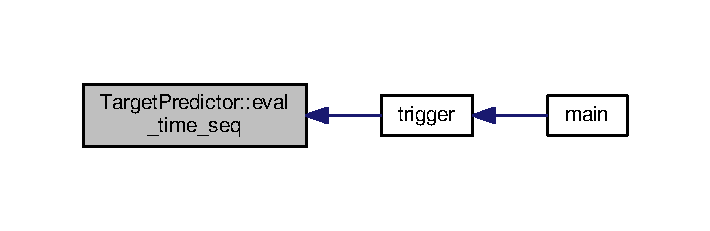
\includegraphics[width=341pt]{class_target_predictor_ac136ae7ec5c7745065f0f5662a909beb_icgraph}
\end{center}
\end{figure}


\index{Target\+Predictor@{Target\+Predictor}!get\+\_\+forecaster\+\_\+ptr@{get\+\_\+forecaster\+\_\+ptr}}
\index{get\+\_\+forecaster\+\_\+ptr@{get\+\_\+forecaster\+\_\+ptr}!Target\+Predictor@{Target\+Predictor}}
\subsubsection[{\texorpdfstring{get\+\_\+forecaster\+\_\+ptr()}{get_forecaster_ptr()}}]{\setlength{\rightskip}{0pt plus 5cm}C\+H\+O\+M\+P\+::\+Chomp\+Forecaster $\ast$ Target\+Predictor\+::get\+\_\+forecaster\+\_\+ptr (
\begin{DoxyParamCaption}
{}
\end{DoxyParamCaption}
)}\hypertarget{class_target_predictor_a56fbf63019d226246a84700c7b5f5b38}{}\label{class_target_predictor_a56fbf63019d226246a84700c7b5f5b38}


Definition at line 231 of file Target\+Manager.\+cpp.

\index{Target\+Predictor@{Target\+Predictor}!init@{init}}
\index{init@{init}!Target\+Predictor@{Target\+Predictor}}
\subsubsection[{\texorpdfstring{init()}{init()}}]{\setlength{\rightskip}{0pt plus 5cm}void Target\+Predictor\+::init (
\begin{DoxyParamCaption}
{}
\end{DoxyParamCaption}
)}\hypertarget{class_target_predictor_a3db2b852f165a35a2e709d7e2f486dde}{}\label{class_target_predictor_a3db2b852f165a35a2e709d7e2f486dde}


Definition at line 183 of file Target\+Manager.\+cpp.

\index{Target\+Predictor@{Target\+Predictor}!session@{session}}
\index{session@{session}!Target\+Predictor@{Target\+Predictor}}
\subsubsection[{\texorpdfstring{session()}{session()}}]{\setlength{\rightskip}{0pt plus 5cm}bool Target\+Predictor\+::session (
\begin{DoxyParamCaption}
{}
\end{DoxyParamCaption}
)}\hypertarget{class_target_predictor_a4468a320a84ad7abb6ed9a6e388acf1f}{}\label{class_target_predictor_a4468a320a84ad7abb6ed9a6e388acf1f}


Definition at line 255 of file Target\+Manager.\+cpp.



The documentation for this class was generated from the following files\+:\begin{DoxyCompactItemize}
\item 
include/target\+\_\+manager/\hyperlink{_target_manager_8h}{Target\+Manager.\+h}\item 
src/target\+\_\+manager/\hyperlink{_target_manager_8cpp}{Target\+Manager.\+cpp}\end{DoxyCompactItemize}

\hypertarget{class_ui___main_window}{}\section{Ui\+\_\+\+Main\+Window Class Reference}
\label{class_ui___main_window}\index{Ui\+\_\+\+Main\+Window@{Ui\+\_\+\+Main\+Window}}


Inheritance diagram for Ui\+\_\+\+Main\+Window\+:\nopagebreak
\begin{figure}[H]
\begin{center}
\leavevmode
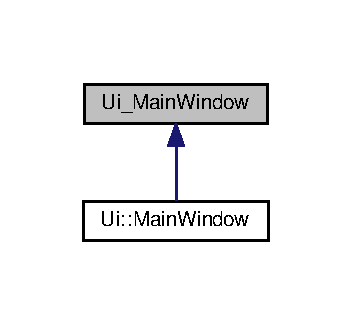
\includegraphics[width=169pt]{class_ui___main_window__inherit__graph}
\end{center}
\end{figure}
\subsection*{Public Member Functions}
\begin{DoxyCompactItemize}
\item 
void {\bfseries setup\+Ui} (Q\+Main\+Window $\ast$\hyperlink{class_main_window}{Main\+Window})\hypertarget{class_ui___main_window_acf4a0872c4c77d8f43a2ec66ed849b58}{}\label{class_ui___main_window_acf4a0872c4c77d8f43a2ec66ed849b58}

\item 
void {\bfseries retranslate\+Ui} (Q\+Main\+Window $\ast$\hyperlink{class_main_window}{Main\+Window})\hypertarget{class_ui___main_window_a097dd160c3534a204904cb374412c618}{}\label{class_ui___main_window_a097dd160c3534a204904cb374412c618}

\end{DoxyCompactItemize}
\subsection*{Public Attributes}
\begin{DoxyCompactItemize}
\item 
Q\+Widget $\ast$ {\bfseries central\+Widget}\hypertarget{class_ui___main_window_a30075506c2116c3ed4ff25e07ae75f81}{}\label{class_ui___main_window_a30075506c2116c3ed4ff25e07ae75f81}

\item 
Q\+Label $\ast$ {\bfseries label\+\_\+larr}\hypertarget{class_ui___main_window_a32587f1e879f5b685d375d2daa20f7a6}{}\label{class_ui___main_window_a32587f1e879f5b685d375d2daa20f7a6}

\item 
Q\+Label $\ast$ {\bfseries label\+\_\+larr2}\hypertarget{class_ui___main_window_a06fc1a01ac3ba3d4d1f75a0e8ab06684}{}\label{class_ui___main_window_a06fc1a01ac3ba3d4d1f75a0e8ab06684}

\item 
Q\+Label $\ast$ {\bfseries label}\hypertarget{class_ui___main_window_ad9c89133780f28e6efa2ec17ceb9cff5}{}\label{class_ui___main_window_ad9c89133780f28e6efa2ec17ceb9cff5}

\item 
Q\+Push\+Button $\ast$ {\bfseries push\+Button\+\_\+ros}\hypertarget{class_ui___main_window_a2667c2b4f9c61bf9895b73d07d4b5172}{}\label{class_ui___main_window_a2667c2b4f9c61bf9895b73d07d4b5172}

\item 
Q\+Push\+Button $\ast$ {\bfseries push\+Button\+\_\+waypoint}\hypertarget{class_ui___main_window_a6b5d7c0f96cdb3276a33746fbcd7e8c7}{}\label{class_ui___main_window_a6b5d7c0f96cdb3276a33746fbcd7e8c7}

\item 
Q\+Push\+Button $\ast$ {\bfseries push\+Button\+\_\+trajectory}\hypertarget{class_ui___main_window_a9d644554288462450d209192c1998095}{}\label{class_ui___main_window_a9d644554288462450d209192c1998095}

\item 
Q\+Push\+Button $\ast$ {\bfseries push\+Button\+\_\+simulation}\hypertarget{class_ui___main_window_afd109ead0ad1ae7ae67ad1df803c9c38}{}\label{class_ui___main_window_afd109ead0ad1ae7ae67ad1df803c9c38}

\item 
Q\+Text\+Edit $\ast$ {\bfseries text\+Edit\+\_\+board}\hypertarget{class_ui___main_window_af13441b9fd874f1aeb2ec5cefaeb0bce}{}\label{class_ui___main_window_af13441b9fd874f1aeb2ec5cefaeb0bce}

\item 
Q\+Push\+Button $\ast$ {\bfseries push\+Button\+\_\+save}\hypertarget{class_ui___main_window_a257d4df0fe652a526e4fddba93c7a7d8}{}\label{class_ui___main_window_a257d4df0fe652a526e4fddba93c7a7d8}

\item 
Q\+Line\+Edit $\ast$ {\bfseries line\+Edit\+\_\+logging\+\_\+dir}\hypertarget{class_ui___main_window_a7ab71242b81ef9d13f83c16f6328f35d}{}\label{class_ui___main_window_a7ab71242b81ef9d13f83c16f6328f35d}

\item 
Q\+Label $\ast$ {\bfseries label\+\_\+2}\hypertarget{class_ui___main_window_a2e2516d755e4dd53fc905dabddf2738a}{}\label{class_ui___main_window_a2e2516d755e4dd53fc905dabddf2738a}

\item 
Q\+Label $\ast$ {\bfseries label\+\_\+3}\hypertarget{class_ui___main_window_a0376fd90247280e7c7957cc70628708c}{}\label{class_ui___main_window_a0376fd90247280e7c7957cc70628708c}

\item 
Q\+Line\+Edit $\ast$ {\bfseries line\+Edit\+\_\+target\+\_\+trajectory}\hypertarget{class_ui___main_window_a4a75bfb754049f89fccef822cad712d6}{}\label{class_ui___main_window_a4a75bfb754049f89fccef822cad712d6}

\item 
Q\+Push\+Button $\ast$ {\bfseries push\+Button\+\_\+load}\hypertarget{class_ui___main_window_a67832089879377ce16b3f26fbb2cc3f2}{}\label{class_ui___main_window_a67832089879377ce16b3f26fbb2cc3f2}

\item 
Q\+Push\+Button $\ast$ {\bfseries push\+Button\+\_\+clear}\hypertarget{class_ui___main_window_a5d7af3b0fdbc605e3fd8ae6ceffa0d29}{}\label{class_ui___main_window_a5d7af3b0fdbc605e3fd8ae6ceffa0d29}

\item 
Q\+Push\+Button $\ast$ {\bfseries push\+Button\+\_\+undo}\hypertarget{class_ui___main_window_ab3fd048b1a1dee328d8e1b433955bf29}{}\label{class_ui___main_window_ab3fd048b1a1dee328d8e1b433955bf29}

\item 
Q\+Label $\ast$ {\bfseries label\+\_\+4}\hypertarget{class_ui___main_window_a78c7e10730b43c6700cd7216911ed76a}{}\label{class_ui___main_window_a78c7e10730b43c6700cd7216911ed76a}

\item 
Q\+Line\+Edit $\ast$ {\bfseries line\+Edit\+\_\+tf}\hypertarget{class_ui___main_window_afc0d94ce5096c619c413cfae9b62014c}{}\label{class_ui___main_window_afc0d94ce5096c619c413cfae9b62014c}

\item 
Q\+Push\+Button $\ast$ {\bfseries push\+Button\+\_\+chaser}\hypertarget{class_ui___main_window_a9e8499b7c9a9717499abde993da72ed5}{}\label{class_ui___main_window_a9e8499b7c9a9717499abde993da72ed5}

\item 
Q\+Menu\+Bar $\ast$ {\bfseries menu\+Bar}\hypertarget{class_ui___main_window_a2be1c24ec9adfca18e1dcc951931457f}{}\label{class_ui___main_window_a2be1c24ec9adfca18e1dcc951931457f}

\item 
Q\+Menu $\ast$ {\bfseries menu\+Auto\+\_\+chaser}\hypertarget{class_ui___main_window_a8946bc17fa5b33e1c89ef82fdacab1d8}{}\label{class_ui___main_window_a8946bc17fa5b33e1c89ef82fdacab1d8}

\item 
Q\+Tool\+Bar $\ast$ {\bfseries main\+Tool\+Bar}\hypertarget{class_ui___main_window_a5172877001c8c7b4e0f6de50421867d1}{}\label{class_ui___main_window_a5172877001c8c7b4e0f6de50421867d1}

\item 
Q\+Status\+Bar $\ast$ {\bfseries status\+Bar}\hypertarget{class_ui___main_window_a50fa481337604bcc8bf68de18ab16ecd}{}\label{class_ui___main_window_a50fa481337604bcc8bf68de18ab16ecd}

\end{DoxyCompactItemize}


The documentation for this class was generated from the following file\+:\begin{DoxyCompactItemize}
\item 
src/build-\/qt\+\_\+ui-\/\+Desktop-\/\+Debug/ui\+\_\+mainwindow.\+h\end{DoxyCompactItemize}

\hypertarget{class_wrapper}{}\section{Wrapper Class Reference}
\label{class_wrapper}\index{Wrapper@{Wrapper}}


{\ttfamily \#include $<$Wrapper.\+h$>$}



Collaboration diagram for Wrapper\+:
\nopagebreak
\begin{figure}[H]
\begin{center}
\leavevmode
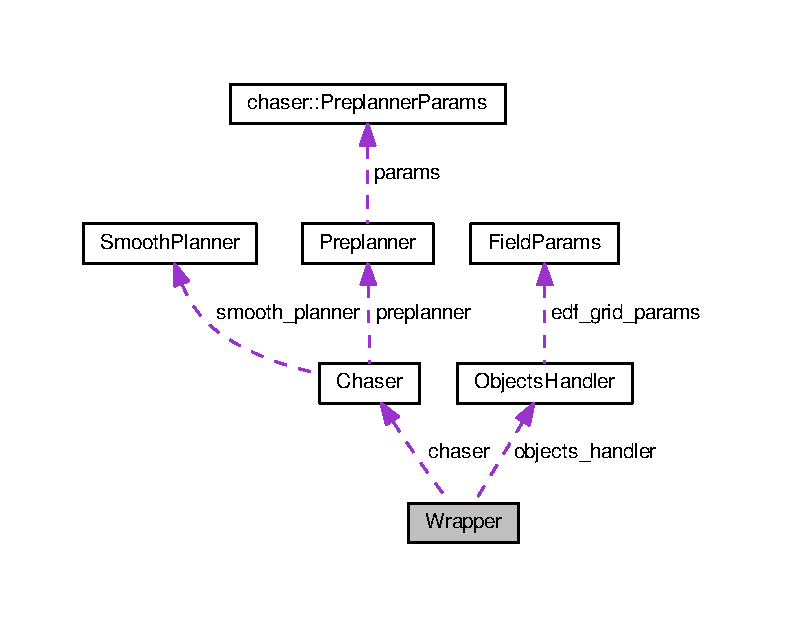
\includegraphics[width=243pt]{class_wrapper__coll__graph}
\end{center}
\end{figure}
\subsection*{Public Member Functions}
\begin{DoxyCompactItemize}
\item 
\hyperlink{class_wrapper_aa40ce9fcba8ab60bf01bcb0913144b4a}{Wrapper} ()
\item 
void \hyperlink{class_wrapper_af336781e7d75d525e7b152366a0e0d93}{init} (ros\+::\+Node\+Handle nh)
\item 
void \hyperlink{class_wrapper_a009ee5c325926f92df42319d5469a376}{session} (double t)
\item 
bool \hyperlink{class_wrapper_a21a0e115ea80e053e4f2defd1362b92f}{trigger\+\_\+chasing} (Time\+Series chasing\+\_\+knots)
\item 
bool \hyperlink{class_wrapper_a2da6448c77dd4edb054de4130b1fc883}{trigger\+\_\+chasing} (vector$<$ Point $>$ target\+\_\+seq, Time\+Series chasing\+\_\+knots)
\item 
geometry\+\_\+msgs\+::\+Pose\+Stamped \hyperlink{class_wrapper_ac2338df9e7b31f3291ed1cbd137a6f14}{get\+\_\+control\+\_\+pose} (double t\+\_\+eval)
\begin{DoxyCompactList}\small\item\em evalate the latest control pose from chaser \end{DoxyCompactList}\item 
void \hyperlink{class_wrapper_a94a786272ea8120469cb476d021c5b76}{pub\+\_\+control\+\_\+pose} (double t\+\_\+eval)
\begin{DoxyCompactList}\small\item\em publish the control visualization (geometry\+\_\+msgs) \end{DoxyCompactList}\item 
void \hyperlink{class_wrapper_a7f0e09c8a675991a3c987e41c6b9ff9d}{pub\+\_\+control\+\_\+traj} (double t\+\_\+eval)
\begin{DoxyCompactList}\small\item\em publish the control visualization (trajectory\+\_\+msgs) \end{DoxyCompactList}\item 
void \hyperlink{class_wrapper_a3fcc1a8192f2e72f501f2e9912a0ef41}{pub\+\_\+control\+\_\+pose} (Pose\+Stamped control\+\_\+pose)
\item 
void \hyperlink{class_wrapper_a754999f67924fbda6dc3b3e38377af79}{pub\+\_\+control\+\_\+traj} (Pose\+Stamped control\+\_\+pose)
\end{DoxyCompactItemize}
\subsection*{Public Attributes}
\begin{DoxyCompactItemize}
\item 
int \hyperlink{class_wrapper_a4b4e8407edf38f99eb9d5a0cd4a0116b}{run\+\_\+mode}
\item 
\hyperlink{class_objects_handler}{Objects\+Handler} \hyperlink{class_wrapper_a8cddd5ffbaeb5ab0b5d8d8d0c74f810f}{objects\+\_\+handler}
\item 
\hyperlink{class_chaser}{Chaser} \hyperlink{class_wrapper_a750309ad3470e20a80e9d72b0d7e34cb}{chaser}
\end{DoxyCompactItemize}


\subsection{Detailed Description}


Definition at line 6 of file Wrapper.\+h.



\subsection{Constructor \& Destructor Documentation}
\index{Wrapper@{Wrapper}!Wrapper@{Wrapper}}
\index{Wrapper@{Wrapper}!Wrapper@{Wrapper}}
\subsubsection[{\texorpdfstring{Wrapper()}{Wrapper()}}]{\setlength{\rightskip}{0pt plus 5cm}Wrapper\+::\+Wrapper (
\begin{DoxyParamCaption}
{}
\end{DoxyParamCaption}
)}\hypertarget{class_wrapper_aa40ce9fcba8ab60bf01bcb0913144b4a}{}\label{class_wrapper_aa40ce9fcba8ab60bf01bcb0913144b4a}


Definition at line 3 of file Wrapper.\+cpp.



\subsection{Member Function Documentation}
\index{Wrapper@{Wrapper}!get\+\_\+control\+\_\+pose@{get\+\_\+control\+\_\+pose}}
\index{get\+\_\+control\+\_\+pose@{get\+\_\+control\+\_\+pose}!Wrapper@{Wrapper}}
\subsubsection[{\texorpdfstring{get\+\_\+control\+\_\+pose(double t\+\_\+eval)}{get_control_pose(double t_eval)}}]{\setlength{\rightskip}{0pt plus 5cm}geometry\+\_\+msgs\+::\+Pose\+Stamped Wrapper\+::get\+\_\+control\+\_\+pose (
\begin{DoxyParamCaption}
\item[{double}]{t\+\_\+eval}
\end{DoxyParamCaption}
)}\hypertarget{class_wrapper_ac2338df9e7b31f3291ed1cbd137a6f14}{}\label{class_wrapper_ac2338df9e7b31f3291ed1cbd137a6f14}


evalate the latest control pose from chaser 


\begin{DoxyParams}{Parameters}
{\em t\+\_\+eval} & the evaluation time \\
\hline
\end{DoxyParams}
\begin{DoxyReturn}{Returns}
geometry\+\_\+msgs\+::\+Pose\+Stamped the control pose for M\+AV 
\end{DoxyReturn}


Definition at line 131 of file Wrapper.\+cpp.



Here is the call graph for this function\+:
\nopagebreak
\begin{figure}[H]
\begin{center}
\leavevmode
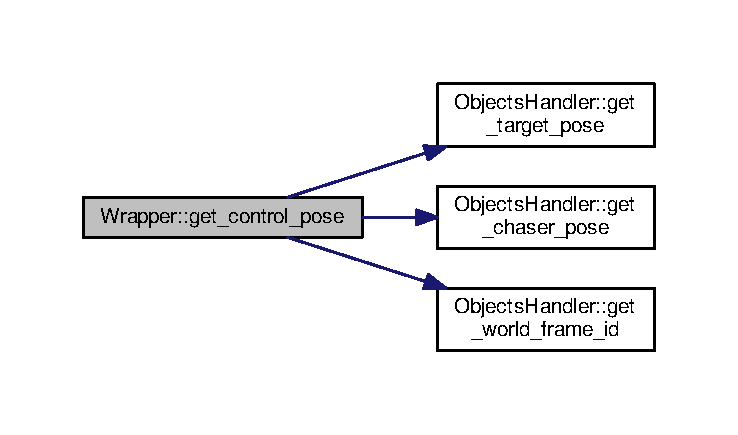
\includegraphics[width=350pt]{class_wrapper_ac2338df9e7b31f3291ed1cbd137a6f14_cgraph}
\end{center}
\end{figure}




Here is the caller graph for this function\+:
\nopagebreak
\begin{figure}[H]
\begin{center}
\leavevmode
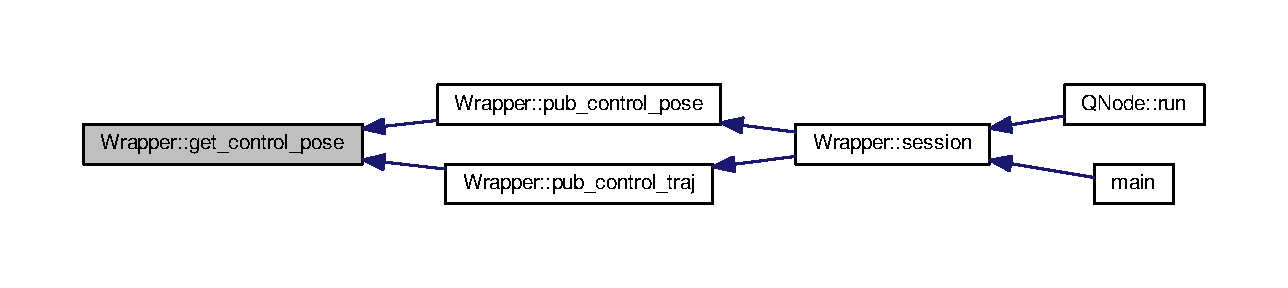
\includegraphics[width=350pt]{class_wrapper_ac2338df9e7b31f3291ed1cbd137a6f14_icgraph}
\end{center}
\end{figure}


\index{Wrapper@{Wrapper}!init@{init}}
\index{init@{init}!Wrapper@{Wrapper}}
\subsubsection[{\texorpdfstring{init(ros\+::\+Node\+Handle nh)}{init(ros::NodeHandle nh)}}]{\setlength{\rightskip}{0pt plus 5cm}void Wrapper\+::init (
\begin{DoxyParamCaption}
\item[{ros\+::\+Node\+Handle}]{nh}
\end{DoxyParamCaption}
)}\hypertarget{class_wrapper_af336781e7d75d525e7b152366a0e0d93}{}\label{class_wrapper_af336781e7d75d525e7b152366a0e0d93}


Definition at line 5 of file Wrapper.\+cpp.



Here is the call graph for this function\+:
\nopagebreak
\begin{figure}[H]
\begin{center}
\leavevmode
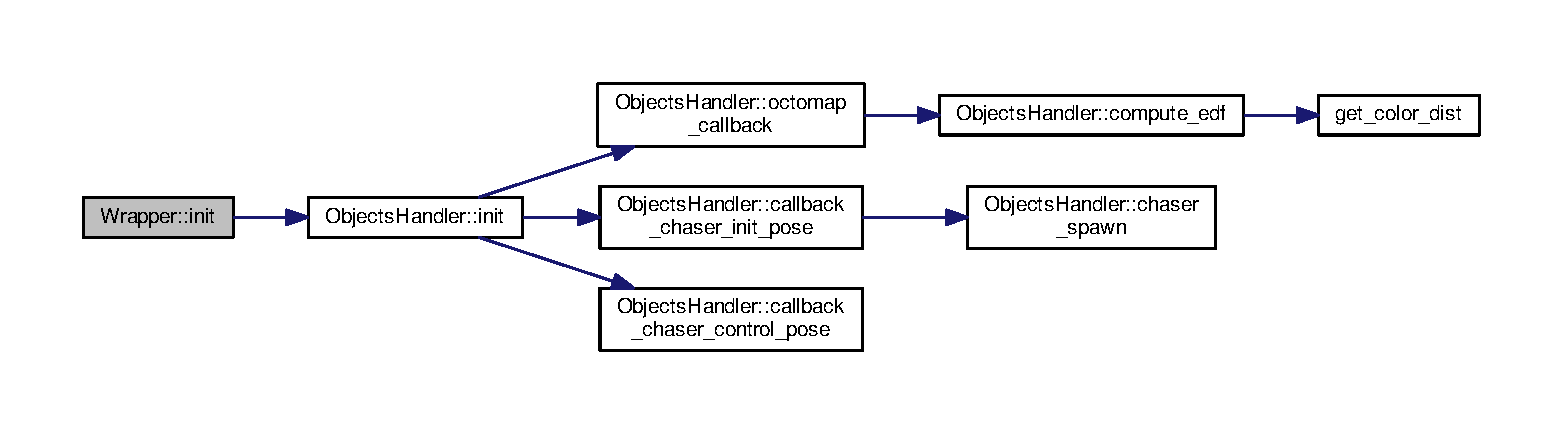
\includegraphics[width=350pt]{class_wrapper_af336781e7d75d525e7b152366a0e0d93_cgraph}
\end{center}
\end{figure}




Here is the caller graph for this function\+:
\nopagebreak
\begin{figure}[H]
\begin{center}
\leavevmode
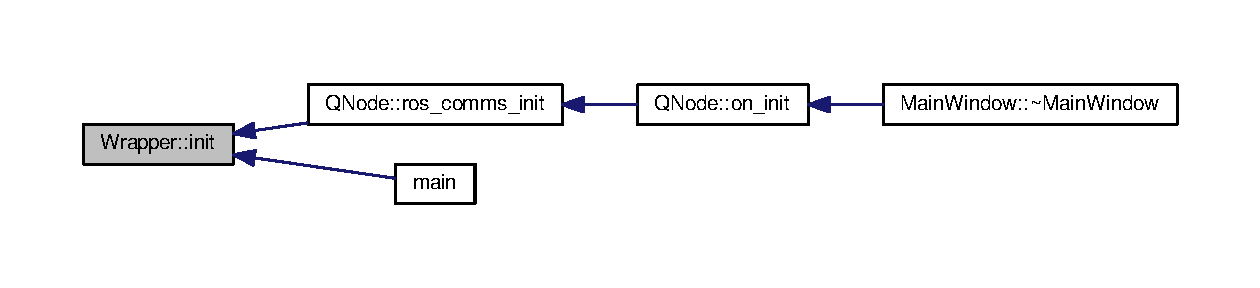
\includegraphics[width=350pt]{class_wrapper_af336781e7d75d525e7b152366a0e0d93_icgraph}
\end{center}
\end{figure}


\index{Wrapper@{Wrapper}!pub\+\_\+control\+\_\+pose@{pub\+\_\+control\+\_\+pose}}
\index{pub\+\_\+control\+\_\+pose@{pub\+\_\+control\+\_\+pose}!Wrapper@{Wrapper}}
\subsubsection[{\texorpdfstring{pub\+\_\+control\+\_\+pose(double t\+\_\+eval)}{pub_control_pose(double t_eval)}}]{\setlength{\rightskip}{0pt plus 5cm}void Wrapper\+::pub\+\_\+control\+\_\+pose (
\begin{DoxyParamCaption}
\item[{double}]{t\+\_\+eval}
\end{DoxyParamCaption}
)}\hypertarget{class_wrapper_a94a786272ea8120469cb476d021c5b76}{}\label{class_wrapper_a94a786272ea8120469cb476d021c5b76}


publish the control visualization (geometry\+\_\+msgs) 


\begin{DoxyParams}{Parameters}
{\em t\+\_\+eval} & evaluation time \\
\hline
\end{DoxyParams}


Definition at line 222 of file Wrapper.\+cpp.



Here is the call graph for this function\+:
\nopagebreak
\begin{figure}[H]
\begin{center}
\leavevmode
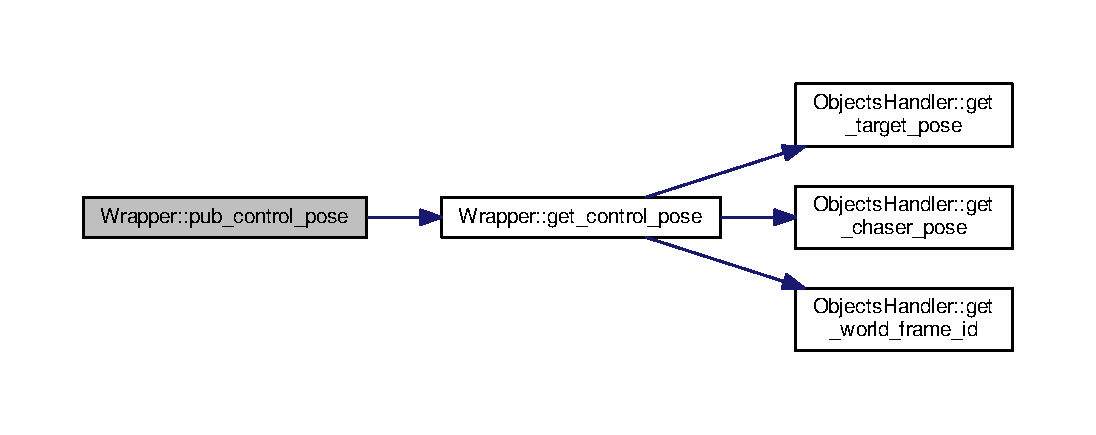
\includegraphics[width=350pt]{class_wrapper_a94a786272ea8120469cb476d021c5b76_cgraph}
\end{center}
\end{figure}




Here is the caller graph for this function\+:
\nopagebreak
\begin{figure}[H]
\begin{center}
\leavevmode
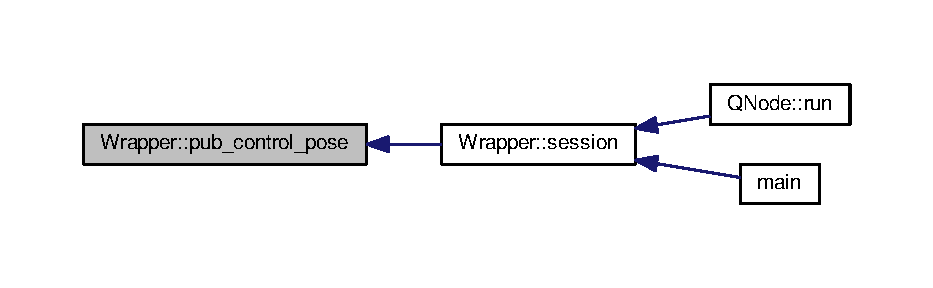
\includegraphics[width=350pt]{class_wrapper_a94a786272ea8120469cb476d021c5b76_icgraph}
\end{center}
\end{figure}


\index{Wrapper@{Wrapper}!pub\+\_\+control\+\_\+pose@{pub\+\_\+control\+\_\+pose}}
\index{pub\+\_\+control\+\_\+pose@{pub\+\_\+control\+\_\+pose}!Wrapper@{Wrapper}}
\subsubsection[{\texorpdfstring{pub\+\_\+control\+\_\+pose(\+Pose\+Stamped control\+\_\+pose)}{pub_control_pose(PoseStamped control_pose)}}]{\setlength{\rightskip}{0pt plus 5cm}void Wrapper\+::pub\+\_\+control\+\_\+pose (
\begin{DoxyParamCaption}
\item[{Pose\+Stamped}]{control\+\_\+pose}
\end{DoxyParamCaption}
)}\hypertarget{class_wrapper_a3fcc1a8192f2e72f501f2e9912a0ef41}{}\label{class_wrapper_a3fcc1a8192f2e72f501f2e9912a0ef41}
\index{Wrapper@{Wrapper}!pub\+\_\+control\+\_\+traj@{pub\+\_\+control\+\_\+traj}}
\index{pub\+\_\+control\+\_\+traj@{pub\+\_\+control\+\_\+traj}!Wrapper@{Wrapper}}
\subsubsection[{\texorpdfstring{pub\+\_\+control\+\_\+traj(double t\+\_\+eval)}{pub_control_traj(double t_eval)}}]{\setlength{\rightskip}{0pt plus 5cm}void Wrapper\+::pub\+\_\+control\+\_\+traj (
\begin{DoxyParamCaption}
\item[{double}]{t\+\_\+eval}
\end{DoxyParamCaption}
)}\hypertarget{class_wrapper_a7f0e09c8a675991a3c987e41c6b9ff9d}{}\label{class_wrapper_a7f0e09c8a675991a3c987e41c6b9ff9d}


publish the control visualization (trajectory\+\_\+msgs) 


\begin{DoxyParams}{Parameters}
{\em t\+\_\+eval} & \\
\hline
\end{DoxyParams}


Definition at line 235 of file Wrapper.\+cpp.



Here is the call graph for this function\+:
\nopagebreak
\begin{figure}[H]
\begin{center}
\leavevmode
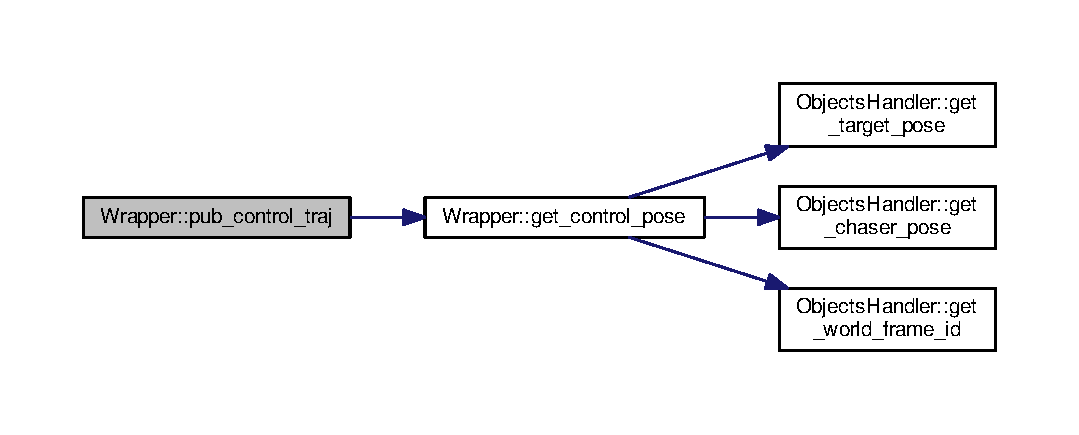
\includegraphics[width=350pt]{class_wrapper_a7f0e09c8a675991a3c987e41c6b9ff9d_cgraph}
\end{center}
\end{figure}




Here is the caller graph for this function\+:
\nopagebreak
\begin{figure}[H]
\begin{center}
\leavevmode
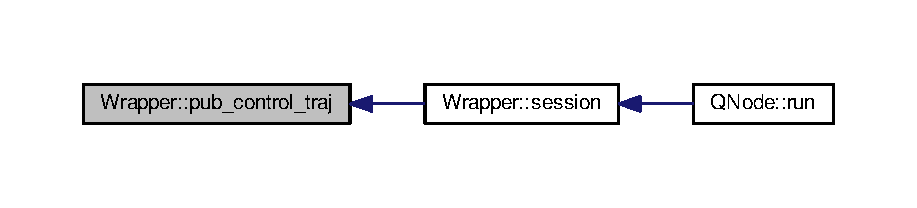
\includegraphics[width=350pt]{class_wrapper_a7f0e09c8a675991a3c987e41c6b9ff9d_icgraph}
\end{center}
\end{figure}


\index{Wrapper@{Wrapper}!pub\+\_\+control\+\_\+traj@{pub\+\_\+control\+\_\+traj}}
\index{pub\+\_\+control\+\_\+traj@{pub\+\_\+control\+\_\+traj}!Wrapper@{Wrapper}}
\subsubsection[{\texorpdfstring{pub\+\_\+control\+\_\+traj(\+Pose\+Stamped control\+\_\+pose)}{pub_control_traj(PoseStamped control_pose)}}]{\setlength{\rightskip}{0pt plus 5cm}void Wrapper\+::pub\+\_\+control\+\_\+traj (
\begin{DoxyParamCaption}
\item[{Pose\+Stamped}]{control\+\_\+pose}
\end{DoxyParamCaption}
)}\hypertarget{class_wrapper_a754999f67924fbda6dc3b3e38377af79}{}\label{class_wrapper_a754999f67924fbda6dc3b3e38377af79}
\index{Wrapper@{Wrapper}!session@{session}}
\index{session@{session}!Wrapper@{Wrapper}}
\subsubsection[{\texorpdfstring{session(double t)}{session(double t)}}]{\setlength{\rightskip}{0pt plus 5cm}void Wrapper\+::session (
\begin{DoxyParamCaption}
\item[{double}]{t}
\end{DoxyParamCaption}
)}\hypertarget{class_wrapper_a009ee5c325926f92df42319d5469a376}{}\label{class_wrapper_a009ee5c325926f92df42319d5469a376}


Definition at line 28 of file Wrapper.\+cpp.



Here is the call graph for this function\+:
\nopagebreak
\begin{figure}[H]
\begin{center}
\leavevmode
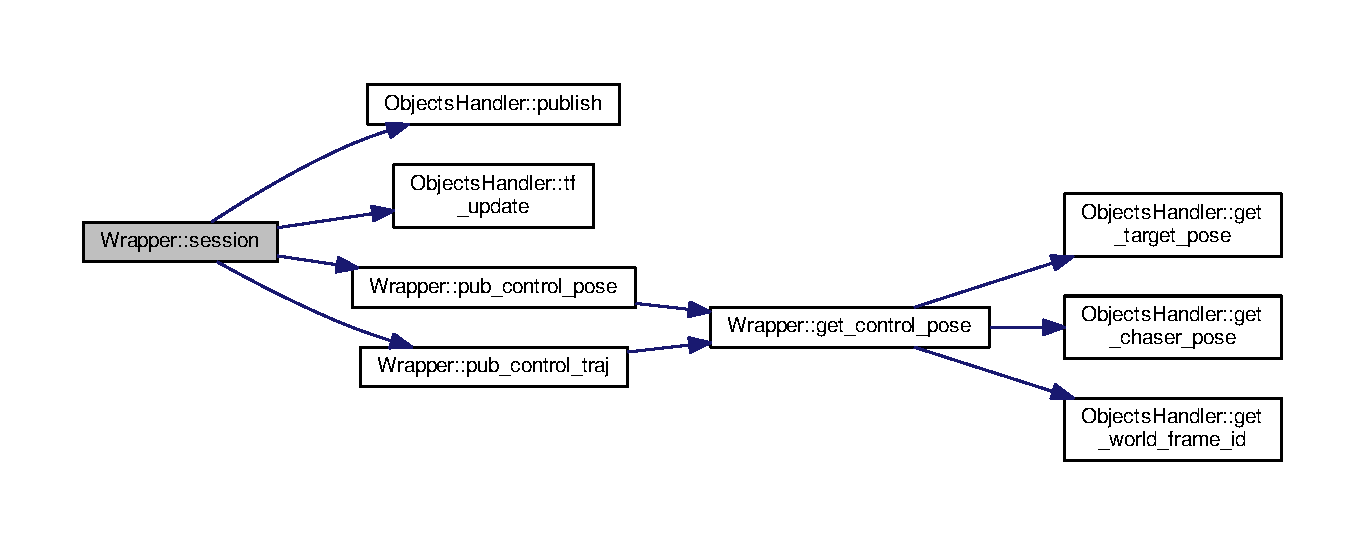
\includegraphics[width=350pt]{class_wrapper_a009ee5c325926f92df42319d5469a376_cgraph}
\end{center}
\end{figure}




Here is the caller graph for this function\+:
\nopagebreak
\begin{figure}[H]
\begin{center}
\leavevmode
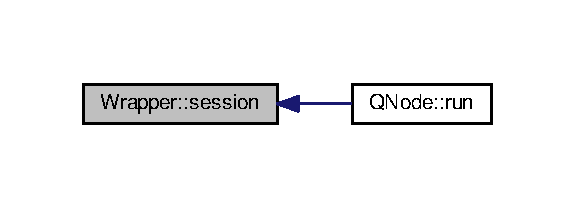
\includegraphics[width=276pt]{class_wrapper_a009ee5c325926f92df42319d5469a376_icgraph}
\end{center}
\end{figure}


\index{Wrapper@{Wrapper}!trigger\+\_\+chasing@{trigger\+\_\+chasing}}
\index{trigger\+\_\+chasing@{trigger\+\_\+chasing}!Wrapper@{Wrapper}}
\subsubsection[{\texorpdfstring{trigger\+\_\+chasing(\+Time\+Series chasing\+\_\+knots)}{trigger_chasing(TimeSeries chasing_knots)}}]{\setlength{\rightskip}{0pt plus 5cm}bool Wrapper\+::trigger\+\_\+chasing (
\begin{DoxyParamCaption}
\item[{Time\+Series}]{chasing\+\_\+knots}
\end{DoxyParamCaption}
)}\hypertarget{class_wrapper_a21a0e115ea80e053e4f2defd1362b92f}{}\label{class_wrapper_a21a0e115ea80e053e4f2defd1362b92f}


Definition at line 59 of file Wrapper.\+cpp.



Here is the call graph for this function\+:
\nopagebreak
\begin{figure}[H]
\begin{center}
\leavevmode
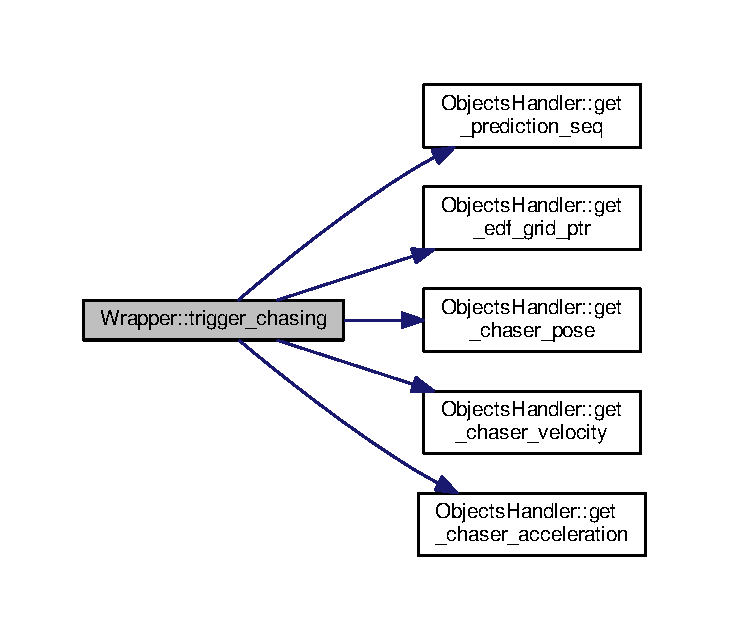
\includegraphics[width=350pt]{class_wrapper_a21a0e115ea80e053e4f2defd1362b92f_cgraph}
\end{center}
\end{figure}




Here is the caller graph for this function\+:
\nopagebreak
\begin{figure}[H]
\begin{center}
\leavevmode
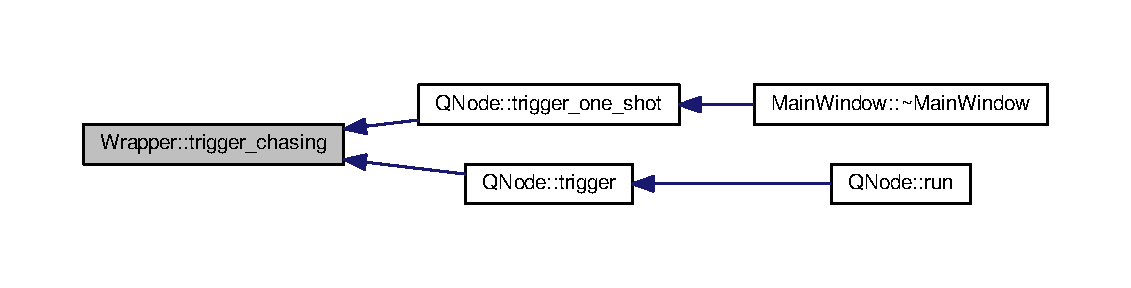
\includegraphics[width=350pt]{class_wrapper_a21a0e115ea80e053e4f2defd1362b92f_icgraph}
\end{center}
\end{figure}


\index{Wrapper@{Wrapper}!trigger\+\_\+chasing@{trigger\+\_\+chasing}}
\index{trigger\+\_\+chasing@{trigger\+\_\+chasing}!Wrapper@{Wrapper}}
\subsubsection[{\texorpdfstring{trigger\+\_\+chasing(vector$<$ Point $>$ target\+\_\+seq, Time\+Series chasing\+\_\+knots)}{trigger_chasing(vector< Point > target_seq, TimeSeries chasing_knots)}}]{\setlength{\rightskip}{0pt plus 5cm}bool Wrapper\+::trigger\+\_\+chasing (
\begin{DoxyParamCaption}
\item[{vector$<$ Point $>$}]{target\+\_\+seq, }
\item[{Time\+Series}]{chasing\+\_\+knots}
\end{DoxyParamCaption}
)}\hypertarget{class_wrapper_a2da6448c77dd4edb054de4130b1fc883}{}\label{class_wrapper_a2da6448c77dd4edb054de4130b1fc883}


Definition at line 92 of file Wrapper.\+cpp.



Here is the call graph for this function\+:
\nopagebreak
\begin{figure}[H]
\begin{center}
\leavevmode
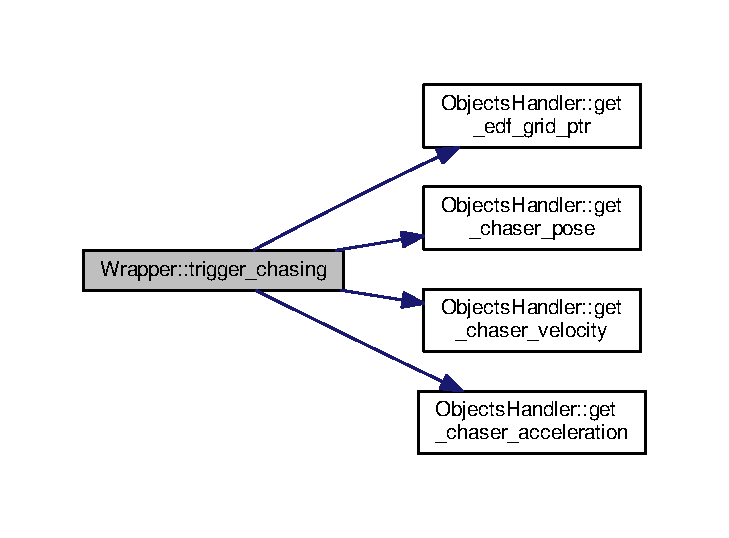
\includegraphics[width=350pt]{class_wrapper_a2da6448c77dd4edb054de4130b1fc883_cgraph}
\end{center}
\end{figure}




\subsection{Member Data Documentation}
\index{Wrapper@{Wrapper}!chaser@{chaser}}
\index{chaser@{chaser}!Wrapper@{Wrapper}}
\subsubsection[{\texorpdfstring{chaser}{chaser}}]{\setlength{\rightskip}{0pt plus 5cm}{\bf Chaser} Wrapper\+::chaser}\hypertarget{class_wrapper_a750309ad3470e20a80e9d72b0d7e34cb}{}\label{class_wrapper_a750309ad3470e20a80e9d72b0d7e34cb}


Definition at line 31 of file Wrapper.\+h.

\index{Wrapper@{Wrapper}!objects\+\_\+handler@{objects\+\_\+handler}}
\index{objects\+\_\+handler@{objects\+\_\+handler}!Wrapper@{Wrapper}}
\subsubsection[{\texorpdfstring{objects\+\_\+handler}{objects_handler}}]{\setlength{\rightskip}{0pt plus 5cm}{\bf Objects\+Handler} Wrapper\+::objects\+\_\+handler}\hypertarget{class_wrapper_a8cddd5ffbaeb5ab0b5d8d8d0c74f810f}{}\label{class_wrapper_a8cddd5ffbaeb5ab0b5d8d8d0c74f810f}


Definition at line 30 of file Wrapper.\+h.

\index{Wrapper@{Wrapper}!run\+\_\+mode@{run\+\_\+mode}}
\index{run\+\_\+mode@{run\+\_\+mode}!Wrapper@{Wrapper}}
\subsubsection[{\texorpdfstring{run\+\_\+mode}{run_mode}}]{\setlength{\rightskip}{0pt plus 5cm}int Wrapper\+::run\+\_\+mode}\hypertarget{class_wrapper_a4b4e8407edf38f99eb9d5a0cd4a0116b}{}\label{class_wrapper_a4b4e8407edf38f99eb9d5a0cd4a0116b}


Definition at line 29 of file Wrapper.\+h.



The documentation for this class was generated from the following files\+:\begin{DoxyCompactItemize}
\item 
include/auto\+\_\+chaser/\hyperlink{_wrapper_8h}{Wrapper.\+h}\item 
src/auto\+\_\+chaser/\hyperlink{_wrapper_8cpp}{Wrapper.\+cpp}\end{DoxyCompactItemize}

\chapter{File Documentation}
\hypertarget{generate__cached__setup_8py}{}\section{build/catkin\+\_\+generated/generate\+\_\+cached\+\_\+setup.py File Reference}
\label{generate__cached__setup_8py}\index{build/catkin\+\_\+generated/generate\+\_\+cached\+\_\+setup.\+py@{build/catkin\+\_\+generated/generate\+\_\+cached\+\_\+setup.\+py}}
\subsection*{Namespaces}
\begin{DoxyCompactItemize}
\item 
 \hyperlink{namespacegenerate__cached__setup}{generate\+\_\+cached\+\_\+setup}
\end{DoxyCompactItemize}
\subsection*{Variables}
\begin{DoxyCompactItemize}
\item 
\hyperlink{namespacegenerate__cached__setup_a72579fd01529a79bab20d99291889d3f}{generate\+\_\+cached\+\_\+setup.\+python\+\_\+path} = os.\+path.\+join(workspace, \textquotesingle{}lib/python2.\+7/dist-\/packages\textquotesingle{})
\item 
\hyperlink{namespacegenerate__cached__setup_a52601295006f2366a311c4453d8f2f2e}{generate\+\_\+cached\+\_\+setup.\+code} = generate\+\_\+environment\+\_\+script(\textquotesingle{}/home/jbs/catkin\+\_\+ws/src/auto\+\_\+chaser/build/devel/env.\+sh\textquotesingle{})
\item 
string \hyperlink{namespacegenerate__cached__setup_a0265aee5075ee1eb701ff69c98ad6793}{generate\+\_\+cached\+\_\+setup.\+output\+\_\+filename} = \textquotesingle{}/home/jbs/catkin\+\_\+ws/src/auto\+\_\+chaser/build/catkin\+\_\+generated/setup\+\_\+cached.\+sh\textquotesingle{}
\item 
\hyperlink{namespacegenerate__cached__setup_a10081e5abedae9bd46dd91202096e789}{generate\+\_\+cached\+\_\+setup.\+mode} = os.\+stat(output\+\_\+filename).st\+\_\+mode
\end{DoxyCompactItemize}

\hypertarget{catkin__generated_2installspace_2__setup__util_8py}{}\section{build/catkin\+\_\+generated/installspace/\+\_\+setup\+\_\+util.py File Reference}
\label{catkin__generated_2installspace_2__setup__util_8py}\index{build/catkin\+\_\+generated/installspace/\+\_\+setup\+\_\+util.\+py@{build/catkin\+\_\+generated/installspace/\+\_\+setup\+\_\+util.\+py}}
\subsection*{Namespaces}
\begin{DoxyCompactItemize}
\item 
 \hyperlink{namespace__setup__util}{\+\_\+setup\+\_\+util}
\end{DoxyCompactItemize}
\subsection*{Functions}
\begin{DoxyCompactItemize}
\item 
def \hyperlink{namespace__setup__util_af3030db6102b5aa35cd354a2fb6cca03}{\+\_\+setup\+\_\+util.\+rollback\+\_\+env\+\_\+variables} (environ, env\+\_\+var\+\_\+subfolders)
\item 
def \hyperlink{namespace__setup__util_af05661e87b3270e8bfd0fbc18a5eeec4}{\+\_\+setup\+\_\+util.\+\_\+rollback\+\_\+env\+\_\+variable} (environ, name, subfolders)
\item 
def \hyperlink{namespace__setup__util_ab2be07aa31918f1e1e34d6b7c4d66fcb}{\+\_\+setup\+\_\+util.\+\_\+get\+\_\+workspaces} (environ, include\+\_\+fuerte=False, include\+\_\+non\+\_\+existing=False)
\item 
def \hyperlink{namespace__setup__util_a832417d18b85bd1d276a87547e86f860}{\+\_\+setup\+\_\+util.\+prepend\+\_\+env\+\_\+variables} (environ, env\+\_\+var\+\_\+subfolders, workspaces)
\item 
def \hyperlink{namespace__setup__util_a74a1f8575ed82282d03f7795c9ba6e45}{\+\_\+setup\+\_\+util.\+\_\+prefix\+\_\+env\+\_\+variable} (environ, name, paths, subfolders)
\item 
def \hyperlink{namespace__setup__util_ad56c24837fa4eddc63c03fbc7035628f}{\+\_\+setup\+\_\+util.\+assignment} (key, value)
\item 
def \hyperlink{namespace__setup__util_abe8c95c4cfe8b1374dacd5f91d984353}{\+\_\+setup\+\_\+util.\+comment} (msg)
\item 
def \hyperlink{namespace__setup__util_ae78d86b2c4279f5b8b1acaa146c35802}{\+\_\+setup\+\_\+util.\+prepend} (environ, key, prefix)
\item 
def \hyperlink{namespace__setup__util_a73de35ca77f260af6691470342ab49ce}{\+\_\+setup\+\_\+util.\+find\+\_\+env\+\_\+hooks} (environ, cmake\+\_\+prefix\+\_\+path)
\item 
def \hyperlink{namespace__setup__util_a57d9ecb280810c9a5409d44aeb9d0a25}{\+\_\+setup\+\_\+util.\+\_\+parse\+\_\+arguments} (args=None)
\end{DoxyCompactItemize}
\subsection*{Variables}
\begin{DoxyCompactItemize}
\item 
string \hyperlink{namespace__setup__util_a3fa0ca5a460a71a43cbc3d4954ab1f10}{\+\_\+setup\+\_\+util.\+C\+A\+T\+K\+I\+N\+\_\+\+M\+A\+R\+K\+E\+R\+\_\+\+F\+I\+LE} = \textquotesingle{}.catkin\textquotesingle{}
\item 
\hyperlink{namespace__setup__util_ae9fca6a80a6923f4580be72f68fee325}{\+\_\+setup\+\_\+util.\+system} = platform.\+system()
\item 
tuple \hyperlink{namespace__setup__util_aecbb100ce6f94bb3c7e16d58fde05f96}{\+\_\+setup\+\_\+util.\+I\+S\+\_\+\+D\+A\+R\+W\+IN} = (system == \textquotesingle{}Darwin\textquotesingle{})
\item 
tuple \hyperlink{namespace__setup__util_a6fe69c2dbd92959b6651a28cbb846e6e}{\+\_\+setup\+\_\+util.\+I\+S\+\_\+\+W\+I\+N\+D\+O\+WS} = (system == \textquotesingle{}Windows\textquotesingle{})
\item 
dictionary \hyperlink{namespace__setup__util_aa31804f1be8660156ce9394b33c68dc4}{\+\_\+setup\+\_\+util.\+E\+N\+V\+\_\+\+V\+A\+R\+\_\+\+S\+U\+B\+F\+O\+L\+D\+E\+RS}
\item 
\hyperlink{namespace__setup__util_a547963d07c6371df1c51b1384a2dec28}{\+\_\+setup\+\_\+util.\+args} = \+\_\+parse\+\_\+arguments()
\item 
\hyperlink{namespace__setup__util_acdce690b925de33d6249bbbfa1109d61}{\+\_\+setup\+\_\+util.\+e}
\item 
\hyperlink{namespace__setup__util_aea63a1b32cc79bc3d872ab7cb30dd07e}{\+\_\+setup\+\_\+util.\+file}
\item 
string \hyperlink{namespace__setup__util_a57afd3d2c076955fb715f3e72ef098eb}{\+\_\+setup\+\_\+util.\+C\+M\+A\+K\+E\+\_\+\+P\+R\+E\+F\+I\+X\+\_\+\+P\+A\+TH} = \textquotesingle{}/home/jbs/catkin\+\_\+ws/devel;/opt/ros/kinetic\textquotesingle{}
\item 
\hyperlink{namespace__setup__util_a83d25140acd7788bbcb95843fe38e639}{\+\_\+setup\+\_\+util.\+base\+\_\+path} = os.\+path.\+dirname(\+\_\+\+\_\+file\+\_\+\+\_\+)
\item 
\hyperlink{namespace__setup__util_a9a935bdd9ee1aa0327161025bb18c136}{\+\_\+setup\+\_\+util.\+environ} = dict(os.\+environ)
\item 
list \hyperlink{namespace__setup__util_a8618d8be5f729d4c9696daa5e083a001}{\+\_\+setup\+\_\+util.\+lines} = \mbox{[}$\,$\mbox{]}
\end{DoxyCompactItemize}

\hypertarget{devel_2__setup__util_8py}{}\section{build/devel/\+\_\+setup\+\_\+util.py File Reference}
\label{devel_2__setup__util_8py}\index{build/devel/\+\_\+setup\+\_\+util.\+py@{build/devel/\+\_\+setup\+\_\+util.\+py}}
\subsection*{Namespaces}
\begin{DoxyCompactItemize}
\item 
 \hyperlink{namespace__setup__util}{\+\_\+setup\+\_\+util}
\end{DoxyCompactItemize}
\subsection*{Functions}
\begin{DoxyCompactItemize}
\item 
def \hyperlink{namespace__setup__util_af3030db6102b5aa35cd354a2fb6cca03}{\+\_\+setup\+\_\+util.\+rollback\+\_\+env\+\_\+variables} (environ, env\+\_\+var\+\_\+subfolders)
\item 
def \hyperlink{namespace__setup__util_a832417d18b85bd1d276a87547e86f860}{\+\_\+setup\+\_\+util.\+prepend\+\_\+env\+\_\+variables} (environ, env\+\_\+var\+\_\+subfolders, workspaces)
\item 
def \hyperlink{namespace__setup__util_ad56c24837fa4eddc63c03fbc7035628f}{\+\_\+setup\+\_\+util.\+assignment} (key, value)
\item 
def \hyperlink{namespace__setup__util_abe8c95c4cfe8b1374dacd5f91d984353}{\+\_\+setup\+\_\+util.\+comment} (msg)
\item 
def \hyperlink{namespace__setup__util_ae78d86b2c4279f5b8b1acaa146c35802}{\+\_\+setup\+\_\+util.\+prepend} (environ, key, prefix)
\item 
def \hyperlink{namespace__setup__util_a73de35ca77f260af6691470342ab49ce}{\+\_\+setup\+\_\+util.\+find\+\_\+env\+\_\+hooks} (environ, cmake\+\_\+prefix\+\_\+path)
\end{DoxyCompactItemize}

\hypertarget{pkg_8develspace_8context_8pc_8py}{}\section{/home/jbs/catkin\+\_\+ws/src/traj\+\_\+gen\+\_\+vis\+\_\+developing/build/catkin\+\_\+generated/pkg.develspace.\+context.\+pc.\+py File Reference}
\label{pkg_8develspace_8context_8pc_8py}\index{/home/jbs/catkin\+\_\+ws/src/traj\+\_\+gen\+\_\+vis\+\_\+developing/build/catkin\+\_\+generated/pkg.\+develspace.\+context.\+pc.\+py@{/home/jbs/catkin\+\_\+ws/src/traj\+\_\+gen\+\_\+vis\+\_\+developing/build/catkin\+\_\+generated/pkg.\+develspace.\+context.\+pc.\+py}}
\subsection*{Namespaces}
\begin{DoxyCompactItemize}
\item 
 \hyperlink{namespacepkg}{pkg}
\end{DoxyCompactItemize}
\subsection*{Variables}
\begin{DoxyCompactItemize}
\item 
string \hyperlink{namespacepkg_ae26c7a5a06b7d738f4d210ca449e6bee}{pkg.\+C\+A\+T\+K\+I\+N\+\_\+\+P\+A\+C\+K\+A\+G\+E\+\_\+\+P\+R\+E\+F\+IX} = \char`\"{}\char`\"{}
\item 
string \hyperlink{namespacepkg_a2760bf8266ff58da440f65ee91b203ab}{pkg.\+P\+R\+O\+J\+E\+C\+T\+\_\+\+P\+K\+G\+\_\+\+C\+O\+N\+F\+I\+G\+\_\+\+I\+N\+C\+L\+U\+D\+E\+\_\+\+D\+I\+RS} = \char`\"{}/home/jbs/catkin\+\_\+ws/src/auto\+\_\+chaser/include\char`\"{}
\item 
string \hyperlink{namespacepkg_a17c18447fad253ee1c0d76deec88028c}{pkg.\+P\+R\+O\+J\+E\+C\+T\+\_\+\+C\+A\+T\+K\+I\+N\+\_\+\+D\+E\+P\+E\+N\+DS} = \char`\"{}\char`\"{}
\item 
string \hyperlink{namespacepkg_a433e30cecb4a0123a7c4b384d168e336}{pkg.\+P\+K\+G\+\_\+\+C\+O\+N\+F\+I\+G\+\_\+\+L\+I\+B\+R\+A\+R\+I\+E\+S\+\_\+\+W\+I\+T\+H\+\_\+\+P\+R\+E\+F\+IX} = \char`\"{}-\/ltraj\+\_\+gen\+\_\+chasing\char`\"{}
\item 
string \hyperlink{namespacepkg_a7dfbe99257c26f5e4a3a5483995d9ddc}{pkg.\+P\+R\+O\+J\+E\+C\+T\+\_\+\+N\+A\+ME} = \char`\"{}auto\+\_\+chaser\char`\"{}
\item 
string \hyperlink{namespacepkg_a3f0f1b4bc03c596525e025539ca4332f}{pkg.\+P\+R\+O\+J\+E\+C\+T\+\_\+\+S\+P\+A\+C\+E\+\_\+\+D\+IR} = \char`\"{}/home/jbs/catkin\+\_\+ws/src/auto\+\_\+chaser/build/devel\char`\"{}
\item 
string \hyperlink{namespacepkg_ab1037914b9286bb61855131c06149648}{pkg.\+P\+R\+O\+J\+E\+C\+T\+\_\+\+V\+E\+R\+S\+I\+ON} = \char`\"{}0.\+0.\+0\char`\"{}
\end{DoxyCompactItemize}

\hypertarget{pkg_8installspace_8context_8pc_8py}{}\section{build/catkin\+\_\+generated/pkg.installspace.\+context.\+pc.\+py File Reference}
\label{pkg_8installspace_8context_8pc_8py}\index{build/catkin\+\_\+generated/pkg.\+installspace.\+context.\+pc.\+py@{build/catkin\+\_\+generated/pkg.\+installspace.\+context.\+pc.\+py}}
\subsection*{Namespaces}
\begin{DoxyCompactItemize}
\item 
 \hyperlink{namespacepkg}{pkg}
\end{DoxyCompactItemize}

\hypertarget{_c_make_c_compiler_id_8c}{}\section{build/\+C\+Make\+Files/3.5.1/\+Compiler\+Id\+C/\+C\+Make\+C\+Compiler\+Id.c File Reference}
\label{_c_make_c_compiler_id_8c}\index{build/\+C\+Make\+Files/3.\+5.\+1/\+Compiler\+Id\+C/\+C\+Make\+C\+Compiler\+Id.\+c@{build/\+C\+Make\+Files/3.\+5.\+1/\+Compiler\+Id\+C/\+C\+Make\+C\+Compiler\+Id.\+c}}
\subsection*{Macros}
\begin{DoxyCompactItemize}
\item 
\#define \hyperlink{_c_make_c_compiler_id_8c_a81dee0709ded976b2e0319239f72d174}{C\+O\+M\+P\+I\+L\+E\+R\+\_\+\+ID}~\char`\"{}\char`\"{}
\item 
\#define \hyperlink{_c_make_c_compiler_id_8c_a2ae9b72bb13abaabfcf2ee0ba7d3fa1d}{S\+T\+R\+I\+N\+G\+I\+F\+Y\+\_\+\+H\+E\+L\+P\+ER}(X)~\#X
\item 
\#define \hyperlink{_c_make_c_compiler_id_8c_a43e1cad902b6477bec893cb6430bd6c8}{S\+T\+R\+I\+N\+G\+I\+FY}(X)~\hyperlink{_c_make_c_x_x_compiler_id_8cpp_a2ae9b72bb13abaabfcf2ee0ba7d3fa1d}{S\+T\+R\+I\+N\+G\+I\+F\+Y\+\_\+\+H\+E\+L\+P\+ER}(X)
\item 
\#define \hyperlink{_c_make_c_compiler_id_8c_adbc5372f40838899018fadbc89bd588b}{P\+L\+A\+T\+F\+O\+R\+M\+\_\+\+ID}~\char`\"{}\char`\"{}
\item 
\#define \hyperlink{_c_make_c_compiler_id_8c_aba35d0d200deaeb06aee95ca297acb28}{A\+R\+C\+H\+I\+T\+E\+C\+T\+U\+R\+E\+\_\+\+ID}~\char`\"{}\char`\"{}
\item 
\#define \hyperlink{_c_make_c_compiler_id_8c_ad1280362da42492bbc11aa78cbf776ad}{D\+EC}(n)
\item 
\#define \hyperlink{_c_make_c_compiler_id_8c_a46d5d95daa1bef867bd0179594310ed5}{H\+EX}(n)
\end{DoxyCompactItemize}
\subsection*{Functions}
\begin{DoxyCompactItemize}
\item 
int \hyperlink{_c_make_c_compiler_id_8c_a0ddf1224851353fc92bfbff6f499fa97}{main} (int argc, char $\ast$argv\mbox{[}$\,$\mbox{]})
\end{DoxyCompactItemize}
\subsection*{Variables}
\begin{DoxyCompactItemize}
\item 
char const $\ast$ \hyperlink{_c_make_c_compiler_id_8c_a4b0efeb7a5d59313986b3a0390f050f6}{info\+\_\+compiler} = \char`\"{}I\+N\+FO\char`\"{} \char`\"{}\+:\char`\"{} \char`\"{}compiler\mbox{[}\char`\"{} C\+O\+M\+P\+I\+L\+E\+R\+\_\+\+ID \char`\"{}\mbox{]}\char`\"{}
\item 
char const $\ast$ \hyperlink{_c_make_c_compiler_id_8c_a2321403dee54ee23f0c2fa849c60f7d4}{info\+\_\+platform} = \char`\"{}I\+N\+FO\char`\"{} \char`\"{}\+:\char`\"{} \char`\"{}platform\mbox{[}\char`\"{} P\+L\+A\+T\+F\+O\+R\+M\+\_\+\+ID \char`\"{}\mbox{]}\char`\"{}
\item 
char const $\ast$ \hyperlink{_c_make_c_compiler_id_8c_a59647e99d304ed33b15cb284c27ed391}{info\+\_\+arch} = \char`\"{}I\+N\+FO\char`\"{} \char`\"{}\+:\char`\"{} \char`\"{}arch\mbox{[}\char`\"{} A\+R\+C\+H\+I\+T\+E\+C\+T\+U\+R\+E\+\_\+\+ID \char`\"{}\mbox{]}\char`\"{}
\item 
const char $\ast$ \hyperlink{_c_make_c_compiler_id_8c_a1ce162bad2fe6966ac8b33cc19e120b8}{info\+\_\+language\+\_\+dialect\+\_\+default}
\end{DoxyCompactItemize}


\subsection{Macro Definition Documentation}
\index{C\+Make\+C\+Compiler\+Id.\+c@{C\+Make\+C\+Compiler\+Id.\+c}!A\+R\+C\+H\+I\+T\+E\+C\+T\+U\+R\+E\+\_\+\+ID@{A\+R\+C\+H\+I\+T\+E\+C\+T\+U\+R\+E\+\_\+\+ID}}
\index{A\+R\+C\+H\+I\+T\+E\+C\+T\+U\+R\+E\+\_\+\+ID@{A\+R\+C\+H\+I\+T\+E\+C\+T\+U\+R\+E\+\_\+\+ID}!C\+Make\+C\+Compiler\+Id.\+c@{C\+Make\+C\+Compiler\+Id.\+c}}
\subsubsection[{\texorpdfstring{A\+R\+C\+H\+I\+T\+E\+C\+T\+U\+R\+E\+\_\+\+ID}{ARCHITECTURE_ID}}]{\setlength{\rightskip}{0pt plus 5cm}\#define A\+R\+C\+H\+I\+T\+E\+C\+T\+U\+R\+E\+\_\+\+ID~\char`\"{}\char`\"{}}\hypertarget{_c_make_c_compiler_id_8c_aba35d0d200deaeb06aee95ca297acb28}{}\label{_c_make_c_compiler_id_8c_aba35d0d200deaeb06aee95ca297acb28}
\index{C\+Make\+C\+Compiler\+Id.\+c@{C\+Make\+C\+Compiler\+Id.\+c}!C\+O\+M\+P\+I\+L\+E\+R\+\_\+\+ID@{C\+O\+M\+P\+I\+L\+E\+R\+\_\+\+ID}}
\index{C\+O\+M\+P\+I\+L\+E\+R\+\_\+\+ID@{C\+O\+M\+P\+I\+L\+E\+R\+\_\+\+ID}!C\+Make\+C\+Compiler\+Id.\+c@{C\+Make\+C\+Compiler\+Id.\+c}}
\subsubsection[{\texorpdfstring{C\+O\+M\+P\+I\+L\+E\+R\+\_\+\+ID}{COMPILER_ID}}]{\setlength{\rightskip}{0pt plus 5cm}\#define C\+O\+M\+P\+I\+L\+E\+R\+\_\+\+ID~\char`\"{}\char`\"{}}\hypertarget{_c_make_c_compiler_id_8c_a81dee0709ded976b2e0319239f72d174}{}\label{_c_make_c_compiler_id_8c_a81dee0709ded976b2e0319239f72d174}
\index{C\+Make\+C\+Compiler\+Id.\+c@{C\+Make\+C\+Compiler\+Id.\+c}!D\+EC@{D\+EC}}
\index{D\+EC@{D\+EC}!C\+Make\+C\+Compiler\+Id.\+c@{C\+Make\+C\+Compiler\+Id.\+c}}
\subsubsection[{\texorpdfstring{D\+EC}{DEC}}]{\setlength{\rightskip}{0pt plus 5cm}\#define D\+EC(
\begin{DoxyParamCaption}
\item[{}]{n}
\end{DoxyParamCaption}
)}\hypertarget{_c_make_c_compiler_id_8c_ad1280362da42492bbc11aa78cbf776ad}{}\label{_c_make_c_compiler_id_8c_ad1280362da42492bbc11aa78cbf776ad}
{\bfseries Value\+:}
\begin{DoxyCode}
(\textcolor{charliteral}{'0'} + (((n) / 10000000)%10)), \(\backslash\)
  (\textcolor{charliteral}{'0'} + (((n) / 1000000)%10)),  \(\backslash\)
  (\textcolor{charliteral}{'0'} + (((n) / 100000)%10)),   \(\backslash\)
  (\textcolor{charliteral}{'0'} + (((n) / 10000)%10)),    \(\backslash\)
  (\textcolor{charliteral}{'0'} + (((n) / 1000)%10)),     \(\backslash\)
  (\textcolor{charliteral}{'0'} + (((n) / 100)%10)),      \(\backslash\)
  (\textcolor{charliteral}{'0'} + (((n) / 10)%10)),       \(\backslash\)
  (\textcolor{charliteral}{'0'} +  ((n) % 10))
\end{DoxyCode}
\index{C\+Make\+C\+Compiler\+Id.\+c@{C\+Make\+C\+Compiler\+Id.\+c}!H\+EX@{H\+EX}}
\index{H\+EX@{H\+EX}!C\+Make\+C\+Compiler\+Id.\+c@{C\+Make\+C\+Compiler\+Id.\+c}}
\subsubsection[{\texorpdfstring{H\+EX}{HEX}}]{\setlength{\rightskip}{0pt plus 5cm}\#define H\+EX(
\begin{DoxyParamCaption}
\item[{}]{n}
\end{DoxyParamCaption}
)}\hypertarget{_c_make_c_compiler_id_8c_a46d5d95daa1bef867bd0179594310ed5}{}\label{_c_make_c_compiler_id_8c_a46d5d95daa1bef867bd0179594310ed5}
{\bfseries Value\+:}
\begin{DoxyCode}
(\textcolor{charliteral}{'0'} + ((n)>>28 & 0xF)), \(\backslash\)
  (\textcolor{charliteral}{'0'} + ((n)>>24 & 0xF)), \(\backslash\)
  (\textcolor{charliteral}{'0'} + ((n)>>20 & 0xF)), \(\backslash\)
  (\textcolor{charliteral}{'0'} + ((n)>>16 & 0xF)), \(\backslash\)
  (\textcolor{charliteral}{'0'} + ((n)>>12 & 0xF)), \(\backslash\)
  (\textcolor{charliteral}{'0'} + ((n)>>8  & 0xF)), \(\backslash\)
  (\textcolor{charliteral}{'0'} + ((n)>>4  & 0xF)), \(\backslash\)
  (\textcolor{charliteral}{'0'} + ((n)     & 0xF))
\end{DoxyCode}
\index{C\+Make\+C\+Compiler\+Id.\+c@{C\+Make\+C\+Compiler\+Id.\+c}!P\+L\+A\+T\+F\+O\+R\+M\+\_\+\+ID@{P\+L\+A\+T\+F\+O\+R\+M\+\_\+\+ID}}
\index{P\+L\+A\+T\+F\+O\+R\+M\+\_\+\+ID@{P\+L\+A\+T\+F\+O\+R\+M\+\_\+\+ID}!C\+Make\+C\+Compiler\+Id.\+c@{C\+Make\+C\+Compiler\+Id.\+c}}
\subsubsection[{\texorpdfstring{P\+L\+A\+T\+F\+O\+R\+M\+\_\+\+ID}{PLATFORM_ID}}]{\setlength{\rightskip}{0pt plus 5cm}\#define P\+L\+A\+T\+F\+O\+R\+M\+\_\+\+ID~\char`\"{}\char`\"{}}\hypertarget{_c_make_c_compiler_id_8c_adbc5372f40838899018fadbc89bd588b}{}\label{_c_make_c_compiler_id_8c_adbc5372f40838899018fadbc89bd588b}
\index{C\+Make\+C\+Compiler\+Id.\+c@{C\+Make\+C\+Compiler\+Id.\+c}!S\+T\+R\+I\+N\+G\+I\+FY@{S\+T\+R\+I\+N\+G\+I\+FY}}
\index{S\+T\+R\+I\+N\+G\+I\+FY@{S\+T\+R\+I\+N\+G\+I\+FY}!C\+Make\+C\+Compiler\+Id.\+c@{C\+Make\+C\+Compiler\+Id.\+c}}
\subsubsection[{\texorpdfstring{S\+T\+R\+I\+N\+G\+I\+FY}{STRINGIFY}}]{\setlength{\rightskip}{0pt plus 5cm}\#define S\+T\+R\+I\+N\+G\+I\+FY(
\begin{DoxyParamCaption}
\item[{}]{X}
\end{DoxyParamCaption}
)~{\bf S\+T\+R\+I\+N\+G\+I\+F\+Y\+\_\+\+H\+E\+L\+P\+ER}(X)}\hypertarget{_c_make_c_compiler_id_8c_a43e1cad902b6477bec893cb6430bd6c8}{}\label{_c_make_c_compiler_id_8c_a43e1cad902b6477bec893cb6430bd6c8}
\index{C\+Make\+C\+Compiler\+Id.\+c@{C\+Make\+C\+Compiler\+Id.\+c}!S\+T\+R\+I\+N\+G\+I\+F\+Y\+\_\+\+H\+E\+L\+P\+ER@{S\+T\+R\+I\+N\+G\+I\+F\+Y\+\_\+\+H\+E\+L\+P\+ER}}
\index{S\+T\+R\+I\+N\+G\+I\+F\+Y\+\_\+\+H\+E\+L\+P\+ER@{S\+T\+R\+I\+N\+G\+I\+F\+Y\+\_\+\+H\+E\+L\+P\+ER}!C\+Make\+C\+Compiler\+Id.\+c@{C\+Make\+C\+Compiler\+Id.\+c}}
\subsubsection[{\texorpdfstring{S\+T\+R\+I\+N\+G\+I\+F\+Y\+\_\+\+H\+E\+L\+P\+ER}{STRINGIFY_HELPER}}]{\setlength{\rightskip}{0pt plus 5cm}\#define S\+T\+R\+I\+N\+G\+I\+F\+Y\+\_\+\+H\+E\+L\+P\+ER(
\begin{DoxyParamCaption}
\item[{}]{X}
\end{DoxyParamCaption}
)~\#X}\hypertarget{_c_make_c_compiler_id_8c_a2ae9b72bb13abaabfcf2ee0ba7d3fa1d}{}\label{_c_make_c_compiler_id_8c_a2ae9b72bb13abaabfcf2ee0ba7d3fa1d}


\subsection{Function Documentation}
\index{C\+Make\+C\+Compiler\+Id.\+c@{C\+Make\+C\+Compiler\+Id.\+c}!main@{main}}
\index{main@{main}!C\+Make\+C\+Compiler\+Id.\+c@{C\+Make\+C\+Compiler\+Id.\+c}}
\subsubsection[{\texorpdfstring{main(int argc, char $\ast$argv[])}{main(int argc, char *argv[])}}]{\setlength{\rightskip}{0pt plus 5cm}int main (
\begin{DoxyParamCaption}
\item[{int}]{argc, }
\item[{char $\ast$}]{argv\mbox{[}$\,$\mbox{]}}
\end{DoxyParamCaption}
)}\hypertarget{_c_make_c_compiler_id_8c_a0ddf1224851353fc92bfbff6f499fa97}{}\label{_c_make_c_compiler_id_8c_a0ddf1224851353fc92bfbff6f499fa97}

\begin{DoxyCode}
523 \{
524   \textcolor{keywordtype}{int} require = 0;
525   require += \hyperlink{_c_make_c_compiler_id_8c_a4b0efeb7a5d59313986b3a0390f050f6}{info\_compiler}[argc];
526   require += \hyperlink{_c_make_c_compiler_id_8c_a2321403dee54ee23f0c2fa849c60f7d4}{info\_platform}[argc];
527   require += \hyperlink{_c_make_c_compiler_id_8c_a59647e99d304ed33b15cb284c27ed391}{info\_arch}[argc];
528 \textcolor{preprocessor}{#ifdef COMPILER\_VERSION\_MAJOR}
529   require += info\_version[argc];
530 \textcolor{preprocessor}{#endif}
531 \textcolor{preprocessor}{#ifdef SIMULATE\_ID}
532   require += info\_simulate[argc];
533 \textcolor{preprocessor}{#endif}
534 \textcolor{preprocessor}{#ifdef SIMULATE\_VERSION\_MAJOR}
535   require += info\_simulate\_version[argc];
536 \textcolor{preprocessor}{#endif}
537 \textcolor{preprocessor}{#if defined(\_\_CRAYXE) || defined(\_\_CRAYXC)}
538   require += info\_cray[argc];
539 \textcolor{preprocessor}{#endif}
540   require += \hyperlink{_c_make_c_compiler_id_8c_a1ce162bad2fe6966ac8b33cc19e120b8}{info\_language\_dialect\_default}[argc];
541   (void)argv;
542   \textcolor{keywordflow}{return} require;
543 \}
\end{DoxyCode}


\subsection{Variable Documentation}
\index{C\+Make\+C\+Compiler\+Id.\+c@{C\+Make\+C\+Compiler\+Id.\+c}!info\+\_\+arch@{info\+\_\+arch}}
\index{info\+\_\+arch@{info\+\_\+arch}!C\+Make\+C\+Compiler\+Id.\+c@{C\+Make\+C\+Compiler\+Id.\+c}}
\subsubsection[{\texorpdfstring{info\+\_\+arch}{info_arch}}]{\setlength{\rightskip}{0pt plus 5cm}char const$\ast$ info\+\_\+arch = \char`\"{}I\+N\+FO\char`\"{} \char`\"{}\+:\char`\"{} \char`\"{}arch\mbox{[}\char`\"{} A\+R\+C\+H\+I\+T\+E\+C\+T\+U\+R\+E\+\_\+\+ID \char`\"{}\mbox{]}\char`\"{}}\hypertarget{_c_make_c_compiler_id_8c_a59647e99d304ed33b15cb284c27ed391}{}\label{_c_make_c_compiler_id_8c_a59647e99d304ed33b15cb284c27ed391}
\index{C\+Make\+C\+Compiler\+Id.\+c@{C\+Make\+C\+Compiler\+Id.\+c}!info\+\_\+compiler@{info\+\_\+compiler}}
\index{info\+\_\+compiler@{info\+\_\+compiler}!C\+Make\+C\+Compiler\+Id.\+c@{C\+Make\+C\+Compiler\+Id.\+c}}
\subsubsection[{\texorpdfstring{info\+\_\+compiler}{info_compiler}}]{\setlength{\rightskip}{0pt plus 5cm}char const$\ast$ info\+\_\+compiler = \char`\"{}I\+N\+FO\char`\"{} \char`\"{}\+:\char`\"{} \char`\"{}compiler\mbox{[}\char`\"{} C\+O\+M\+P\+I\+L\+E\+R\+\_\+\+ID \char`\"{}\mbox{]}\char`\"{}}\hypertarget{_c_make_c_compiler_id_8c_a4b0efeb7a5d59313986b3a0390f050f6}{}\label{_c_make_c_compiler_id_8c_a4b0efeb7a5d59313986b3a0390f050f6}
\index{C\+Make\+C\+Compiler\+Id.\+c@{C\+Make\+C\+Compiler\+Id.\+c}!info\+\_\+language\+\_\+dialect\+\_\+default@{info\+\_\+language\+\_\+dialect\+\_\+default}}
\index{info\+\_\+language\+\_\+dialect\+\_\+default@{info\+\_\+language\+\_\+dialect\+\_\+default}!C\+Make\+C\+Compiler\+Id.\+c@{C\+Make\+C\+Compiler\+Id.\+c}}
\subsubsection[{\texorpdfstring{info\+\_\+language\+\_\+dialect\+\_\+default}{info_language_dialect_default}}]{\setlength{\rightskip}{0pt plus 5cm}const char$\ast$ info\+\_\+language\+\_\+dialect\+\_\+default}\hypertarget{_c_make_c_compiler_id_8c_a1ce162bad2fe6966ac8b33cc19e120b8}{}\label{_c_make_c_compiler_id_8c_a1ce162bad2fe6966ac8b33cc19e120b8}
{\bfseries Initial value\+:}
\begin{DoxyCode}
= \textcolor{stringliteral}{"INFO"} \textcolor{stringliteral}{":"} \textcolor{stringliteral}{"dialect\_default["}

  \textcolor{stringliteral}{"90"}






\textcolor{stringliteral}{"]"}
\end{DoxyCode}
\index{C\+Make\+C\+Compiler\+Id.\+c@{C\+Make\+C\+Compiler\+Id.\+c}!info\+\_\+platform@{info\+\_\+platform}}
\index{info\+\_\+platform@{info\+\_\+platform}!C\+Make\+C\+Compiler\+Id.\+c@{C\+Make\+C\+Compiler\+Id.\+c}}
\subsubsection[{\texorpdfstring{info\+\_\+platform}{info_platform}}]{\setlength{\rightskip}{0pt plus 5cm}char const$\ast$ info\+\_\+platform = \char`\"{}I\+N\+FO\char`\"{} \char`\"{}\+:\char`\"{} \char`\"{}platform\mbox{[}\char`\"{} P\+L\+A\+T\+F\+O\+R\+M\+\_\+\+ID \char`\"{}\mbox{]}\char`\"{}}\hypertarget{_c_make_c_compiler_id_8c_a2321403dee54ee23f0c2fa849c60f7d4}{}\label{_c_make_c_compiler_id_8c_a2321403dee54ee23f0c2fa849c60f7d4}

\hypertarget{_c_make_c_x_x_compiler_id_8cpp}{}\section{/home/jbs/catkin\+\_\+ws/src/traj\+\_\+gen\+\_\+vis\+\_\+developing/build/\+C\+Make\+Files/3.5.1/\+Compiler\+Id\+C\+X\+X/\+C\+Make\+C\+X\+X\+Compiler\+Id.cpp File Reference}
\label{_c_make_c_x_x_compiler_id_8cpp}\index{/home/jbs/catkin\+\_\+ws/src/traj\+\_\+gen\+\_\+vis\+\_\+developing/build/\+C\+Make\+Files/3.\+5.\+1/\+Compiler\+Id\+C\+X\+X/\+C\+Make\+C\+X\+X\+Compiler\+Id.\+cpp@{/home/jbs/catkin\+\_\+ws/src/traj\+\_\+gen\+\_\+vis\+\_\+developing/build/\+C\+Make\+Files/3.\+5.\+1/\+Compiler\+Id\+C\+X\+X/\+C\+Make\+C\+X\+X\+Compiler\+Id.\+cpp}}
\subsection*{Macros}
\begin{DoxyCompactItemize}
\item 
\#define \hyperlink{_c_make_c_x_x_compiler_id_8cpp_a81dee0709ded976b2e0319239f72d174}{C\+O\+M\+P\+I\+L\+E\+R\+\_\+\+ID}~\char`\"{}\char`\"{}
\item 
\#define \hyperlink{_c_make_c_x_x_compiler_id_8cpp_a2ae9b72bb13abaabfcf2ee0ba7d3fa1d}{S\+T\+R\+I\+N\+G\+I\+F\+Y\+\_\+\+H\+E\+L\+P\+ER}(X)~\#X
\item 
\#define \hyperlink{_c_make_c_x_x_compiler_id_8cpp_a43e1cad902b6477bec893cb6430bd6c8}{S\+T\+R\+I\+N\+G\+I\+FY}(X)~\hyperlink{_c_make_c_x_x_compiler_id_8cpp_a2ae9b72bb13abaabfcf2ee0ba7d3fa1d}{S\+T\+R\+I\+N\+G\+I\+F\+Y\+\_\+\+H\+E\+L\+P\+ER}(X)
\item 
\#define \hyperlink{_c_make_c_x_x_compiler_id_8cpp_adbc5372f40838899018fadbc89bd588b}{P\+L\+A\+T\+F\+O\+R\+M\+\_\+\+ID}~\char`\"{}\char`\"{}
\item 
\#define \hyperlink{_c_make_c_x_x_compiler_id_8cpp_aba35d0d200deaeb06aee95ca297acb28}{A\+R\+C\+H\+I\+T\+E\+C\+T\+U\+R\+E\+\_\+\+ID}~\char`\"{}\char`\"{}
\item 
\#define \hyperlink{_c_make_c_x_x_compiler_id_8cpp_ad1280362da42492bbc11aa78cbf776ad}{D\+EC}(n)
\item 
\#define \hyperlink{_c_make_c_x_x_compiler_id_8cpp_a46d5d95daa1bef867bd0179594310ed5}{H\+EX}(n)
\end{DoxyCompactItemize}
\subsection*{Functions}
\begin{DoxyCompactItemize}
\item 
int \hyperlink{_c_make_c_x_x_compiler_id_8cpp_a0ddf1224851353fc92bfbff6f499fa97}{main} (int argc, char $\ast$argv\mbox{[}$\,$\mbox{]})
\end{DoxyCompactItemize}
\subsection*{Variables}
\begin{DoxyCompactItemize}
\item 
char const $\ast$ \hyperlink{_c_make_c_x_x_compiler_id_8cpp_a4b0efeb7a5d59313986b3a0390f050f6}{info\+\_\+compiler} = \char`\"{}I\+N\+FO\char`\"{} \char`\"{}\+:\char`\"{} \char`\"{}compiler\mbox{[}\char`\"{} C\+O\+M\+P\+I\+L\+E\+R\+\_\+\+ID \char`\"{}\mbox{]}\char`\"{}
\item 
char const $\ast$ \hyperlink{_c_make_c_x_x_compiler_id_8cpp_a2321403dee54ee23f0c2fa849c60f7d4}{info\+\_\+platform} = \char`\"{}I\+N\+FO\char`\"{} \char`\"{}\+:\char`\"{} \char`\"{}platform\mbox{[}\char`\"{} P\+L\+A\+T\+F\+O\+R\+M\+\_\+\+ID \char`\"{}\mbox{]}\char`\"{}
\item 
char const $\ast$ \hyperlink{_c_make_c_x_x_compiler_id_8cpp_a59647e99d304ed33b15cb284c27ed391}{info\+\_\+arch} = \char`\"{}I\+N\+FO\char`\"{} \char`\"{}\+:\char`\"{} \char`\"{}arch\mbox{[}\char`\"{} A\+R\+C\+H\+I\+T\+E\+C\+T\+U\+R\+E\+\_\+\+ID \char`\"{}\mbox{]}\char`\"{}
\item 
const char $\ast$ \hyperlink{_c_make_c_x_x_compiler_id_8cpp_a1ce162bad2fe6966ac8b33cc19e120b8}{info\+\_\+language\+\_\+dialect\+\_\+default}
\end{DoxyCompactItemize}


\subsection{Macro Definition Documentation}
\index{C\+Make\+C\+X\+X\+Compiler\+Id.\+cpp@{C\+Make\+C\+X\+X\+Compiler\+Id.\+cpp}!A\+R\+C\+H\+I\+T\+E\+C\+T\+U\+R\+E\+\_\+\+ID@{A\+R\+C\+H\+I\+T\+E\+C\+T\+U\+R\+E\+\_\+\+ID}}
\index{A\+R\+C\+H\+I\+T\+E\+C\+T\+U\+R\+E\+\_\+\+ID@{A\+R\+C\+H\+I\+T\+E\+C\+T\+U\+R\+E\+\_\+\+ID}!C\+Make\+C\+X\+X\+Compiler\+Id.\+cpp@{C\+Make\+C\+X\+X\+Compiler\+Id.\+cpp}}
\subsubsection[{\texorpdfstring{A\+R\+C\+H\+I\+T\+E\+C\+T\+U\+R\+E\+\_\+\+ID}{ARCHITECTURE_ID}}]{\setlength{\rightskip}{0pt plus 5cm}\#define A\+R\+C\+H\+I\+T\+E\+C\+T\+U\+R\+E\+\_\+\+ID~\char`\"{}\char`\"{}}\hypertarget{_c_make_c_x_x_compiler_id_8cpp_aba35d0d200deaeb06aee95ca297acb28}{}\label{_c_make_c_x_x_compiler_id_8cpp_aba35d0d200deaeb06aee95ca297acb28}
\index{C\+Make\+C\+X\+X\+Compiler\+Id.\+cpp@{C\+Make\+C\+X\+X\+Compiler\+Id.\+cpp}!C\+O\+M\+P\+I\+L\+E\+R\+\_\+\+ID@{C\+O\+M\+P\+I\+L\+E\+R\+\_\+\+ID}}
\index{C\+O\+M\+P\+I\+L\+E\+R\+\_\+\+ID@{C\+O\+M\+P\+I\+L\+E\+R\+\_\+\+ID}!C\+Make\+C\+X\+X\+Compiler\+Id.\+cpp@{C\+Make\+C\+X\+X\+Compiler\+Id.\+cpp}}
\subsubsection[{\texorpdfstring{C\+O\+M\+P\+I\+L\+E\+R\+\_\+\+ID}{COMPILER_ID}}]{\setlength{\rightskip}{0pt plus 5cm}\#define C\+O\+M\+P\+I\+L\+E\+R\+\_\+\+ID~\char`\"{}\char`\"{}}\hypertarget{_c_make_c_x_x_compiler_id_8cpp_a81dee0709ded976b2e0319239f72d174}{}\label{_c_make_c_x_x_compiler_id_8cpp_a81dee0709ded976b2e0319239f72d174}
\index{C\+Make\+C\+X\+X\+Compiler\+Id.\+cpp@{C\+Make\+C\+X\+X\+Compiler\+Id.\+cpp}!D\+EC@{D\+EC}}
\index{D\+EC@{D\+EC}!C\+Make\+C\+X\+X\+Compiler\+Id.\+cpp@{C\+Make\+C\+X\+X\+Compiler\+Id.\+cpp}}
\subsubsection[{\texorpdfstring{D\+EC}{DEC}}]{\setlength{\rightskip}{0pt plus 5cm}\#define D\+EC(
\begin{DoxyParamCaption}
\item[{}]{n}
\end{DoxyParamCaption}
)}\hypertarget{_c_make_c_x_x_compiler_id_8cpp_ad1280362da42492bbc11aa78cbf776ad}{}\label{_c_make_c_x_x_compiler_id_8cpp_ad1280362da42492bbc11aa78cbf776ad}
{\bfseries Value\+:}
\begin{DoxyCode}
(\textcolor{charliteral}{'0'} + (((n) / 10000000)%10)), \(\backslash\)
  (\textcolor{charliteral}{'0'} + (((n) / 1000000)%10)),  \(\backslash\)
  (\textcolor{charliteral}{'0'} + (((n) / 100000)%10)),   \(\backslash\)
  (\textcolor{charliteral}{'0'} + (((n) / 10000)%10)),    \(\backslash\)
  (\textcolor{charliteral}{'0'} + (((n) / 1000)%10)),     \(\backslash\)
  (\textcolor{charliteral}{'0'} + (((n) / 100)%10)),      \(\backslash\)
  (\textcolor{charliteral}{'0'} + (((n) / 10)%10)),       \(\backslash\)
  (\textcolor{charliteral}{'0'} +  ((n) % 10))
\end{DoxyCode}
\index{C\+Make\+C\+X\+X\+Compiler\+Id.\+cpp@{C\+Make\+C\+X\+X\+Compiler\+Id.\+cpp}!H\+EX@{H\+EX}}
\index{H\+EX@{H\+EX}!C\+Make\+C\+X\+X\+Compiler\+Id.\+cpp@{C\+Make\+C\+X\+X\+Compiler\+Id.\+cpp}}
\subsubsection[{\texorpdfstring{H\+EX}{HEX}}]{\setlength{\rightskip}{0pt plus 5cm}\#define H\+EX(
\begin{DoxyParamCaption}
\item[{}]{n}
\end{DoxyParamCaption}
)}\hypertarget{_c_make_c_x_x_compiler_id_8cpp_a46d5d95daa1bef867bd0179594310ed5}{}\label{_c_make_c_x_x_compiler_id_8cpp_a46d5d95daa1bef867bd0179594310ed5}
{\bfseries Value\+:}
\begin{DoxyCode}
(\textcolor{charliteral}{'0'} + ((n)>>28 & 0xF)), \(\backslash\)
  (\textcolor{charliteral}{'0'} + ((n)>>24 & 0xF)), \(\backslash\)
  (\textcolor{charliteral}{'0'} + ((n)>>20 & 0xF)), \(\backslash\)
  (\textcolor{charliteral}{'0'} + ((n)>>16 & 0xF)), \(\backslash\)
  (\textcolor{charliteral}{'0'} + ((n)>>12 & 0xF)), \(\backslash\)
  (\textcolor{charliteral}{'0'} + ((n)>>8  & 0xF)), \(\backslash\)
  (\textcolor{charliteral}{'0'} + ((n)>>4  & 0xF)), \(\backslash\)
  (\textcolor{charliteral}{'0'} + ((n)     & 0xF))
\end{DoxyCode}
\index{C\+Make\+C\+X\+X\+Compiler\+Id.\+cpp@{C\+Make\+C\+X\+X\+Compiler\+Id.\+cpp}!P\+L\+A\+T\+F\+O\+R\+M\+\_\+\+ID@{P\+L\+A\+T\+F\+O\+R\+M\+\_\+\+ID}}
\index{P\+L\+A\+T\+F\+O\+R\+M\+\_\+\+ID@{P\+L\+A\+T\+F\+O\+R\+M\+\_\+\+ID}!C\+Make\+C\+X\+X\+Compiler\+Id.\+cpp@{C\+Make\+C\+X\+X\+Compiler\+Id.\+cpp}}
\subsubsection[{\texorpdfstring{P\+L\+A\+T\+F\+O\+R\+M\+\_\+\+ID}{PLATFORM_ID}}]{\setlength{\rightskip}{0pt plus 5cm}\#define P\+L\+A\+T\+F\+O\+R\+M\+\_\+\+ID~\char`\"{}\char`\"{}}\hypertarget{_c_make_c_x_x_compiler_id_8cpp_adbc5372f40838899018fadbc89bd588b}{}\label{_c_make_c_x_x_compiler_id_8cpp_adbc5372f40838899018fadbc89bd588b}
\index{C\+Make\+C\+X\+X\+Compiler\+Id.\+cpp@{C\+Make\+C\+X\+X\+Compiler\+Id.\+cpp}!S\+T\+R\+I\+N\+G\+I\+FY@{S\+T\+R\+I\+N\+G\+I\+FY}}
\index{S\+T\+R\+I\+N\+G\+I\+FY@{S\+T\+R\+I\+N\+G\+I\+FY}!C\+Make\+C\+X\+X\+Compiler\+Id.\+cpp@{C\+Make\+C\+X\+X\+Compiler\+Id.\+cpp}}
\subsubsection[{\texorpdfstring{S\+T\+R\+I\+N\+G\+I\+FY}{STRINGIFY}}]{\setlength{\rightskip}{0pt plus 5cm}\#define S\+T\+R\+I\+N\+G\+I\+FY(
\begin{DoxyParamCaption}
\item[{}]{X}
\end{DoxyParamCaption}
)~{\bf S\+T\+R\+I\+N\+G\+I\+F\+Y\+\_\+\+H\+E\+L\+P\+ER}(X)}\hypertarget{_c_make_c_x_x_compiler_id_8cpp_a43e1cad902b6477bec893cb6430bd6c8}{}\label{_c_make_c_x_x_compiler_id_8cpp_a43e1cad902b6477bec893cb6430bd6c8}
\index{C\+Make\+C\+X\+X\+Compiler\+Id.\+cpp@{C\+Make\+C\+X\+X\+Compiler\+Id.\+cpp}!S\+T\+R\+I\+N\+G\+I\+F\+Y\+\_\+\+H\+E\+L\+P\+ER@{S\+T\+R\+I\+N\+G\+I\+F\+Y\+\_\+\+H\+E\+L\+P\+ER}}
\index{S\+T\+R\+I\+N\+G\+I\+F\+Y\+\_\+\+H\+E\+L\+P\+ER@{S\+T\+R\+I\+N\+G\+I\+F\+Y\+\_\+\+H\+E\+L\+P\+ER}!C\+Make\+C\+X\+X\+Compiler\+Id.\+cpp@{C\+Make\+C\+X\+X\+Compiler\+Id.\+cpp}}
\subsubsection[{\texorpdfstring{S\+T\+R\+I\+N\+G\+I\+F\+Y\+\_\+\+H\+E\+L\+P\+ER}{STRINGIFY_HELPER}}]{\setlength{\rightskip}{0pt plus 5cm}\#define S\+T\+R\+I\+N\+G\+I\+F\+Y\+\_\+\+H\+E\+L\+P\+ER(
\begin{DoxyParamCaption}
\item[{}]{X}
\end{DoxyParamCaption}
)~\#X}\hypertarget{_c_make_c_x_x_compiler_id_8cpp_a2ae9b72bb13abaabfcf2ee0ba7d3fa1d}{}\label{_c_make_c_x_x_compiler_id_8cpp_a2ae9b72bb13abaabfcf2ee0ba7d3fa1d}


\subsection{Function Documentation}
\index{C\+Make\+C\+X\+X\+Compiler\+Id.\+cpp@{C\+Make\+C\+X\+X\+Compiler\+Id.\+cpp}!main@{main}}
\index{main@{main}!C\+Make\+C\+X\+X\+Compiler\+Id.\+cpp@{C\+Make\+C\+X\+X\+Compiler\+Id.\+cpp}}
\subsubsection[{\texorpdfstring{main(int argc, char $\ast$argv[])}{main(int argc, char *argv[])}}]{\setlength{\rightskip}{0pt plus 5cm}int main (
\begin{DoxyParamCaption}
\item[{int}]{argc, }
\item[{char $\ast$}]{argv\mbox{[}$\,$\mbox{]}}
\end{DoxyParamCaption}
)}\hypertarget{_c_make_c_x_x_compiler_id_8cpp_a0ddf1224851353fc92bfbff6f499fa97}{}\label{_c_make_c_x_x_compiler_id_8cpp_a0ddf1224851353fc92bfbff6f499fa97}

\begin{DoxyCode}
514 \{
515   \textcolor{keywordtype}{int} require = 0;
516   require += \hyperlink{_c_make_c_x_x_compiler_id_8cpp_a4b0efeb7a5d59313986b3a0390f050f6}{info\_compiler}[argc];
517   require += \hyperlink{_c_make_c_x_x_compiler_id_8cpp_a2321403dee54ee23f0c2fa849c60f7d4}{info\_platform}[argc];
518 \textcolor{preprocessor}{#ifdef COMPILER\_VERSION\_MAJOR}
519   require += info\_version[argc];
520 \textcolor{preprocessor}{#endif}
521 \textcolor{preprocessor}{#ifdef SIMULATE\_ID}
522   require += info\_simulate[argc];
523 \textcolor{preprocessor}{#endif}
524 \textcolor{preprocessor}{#ifdef SIMULATE\_VERSION\_MAJOR}
525   require += info\_simulate\_version[argc];
526 \textcolor{preprocessor}{#endif}
527 \textcolor{preprocessor}{#if defined(\_\_CRAYXE) || defined(\_\_CRAYXC)}
528   require += info\_cray[argc];
529 \textcolor{preprocessor}{#endif}
530   require += \hyperlink{_c_make_c_x_x_compiler_id_8cpp_a1ce162bad2fe6966ac8b33cc19e120b8}{info\_language\_dialect\_default}[argc];
531   (void)argv;
532   \textcolor{keywordflow}{return} require;
533 \}
\end{DoxyCode}


\subsection{Variable Documentation}
\index{C\+Make\+C\+X\+X\+Compiler\+Id.\+cpp@{C\+Make\+C\+X\+X\+Compiler\+Id.\+cpp}!info\+\_\+arch@{info\+\_\+arch}}
\index{info\+\_\+arch@{info\+\_\+arch}!C\+Make\+C\+X\+X\+Compiler\+Id.\+cpp@{C\+Make\+C\+X\+X\+Compiler\+Id.\+cpp}}
\subsubsection[{\texorpdfstring{info\+\_\+arch}{info_arch}}]{\setlength{\rightskip}{0pt plus 5cm}char const$\ast$ info\+\_\+arch = \char`\"{}I\+N\+FO\char`\"{} \char`\"{}\+:\char`\"{} \char`\"{}arch\mbox{[}\char`\"{} A\+R\+C\+H\+I\+T\+E\+C\+T\+U\+R\+E\+\_\+\+ID \char`\"{}\mbox{]}\char`\"{}}\hypertarget{_c_make_c_x_x_compiler_id_8cpp_a59647e99d304ed33b15cb284c27ed391}{}\label{_c_make_c_x_x_compiler_id_8cpp_a59647e99d304ed33b15cb284c27ed391}
\index{C\+Make\+C\+X\+X\+Compiler\+Id.\+cpp@{C\+Make\+C\+X\+X\+Compiler\+Id.\+cpp}!info\+\_\+compiler@{info\+\_\+compiler}}
\index{info\+\_\+compiler@{info\+\_\+compiler}!C\+Make\+C\+X\+X\+Compiler\+Id.\+cpp@{C\+Make\+C\+X\+X\+Compiler\+Id.\+cpp}}
\subsubsection[{\texorpdfstring{info\+\_\+compiler}{info_compiler}}]{\setlength{\rightskip}{0pt plus 5cm}char const$\ast$ info\+\_\+compiler = \char`\"{}I\+N\+FO\char`\"{} \char`\"{}\+:\char`\"{} \char`\"{}compiler\mbox{[}\char`\"{} C\+O\+M\+P\+I\+L\+E\+R\+\_\+\+ID \char`\"{}\mbox{]}\char`\"{}}\hypertarget{_c_make_c_x_x_compiler_id_8cpp_a4b0efeb7a5d59313986b3a0390f050f6}{}\label{_c_make_c_x_x_compiler_id_8cpp_a4b0efeb7a5d59313986b3a0390f050f6}
\index{C\+Make\+C\+X\+X\+Compiler\+Id.\+cpp@{C\+Make\+C\+X\+X\+Compiler\+Id.\+cpp}!info\+\_\+language\+\_\+dialect\+\_\+default@{info\+\_\+language\+\_\+dialect\+\_\+default}}
\index{info\+\_\+language\+\_\+dialect\+\_\+default@{info\+\_\+language\+\_\+dialect\+\_\+default}!C\+Make\+C\+X\+X\+Compiler\+Id.\+cpp@{C\+Make\+C\+X\+X\+Compiler\+Id.\+cpp}}
\subsubsection[{\texorpdfstring{info\+\_\+language\+\_\+dialect\+\_\+default}{info_language_dialect_default}}]{\setlength{\rightskip}{0pt plus 5cm}const char$\ast$ info\+\_\+language\+\_\+dialect\+\_\+default}\hypertarget{_c_make_c_x_x_compiler_id_8cpp_a1ce162bad2fe6966ac8b33cc19e120b8}{}\label{_c_make_c_x_x_compiler_id_8cpp_a1ce162bad2fe6966ac8b33cc19e120b8}
{\bfseries Initial value\+:}
\begin{DoxyCode}
= \textcolor{stringliteral}{"INFO"} \textcolor{stringliteral}{":"} \textcolor{stringliteral}{"dialect\_default["}





  \textcolor{stringliteral}{"98"}

\textcolor{stringliteral}{"]"}
\end{DoxyCode}
\index{C\+Make\+C\+X\+X\+Compiler\+Id.\+cpp@{C\+Make\+C\+X\+X\+Compiler\+Id.\+cpp}!info\+\_\+platform@{info\+\_\+platform}}
\index{info\+\_\+platform@{info\+\_\+platform}!C\+Make\+C\+X\+X\+Compiler\+Id.\+cpp@{C\+Make\+C\+X\+X\+Compiler\+Id.\+cpp}}
\subsubsection[{\texorpdfstring{info\+\_\+platform}{info_platform}}]{\setlength{\rightskip}{0pt plus 5cm}char const$\ast$ info\+\_\+platform = \char`\"{}I\+N\+FO\char`\"{} \char`\"{}\+:\char`\"{} \char`\"{}platform\mbox{[}\char`\"{} P\+L\+A\+T\+F\+O\+R\+M\+\_\+\+ID \char`\"{}\mbox{]}\char`\"{}}\hypertarget{_c_make_c_x_x_compiler_id_8cpp_a2321403dee54ee23f0c2fa849c60f7d4}{}\label{_c_make_c_x_x_compiler_id_8cpp_a2321403dee54ee23f0c2fa849c60f7d4}

\hypertarget{feature__tests_8c}{}\section{build/\+C\+Make\+Files/feature\+\_\+tests.c File Reference}
\label{feature__tests_8c}\index{build/\+C\+Make\+Files/feature\+\_\+tests.\+c@{build/\+C\+Make\+Files/feature\+\_\+tests.\+c}}
\subsection*{Functions}
\begin{DoxyCompactItemize}
\item 
int \hyperlink{feature__tests_8c_a3c04138a5bfe5d72780bb7e82a18e627}{main} (int argc, char $\ast$$\ast$argv)
\end{DoxyCompactItemize}
\subsection*{Variables}
\begin{DoxyCompactItemize}
\item 
const char \hyperlink{feature__tests_8c_a1582568e32f689337602a16bf8a5bff0}{features} \mbox{[}$\,$\mbox{]}
\end{DoxyCompactItemize}


\subsection{Function Documentation}
\index{feature\+\_\+tests.\+c@{feature\+\_\+tests.\+c}!main@{main}}
\index{main@{main}!feature\+\_\+tests.\+c@{feature\+\_\+tests.\+c}}
\subsubsection[{\texorpdfstring{main(int argc, char $\ast$$\ast$argv)}{main(int argc, char **argv)}}]{\setlength{\rightskip}{0pt plus 5cm}int main (
\begin{DoxyParamCaption}
\item[{int}]{argc, }
\item[{char $\ast$$\ast$}]{argv}
\end{DoxyParamCaption}
)}\hypertarget{feature__tests_8c_a3c04138a5bfe5d72780bb7e82a18e627}{}\label{feature__tests_8c_a3c04138a5bfe5d72780bb7e82a18e627}

\begin{DoxyCode}
34 \{ (void)argv; \textcolor{keywordflow}{return} \hyperlink{feature__tests_8c_a1582568e32f689337602a16bf8a5bff0}{features}[argc]; \}
\end{DoxyCode}


\subsection{Variable Documentation}
\index{feature\+\_\+tests.\+c@{feature\+\_\+tests.\+c}!features@{features}}
\index{features@{features}!feature\+\_\+tests.\+c@{feature\+\_\+tests.\+c}}
\subsubsection[{\texorpdfstring{features}{features}}]{\setlength{\rightskip}{0pt plus 5cm}const char features\mbox{[}$\,$\mbox{]}}\hypertarget{feature__tests_8c_a1582568e32f689337602a16bf8a5bff0}{}\label{feature__tests_8c_a1582568e32f689337602a16bf8a5bff0}

\hypertarget{feature__tests_8cxx}{}\section{/home/jbs/catkin\+\_\+ws/src/traj\+\_\+gen\+\_\+vis\+\_\+developing/build/\+C\+Make\+Files/feature\+\_\+tests.cxx File Reference}
\label{feature__tests_8cxx}\index{/home/jbs/catkin\+\_\+ws/src/traj\+\_\+gen\+\_\+vis\+\_\+developing/build/\+C\+Make\+Files/feature\+\_\+tests.\+cxx@{/home/jbs/catkin\+\_\+ws/src/traj\+\_\+gen\+\_\+vis\+\_\+developing/build/\+C\+Make\+Files/feature\+\_\+tests.\+cxx}}
\subsection*{Functions}
\begin{DoxyCompactItemize}
\item 
int \hyperlink{feature__tests_8cxx_a3c04138a5bfe5d72780bb7e82a18e627}{main} (int argc, char $\ast$$\ast$argv)
\end{DoxyCompactItemize}
\subsection*{Variables}
\begin{DoxyCompactItemize}
\item 
const char \hyperlink{feature__tests_8cxx_a1582568e32f689337602a16bf8a5bff0}{features} \mbox{[}$\,$\mbox{]}
\end{DoxyCompactItemize}


\subsection{Function Documentation}
\index{feature\+\_\+tests.\+cxx@{feature\+\_\+tests.\+cxx}!main@{main}}
\index{main@{main}!feature\+\_\+tests.\+cxx@{feature\+\_\+tests.\+cxx}}
\subsubsection[{\texorpdfstring{main(int argc, char $\ast$$\ast$argv)}{main(int argc, char **argv)}}]{\setlength{\rightskip}{0pt plus 5cm}int main (
\begin{DoxyParamCaption}
\item[{int}]{argc, }
\item[{char $\ast$$\ast$}]{argv}
\end{DoxyParamCaption}
)}\hypertarget{feature__tests_8cxx_a3c04138a5bfe5d72780bb7e82a18e627}{}\label{feature__tests_8cxx_a3c04138a5bfe5d72780bb7e82a18e627}

\begin{DoxyCode}
405 \{ (void)argv; \textcolor{keywordflow}{return} \hyperlink{feature__tests_8cxx_a1582568e32f689337602a16bf8a5bff0}{features}[argc]; \}
\end{DoxyCode}


\subsection{Variable Documentation}
\index{feature\+\_\+tests.\+cxx@{feature\+\_\+tests.\+cxx}!features@{features}}
\index{features@{features}!feature\+\_\+tests.\+cxx@{feature\+\_\+tests.\+cxx}}
\subsubsection[{\texorpdfstring{features}{features}}]{\setlength{\rightskip}{0pt plus 5cm}const char features\mbox{[}$\,$\mbox{]}}\hypertarget{feature__tests_8cxx_a1582568e32f689337602a16bf8a5bff0}{}\label{feature__tests_8cxx_a1582568e32f689337602a16bf8a5bff0}

\hypertarget{_chaser_8h}{}\section{include/auto\+\_\+chaser/\+Chaser.h File Reference}
\label{_chaser_8h}\index{include/auto\+\_\+chaser/\+Chaser.\+h@{include/auto\+\_\+chaser/\+Chaser.\+h}}
{\ttfamily \#include \char`\"{}auto\+\_\+chaser/\+Preplanner.\+h\char`\"{}}\\*
{\ttfamily \#include \char`\"{}auto\+\_\+chaser/\+Smooth\+Planner.\+h\char`\"{}}\\*
Include dependency graph for Chaser.\+h\+:
\nopagebreak
\begin{figure}[H]
\begin{center}
\leavevmode
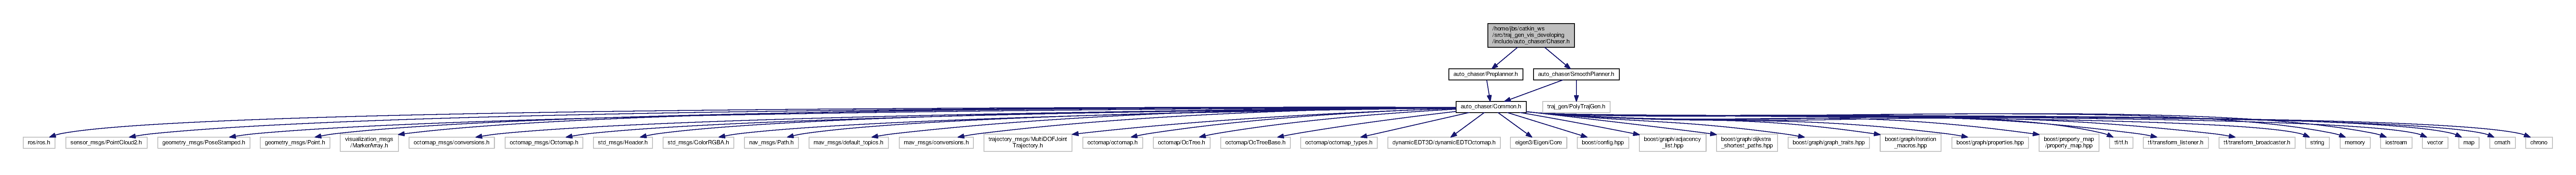
\includegraphics[width=350pt]{_chaser_8h__incl}
\end{center}
\end{figure}
This graph shows which files directly or indirectly include this file\+:
\nopagebreak
\begin{figure}[H]
\begin{center}
\leavevmode
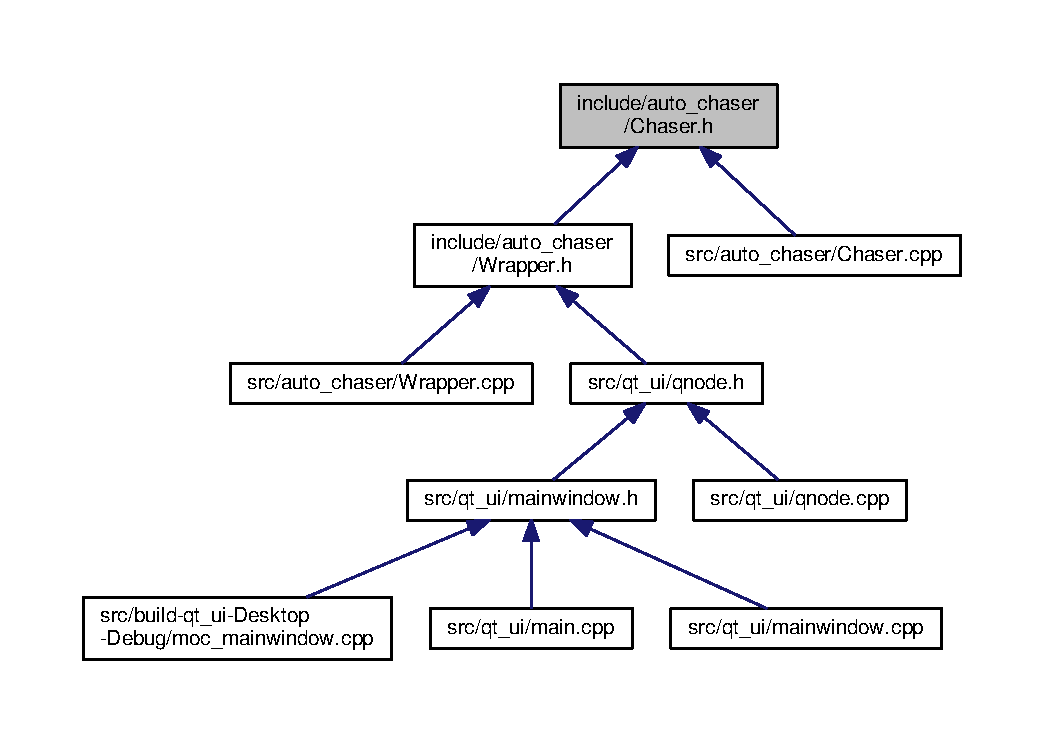
\includegraphics[width=350pt]{_chaser_8h__dep__incl}
\end{center}
\end{figure}
\subsection*{Classes}
\begin{DoxyCompactItemize}
\item 
class \hyperlink{class_chaser}{Chaser}
\end{DoxyCompactItemize}

\hypertarget{_common_8h}{}\section{include/auto\+\_\+chaser/\+Common.h File Reference}
\label{_common_8h}\index{include/auto\+\_\+chaser/\+Common.\+h@{include/auto\+\_\+chaser/\+Common.\+h}}
{\ttfamily \#include $<$ros/ros.\+h$>$}\\*
{\ttfamily \#include $<$sensor\+\_\+msgs/\+Point\+Cloud2.\+h$>$}\\*
{\ttfamily \#include $<$geometry\+\_\+msgs/\+Pose\+Stamped.\+h$>$}\\*
{\ttfamily \#include $<$geometry\+\_\+msgs/\+Point.\+h$>$}\\*
{\ttfamily \#include $<$visualization\+\_\+msgs/\+Marker\+Array.\+h$>$}\\*
{\ttfamily \#include $<$octomap\+\_\+msgs/conversions.\+h$>$}\\*
{\ttfamily \#include $<$octomap\+\_\+msgs/\+Octomap.\+h$>$}\\*
{\ttfamily \#include $<$std\+\_\+msgs/\+Header.\+h$>$}\\*
{\ttfamily \#include $<$std\+\_\+msgs/\+Color\+R\+G\+B\+A.\+h$>$}\\*
{\ttfamily \#include $<$nav\+\_\+msgs/\+Path.\+h$>$}\\*
{\ttfamily \#include $<$octomap/octomap.\+h$>$}\\*
{\ttfamily \#include $<$octomap/\+Oc\+Tree.\+h$>$}\\*
{\ttfamily \#include $<$octomap/\+Oc\+Tree\+Base.\+h$>$}\\*
{\ttfamily \#include $<$octomap/octomap\+\_\+types.\+h$>$}\\*
{\ttfamily \#include $<$dynamic\+E\+D\+T3\+D/dynamic\+E\+D\+T\+Octomap.\+h$>$}\\*
{\ttfamily \#include $<$eigen3/\+Eigen/\+Core$>$}\\*
{\ttfamily \#include $<$boost/config.\+hpp$>$}\\*
{\ttfamily \#include $<$boost/graph/adjacency\+\_\+list.\+hpp$>$}\\*
{\ttfamily \#include $<$boost/graph/dijkstra\+\_\+shortest\+\_\+paths.\+hpp$>$}\\*
{\ttfamily \#include $<$boost/graph/graph\+\_\+traits.\+hpp$>$}\\*
{\ttfamily \#include $<$boost/graph/iteration\+\_\+macros.\+hpp$>$}\\*
{\ttfamily \#include $<$boost/graph/properties.\+hpp$>$}\\*
{\ttfamily \#include $<$boost/property\+\_\+map/property\+\_\+map.\+hpp$>$}\\*
{\ttfamily \#include $<$tf/tf.\+h$>$}\\*
{\ttfamily \#include $<$tf/transform\+\_\+listener.\+h$>$}\\*
{\ttfamily \#include $<$tf/transform\+\_\+broadcaster.\+h$>$}\\*
{\ttfamily \#include $<$string$>$}\\*
{\ttfamily \#include $<$memory$>$}\\*
{\ttfamily \#include $<$iostream$>$}\\*
{\ttfamily \#include $<$vector$>$}\\*
{\ttfamily \#include $<$map$>$}\\*
{\ttfamily \#include $<$cmath$>$}\\*
{\ttfamily \#include $<$chrono$>$}\\*
Include dependency graph for Common.\+h\+:
\nopagebreak
\begin{figure}[H]
\begin{center}
\leavevmode
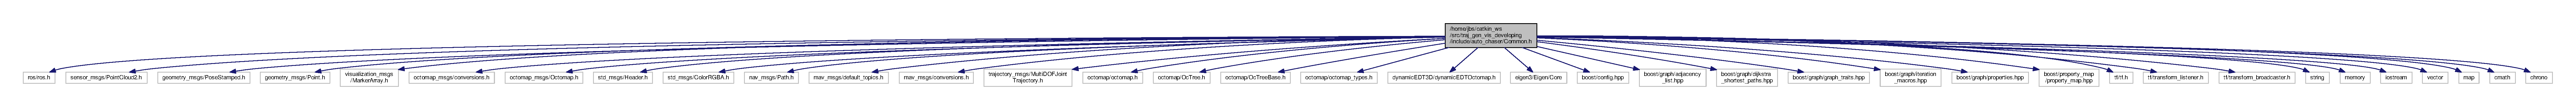
\includegraphics[width=350pt]{_common_8h__incl}
\end{center}
\end{figure}
This graph shows which files directly or indirectly include this file\+:
\nopagebreak
\begin{figure}[H]
\begin{center}
\leavevmode
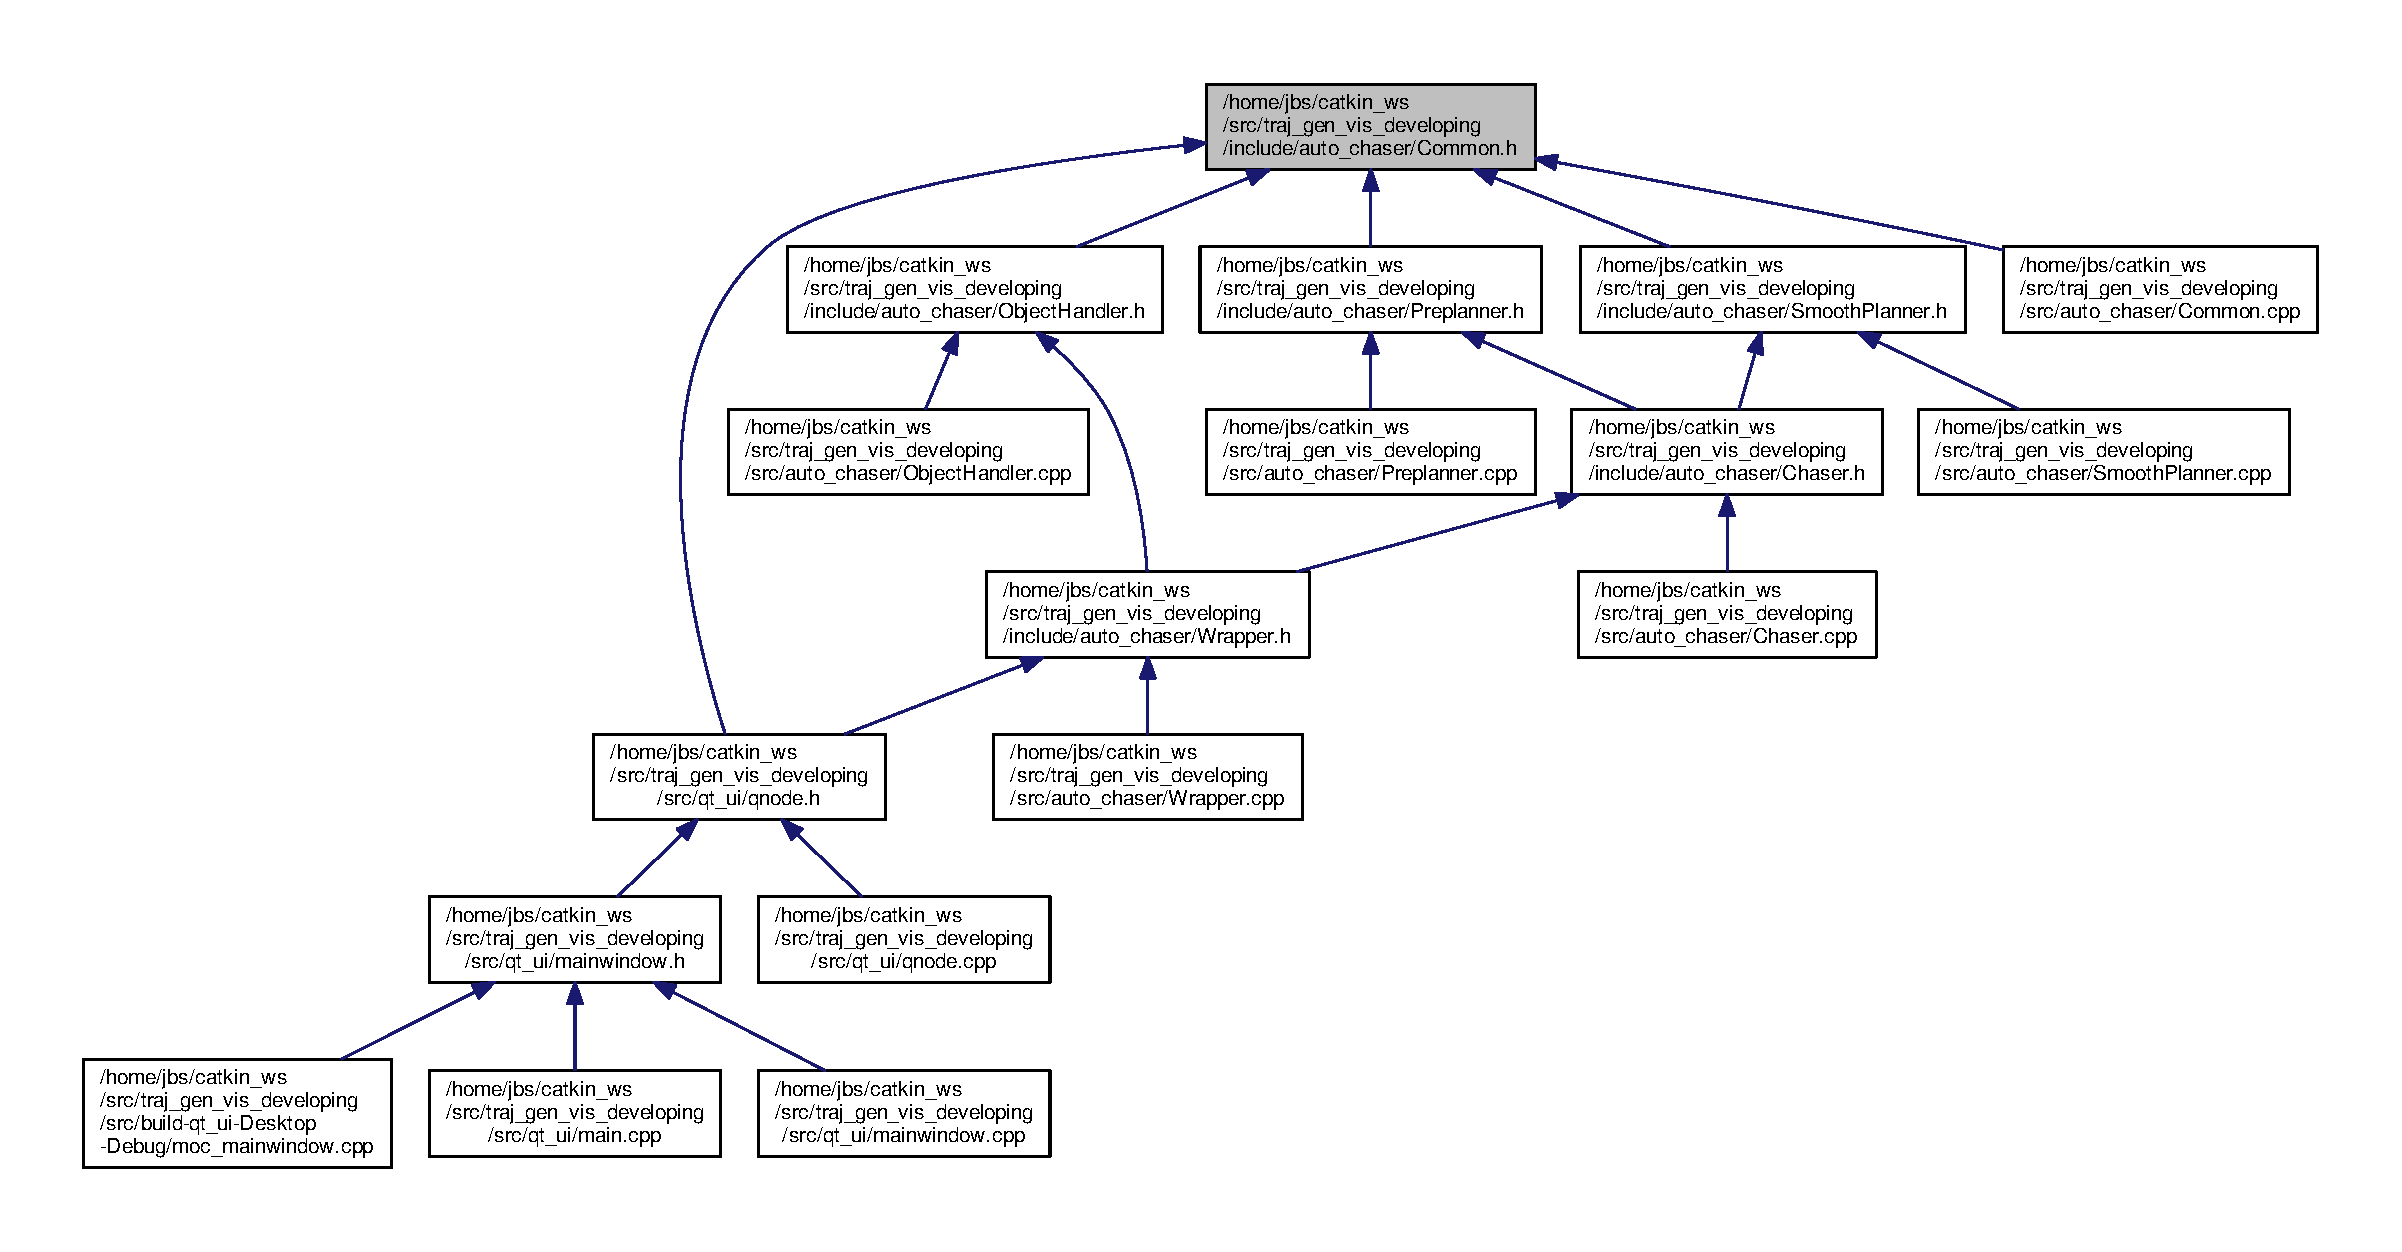
\includegraphics[width=350pt]{_common_8h__dep__incl}
\end{center}
\end{figure}
\subsection*{Classes}
\begin{DoxyCompactItemize}
\item 
struct \hyperlink{struct_node}{Node$<$ T $>$}
\item 
struct \hyperlink{struct_field_params}{Field\+Params}
\item 
struct \hyperlink{structchaser_1_1_preplanner_params}{chaser\+::\+Preplanner\+Params}
\item 
struct \hyperlink{structchaser_1_1_smoothplanner_params}{chaser\+::\+Smoothplanner\+Params}
\item 
struct \hyperlink{struct_grid_field}{Grid\+Field}
\end{DoxyCompactItemize}
\subsection*{Namespaces}
\begin{DoxyCompactItemize}
\item 
 \hyperlink{namespacechaser}{chaser}
\end{DoxyCompactItemize}
\subsection*{Macros}
\begin{DoxyCompactItemize}
\item 
\#define \hyperlink{_common_8h_af0c0d1034a71f8aa3a08cda83c9d4e7a}{Get\+Current\+Dir}~getcwd
\end{DoxyCompactItemize}
\subsection*{Typedefs}
\begin{DoxyCompactItemize}
\item 
typedef double \hyperlink{_common_8h_a5b53e5716aeadbb040a52c9c8c124c74}{Weight}
\item 
typedef boost\+::property$<$ boost\+::edge\+\_\+weight\+\_\+t, \hyperlink{_common_8h_a5b53e5716aeadbb040a52c9c8c124c74}{Weight} $>$ \hyperlink{_common_8h_adafd959ae5e10fee25f0d54353dc5714}{Weight\+Property}
\item 
typedef boost\+::property$<$ boost\+::vertex\+\_\+name\+\_\+t, Point $>$ \hyperlink{_common_8h_ae8aea6c699e4a47da0110059c52e94d1}{Name\+Property}
\item 
typedef boost\+::adjacency\+\_\+list$<$ boost\+::listS, boost\+::vecS, boost\+::directedS, \hyperlink{_common_8h_ae8aea6c699e4a47da0110059c52e94d1}{Name\+Property}, \hyperlink{_common_8h_adafd959ae5e10fee25f0d54353dc5714}{Weight\+Property} $>$ \hyperlink{_common_8h_a45f376d452c699e18013842e64602733}{Graph}
\item 
typedef boost\+::graph\+\_\+traits$<$ \hyperlink{_common_8h_a45f376d452c699e18013842e64602733}{Graph} $>$\+::vertex\+\_\+descriptor \hyperlink{_common_8h_a1f671d518f573b692b5efa57ed576f36}{Vertex\+\_\+d}
\item 
typedef string \hyperlink{_common_8h_a817e52d0171d1503034d4cbe7fd89a1b}{Vertex\+Name}
\item 
typedef boost\+::property\+\_\+map$<$ \hyperlink{_common_8h_a45f376d452c699e18013842e64602733}{Graph}, boost\+::vertex\+\_\+index\+\_\+t $>$\+::type \hyperlink{_common_8h_a7fb6309a04472de0c8cb8c74ebf92c5e}{Index\+Map}
\item 
typedef boost\+::property\+\_\+map$<$ \hyperlink{_common_8h_a45f376d452c699e18013842e64602733}{Graph}, boost\+::vertex\+\_\+name\+\_\+t $>$\+::type \hyperlink{_common_8h_a7a347729377841627777cbe0a6becbf9}{Name\+Map}
\item 
typedef boost\+::iterator\+\_\+property\+\_\+map$<$ \hyperlink{_common_8h_a1f671d518f573b692b5efa57ed576f36}{Vertex\+\_\+d} $\ast$, \hyperlink{_common_8h_a7fb6309a04472de0c8cb8c74ebf92c5e}{Index\+Map}, \hyperlink{_common_8h_a1f671d518f573b692b5efa57ed576f36}{Vertex\+\_\+d}, \hyperlink{_common_8h_a1f671d518f573b692b5efa57ed576f36}{Vertex\+\_\+d} \& $>$ \hyperlink{_common_8h_a3e372f12838999c89bb6fafe2c9b4363}{Predecessor\+Map}
\item 
typedef boost\+::iterator\+\_\+property\+\_\+map$<$ \hyperlink{_common_8h_a5b53e5716aeadbb040a52c9c8c124c74}{Weight} $\ast$, \hyperlink{_common_8h_a7fb6309a04472de0c8cb8c74ebf92c5e}{Index\+Map}, \hyperlink{_common_8h_a5b53e5716aeadbb040a52c9c8c124c74}{Weight}, \hyperlink{_common_8h_a5b53e5716aeadbb040a52c9c8c124c74}{Weight} \& $>$ \hyperlink{_common_8h_acab893c91ba1c4e4415b652ccebeea6a}{Distance\+Map}
\item 
typedef vector$<$ Point $>$ \hyperlink{_common_8h_a225da2de31d0161f43841ed31cac064c}{Vertex\+Path}
\item 
typedef map$<$ \hyperlink{_common_8h_a817e52d0171d1503034d4cbe7fd89a1b}{Vertex\+Name}, \hyperlink{_common_8h_a1f671d518f573b692b5efa57ed576f36}{Vertex\+\_\+d} $>$ \hyperlink{_common_8h_a25b10a034823d9ab576650719f0d331c}{Descriptor\+Map}
\end{DoxyCompactItemize}
\subsection*{Functions}
\begin{DoxyCompactItemize}
\item 
std\+::string \hyperlink{_common_8h_a7770cb36d4f4c6e78ff68516ecb2123c}{Get\+Current\+Working\+Dir} (void)
\item 
vector$<$ Point $>$ \hyperlink{_common_8h_a81915b091c29bc9aef6a74ab374f479a}{extract\+\_\+pnts\+\_\+from\+\_\+path} (nav\+\_\+msgs\+::\+Path)
\item 
Vector3f \hyperlink{_common_8h_a3e35de4eb7396984c2c5018768885d91}{geo2eigen} (const Point \&)
\item 
void \hyperlink{_common_8h_a75aaebf1a8b822524cc6af51a0cd83ef}{get\+\_\+color} (float x\+\_\+in, float \&r, float \&g, float \&b)
\item 
void \hyperlink{_common_8h_a4b2e4b6698ff92678b23392dc111b36d}{get\+\_\+color\+\_\+dist} (float dist\+\_\+val, std\+\_\+msgs\+::\+Color\+R\+G\+BA \&color, float max\+\_\+plot\+\_\+dist\+\_\+val)
\end{DoxyCompactItemize}


\subsection{Macro Definition Documentation}
\index{Common.\+h@{Common.\+h}!Get\+Current\+Dir@{Get\+Current\+Dir}}
\index{Get\+Current\+Dir@{Get\+Current\+Dir}!Common.\+h@{Common.\+h}}
\subsubsection[{\texorpdfstring{Get\+Current\+Dir}{GetCurrentDir}}]{\setlength{\rightskip}{0pt plus 5cm}\#define Get\+Current\+Dir~getcwd}\hypertarget{_common_8h_af0c0d1034a71f8aa3a08cda83c9d4e7a}{}\label{_common_8h_af0c0d1034a71f8aa3a08cda83c9d4e7a}


\subsection{Typedef Documentation}
\index{Common.\+h@{Common.\+h}!Descriptor\+Map@{Descriptor\+Map}}
\index{Descriptor\+Map@{Descriptor\+Map}!Common.\+h@{Common.\+h}}
\subsubsection[{\texorpdfstring{Descriptor\+Map}{DescriptorMap}}]{\setlength{\rightskip}{0pt plus 5cm}typedef map$<${\bf Vertex\+Name},{\bf Vertex\+\_\+d}$>$ {\bf Descriptor\+Map}}\hypertarget{_common_8h_a25b10a034823d9ab576650719f0d331c}{}\label{_common_8h_a25b10a034823d9ab576650719f0d331c}
\index{Common.\+h@{Common.\+h}!Distance\+Map@{Distance\+Map}}
\index{Distance\+Map@{Distance\+Map}!Common.\+h@{Common.\+h}}
\subsubsection[{\texorpdfstring{Distance\+Map}{DistanceMap}}]{\setlength{\rightskip}{0pt plus 5cm}typedef boost\+::iterator\+\_\+property\+\_\+map$<$ {\bf Weight}$\ast$, {\bf Index\+Map}, {\bf Weight}, {\bf Weight}\& $>$ {\bf Distance\+Map}}\hypertarget{_common_8h_acab893c91ba1c4e4415b652ccebeea6a}{}\label{_common_8h_acab893c91ba1c4e4415b652ccebeea6a}
\index{Common.\+h@{Common.\+h}!Graph@{Graph}}
\index{Graph@{Graph}!Common.\+h@{Common.\+h}}
\subsubsection[{\texorpdfstring{Graph}{Graph}}]{\setlength{\rightskip}{0pt plus 5cm}typedef boost\+::adjacency\+\_\+list$<$ boost\+::listS, boost\+::vecS, boost\+::directedS, {\bf Name\+Property}, {\bf Weight\+Property} $>$ {\bf Graph}}\hypertarget{_common_8h_a45f376d452c699e18013842e64602733}{}\label{_common_8h_a45f376d452c699e18013842e64602733}
\index{Common.\+h@{Common.\+h}!Index\+Map@{Index\+Map}}
\index{Index\+Map@{Index\+Map}!Common.\+h@{Common.\+h}}
\subsubsection[{\texorpdfstring{Index\+Map}{IndexMap}}]{\setlength{\rightskip}{0pt plus 5cm}typedef boost\+::property\+\_\+map$<$ {\bf Graph}, boost\+::vertex\+\_\+index\+\_\+t $>$\+::type {\bf Index\+Map}}\hypertarget{_common_8h_a7fb6309a04472de0c8cb8c74ebf92c5e}{}\label{_common_8h_a7fb6309a04472de0c8cb8c74ebf92c5e}
\index{Common.\+h@{Common.\+h}!Name\+Map@{Name\+Map}}
\index{Name\+Map@{Name\+Map}!Common.\+h@{Common.\+h}}
\subsubsection[{\texorpdfstring{Name\+Map}{NameMap}}]{\setlength{\rightskip}{0pt plus 5cm}typedef boost\+::property\+\_\+map$<$ {\bf Graph}, boost\+::vertex\+\_\+name\+\_\+t $>$\+::type {\bf Name\+Map}}\hypertarget{_common_8h_a7a347729377841627777cbe0a6becbf9}{}\label{_common_8h_a7a347729377841627777cbe0a6becbf9}
\index{Common.\+h@{Common.\+h}!Name\+Property@{Name\+Property}}
\index{Name\+Property@{Name\+Property}!Common.\+h@{Common.\+h}}
\subsubsection[{\texorpdfstring{Name\+Property}{NameProperty}}]{\setlength{\rightskip}{0pt plus 5cm}typedef boost\+::property$<$boost\+::vertex\+\_\+name\+\_\+t, Point$>$ {\bf Name\+Property}}\hypertarget{_common_8h_ae8aea6c699e4a47da0110059c52e94d1}{}\label{_common_8h_ae8aea6c699e4a47da0110059c52e94d1}
\index{Common.\+h@{Common.\+h}!Predecessor\+Map@{Predecessor\+Map}}
\index{Predecessor\+Map@{Predecessor\+Map}!Common.\+h@{Common.\+h}}
\subsubsection[{\texorpdfstring{Predecessor\+Map}{PredecessorMap}}]{\setlength{\rightskip}{0pt plus 5cm}typedef boost\+::iterator\+\_\+property\+\_\+map$<$ {\bf Vertex\+\_\+d}$\ast$, {\bf Index\+Map}, {\bf Vertex\+\_\+d}, {\bf Vertex\+\_\+d}\& $>$ {\bf Predecessor\+Map}}\hypertarget{_common_8h_a3e372f12838999c89bb6fafe2c9b4363}{}\label{_common_8h_a3e372f12838999c89bb6fafe2c9b4363}
\index{Common.\+h@{Common.\+h}!Vertex\+\_\+d@{Vertex\+\_\+d}}
\index{Vertex\+\_\+d@{Vertex\+\_\+d}!Common.\+h@{Common.\+h}}
\subsubsection[{\texorpdfstring{Vertex\+\_\+d}{Vertex_d}}]{\setlength{\rightskip}{0pt plus 5cm}typedef boost\+::graph\+\_\+traits$<$ {\bf Graph} $>$\+::vertex\+\_\+descriptor {\bf Vertex\+\_\+d}}\hypertarget{_common_8h_a1f671d518f573b692b5efa57ed576f36}{}\label{_common_8h_a1f671d518f573b692b5efa57ed576f36}
\index{Common.\+h@{Common.\+h}!Vertex\+Name@{Vertex\+Name}}
\index{Vertex\+Name@{Vertex\+Name}!Common.\+h@{Common.\+h}}
\subsubsection[{\texorpdfstring{Vertex\+Name}{VertexName}}]{\setlength{\rightskip}{0pt plus 5cm}typedef string {\bf Vertex\+Name}}\hypertarget{_common_8h_a817e52d0171d1503034d4cbe7fd89a1b}{}\label{_common_8h_a817e52d0171d1503034d4cbe7fd89a1b}
\index{Common.\+h@{Common.\+h}!Vertex\+Path@{Vertex\+Path}}
\index{Vertex\+Path@{Vertex\+Path}!Common.\+h@{Common.\+h}}
\subsubsection[{\texorpdfstring{Vertex\+Path}{VertexPath}}]{\setlength{\rightskip}{0pt plus 5cm}typedef vector$<$Point$>$ {\bf Vertex\+Path}}\hypertarget{_common_8h_a225da2de31d0161f43841ed31cac064c}{}\label{_common_8h_a225da2de31d0161f43841ed31cac064c}
\index{Common.\+h@{Common.\+h}!Weight@{Weight}}
\index{Weight@{Weight}!Common.\+h@{Common.\+h}}
\subsubsection[{\texorpdfstring{Weight}{Weight}}]{\setlength{\rightskip}{0pt plus 5cm}typedef double {\bf Weight}}\hypertarget{_common_8h_a5b53e5716aeadbb040a52c9c8c124c74}{}\label{_common_8h_a5b53e5716aeadbb040a52c9c8c124c74}
Boost graph library \index{Common.\+h@{Common.\+h}!Weight\+Property@{Weight\+Property}}
\index{Weight\+Property@{Weight\+Property}!Common.\+h@{Common.\+h}}
\subsubsection[{\texorpdfstring{Weight\+Property}{WeightProperty}}]{\setlength{\rightskip}{0pt plus 5cm}typedef boost\+::property$<$boost\+::edge\+\_\+weight\+\_\+t, {\bf Weight}$>$ {\bf Weight\+Property}}\hypertarget{_common_8h_adafd959ae5e10fee25f0d54353dc5714}{}\label{_common_8h_adafd959ae5e10fee25f0d54353dc5714}


\subsection{Function Documentation}
\index{Common.\+h@{Common.\+h}!extract\+\_\+pnts\+\_\+from\+\_\+path@{extract\+\_\+pnts\+\_\+from\+\_\+path}}
\index{extract\+\_\+pnts\+\_\+from\+\_\+path@{extract\+\_\+pnts\+\_\+from\+\_\+path}!Common.\+h@{Common.\+h}}
\subsubsection[{\texorpdfstring{extract\+\_\+pnts\+\_\+from\+\_\+path(nav\+\_\+msgs\+::\+Path)}{extract_pnts_from_path(nav_msgs::Path)}}]{\setlength{\rightskip}{0pt plus 5cm}vector$<$Point$>$ extract\+\_\+pnts\+\_\+from\+\_\+path (
\begin{DoxyParamCaption}
\item[{nav\+\_\+msgs\+::\+Path}]{}
\end{DoxyParamCaption}
)}\hypertarget{_common_8h_a81915b091c29bc9aef6a74ab374f479a}{}\label{_common_8h_a81915b091c29bc9aef6a74ab374f479a}
Functions 
\begin{DoxyCode}
10                                                        \{
11 
12   vector<Point> pnt\_seq;
13   \textcolor{keywordflow}{for}(\textcolor{keyword}{auto} it = path.poses.begin(); it<path.poses.end();it++)\{
14     pnt\_seq.push\_back(it->pose.position);
15   \}
16   \textcolor{keywordflow}{return} pnt\_seq;
17 \};
\end{DoxyCode}
\index{Common.\+h@{Common.\+h}!geo2eigen@{geo2eigen}}
\index{geo2eigen@{geo2eigen}!Common.\+h@{Common.\+h}}
\subsubsection[{\texorpdfstring{geo2eigen(const Point \&)}{geo2eigen(const Point &)}}]{\setlength{\rightskip}{0pt plus 5cm}Vector3f geo2eigen (
\begin{DoxyParamCaption}
\item[{const Point \&}]{}
\end{DoxyParamCaption}
)}\hypertarget{_common_8h_a3e35de4eb7396984c2c5018768885d91}{}\label{_common_8h_a3e35de4eb7396984c2c5018768885d91}

\begin{DoxyCode}
19                                     \{
20 
21   \textcolor{keywordflow}{return} Vector3f(pnt.x,pnt.y,pnt.z);
22 \};
\end{DoxyCode}
\index{Common.\+h@{Common.\+h}!get\+\_\+color@{get\+\_\+color}}
\index{get\+\_\+color@{get\+\_\+color}!Common.\+h@{Common.\+h}}
\subsubsection[{\texorpdfstring{get\+\_\+color(float x\+\_\+in, float \&r, float \&g, float \&b)}{get_color(float x_in, float &r, float &g, float &b)}}]{\setlength{\rightskip}{0pt plus 5cm}void get\+\_\+color (
\begin{DoxyParamCaption}
\item[{float}]{x\+\_\+in, }
\item[{float \&}]{r, }
\item[{float \&}]{g, }
\item[{float \&}]{b}
\end{DoxyParamCaption}
)}\hypertarget{_common_8h_a75aaebf1a8b822524cc6af51a0cd83ef}{}\label{_common_8h_a75aaebf1a8b822524cc6af51a0cd83ef}

\begin{DoxyCode}
51 \{
52   \textcolor{comment}{// Only important if the number of colors is small. In which case the rest is}
53   \textcolor{comment}{// still wrong anyway}
54   \textcolor{comment}{// x = linspace(0,1,jj)' * (1-1/jj) + 1/jj;}
55   \textcolor{comment}{//}
56   \textcolor{keyword}{const} \textcolor{keywordtype}{double} rone = 0.8;
57   \textcolor{keyword}{const} \textcolor{keywordtype}{double} gone = 1.0;
58   \textcolor{keyword}{const} \textcolor{keywordtype}{double} bone = 1.0;
59   \textcolor{keywordtype}{float} x = x\_in;
60   x = (x\_in<0 ? 0 : (x>1 ? 1 : x));
61 
62   \textcolor{keywordflow}{if} (x<1. / 8.)
63   \{
64     r = 0;
65     g = 0;
66     b = bone*(0.5 + (x) / (1. / 8.)*0.5);
67   \} \textcolor{keywordflow}{else} \textcolor{keywordflow}{if} (x<3. / 8.)
68   \{
69     r = 0;
70     g = gone*(x - 1. / 8.) / (3. / 8. - 1. / 8.);
71     b = bone;
72   \} \textcolor{keywordflow}{else} \textcolor{keywordflow}{if} (x<5. / 8.)
73   \{
74     r = rone*(x - 3. / 8.) / (5. / 8. - 3. / 8.);
75     g = gone;
76     b = (bone - (x - 3. / 8.) / (5. / 8. - 3. / 8.));
77   \} \textcolor{keywordflow}{else} \textcolor{keywordflow}{if} (x<7. / 8.)
78   \{
79     r = rone;
80     g = (gone - (x - 5. / 8.) / (7. / 8. - 5. / 8.));
81     b = 0;
82   \} \textcolor{keywordflow}{else}
83   \{
84     r = (rone - (x - 7. / 8.) / (1. - 7. / 8.)*0.5);
85     g = 0;
86     b = 0;
87   \}
88 \}
\end{DoxyCode}
\index{Common.\+h@{Common.\+h}!get\+\_\+color\+\_\+dist@{get\+\_\+color\+\_\+dist}}
\index{get\+\_\+color\+\_\+dist@{get\+\_\+color\+\_\+dist}!Common.\+h@{Common.\+h}}
\subsubsection[{\texorpdfstring{get\+\_\+color\+\_\+dist(float dist\+\_\+val, std\+\_\+msgs\+::\+Color\+R\+G\+B\+A \&color, float max\+\_\+plot\+\_\+dist\+\_\+val)}{get_color_dist(float dist_val, std_msgs::ColorRGBA &color, float max_plot_dist_val)}}]{\setlength{\rightskip}{0pt plus 5cm}void get\+\_\+color\+\_\+dist (
\begin{DoxyParamCaption}
\item[{float}]{dist\+\_\+val, }
\item[{std\+\_\+msgs\+::\+Color\+R\+G\+BA \&}]{color, }
\item[{float}]{max\+\_\+plot\+\_\+dist\+\_\+val}
\end{DoxyParamCaption}
)}\hypertarget{_common_8h_a4b2e4b6698ff92678b23392dc111b36d}{}\label{_common_8h_a4b2e4b6698ff92678b23392dc111b36d}

\begin{DoxyCode}
25                                                                                      \{
26 \textcolor{comment}{// error region }
27   \textcolor{keywordflow}{if}(dist\_val<0)\{
28       color.r = 0.5;
29       color.g = 0.0;
30       color.b = 0.0;
31       color.a = 0.2;
32 
33   \}
34 \textcolor{comment}{//   else if(dist\_val == 0.2)\{}
35 \textcolor{comment}{//       color.r = 0;}
36 \textcolor{comment}{//       color.g = 0;}
37 \textcolor{comment}{//       color.b = 1;}
38 \textcolor{comment}{//   \}}
39   \textcolor{comment}{// normal region }
40   \textcolor{keywordflow}{else}\{                   
41       color.r = pow(dist\_val/max\_plot\_dist\_val,3);
42       color.g = pow(dist\_val/max\_plot\_dist\_val,3);
43       color.b = pow(dist\_val/max\_plot\_dist\_val,3);
44   \}
45   \textcolor{comment}{// plot only cells in this bound}
46   \textcolor{keywordflow}{if}(dist\_val<max\_plot\_dist\_val)
47       color.a = 0.2;
48 \};
\end{DoxyCode}
\index{Common.\+h@{Common.\+h}!Get\+Current\+Working\+Dir@{Get\+Current\+Working\+Dir}}
\index{Get\+Current\+Working\+Dir@{Get\+Current\+Working\+Dir}!Common.\+h@{Common.\+h}}
\subsubsection[{\texorpdfstring{Get\+Current\+Working\+Dir(void)}{GetCurrentWorkingDir(void)}}]{\setlength{\rightskip}{0pt plus 5cm}std\+::string Get\+Current\+Working\+Dir (
\begin{DoxyParamCaption}
\item[{void}]{}
\end{DoxyParamCaption}
)}\hypertarget{_common_8h_a7770cb36d4f4c6e78ff68516ecb2123c}{}\label{_common_8h_a7770cb36d4f4c6e78ff68516ecb2123c}

\begin{DoxyCode}
2                                       \{
3     \textcolor{keywordtype}{char} buff[FILENAME\_MAX];
4     \hyperlink{_common_8h_af0c0d1034a71f8aa3a08cda83c9d4e7a}{GetCurrentDir}( buff, FILENAME\_MAX );
5     std::string current\_working\_dir(buff);
6     \textcolor{keywordflow}{return} current\_working\_dir; 
7 \}
\end{DoxyCode}

\hypertarget{_evaluator_8h}{}\section{/home/jbs/catkin\+\_\+ws/src/traj\+\_\+gen\+\_\+vis\+\_\+developing/include/auto\+\_\+chaser/\+Evaluator.h File Reference}
\label{_evaluator_8h}\index{/home/jbs/catkin\+\_\+ws/src/traj\+\_\+gen\+\_\+vis\+\_\+developing/include/auto\+\_\+chaser/\+Evaluator.\+h@{/home/jbs/catkin\+\_\+ws/src/traj\+\_\+gen\+\_\+vis\+\_\+developing/include/auto\+\_\+chaser/\+Evaluator.\+h}}

\hypertarget{_object_handler_8h}{}\section{/home/jbs/catkin\+\_\+ws/src/traj\+\_\+gen\+\_\+vis\+\_\+developing/include/auto\+\_\+chaser/\+Object\+Handler.h File Reference}
\label{_object_handler_8h}\index{/home/jbs/catkin\+\_\+ws/src/traj\+\_\+gen\+\_\+vis\+\_\+developing/include/auto\+\_\+chaser/\+Object\+Handler.\+h@{/home/jbs/catkin\+\_\+ws/src/traj\+\_\+gen\+\_\+vis\+\_\+developing/include/auto\+\_\+chaser/\+Object\+Handler.\+h}}
{\ttfamily \#include \char`\"{}auto\+\_\+chaser/\+Common.\+h\char`\"{}}\\*
Include dependency graph for Object\+Handler.\+h\+:
\nopagebreak
\begin{figure}[H]
\begin{center}
\leavevmode
\includegraphics[width=350pt]{_object_handler_8h__incl}
\end{center}
\end{figure}
This graph shows which files directly or indirectly include this file\+:
\nopagebreak
\begin{figure}[H]
\begin{center}
\leavevmode
\includegraphics[width=350pt]{_object_handler_8h__dep__incl}
\end{center}
\end{figure}
\subsection*{Classes}
\begin{DoxyCompactItemize}
\item 
class \hyperlink{class_objects_handler}{Objects\+Handler}
\end{DoxyCompactItemize}

\hypertarget{_preplanner_8h}{}\section{/home/jbs/catkin\+\_\+ws/src/traj\+\_\+gen\+\_\+vis\+\_\+developing/include/auto\+\_\+chaser/\+Preplanner.h File Reference}
\label{_preplanner_8h}\index{/home/jbs/catkin\+\_\+ws/src/traj\+\_\+gen\+\_\+vis\+\_\+developing/include/auto\+\_\+chaser/\+Preplanner.\+h@{/home/jbs/catkin\+\_\+ws/src/traj\+\_\+gen\+\_\+vis\+\_\+developing/include/auto\+\_\+chaser/\+Preplanner.\+h}}
{\ttfamily \#include \char`\"{}auto\+\_\+chaser/\+Common.\+h\char`\"{}}\\*
Include dependency graph for Preplanner.\+h\+:
\nopagebreak
\begin{figure}[H]
\begin{center}
\leavevmode
\includegraphics[width=350pt]{_preplanner_8h__incl}
\end{center}
\end{figure}
This graph shows which files directly or indirectly include this file\+:
\nopagebreak
\begin{figure}[H]
\begin{center}
\leavevmode
\includegraphics[width=350pt]{_preplanner_8h__dep__incl}
\end{center}
\end{figure}
\subsection*{Classes}
\begin{DoxyCompactItemize}
\item 
class \hyperlink{class_preplanner}{Preplanner}
\end{DoxyCompactItemize}

\hypertarget{_smooth_planner_8h}{}\section{include/auto\+\_\+chaser/\+Smooth\+Planner.h File Reference}
\label{_smooth_planner_8h}\index{include/auto\+\_\+chaser/\+Smooth\+Planner.\+h@{include/auto\+\_\+chaser/\+Smooth\+Planner.\+h}}
{\ttfamily \#include \char`\"{}auto\+\_\+chaser/\+Common.\+h\char`\"{}}\\*
{\ttfamily \#include \char`\"{}traj\+\_\+gen/\+Poly\+Traj\+Gen.\+h\char`\"{}}\\*
Include dependency graph for Smooth\+Planner.\+h\+:
\nopagebreak
\begin{figure}[H]
\begin{center}
\leavevmode
\includegraphics[width=350pt]{_smooth_planner_8h__incl}
\end{center}
\end{figure}
This graph shows which files directly or indirectly include this file\+:
\nopagebreak
\begin{figure}[H]
\begin{center}
\leavevmode
\includegraphics[width=350pt]{_smooth_planner_8h__dep__incl}
\end{center}
\end{figure}
\subsection*{Classes}
\begin{DoxyCompactItemize}
\item 
class \hyperlink{class_smooth_planner}{Smooth\+Planner}
\end{DoxyCompactItemize}

\hypertarget{_wrapper_8h}{}\section{/home/jbs/catkin\+\_\+ws/src/traj\+\_\+gen\+\_\+vis\+\_\+developing/include/auto\+\_\+chaser/\+Wrapper.h File Reference}
\label{_wrapper_8h}\index{/home/jbs/catkin\+\_\+ws/src/traj\+\_\+gen\+\_\+vis\+\_\+developing/include/auto\+\_\+chaser/\+Wrapper.\+h@{/home/jbs/catkin\+\_\+ws/src/traj\+\_\+gen\+\_\+vis\+\_\+developing/include/auto\+\_\+chaser/\+Wrapper.\+h}}
{\ttfamily \#include \char`\"{}auto\+\_\+chaser/\+Chaser.\+h\char`\"{}}\\*
{\ttfamily \#include \char`\"{}auto\+\_\+chaser/\+Object\+Handler.\+h\char`\"{}}\\*
Include dependency graph for Wrapper.\+h\+:
\nopagebreak
\begin{figure}[H]
\begin{center}
\leavevmode
\includegraphics[width=350pt]{_wrapper_8h__incl}
\end{center}
\end{figure}
This graph shows which files directly or indirectly include this file\+:
\nopagebreak
\begin{figure}[H]
\begin{center}
\leavevmode
\includegraphics[width=350pt]{_wrapper_8h__dep__incl}
\end{center}
\end{figure}
\subsection*{Classes}
\begin{DoxyCompactItemize}
\item 
class \hyperlink{class_wrapper}{Wrapper}
\end{DoxyCompactItemize}

\hypertarget{_target_manager_8h}{}\section{include/target\+\_\+manager/\+Target\+Manager.h File Reference}
\label{_target_manager_8h}\index{include/target\+\_\+manager/\+Target\+Manager.\+h@{include/target\+\_\+manager/\+Target\+Manager.\+h}}
{\ttfamily \#include \char`\"{}traj\+\_\+gen/\+Poly\+Traj\+Gen.\+h\char`\"{}}\\*
{\ttfamily \#include \char`\"{}chomp\+\_\+predict/chomp\+\_\+predict.\+h\char`\"{}}\\*
{\ttfamily \#include $<$tf/transform\+\_\+broadcaster.\+h$>$}\\*
Include dependency graph for Target\+Manager.\+h\+:
\nopagebreak
\begin{figure}[H]
\begin{center}
\leavevmode
\includegraphics[width=350pt]{_target_manager_8h__incl}
\end{center}
\end{figure}
This graph shows which files directly or indirectly include this file\+:
\nopagebreak
\begin{figure}[H]
\begin{center}
\leavevmode
\includegraphics[width=350pt]{_target_manager_8h__dep__incl}
\end{center}
\end{figure}
\subsection*{Classes}
\begin{DoxyCompactItemize}
\item 
class \hyperlink{class_target_manager}{Target\+Manager}
\begin{DoxyCompactList}\small\item\em Target manager to be used in no-\/prediction mode (prior target path is precomputed before simulation) \end{DoxyCompactList}\item 
class \hyperlink{class_target_predictor}{Target\+Predictor}
\begin{DoxyCompactList}\small\item\em Target predictor in prediction mode. \end{DoxyCompactList}\end{DoxyCompactItemize}

\hypertarget{_r_e_a_d_m_e_8md}{}\section{R\+E\+A\+D\+M\+E.\+md File Reference}
\label{_r_e_a_d_m_e_8md}\index{R\+E\+A\+D\+M\+E.\+md@{R\+E\+A\+D\+M\+E.\+md}}

\hypertarget{_chaser_8cpp}{}\section{/home/jbs/catkin\+\_\+ws/src/traj\+\_\+gen\+\_\+vis\+\_\+developing/src/auto\+\_\+chaser/\+Chaser.cpp File Reference}
\label{_chaser_8cpp}\index{/home/jbs/catkin\+\_\+ws/src/traj\+\_\+gen\+\_\+vis\+\_\+developing/src/auto\+\_\+chaser/\+Chaser.\+cpp@{/home/jbs/catkin\+\_\+ws/src/traj\+\_\+gen\+\_\+vis\+\_\+developing/src/auto\+\_\+chaser/\+Chaser.\+cpp}}
{\ttfamily \#include \char`\"{}auto\+\_\+chaser/\+Chaser.\+h\char`\"{}}\\*
Include dependency graph for Chaser.\+cpp\+:
\nopagebreak
\begin{figure}[H]
\begin{center}
\leavevmode
\includegraphics[width=350pt]{_chaser_8cpp__incl}
\end{center}
\end{figure}

\hypertarget{_common_8cpp}{}\section{src/auto\+\_\+chaser/\+Common.cpp File Reference}
\label{_common_8cpp}\index{src/auto\+\_\+chaser/\+Common.\+cpp@{src/auto\+\_\+chaser/\+Common.\+cpp}}
{\ttfamily \#include \char`\"{}auto\+\_\+chaser/\+Common.\+h\char`\"{}}\\*
Include dependency graph for Common.\+cpp\+:
\nopagebreak
\begin{figure}[H]
\begin{center}
\leavevmode
\includegraphics[width=350pt]{_common_8cpp__incl}
\end{center}
\end{figure}
\subsection*{Functions}
\begin{DoxyCompactItemize}
\item 
std\+::string \hyperlink{_common_8cpp_a7770cb36d4f4c6e78ff68516ecb2123c}{Get\+Current\+Working\+Dir} (void)
\item 
vector$<$ Point $>$ \hyperlink{_common_8cpp_a50cd37bbde872deb08960a0ee2748930}{extract\+\_\+pnts\+\_\+from\+\_\+path} (nav\+\_\+msgs\+::\+Path path)
\item 
Vector3f \hyperlink{_common_8cpp_af9dea61790454c1bd71a4472c099a778}{geo2eigen} (const Point \&pnt)
\item 
void \hyperlink{_common_8cpp_a4b2e4b6698ff92678b23392dc111b36d}{get\+\_\+color\+\_\+dist} (float dist\+\_\+val, std\+\_\+msgs\+::\+Color\+R\+G\+BA \&color, float max\+\_\+plot\+\_\+dist\+\_\+val)
\item 
void \hyperlink{_common_8cpp_a75aaebf1a8b822524cc6af51a0cd83ef}{get\+\_\+color} (float x\+\_\+in, float \&r, float \&g, float \&b)
\end{DoxyCompactItemize}


\subsection{Function Documentation}
\index{Common.\+cpp@{Common.\+cpp}!extract\+\_\+pnts\+\_\+from\+\_\+path@{extract\+\_\+pnts\+\_\+from\+\_\+path}}
\index{extract\+\_\+pnts\+\_\+from\+\_\+path@{extract\+\_\+pnts\+\_\+from\+\_\+path}!Common.\+cpp@{Common.\+cpp}}
\subsubsection[{\texorpdfstring{extract\+\_\+pnts\+\_\+from\+\_\+path(nav\+\_\+msgs\+::\+Path path)}{extract_pnts_from_path(nav_msgs::Path path)}}]{\setlength{\rightskip}{0pt plus 5cm}vector$<$Point$>$ extract\+\_\+pnts\+\_\+from\+\_\+path (
\begin{DoxyParamCaption}
\item[{nav\+\_\+msgs\+::\+Path}]{}
\end{DoxyParamCaption}
)}\hypertarget{_common_8cpp_a50cd37bbde872deb08960a0ee2748930}{}\label{_common_8cpp_a50cd37bbde872deb08960a0ee2748930}
Functions 
\begin{DoxyCode}
10                                                        \{
11 
12   vector<Point> pnt\_seq;
13   \textcolor{keywordflow}{for}(\textcolor{keyword}{auto} it = path.poses.begin(); it<path.poses.end();it++)\{
14     pnt\_seq.push\_back(it->pose.position);
15   \}
16   \textcolor{keywordflow}{return} pnt\_seq;
17 \};
\end{DoxyCode}
\index{Common.\+cpp@{Common.\+cpp}!geo2eigen@{geo2eigen}}
\index{geo2eigen@{geo2eigen}!Common.\+cpp@{Common.\+cpp}}
\subsubsection[{\texorpdfstring{geo2eigen(const Point \&pnt)}{geo2eigen(const Point &pnt)}}]{\setlength{\rightskip}{0pt plus 5cm}Vector3f geo2eigen (
\begin{DoxyParamCaption}
\item[{const Point \&}]{pnt}
\end{DoxyParamCaption}
)}\hypertarget{_common_8cpp_af9dea61790454c1bd71a4472c099a778}{}\label{_common_8cpp_af9dea61790454c1bd71a4472c099a778}

\begin{DoxyCode}
19                                     \{
20 
21   \textcolor{keywordflow}{return} Vector3f(pnt.x,pnt.y,pnt.z);
22 \};
\end{DoxyCode}
\index{Common.\+cpp@{Common.\+cpp}!get\+\_\+color@{get\+\_\+color}}
\index{get\+\_\+color@{get\+\_\+color}!Common.\+cpp@{Common.\+cpp}}
\subsubsection[{\texorpdfstring{get\+\_\+color(float x\+\_\+in, float \&r, float \&g, float \&b)}{get_color(float x_in, float &r, float &g, float &b)}}]{\setlength{\rightskip}{0pt plus 5cm}void get\+\_\+color (
\begin{DoxyParamCaption}
\item[{float}]{x\+\_\+in, }
\item[{float \&}]{r, }
\item[{float \&}]{g, }
\item[{float \&}]{b}
\end{DoxyParamCaption}
)}\hypertarget{_common_8cpp_a75aaebf1a8b822524cc6af51a0cd83ef}{}\label{_common_8cpp_a75aaebf1a8b822524cc6af51a0cd83ef}

\begin{DoxyCode}
51 \{
52   \textcolor{comment}{// Only important if the number of colors is small. In which case the rest is}
53   \textcolor{comment}{// still wrong anyway}
54   \textcolor{comment}{// x = linspace(0,1,jj)' * (1-1/jj) + 1/jj;}
55   \textcolor{comment}{//}
56   \textcolor{keyword}{const} \textcolor{keywordtype}{double} rone = 0.8;
57   \textcolor{keyword}{const} \textcolor{keywordtype}{double} gone = 1.0;
58   \textcolor{keyword}{const} \textcolor{keywordtype}{double} bone = 1.0;
59   \textcolor{keywordtype}{float} x = x\_in;
60   x = (x\_in<0 ? 0 : (x>1 ? 1 : x));
61 
62   \textcolor{keywordflow}{if} (x<1. / 8.)
63   \{
64     r = 0;
65     g = 0;
66     b = bone*(0.5 + (x) / (1. / 8.)*0.5);
67   \} \textcolor{keywordflow}{else} \textcolor{keywordflow}{if} (x<3. / 8.)
68   \{
69     r = 0;
70     g = gone*(x - 1. / 8.) / (3. / 8. - 1. / 8.);
71     b = bone;
72   \} \textcolor{keywordflow}{else} \textcolor{keywordflow}{if} (x<5. / 8.)
73   \{
74     r = rone*(x - 3. / 8.) / (5. / 8. - 3. / 8.);
75     g = gone;
76     b = (bone - (x - 3. / 8.) / (5. / 8. - 3. / 8.));
77   \} \textcolor{keywordflow}{else} \textcolor{keywordflow}{if} (x<7. / 8.)
78   \{
79     r = rone;
80     g = (gone - (x - 5. / 8.) / (7. / 8. - 5. / 8.));
81     b = 0;
82   \} \textcolor{keywordflow}{else}
83   \{
84     r = (rone - (x - 7. / 8.) / (1. - 7. / 8.)*0.5);
85     g = 0;
86     b = 0;
87   \}
88 \}
\end{DoxyCode}
\index{Common.\+cpp@{Common.\+cpp}!get\+\_\+color\+\_\+dist@{get\+\_\+color\+\_\+dist}}
\index{get\+\_\+color\+\_\+dist@{get\+\_\+color\+\_\+dist}!Common.\+cpp@{Common.\+cpp}}
\subsubsection[{\texorpdfstring{get\+\_\+color\+\_\+dist(float dist\+\_\+val, std\+\_\+msgs\+::\+Color\+R\+G\+B\+A \&color, float max\+\_\+plot\+\_\+dist\+\_\+val)}{get_color_dist(float dist_val, std_msgs::ColorRGBA &color, float max_plot_dist_val)}}]{\setlength{\rightskip}{0pt plus 5cm}void get\+\_\+color\+\_\+dist (
\begin{DoxyParamCaption}
\item[{float}]{dist\+\_\+val, }
\item[{std\+\_\+msgs\+::\+Color\+R\+G\+BA \&}]{color, }
\item[{float}]{max\+\_\+plot\+\_\+dist\+\_\+val}
\end{DoxyParamCaption}
)}\hypertarget{_common_8cpp_a4b2e4b6698ff92678b23392dc111b36d}{}\label{_common_8cpp_a4b2e4b6698ff92678b23392dc111b36d}

\begin{DoxyCode}
25                                                                                      \{
26 \textcolor{comment}{// error region }
27   \textcolor{keywordflow}{if}(dist\_val<0)\{
28       color.r = 0.5;
29       color.g = 0.0;
30       color.b = 0.0;
31       color.a = 0.2;
32 
33   \}
34 \textcolor{comment}{//   else if(dist\_val == 0.2)\{}
35 \textcolor{comment}{//       color.r = 0;}
36 \textcolor{comment}{//       color.g = 0;}
37 \textcolor{comment}{//       color.b = 1;}
38 \textcolor{comment}{//   \}}
39   \textcolor{comment}{// normal region }
40   \textcolor{keywordflow}{else}\{                   
41       color.r = pow(dist\_val/max\_plot\_dist\_val,3);
42       color.g = pow(dist\_val/max\_plot\_dist\_val,3);
43       color.b = pow(dist\_val/max\_plot\_dist\_val,3);
44   \}
45   \textcolor{comment}{// plot only cells in this bound}
46   \textcolor{keywordflow}{if}(dist\_val<max\_plot\_dist\_val)
47       color.a = 0.2;
48 \};
\end{DoxyCode}
\index{Common.\+cpp@{Common.\+cpp}!Get\+Current\+Working\+Dir@{Get\+Current\+Working\+Dir}}
\index{Get\+Current\+Working\+Dir@{Get\+Current\+Working\+Dir}!Common.\+cpp@{Common.\+cpp}}
\subsubsection[{\texorpdfstring{Get\+Current\+Working\+Dir(void)}{GetCurrentWorkingDir(void)}}]{\setlength{\rightskip}{0pt plus 5cm}std\+::string Get\+Current\+Working\+Dir (
\begin{DoxyParamCaption}
\item[{void}]{}
\end{DoxyParamCaption}
)}\hypertarget{_common_8cpp_a7770cb36d4f4c6e78ff68516ecb2123c}{}\label{_common_8cpp_a7770cb36d4f4c6e78ff68516ecb2123c}

\begin{DoxyCode}
2                                       \{
3     \textcolor{keywordtype}{char} buff[FILENAME\_MAX];
4     \hyperlink{_common_8h_af0c0d1034a71f8aa3a08cda83c9d4e7a}{GetCurrentDir}( buff, FILENAME\_MAX );
5     std::string current\_working\_dir(buff);
6     \textcolor{keywordflow}{return} current\_working\_dir; 
7 \}
\end{DoxyCode}

\hypertarget{_object_handler_8cpp}{}\section{src/auto\+\_\+chaser/\+Object\+Handler.cpp File Reference}
\label{_object_handler_8cpp}\index{src/auto\+\_\+chaser/\+Object\+Handler.\+cpp@{src/auto\+\_\+chaser/\+Object\+Handler.\+cpp}}
{\ttfamily \#include \char`\"{}auto\+\_\+chaser/\+Object\+Handler.\+h\char`\"{}}\\*
Include dependency graph for Object\+Handler.\+cpp\+:
\nopagebreak
\begin{figure}[H]
\begin{center}
\leavevmode
\includegraphics[width=350pt]{_object_handler_8cpp__incl}
\end{center}
\end{figure}

\hypertarget{_preplanner_8cpp}{}\section{/home/jbs/catkin\+\_\+ws/src/traj\+\_\+gen\+\_\+vis\+\_\+developing/src/auto\+\_\+chaser/\+Preplanner.cpp File Reference}
\label{_preplanner_8cpp}\index{/home/jbs/catkin\+\_\+ws/src/traj\+\_\+gen\+\_\+vis\+\_\+developing/src/auto\+\_\+chaser/\+Preplanner.\+cpp@{/home/jbs/catkin\+\_\+ws/src/traj\+\_\+gen\+\_\+vis\+\_\+developing/src/auto\+\_\+chaser/\+Preplanner.\+cpp}}
{\ttfamily \#include \char`\"{}auto\+\_\+chaser/\+Preplanner.\+h\char`\"{}}\\*
Include dependency graph for Preplanner.\+cpp\+:
\nopagebreak
\begin{figure}[H]
\begin{center}
\leavevmode
\includegraphics[width=350pt]{_preplanner_8cpp__incl}
\end{center}
\end{figure}

\hypertarget{_smooth_planner_8cpp}{}\section{/home/jbs/catkin\+\_\+ws/src/traj\+\_\+gen\+\_\+vis\+\_\+developing/src/auto\+\_\+chaser/\+Smooth\+Planner.cpp File Reference}
\label{_smooth_planner_8cpp}\index{/home/jbs/catkin\+\_\+ws/src/traj\+\_\+gen\+\_\+vis\+\_\+developing/src/auto\+\_\+chaser/\+Smooth\+Planner.\+cpp@{/home/jbs/catkin\+\_\+ws/src/traj\+\_\+gen\+\_\+vis\+\_\+developing/src/auto\+\_\+chaser/\+Smooth\+Planner.\+cpp}}
{\ttfamily \#include \char`\"{}auto\+\_\+chaser/\+Smooth\+Planner.\+h\char`\"{}}\\*
Include dependency graph for Smooth\+Planner.\+cpp\+:
\nopagebreak
\begin{figure}[H]
\begin{center}
\leavevmode
\includegraphics[width=350pt]{_smooth_planner_8cpp__incl}
\end{center}
\end{figure}

\hypertarget{_wrapper_8cpp}{}\section{/home/jbs/catkin\+\_\+ws/src/traj\+\_\+gen\+\_\+vis\+\_\+developing/src/auto\+\_\+chaser/\+Wrapper.cpp File Reference}
\label{_wrapper_8cpp}\index{/home/jbs/catkin\+\_\+ws/src/traj\+\_\+gen\+\_\+vis\+\_\+developing/src/auto\+\_\+chaser/\+Wrapper.\+cpp@{/home/jbs/catkin\+\_\+ws/src/traj\+\_\+gen\+\_\+vis\+\_\+developing/src/auto\+\_\+chaser/\+Wrapper.\+cpp}}
{\ttfamily \#include \char`\"{}auto\+\_\+chaser/\+Wrapper.\+h\char`\"{}}\\*
Include dependency graph for Wrapper.\+cpp\+:
\nopagebreak
\begin{figure}[H]
\begin{center}
\leavevmode
\includegraphics[width=350pt]{_wrapper_8cpp__incl}
\end{center}
\end{figure}

\hypertarget{moc__mainwindow_8cpp}{}\section{src/build-\/qt\+\_\+ui-\/\+Desktop-\/\+Debug/moc\+\_\+mainwindow.cpp File Reference}
\label{moc__mainwindow_8cpp}\index{src/build-\/qt\+\_\+ui-\/\+Desktop-\/\+Debug/moc\+\_\+mainwindow.\+cpp@{src/build-\/qt\+\_\+ui-\/\+Desktop-\/\+Debug/moc\+\_\+mainwindow.\+cpp}}
{\ttfamily \#include \char`\"{}../qt\+\_\+ui/mainwindow.\+h\char`\"{}}\\*
Include dependency graph for moc\+\_\+mainwindow.\+cpp\+:
\nopagebreak
\begin{figure}[H]
\begin{center}
\leavevmode
\includegraphics[width=350pt]{moc__mainwindow_8cpp__incl}
\end{center}
\end{figure}

\hypertarget{ui__mainwindow_8h}{}\section{src/build-\/qt\+\_\+ui-\/\+Desktop-\/\+Debug/ui\+\_\+mainwindow.h File Reference}
\label{ui__mainwindow_8h}\index{src/build-\/qt\+\_\+ui-\/\+Desktop-\/\+Debug/ui\+\_\+mainwindow.\+h@{src/build-\/qt\+\_\+ui-\/\+Desktop-\/\+Debug/ui\+\_\+mainwindow.\+h}}
{\ttfamily \#include $<$Qt\+Core/\+Q\+Variant$>$}\\*
{\ttfamily \#include $<$Qt\+Gui/\+Q\+Action$>$}\\*
{\ttfamily \#include $<$Qt\+Gui/\+Q\+Application$>$}\\*
{\ttfamily \#include $<$Qt\+Gui/\+Q\+Button\+Group$>$}\\*
{\ttfamily \#include $<$Qt\+Gui/\+Q\+Header\+View$>$}\\*
{\ttfamily \#include $<$Qt\+Gui/\+Q\+Label$>$}\\*
{\ttfamily \#include $<$Qt\+Gui/\+Q\+Line\+Edit$>$}\\*
{\ttfamily \#include $<$Qt\+Gui/\+Q\+Main\+Window$>$}\\*
{\ttfamily \#include $<$Qt\+Gui/\+Q\+Menu$>$}\\*
{\ttfamily \#include $<$Qt\+Gui/\+Q\+Menu\+Bar$>$}\\*
{\ttfamily \#include $<$Qt\+Gui/\+Q\+Push\+Button$>$}\\*
{\ttfamily \#include $<$Qt\+Gui/\+Q\+Status\+Bar$>$}\\*
{\ttfamily \#include $<$Qt\+Gui/\+Q\+Text\+Edit$>$}\\*
{\ttfamily \#include $<$Qt\+Gui/\+Q\+Tool\+Bar$>$}\\*
{\ttfamily \#include $<$Qt\+Gui/\+Q\+Widget$>$}\\*
Include dependency graph for ui\+\_\+mainwindow.\+h\+:
\nopagebreak
\begin{figure}[H]
\begin{center}
\leavevmode
\includegraphics[width=350pt]{ui__mainwindow_8h__incl}
\end{center}
\end{figure}
This graph shows which files directly or indirectly include this file\+:
\nopagebreak
\begin{figure}[H]
\begin{center}
\leavevmode
\includegraphics[width=206pt]{ui__mainwindow_8h__dep__incl}
\end{center}
\end{figure}
\subsection*{Classes}
\begin{DoxyCompactItemize}
\item 
class \hyperlink{class_ui___main_window}{Ui\+\_\+\+Main\+Window}
\item 
class \hyperlink{class_ui_1_1_main_window}{Ui\+::\+Main\+Window}
\end{DoxyCompactItemize}
\subsection*{Namespaces}
\begin{DoxyCompactItemize}
\item 
 \hyperlink{namespace_ui}{Ui}
\end{DoxyCompactItemize}

\hypertarget{main_8cpp}{}\section{src/qt\+\_\+ui/main.cpp File Reference}
\label{main_8cpp}\index{src/qt\+\_\+ui/main.\+cpp@{src/qt\+\_\+ui/main.\+cpp}}
{\ttfamily \#include \char`\"{}mainwindow.\+h\char`\"{}}\\*
{\ttfamily \#include $<$Q\+Application$>$}\\*
{\ttfamily \#include $<$Qt\+Gui$>$}\\*
Include dependency graph for main.\+cpp\+:
\nopagebreak
\begin{figure}[H]
\begin{center}
\leavevmode
\includegraphics[width=350pt]{main_8cpp__incl}
\end{center}
\end{figure}
\subsection*{Functions}
\begin{DoxyCompactItemize}
\item 
int \hyperlink{main_8cpp_a0ddf1224851353fc92bfbff6f499fa97}{main} (int argc, char $\ast$argv\mbox{[}$\,$\mbox{]})
\end{DoxyCompactItemize}


\subsection{Function Documentation}
\index{main.\+cpp@{main.\+cpp}!main@{main}}
\index{main@{main}!main.\+cpp@{main.\+cpp}}
\subsubsection[{\texorpdfstring{main(int argc, char $\ast$argv[])}{main(int argc, char *argv[])}}]{\setlength{\rightskip}{0pt plus 5cm}int main (
\begin{DoxyParamCaption}
\item[{int}]{argc, }
\item[{char $\ast$}]{argv\mbox{[}$\,$\mbox{]}}
\end{DoxyParamCaption}
)}\hypertarget{main_8cpp_a0ddf1224851353fc92bfbff6f499fa97}{}\label{main_8cpp_a0ddf1224851353fc92bfbff6f499fa97}


Definition at line 5 of file main.\+cpp.


\hypertarget{mainwindow_8cpp}{}\section{src/qt\+\_\+ui\+\_\+infomode/mainwindow.cpp File Reference}
\label{mainwindow_8cpp}\index{src/qt\+\_\+ui\+\_\+infomode/mainwindow.\+cpp@{src/qt\+\_\+ui\+\_\+infomode/mainwindow.\+cpp}}
{\ttfamily \#include \char`\"{}mainwindow.\+h\char`\"{}}\\*
{\ttfamily \#include \char`\"{}ui\+\_\+mainwindow.\+h\char`\"{}}\\*
{\ttfamily \#include $<$Q\+Pixmap$>$}\\*
{\ttfamily \#include $<$Q\+Settings$>$}\\*
Include dependency graph for mainwindow.\+cpp\+:
\nopagebreak
\begin{figure}[H]
\begin{center}
\leavevmode
\includegraphics[width=350pt]{mainwindow_8cpp__incl}
\end{center}
\end{figure}

\hypertarget{mainwindow_8h}{}\section{src/qt\+\_\+ui\+\_\+infomode/mainwindow.h File Reference}
\label{mainwindow_8h}\index{src/qt\+\_\+ui\+\_\+infomode/mainwindow.\+h@{src/qt\+\_\+ui\+\_\+infomode/mainwindow.\+h}}
{\ttfamily \#include $<$Q\+Main\+Window$>$}\\*
{\ttfamily \#include \char`\"{}qnode.\+h\char`\"{}}\\*
{\ttfamily \#include $<$unistd.\+h$>$}\\*
Include dependency graph for mainwindow.\+h\+:
\nopagebreak
\begin{figure}[H]
\begin{center}
\leavevmode
\includegraphics[width=350pt]{mainwindow_8h__incl}
\end{center}
\end{figure}
This graph shows which files directly or indirectly include this file\+:
\nopagebreak
\begin{figure}[H]
\begin{center}
\leavevmode
\includegraphics[width=296pt]{mainwindow_8h__dep__incl}
\end{center}
\end{figure}
\subsection*{Classes}
\begin{DoxyCompactItemize}
\item 
class \hyperlink{class_main_window}{Main\+Window}
\end{DoxyCompactItemize}
\subsection*{Namespaces}
\begin{DoxyCompactItemize}
\item 
 \hyperlink{namespace_ui}{Ui}
\end{DoxyCompactItemize}

\hypertarget{qnode_8cpp}{}\section{/home/jbs/catkin\+\_\+ws/src/traj\+\_\+gen\+\_\+vis\+\_\+developing/src/qt\+\_\+ui/qnode.cpp File Reference}
\label{qnode_8cpp}\index{/home/jbs/catkin\+\_\+ws/src/traj\+\_\+gen\+\_\+vis\+\_\+developing/src/qt\+\_\+ui/qnode.\+cpp@{/home/jbs/catkin\+\_\+ws/src/traj\+\_\+gen\+\_\+vis\+\_\+developing/src/qt\+\_\+ui/qnode.\+cpp}}
{\ttfamily \#include \char`\"{}qnode.\+h\char`\"{}}\\*
Include dependency graph for qnode.\+cpp\+:
\nopagebreak
\begin{figure}[H]
\begin{center}
\leavevmode
\includegraphics[width=350pt]{qnode_8cpp__incl}
\end{center}
\end{figure}

\hypertarget{qnode_8h}{}\section{/home/jbs/catkin\+\_\+ws/src/traj\+\_\+gen\+\_\+vis\+\_\+developing/src/qt\+\_\+ui/qnode.h File Reference}
\label{qnode_8h}\index{/home/jbs/catkin\+\_\+ws/src/traj\+\_\+gen\+\_\+vis\+\_\+developing/src/qt\+\_\+ui/qnode.\+h@{/home/jbs/catkin\+\_\+ws/src/traj\+\_\+gen\+\_\+vis\+\_\+developing/src/qt\+\_\+ui/qnode.\+h}}
{\ttfamily \#include $<$ros/ros.\+h$>$}\\*
{\ttfamily \#include $<$Q\+Thread$>$}\\*
{\ttfamily \#include $<$Q\+String\+List\+Model$>$}\\*
{\ttfamily \#include $<$auto\+\_\+chaser/\+Common.\+h$>$}\\*
{\ttfamily \#include $<$auto\+\_\+chaser/\+Wrapper.\+h$>$}\\*
{\ttfamily \#include $<$target\+\_\+manager/\+Target\+Manager.\+h$>$}\\*
Include dependency graph for qnode.\+h\+:
\nopagebreak
\begin{figure}[H]
\begin{center}
\leavevmode
\includegraphics[width=350pt]{qnode_8h__incl}
\end{center}
\end{figure}
This graph shows which files directly or indirectly include this file\+:
\nopagebreak
\begin{figure}[H]
\begin{center}
\leavevmode
\includegraphics[width=350pt]{qnode_8h__dep__incl}
\end{center}
\end{figure}
\subsection*{Classes}
\begin{DoxyCompactItemize}
\item 
class \hyperlink{class_q_node}{Q\+Node}
\end{DoxyCompactItemize}

\hypertarget{main__test_8cpp}{}\section{src/qt\+\_\+ui\+\_\+predictmode/main\+\_\+test.cpp File Reference}
\label{main__test_8cpp}\index{src/qt\+\_\+ui\+\_\+predictmode/main\+\_\+test.\+cpp@{src/qt\+\_\+ui\+\_\+predictmode/main\+\_\+test.\+cpp}}
{\ttfamily \#include $<$auto\+\_\+chaser/\+Common.\+h$>$}\\*
{\ttfamily \#include $<$auto\+\_\+chaser/\+Wrapper.\+h$>$}\\*
{\ttfamily \#include $<$target\+\_\+manager/\+Target\+Manager.\+h$>$}\\*
Include dependency graph for main\+\_\+test.\+cpp\+:
\nopagebreak
\begin{figure}[H]
\begin{center}
\leavevmode
\includegraphics[width=350pt]{main__test_8cpp__incl}
\end{center}
\end{figure}
\subsection*{Functions}
\begin{DoxyCompactItemize}
\item 
bool \hyperlink{main__test_8cpp_ac367b226934e0e06e2ebf329fa937326}{trigger} (\hyperlink{class_target_predictor}{Target\+Predictor} $\ast$predictor, \hyperlink{class_wrapper}{Wrapper} $\ast$chasing\+\_\+wrapper, double t\+\_\+cur, ros\+::\+Time t\+\_\+ros)
\begin{DoxyCompactList}\small\item\em should be triggered only prediction exists t\+\_\+cur and t\+\_\+ros are redundant actually \end{DoxyCompactList}\item 
int \hyperlink{main__test_8cpp_a0ddf1224851353fc92bfbff6f499fa97}{main} (int argc, char $\ast$argv\mbox{[}$\,$\mbox{]})
\end{DoxyCompactItemize}
\subsection*{Variables}
\begin{DoxyCompactItemize}
\item 
double \hyperlink{main__test_8cpp_a385a7e94f52688d051c1adc612e02c5b}{pred\+\_\+horizon}
\item 
double \hyperlink{main__test_8cpp_a3e81603c8e5eae7a8c7a18c083d87206}{early\+\_\+end\+\_\+time}
\item 
int \hyperlink{main__test_8cpp_a01c1274d37d3f9abd004dc69004b001f}{pred\+\_\+seq}
\end{DoxyCompactItemize}


\subsection{Function Documentation}
\index{main\+\_\+test.\+cpp@{main\+\_\+test.\+cpp}!main@{main}}
\index{main@{main}!main\+\_\+test.\+cpp@{main\+\_\+test.\+cpp}}
\subsubsection[{\texorpdfstring{main(int argc, char $\ast$argv[])}{main(int argc, char *argv[])}}]{\setlength{\rightskip}{0pt plus 5cm}int main (
\begin{DoxyParamCaption}
\item[{int}]{argc, }
\item[{char $\ast$}]{argv\mbox{[}$\,$\mbox{]}}
\end{DoxyParamCaption}
)}\hypertarget{main__test_8cpp_a0ddf1224851353fc92bfbff6f499fa97}{}\label{main__test_8cpp_a0ddf1224851353fc92bfbff6f499fa97}


Definition at line 40 of file main\+\_\+test.\+cpp.



Here is the call graph for this function\+:
\nopagebreak
\begin{figure}[H]
\begin{center}
\leavevmode
\includegraphics[width=350pt]{main__test_8cpp_a0ddf1224851353fc92bfbff6f499fa97_cgraph}
\end{center}
\end{figure}


\index{main\+\_\+test.\+cpp@{main\+\_\+test.\+cpp}!trigger@{trigger}}
\index{trigger@{trigger}!main\+\_\+test.\+cpp@{main\+\_\+test.\+cpp}}
\subsubsection[{\texorpdfstring{trigger(\+Target\+Predictor $\ast$predictor, Wrapper $\ast$chasing\+\_\+wrapper, double t\+\_\+cur, ros\+::\+Time t\+\_\+ros)}{trigger(TargetPredictor *predictor, Wrapper *chasing_wrapper, double t_cur, ros::Time t_ros)}}]{\setlength{\rightskip}{0pt plus 5cm}bool trigger (
\begin{DoxyParamCaption}
\item[{{\bf Target\+Predictor} $\ast$}]{predictor, }
\item[{{\bf Wrapper} $\ast$}]{chasing\+\_\+wrapper, }
\item[{double}]{t\+\_\+cur, }
\item[{ros\+::\+Time}]{t\+\_\+ros}
\end{DoxyParamCaption}
)}\hypertarget{main__test_8cpp_ac367b226934e0e06e2ebf329fa937326}{}\label{main__test_8cpp_ac367b226934e0e06e2ebf329fa937326}


should be triggered only prediction exists t\+\_\+cur and t\+\_\+ros are redundant actually 


\begin{DoxyParams}{Parameters}
{\em predictor} & \\
\hline
{\em chasing\+\_\+wrapper} & \\
\hline
{\em t\+\_\+cur} & simulation time. for numerical stability, this time scale is preferred. This time will be used for chaser \\
\hline
{\em t\+\_\+ros} & ros time. This will be used in chomp prediction. \\
\hline
\end{DoxyParams}


Definition at line 22 of file main\+\_\+test.\+cpp.



Here is the call graph for this function\+:
\nopagebreak
\begin{figure}[H]
\begin{center}
\leavevmode
\includegraphics[width=350pt]{main__test_8cpp_ac367b226934e0e06e2ebf329fa937326_cgraph}
\end{center}
\end{figure}




Here is the caller graph for this function\+:
\nopagebreak
\begin{figure}[H]
\begin{center}
\leavevmode
\includegraphics[width=198pt]{main__test_8cpp_ac367b226934e0e06e2ebf329fa937326_icgraph}
\end{center}
\end{figure}




\subsection{Variable Documentation}
\index{main\+\_\+test.\+cpp@{main\+\_\+test.\+cpp}!early\+\_\+end\+\_\+time@{early\+\_\+end\+\_\+time}}
\index{early\+\_\+end\+\_\+time@{early\+\_\+end\+\_\+time}!main\+\_\+test.\+cpp@{main\+\_\+test.\+cpp}}
\subsubsection[{\texorpdfstring{early\+\_\+end\+\_\+time}{early_end_time}}]{\setlength{\rightskip}{0pt plus 5cm}double early\+\_\+end\+\_\+time}\hypertarget{main__test_8cpp_a3e81603c8e5eae7a8c7a18c083d87206}{}\label{main__test_8cpp_a3e81603c8e5eae7a8c7a18c083d87206}


Definition at line 7 of file main\+\_\+test.\+cpp.

\index{main\+\_\+test.\+cpp@{main\+\_\+test.\+cpp}!pred\+\_\+horizon@{pred\+\_\+horizon}}
\index{pred\+\_\+horizon@{pred\+\_\+horizon}!main\+\_\+test.\+cpp@{main\+\_\+test.\+cpp}}
\subsubsection[{\texorpdfstring{pred\+\_\+horizon}{pred_horizon}}]{\setlength{\rightskip}{0pt plus 5cm}double pred\+\_\+horizon}\hypertarget{main__test_8cpp_a385a7e94f52688d051c1adc612e02c5b}{}\label{main__test_8cpp_a385a7e94f52688d051c1adc612e02c5b}


Definition at line 6 of file main\+\_\+test.\+cpp.

\index{main\+\_\+test.\+cpp@{main\+\_\+test.\+cpp}!pred\+\_\+seq@{pred\+\_\+seq}}
\index{pred\+\_\+seq@{pred\+\_\+seq}!main\+\_\+test.\+cpp@{main\+\_\+test.\+cpp}}
\subsubsection[{\texorpdfstring{pred\+\_\+seq}{pred_seq}}]{\setlength{\rightskip}{0pt plus 5cm}int pred\+\_\+seq}\hypertarget{main__test_8cpp_a01c1274d37d3f9abd004dc69004b001f}{}\label{main__test_8cpp_a01c1274d37d3f9abd004dc69004b001f}


Definition at line 8 of file main\+\_\+test.\+cpp.


\hypertarget{_target_manager_8cpp}{}\section{src/target\+\_\+manager/\+Target\+Manager.cpp File Reference}
\label{_target_manager_8cpp}\index{src/target\+\_\+manager/\+Target\+Manager.\+cpp@{src/target\+\_\+manager/\+Target\+Manager.\+cpp}}
{\ttfamily \#include \char`\"{}target\+\_\+manager/\+Target\+Manager.\+h\char`\"{}}\\*
Include dependency graph for Target\+Manager.\+cpp\+:
\nopagebreak
\begin{figure}[H]
\begin{center}
\leavevmode
\includegraphics[width=346pt]{_target_manager_8cpp__incl}
\end{center}
\end{figure}

%--- End generated contents ---

% Index
\backmatter
\newpage
\phantomsection
\clearemptydoublepage
\addcontentsline{toc}{chapter}{Index}
\printindex

\end{document}
